%-*- coding: iso-latin-1 -*-
\documentclass[french,11pt,openany]{book}
\usepackage{babel}

% Emacs: to save in encoding iso-latin-1:
% C-x C-m f
% iso-latin-1

% aspell --lang=fr --encoding='iso-8859-1' -t check selection-modele.tex

% Fonts
\usepackage[latin1]{inputenc}
\usepackage[T1]{fontenc}
\usepackage{gentium}


% TODO
\usepackage[dvipsnames]{xcolor}
\newcommand{\todo}[1]{{\color{BrickRed}{TODO~#1}}}
\newcommand{\rewrite}[1]{{\color{RoyalBlue}{#1}}}

\usepackage{multirow}

\usepackage[sectionbib]{natbib}
%\newcommand{\mycite}[1]{\cite{#1}\footnote{\printbibliography}}

%\let\cleardoublepage\clearpage

% Side-by-side figures
\usepackage{subcaption}

% Table becomes Tableau
\usepackage{caption}
\captionsetup{labelfont=sc}
\def\frenchtablename{Tableau}

\usepackage{graphicx}

\usepackage[colorlinks=true,allcolors=black]{hyperref}



%%%% GEOMETRY AND SPACING %%%%%%%%%%%%%%%%%%%%%%%%%%%%%%%%%%%%%%%%%%%%%%%
\usepackage[tmargin=2cm,bmargin=2cm,lmargin=3cm,footnotesep=1cm]{geometry}

% Vertical spaces
\parskip=1ex\relax % space between paragraphs (incl. blank lines)
\usepackage{enumitem}
\setlist[itemize]{itemsep=0pt,topsep=0pt}
\setitemize{itemsep=1pt} % space between items

\usepackage{titlesec}
\titlespacing{\paragraph}{%
  0pt}{%              left margin
  0.5\baselineskip}{% space before (vertical)
  1em}%               space after (horizontal)

\titlespacing*{\section}{0pt}{10pt}{0pt}

\titleclass{\part}{top}
\titleformat{\part}[display]
  {\normalfont\huge\bfseries}{\centering\partname\ \thepart}{5pt}{\Huge\centering}
\titlespacing*{\part}{0pt}{50pt}{40pt}

\titleclass{\chapter}{straight}
\titlespacing*{\chapter}{0pt}{50pt}{30pt}
\titleformat{\chapter}%[display]
  {\normalfont\huge\bfseries}{\chaptertitlename\ \thechapter}{15pt}{\huge}

%%%%%%%%%%%%%%%%%%%%%%%%%%%%%%%%%%%%%%%%%%%%%%%%%%%%%%%%%%%%%%%%%%%%%%


%%% SYMBOLS %%%%%%%%%%%%%%%%%%%%%%%%%%%%%%%%%%%%%%%%%%%%%%%%%%%%%%%%%%
% % Math symbols
\usepackage{amsmath}
\usepackage{amssymb}
\usepackage{bm}

% Math symbols
\newcommand{\Acal}{\mathcal{A}}
\newcommand{\Bcal}{\mathcal{B}}
\newcommand{\Ccal}{\mathcal{C}}
\newcommand{\Ecal}{\mathcal{E}}
\newcommand{\Gcal}{\mathcal{G}}
\newcommand{\Kcal}{\mathcal{K}}
\newcommand{\Lcal}{\mathcal{L}}
\newcommand{\Ncal}{\mathcal{N}}
\newcommand{\Pcal}{\mathcal{P}}
\newcommand{\Qcal}{\mathcal{Q}}
\newcommand{\Rcal}{\mathcal{R}}
\newcommand{\Scal}{\mathcal{S}}
\newcommand{\Tcal}{\mathcal{T}}

\newcommand{\DD}{\mathcal{D}}
\newcommand{\FF}{\mathcal{F}}
\newcommand{\HH}{\mathcal{H}}
\newcommand{\LL}{\mathcal{L}}
\newcommand{\MM}{\mathcal{M}}
\newcommand{\OO}{\mathcal{O}}
\newcommand{\TT}{\mathcal{T}}
\newcommand{\UU}{\mathcal{U}}
\newcommand{\XX}{\mathcal{X}}
\newcommand{\YY}{\mathcal{Y}}
\newcommand{\ZZ}{\mathcal{Z}}

\newcommand{\CC}{\mathbb{C}}
\newcommand{\EE}{\mathbb{E}}
\newcommand{\NN}{\mathbb{N}}
\newcommand{\PP}{\mathbb{P}}
\newcommand{\RR}{\mathbb{R}}
\newcommand{\VV}{\mathbb{V}}


% Vectors
\makeatletter
\newcommand{\avec}{\vec{a}\@ifnextchar{^}{\,}{}}
\newcommand{\bb}{\vec{b}\@ifnextchar{^}{\,}{}}
\newcommand{\cvec}{\vec{c}\@ifnextchar{^}{\,}{}}
\newcommand{\gvec}{\vec{g}\@ifnextchar{^}{\,}{}}
\newcommand{\hh}{\vec{h}\@ifnextchar{^}{\,}{}}
\newcommand{\mm}{\vec{m}\@ifnextchar{^}{\,}{}}
\newcommand{\oo}{\vec{o}\@ifnextchar{^}{\,}{}}
\newcommand{\pp}{\vec{p}\@ifnextchar{^}{\,}{}}
\newcommand{\rr}{\vec{r}\@ifnextchar{^}{\,}{}}
\newcommand{\tvec}{\vec{t}\@ifnextchar{^}{\,}{}}
\newcommand{\uu}{\vec{u}\@ifnextchar{^}{\,}{}}
\newcommand{\uprime}{\vec{u'}\@ifnextchar{^}{\,}{}}
\newcommand{\vv}{\vec{v}\@ifnextchar{^}{\,}{}}
\newcommand{\vprime}{\vec{v'}\@ifnextchar{^}{\,}{}}
\newcommand{\ww}{\vec{w}\@ifnextchar{^}{\,}{}}
\newcommand{\xx}{\vec{x}\@ifnextchar{^}{\,}{}}
\newcommand{\yy}{\vec{y}\@ifnextchar{^}{\,}{}}
\newcommand{\zz}{\vec{z}\@ifnextchar{^}{\,}{}}
\newcommand{\aalpha}{\vec{\alpha}\@ifnextchar{^}{\,}{}}
\newcommand{\bbeta}{\vec{\beta}\@ifnextchar{^}{\,}{}}
\newcommand{\ttheta}{\vec{\theta}\@ifnextchar{^}{\,}{}}
\newcommand{\mmu}{\vec{\mu}\@ifnextchar{^}{\,}{}}
\newcommand{\xxi}{\vec{\xi}\@ifnextchar{^}{\,}{}}
\makeatother

\newcommand{\thetamle}{{\hat \theta_{\text{MLE}}}}
\newcommand{\Thetamle}{\Theta_n^{\text{MLE}}}
\newcommand{\thetabayes}{{\hat \theta_{\text{Bayes}}}}
\newcommand{\thetahat}{{\hat \theta}}

\DeclareMathOperator*{\argmax}{arg\,max}
\DeclareMathOperator*{\argmin}{arg\,min}

\newcommand{\cvn}{\xrightarrow[n \rightarrow +\infty]{}}
\newcommand{\cvproba}{\stackrel{\PP}{\longrightarrow}}
\newcommand{\cvps}{\stackrel{\text{p.s.}}{\longrightarrow}}
\newcommand{\cvltwo}{\stackrel{\Lcal^2}{\longrightarrow}}

\newcommand{\lzeronorm}[1]{\left|\left|#1\right|\right|_0}
\newcommand{\lonenorm}[1]{\left|\left|#1\right|\right|_1}
\newcommand{\ltwonorm}[1]{\left|\left|#1\right|\right|_2}
%%%%%%%%%%%%%%%%%%%%%%%%%%%%%%%%%%%%%%%%%%%%%%%%%%%%%%%%%%%%%%%%%%%%%%



%%% ENVIRONNEMENTS %%%%%%%%%%%%%%%%%%%%%%%%%%%%%%%%%%%%%%%%%%%%%%%%%%%
\makeatletter
%%% Permet de pemettre \`a coup s\^ur la d\'efinition (que l'environnement soit d\'ej\`a d\'efini ou pas)
%
\def\forcedefenv#1{%%
\global\expandafter\let\csname#1\endcsname\relax
\global\expandafter\let\csname end#1\endcsname\relax
}

% Environnement "plusloin".
%
\forcedefenv{plusloin}
\newenvironment{plusloin}[1][Pour aller plus loin]{\par\medbreak
\noindent\makebox[\textwidth]{\hrulefill\quad#1\quad\hrulefill}\par\nobreak
\@afterheading
\def\labelitemi{\textbullet}
\begin{itemize}
\setlength{\itemsep}{1ex}}{\end{itemize}\par\nobreak\par\noindent\makebox[\textwidth]{\hrulefill%\quad Fin  Pour aller plus loin\quad\hrulefill
}\nobreak\bigbreak}

% Environnement "attention". 
%
\forcedefenv{attention}
\newenvironment{attention}{\par\medbreak
\noindent\makebox[\textwidth]{\hrulefill\quad Attention\quad\hrulefill}\par\nobreak\@afterheading
}{\par\nobreak\par\noindent\makebox[\textwidth]{\hrulefill%\quad Fin  Attention\quad\hrulefill
}\nobreak\bigbreak}

% Environnement "encadre". 
%
\forcedefenv{encadre}
% \newenvironment{encadre}[1][\relax]{\par\medbreak
% \noindent\makebox[\textwidth]{\hrulefill\quad Encadr\'e\quad\hrulefill}\par\nobreak
% \ifx#1\relax\else{\centering\bfseries\large \strut#1\par\nobreak}\vspace*{3mm}\par\nobreak\fi
% \@afterheading
% }{\par\nobreak\par\noindent\makebox[\textwidth]{\hrulefill\quad Fin  Encadr\'e\quad\hrulefill}\nobreak\bigbreak}
\newenvironment{encadre}[1]{\par\medbreak
  \noindent\fbox{\parbox{\linewidth}{
\ifx#1\relax\else{\strut#1\par\nobreak}\vspace*{3mm}\par\nobreak\fi
%\@afterheading
    }}}%{\par\nobreak\par\noindent\nobreak\bigbreak}


% Environnement "exemple". 
%
\forcedefenv{exemple}
% \newenvironment{exemple}[1][Exemple~:]{\par\medbreak\textit{#1}~\ignorespaces}{\par\bigbreak}
\newenvironment{exemple}[1][\relax]{\par\medbreak
\noindent\makebox[\textwidth]{\hrulefill\quad Exemple\quad\hrulefill}\par\nobreak
\ifx#1\relax\else{\centering\bfseries\large \strut#1\par\nobreak}\vspace*{3mm}\par\nobreak\fi
\@afterheading
}{\par\nobreak\par\noindent\makebox[\textwidth]{\hrulefill}\nobreak\bigbreak}

% Environnement "remarque". 
%
% \forcedefenv{remarque}
% \newenvironment{remarque}[1][Remarque~:]{\par\medbreak\textbf{#1}~\ignorespaces}{\par\bigbreak}
\forcedefenv{remarque}
\newenvironment{remarque}[1][\relax]{\par\medbreak
\noindent\makebox[\textwidth]{\hrulefill\quad Remarque\quad\hrulefill}\par\nobreak
\ifx#1\relax\else{\centering\bfseries\large \strut#1\par\nobreak}\vspace*{3mm}\par\nobreak\fi
\@afterheading 
}{\par\nobreak\par\noindent\makebox[\textwidth]{\hrulefill%\quad Fin Encart\quad\hrulefill
}\nobreak\bigbreak}
\makeatother
%%%%%%%%%%%%%%%%%%%%%%%%%%%%%%%%%%%%%%%%%%%%%%%%%%%%%%%%%%%%%%%%%%%%%%




\begin{document}

% Vertical spacing above/before equations
\setlength{\abovedisplayskip}{5pt}
\setlength{\belowdisplayskip}{3pt}


\renewcommand{\bibname}{}


\begin{center}
  
  \hfill

  \vfill
  
  \LARGE
  ECUE2.1 Science des donn�es \\ 
  
  \Large
  Chlo�-Agathe Azencott (CBIO) \\

  Printemps 2020 -- Mines ParisTech

  \vfill

  \large
  \textbf{Comp�tences}
  \begin{tabular}[h]{|p{0.2\textwidth}|p{0.8\textwidth}|}
    \hline
    C1 & Ma�triser des m�thodes statistiques usuelles permettant de traiter convenablement des cas simples d'analyse de donn�es \\ \hline
    C2 & Ma�triser des m�thodes usuelles d'exploration des donn�es \\ \hline
    C3 &  Conna�tre les limites d'applications des m�thodes vues en cours \\ \hline
    C4 & Pouvoir se r�f�rer � un cas d'application avec des donn�es r�elles en lien avec une discipline autre que celle de l'analyse des donn�es \\ \hline
    C5 & Savoir �valuer la complexit� num�rique de quelques algorithmes \\ \hline
    C6 & Conna�tre des m�thodes d'apprentissage statistique (machine learning) supervis� et des m�thodes d'apprentissage statistique non supervis� \\ \hline
    C7 & Savoir valider et s�lectionner un mod�le statistique \\ \hline
  \end{tabular}

  \vfill

\end{center}



%\chapter{Intro}
%%-*- coding: iso-latin-1 -*-
\label{chap:intro}

\section{Qu'est-ce que la science des donn�es ?}
TODO

\section{Qu'est-ce que la statistique ?}

Le terme de � statistique � est d�riv� du latin � \textit{status} � (signifiant
� �tat �). Historiquement, \textbf{les statistiques} concernent l'�tude
m�thodique, par des proc�d�s num�riques (inventaires, recensements, etc.) des
faits sociaux qui d�finissent un �tat. Elles sont d�sormais utilis�es dans tous
les secteurs o� l'on dispose de donn�es : sciences sociales mais aussi sant�,
environnement, industrie, �conomie, recherche scientifique, etc.

Par contraste, \textbf{la statistique} est un ensemble de m�thodes des
math�matiques appliqu�es permettant de d�crire et d'analyser des ph�nom�nes
dont la nature rend une �tude exhaustive de tous leurs facteurs impossible. Ces
m�thodes permettent d'�tudier des donn�es, ou observations, consistant en la
mesure d'une ou plusieurs caract�ristiques d'un ensemble de personnes ou objets
�quivalents.

\section{Vocabulaire}

L'ensemble de personnes ou d'objets �quivalents �tudi�s est appel� \textbf{la
  population.} Il peut s'agir d'une population au sens � courant � du terme
(par exemple, l'ensemble de la population fran�aise, ou l'ensemble des
individus d'une esp�ce animale sur un territoire) mais aussi plus largement
d'un ensemble plus g�n�rique d'objets que l'on cherche � �tudier (par exemple,
l'ensemble des pi�ces produites par une cha�ne de montage, un ensemble de
particules en physique, etc.)

Chacun des �l�ments de la population est appel� \textbf{individu.} 

Les caract�risiques que l'on mesure pour chacun de ces individus sont appel�es
les \textbf{variables} ; les individus pour lesquels ces caract�ristiques ont
�t� mesur�es sont apel�es des \textbf{observations}. Un ensemble de $n$
observations $(x_1, x_2, \dots, x_n)$ d'une variable est appel�e \textbf{s�rie
  statistique.}

Par exemple, si j'�tudie les donn�es climatiques pour la station m�t�o de
Paris-Montsouris en 2019 (cf. table~\ref{tab:meteo_data}), il s'agit d'une
population de 365 individus. Cette population peut contenir 8 variables :
temp�ratures minimale, maximale et moyenne ; vitesse maximale du vent ;
ensoleillement ; pr�cipitations totales ; pressions atmosph�riques minimale et
maximale.

\begin{table}
  \centering
  \begin{tabular}[h]{|c|c|c|c|c|c|c|c|} \hline
    T min & T max & T moy & Vent & Ensoleillement & Pr�cipitations & P min & P max \\
    \textdegree C & \textdegree C & \textdegree C & km/h & min & mm & hPa & hPa \\ \hline
    7.6 & 9.6 & 8.4 & 22.2 & 0 & 0 & 1034 & 1036.6 \\ \hline
    5.6 & 7.2 & 6.3 & 24.1 & 0 & 0 & 1037.3 & 1041.3 \\ \hline
    4.1 & 6.6 & 5.4 & 16.7 & 0 & 0 & 1040.2 & 1041.8 \\ \hline
    3.1 & 6 & 4.7 & 20.4 & 0 & 0 & 1039.5 & 1041.7 \\ \hline
    4.2 & 5.9 & 5 & 20.4 & 0 & 0 & 1037.5 & 1039.6 \\ \hline
    4.3 & 6.8 & 5.6 & 16.7 & 0 & 0 & 1036.5 & 1038 \\ \hline
    6.8 & 8.6 & 7.4 & 20.4 & 0 & 0.6 & 1030.5 & 1037.2\\ \hline
    7.4 & 9.7 & 8.5 & 24.1 & 120 & 0 & 1025.9 & 1029.7 \\ \hline
    4 & 7.7 & 5.2 & 29.6 & 42 & 0.8 & 1024.1 & 1026.4 \\ \hline 
    2.1 & 5.5 & 4 & 18.5 & 30 & 0 & 1026.6 & 1029.5 \\ \hline
    4.2 & 8.3 & 6.2 & 14.8 & 0 & 1.2 & 1028.1 & 1030.5 \\ \hline
    6.7 & 9.1 & 8 & 22.2 & 0 & 0.8 & 1021.7 & 1030.6 \\ \hline
    8.8 & 11.9 & 10.5 & 31.5 & 30 & 0.8 & 1014 & 1021.1 \\ \hline
    8.5 & 10.9 & 8.8 & 29.6 & 0 & 0 & 1014 & 1024.8 \\ \hline
    6.9 & 8.6 & 7.6 & 16.7 & 0 & 0 & 1020.3 & 1025.3 \\ \hline
    1.9 & 7.8 & 5.2 & 27.8 & 276 & 3 & 1007.9 & 1019.6 \\ \hline
    4 & 8.5 & 5.4 & 27.8 & 0 & 0 & 1007.5 & 1019.7 \\ \hline
    0.9 & 6.1 & 2.4 & 18.5 & 342 & 0 & 1017.2 & 1021 \\ \hline
    -1.7 & 2.8 & 0.3 & 14.8 & 78 & 4 & 1009.7 & 1016.8 \\ \hline
    1.9 & 3 & 2.5 & 20.4 & 0 & 0.8 & 1010.1 & 1021.8 \\ \hline
    -2.2 & 3.6 & 0.1 & 13 & 480 & 0 & 1019.2 & 1024.9 \\ \hline
    -2.4 & 1.7 & -0.1 & 20.4 & 0 & 7.4 & 998.4 & 1018.3 \\ \hline
    0.6 & 2.1 & 1.3 & 24.1 & 6 & 1 & 995.6 & 1007.4 \\ \hline
    -0.4 & 2.5 & 1.2 & 20.4 & 0 & 1 & 1008.4 & 1015.5 \\ \hline
    1.7 & 5.5 & 3.9 & 13 & 0 & 1.2 & 1015.2 & 1018.4 \\ \hline
    5.5 & 9.6 & 8.4 & 29.6 & 24 & 1.6 & 998.1 & 1016.9 \\ \hline
    4.4 & 8.2 & 6.4 & 37 & 6 & 4.4 & 989.8 & 1001.4 \\ \hline
    2.7 & 6.9 & 4.4 & 25.9 & 216 & 0 & 1001.7 & 1011.7 \\ \hline
    -0.8 & 5.2 & 1.7 & 24.1 & 18 & 19.6 & 989.5 & 1011.7 \\ \hline
    0.5 & 5.2 & 2.3 & 33.3 & 252 & 0.4 & 990 & 998.9 \\ \hline 
    -1 & 2.5 & 1.3 & 25.9 & 24 & 1.2 & 983.5 & 998 \\ \hline
  \end{tabular}
  \caption{Exemple de 8 variables pour 31 observations (celles du mois de janvier 2019) 
de la population des donn�es climatiques pour la station m�t�o de Paris-Montsouris.}
  \label{tab:meteo_data}
\end{table}

Lorsque la population � �tudier est trop grande pour qu'il soit possible
d'observer chacun de ses individus, on �tudie alors une partie seulement de la
population. Cette partie est appel�e \textbf{�chantillon}. On parle alors de
\textbf{sondage}, par opposition � un \textbf{recensement}, qui consiste �
�tudier tous les individus d'une population. Nous parlerons plus en d�tails de
la construction d'un �chantillon dans le chapitre~\ref{chap:estimation}.

Par exemple, la population des �l�ves de premi�re ann�e des Mines est
compos�e de 125 individus. Si je recueille l'�ge, le d�partement de naissance
et le nombre de fr�res et s\oe{}urs de 20 de ces �l�ves, j'aurai mesur� 3 variables
sur un �chantillon de 20 observations. 

On distinguera plusieurs types de variables :
\begin{itemize}
\item les \textbf{variables quantitatives} : des caract�ristiques num�riques
  qui s'expriment naturellement � l'aide de nombres r�els. Ces variables
  peuvent �tre \textbf{discr�tes} si le nombre de valeurs qu'elles peuvent
  prendre est fini ou d�nombrable (ex : �ge, nombre de fr�res et s\oe{}urs) ou
  \textbf{continues} (ex : temp�ratures, taille, pression atmosph�rique)
\item les \textbf{variables qualitatives} : des caract�ristiques qui, bien
  qu'elles puissent �tre encod�es num�riquement (ex : d�partement de
  naissance), rel�vent plut�t de cat�gories et sur lesquelles les op�rations
  arithm�tiques de base (somme, moyenne) n'ont aucun sens. On parle de
  variables \textbf{nominales} s'il n'y a pas d'ordre total sur l'ensemble de
  ces cat�gories (ex : d�partement de naissance) ou \textbf{ordinales} s'il y
  en a (ex : enti�rement d'accord, assez d'accord, pas vraiment d'accord, pas
  du tout d'accord).
\end{itemize}

Remarque : seuiller des variables quantitatives permet de les transformer en
variables qualitatives ordinales. Par exemple, une variable d'�ge peut �tre
transform�e en cat�gories (< 18, 18 -- 20, 20 -- 35, etc.)

Le tableau~\ref{tab:remboursement_data} montre un exemple d'un �chantillon de
20 individus d'une population de donn�es de remboursements d'un acte biologique
bien pr�cis : le dosage de l'antig�ne tumoral 125. Ces donn�es sont issues de
la base de d�penses de biologie m�dicale en France mise � disposition par
l'Assurance
Maladie\footnote{\url{http://open-data-assurance-maladie.ameli.fr/biologie/index.php}}. La
population compl�te, de 604 individus, est disponible dans le fichier
\texttt{data/OPEN\_BIO\_2018\_7325.csv}.

Chaque individu de cette population (i.e. ligne du tableau) correspond � un
ensemble de dosages et est d�crit par 5 variables : la tranche d'�ge des
patients et patientes ; leur r�gion ; le nombre de dosages ; et enfin les
montants rembours�s et remboursables. Dans ce tableau, l'�ge est une variable
qualitative ordinale ; la r�gion une variable qualitative ; et les nombres et
montants des variables quantitatives. On pourra choisir de traiter le nombre de
remboursements comme une variable discr�te ou continue.

\begin{table}
  \centering
  \begin{tabular}{|r|r|r|r|r|r|} \hline
    \multirow{2}{*}{�ge} & \multirow{2}{*}{R�gion} & Nombre & Montants & Montants  \\ 
    & & d'actes & rembours�s & remboursables \\ 
    ans & & & (EUR) & (EUR) \\\hline 
    $>$ 60 & 76 & 26 & 377,96 & 402,80\\  \hline
    $>$ 60 & 75 & 1\,401 & 14\,054,37 & 21\,332,15\\  \hline
    $>$ 60 & 44 & 5\,299 & 65\,928,93 & 80\,447,00\\  \hline
    $>$ 60 & 32 & 1\,706 & 25\,137,65 & 26\,032,65\\  \hline
    $>$ 60 & 32 & 2\,596 & 37\,877,02 & 39\,336,15\\  \hline
    $>$ 60 & 27 & 14 & 159,85 & 211,35\\  \hline
    $>$ 60 & 24 & 3\,565 & 50\,770,46 & 54\,076,15\\  \hline
    $>$ 60 & 11 & 396 & 5\,226,55 & 6\,060,05\\  \hline
    $>$ 60 & 5 & 260 & 4\,496,91 & 4\,676,40\\  \hline
    $>$ 60 & 93 & 162 & 2\,303,56 & 2\,466,10\\  \hline
    $>$ 60 & 76 & 578 & 8\,499,53 & 8\,793,10\\  \hline
    40-59 & 76 & 13 & 172,26 & 199,80\\  \hline
    40-59 & 44 & 102 & 1\,204,93 & 1\,557,20\\  \hline
    40-59 & 11 & 48 & 555,39 & 733,05\\  \hline
    40-59 & 84 & 14 & 190,21 & 217,85\\  \hline
    40-59 & 32 & 126 & 1\,350,06 & 1\,912,15\\  \hline
    20--39 & 32 & 749 & 7\,941,69 & 11\,362,40\\  \hline
    20--39 & 32 & 24 & 289,35 & 365,25\\  \hline
    20--39 & 5 & 918 & 9\,704,10 & 16\,550,40\\  \hline
    20--39 & 11 & 106 & 1\,073,32 & 1\,618,35\\  \hline
  \end{tabular}
  \caption{Population de remboursements du dosage de l'antig�ne 125 dans le sang en 2018, 
    compos�e de 20 individus d�crits par 5 variables et extraite du fichier \texttt{data/OPEN\_BIO\_2018\_7325.csv}. \\
    R�gion : 5 = R�gions et D�partements d'outre-mer. 
    11 = Ile-de-France. 
    24 = Centre-Val de Loire.
    27 = Bourgogne-Franche-Comt�.
    32 = Hauts-de-France.
    44 = Grand-Est.
    75 = Nouvelle-Aquitaine.
    76 = Occitanie.
    84 = Auvergne-Rh�ne-Alpes.
    93 = Provence-Alpes-C�te d'Azur et Corse.}
  \label{tab:remboursement_data}
\end{table}



\section{Types de questions statistiques}

\subsection{Statistique descriptive} 
La \textbf{statistique descriptive,} aussi appel�e \textbf{statistique
  exploratoire,} consiste � caract�riser une population par la d�termination
d'un certain nombre de grandeurs qui la d�crivent. Son objectif est de
synth�tiser l'information contenue dans un ensemble d'observations et de mettre
en �vidence des propri�t�s de cet ensemble. Elle permet aussi de sugg�rer des
hypoth�ses relatives � la population dont sont issues les observations. Il
s'agit principalement de calculer des indicateurs (par exemple des moyennes) et
de visualiser les donn�es par des graphiques. La visualisation peut �tre
enrichie par des techniques de r�duction de dimension (voir chapitre TODO REF),
qui permettent de cr�er un petit nombre de variables qui r�sument les mesures
prises sur les observations, et des techniques de partitionnement, ou
clustering, qui permettent de r�duire la taille d'un �chantillon en regroupant
les individus pr�sentant des caract�ristiques homog�nes (ce sujet sera abord�
plus en d�tail dans TODO nom cours ML avanc�. Nous d�taillons la statistique
descriptive dans le chapitre~\ref{sec:stat_descr}.

\subsection{Statistique inf�rentielle} 
Aussi appell�e \textbf{statistique d�cisionnaire,} ou encore \textbf{inf�rence
  statistique,} la \textbf{statistique inf�rentielle} consiste � tirer des
conclusions sur une population � partir de l'�tude d'un �chantillon de
celle-ci. Les donn�es observ�es sont consid�r�es comme un �chantillon d'une
population. Il s'agit alors d'�tendre des propri�t�s constat�es sur
l'�chantillon � la population. L'inf�rence statistique repose beaucoup sur les
probabilit�s : on consid�rera les observations comme les r�alisations de
variables al�atoires, ce qui permettra d'approcher les caract�ristiques
probabilistes de ces variables al�atoires � l'aide d'indicateurs calcul�es sur
l'�chantillon. Les chapitres~\ref{chap:estimation} et~\ref{chap:tests} tra�tent
de statistique inf�rentielle.


\subsection{L'apprentissage statistique} TODO Notions d'apprentissage
non-supervis� / exploratoire / analyse exploratoire de donn�es ; vs
apprentissage supervis�. Reprendre intro Dunod.



\section{Remerciements}
Les contenus de ce poly s'appuient en partie sur des documents mis �
disposition par Laure Reboul, Jean-Jacques Ruch, Joseph Salmon, TODO ainsi que
les ouvrages de TODO


%\part{Notions de statistique}
%\chapter{Statistique descriptive}
%%-*- coding: iso-latin-1 -*-
\label{chap:stat_descr}
\paragraph{Notions :} individu, population, fr�quences, indicateurs de tendance
centrale, indicateurs de liaison, table de contingence.

\paragraph{Objectif p�dagogique :}
Caract�riser une variable statistique, ou la relation entre deux variables
statistiques, � travers des repr�sentations graphiques et le calcul
d'indicateurs num�riques.\\

Le r�le de la statistique descriptive est de caract�riser une population par la
d�termination d'un certain nombre de grandeurs qui la d�crivent. Ce chapitre
pr�sente quelques unes des visualisations et des indicateurs num�riques les
plus fr�quemments utilis�s pour d�crire une unique variable statistique, ou la
relation entre deux variables statistiques.

Il s'agit ici uniquement de \textit{d�crire} les donn�es. La statistique
descriptive ne nous permet pas de faire de l'\textit{inf�rerence}, c'est-�-dire
de tirer des conclusions sur ces donn�es. Elle nous permet par contre de faire
des hypoth�ses, comme par exemple :
\begin{itemize}
\item Telle variable semble suivre une distribution uniforme sur un intervalle ;
\item Telle variable semble d�pendre de telle autre ;
\item Telle variable semble prendre une valeur plus �lev�e dans un segment de
  la population que dans un autre.
\end{itemize}

\paragraph{Exercice :} En d�couvrant les exemples de ce chapitre, demandez-vous
quelles hypoth�ses les valeurs d'indicateurs et les visualisations graphiques
vous sugg�rent.  Quand vous rencontrez des indicateurs num�riques ou des
visualisations de donn�es dans d'autres mati�res ou projets, ou dans les media
d'information, demandez-vous dans quelle section de ce chapitre elles entrent ;
quelle est la taille de la population et/ou de l'�chantillon ; quelle est la
nature des variables mesur�es ; quelles hypoth�ses elles vous permettent de
formuler.

\section{Statistique descriptive unidimensionelle}
Il s'agit ici de mettre en �vidence les principales caract�ristiques d'une
unique variable statistique $x$ observ�e sur $n$ individus, � travers la s�rie
statistique $(x_1, x_2, \dots, x_n).$

\subsection{Fr�quences}
L'�tude d'une s�rie statistique passe par la construction d'une \textbf{table
  des fr�quences,} soit des valeurs elles-m�mes dans le cas d'une variable
qualitative ou discr�te, soit d'intervalles de ces valeurs. La construction de
ces intervalles permet de transformer la s�rie statistique en \textbf{s�rie
  class�e.}

\begin{exemple}
  Prenons l'exemple des donn�es de remboursement dans
  \texttt{data/OPEN\_BIO\_2018\_7325.csv} dont sont extraits les 20 individus
  du tableau~\ref{tab:remboursement_data}. La \textbf{table des fr�quences}
des �ges est donn�e dans le tableau ci-dessous : \par
%~\ref{tab:remboursement_age_freq}.
  % \begin{table}[h]
  %   \centering
  %   \begin{tabular}[h]{|l|c|c|c|c|c|} \hline Tranche d'�ge (ans) & 20 -- 39 &
  %     40 -- 59 & $>$ 60 \\ \hline Fr�quence & 20\% & 25\% & 55\% \\ \hline
  %   \end{tabular}
  %   \caption{Table des fr�quences des �ges parmi les 20 individus du
  %   tableau~\ref{tab:remboursement_data}.}
  %   \label{tab:remboursement_age_freq_set}
  % \end{table}
  % \begin{table}[h]
    \centering
    \begin{tabular}[h]{|l|c|c|c|c|} \hline 
      Tranche d'�ge (ans)   & 0 -- 19 & 20 -- 39  & 40 -- 59  & $>$ 60    \\ \hline     
      Fr�quence             & 7\%     & 18\%      & 31\%      & 43\%      \\ \hline
    \end{tabular}    
    % \caption{Table des fr�quences des �ges parmi les 604 individus de \texttt{data/OPEN\_BIO\_2018\_7325.csv} 
    %   dont sont extraits les 20 individus du tableau~\ref{tab:remboursement_data}.}
    % \label{tab:remboursement_age_freq}
  % \end{table}
\end{exemple}

Pour une variable qualitative, la table de fr�quences peut aussi �tre
visualis�e gr�ce � un \textbf{diagramme en b�tons,} comme illustr� sur la
figure~\ref{fig:remboursement_age_bars}.
% \begin{figure}[h]
%   \centering
%     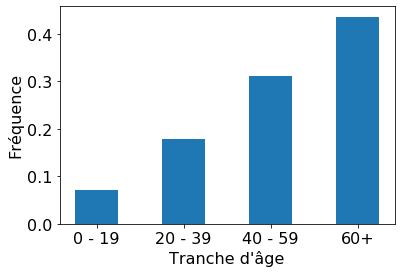
\includegraphics[width=.5\textwidth]{figures/stats/remboursement_age_bars}
%   \caption{Diagramme en b�tons de la fr�quence des tranches d'�ges dans les
%     donn�es du tableau~\ref{tab:remboursement_data}.}
%   \label{fig:remboursement_age_bars}
% \end{figure}
\begin{figure}[h]
  \centering
    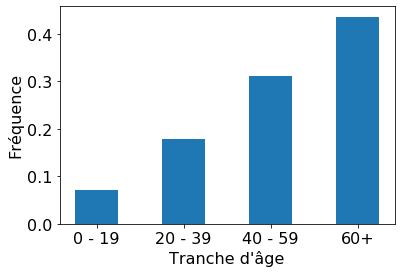
\includegraphics[width=.5\textwidth]{figures/stats/remboursement_age_bars}
  \caption{Diagramme en b�tons de la fr�quence des tranches d'�ges dans les
    donn�es de remboursement.}
  \label{fig:remboursement_age_bars}
\end{figure}

Dans le cas d'une variable continue, la constitution des classes de valeurs
d'une s�rie statistique est une �tape importante. La \textbf{r�gle de Sturges}
propose de d�couper les valeurs observ�es en $\lfloor 1 + \log_2(n)\rfloor$
intervalles de m�me taille $\frac{\max(x_i) - \min(x_i)}{k}$. Cependant, cette
r�gle suppose que la variable analys�e suive une distribution gaussienne ; elle
n'est pas appropri�e, par exemple, si les valeurs s'�talent sur plusieurs
�chelles de grandeur, auquel cas une transformation logarithmique s'imposera.

% Cela nous permet ensuite de construire une \textbf{table des fr�quences} qui
% associe � chaque classe de valeurs la fr�quence de cette valeur dans la
% population observ�e.

\begin{exemple}
  Prenons par exemple, 31 observations de la temp�rature minimale (en
  \si{\celsius}) pour la station m�t�o de Paris-Montsouris, telles que relev�es
  dans la premi�re colonne de la table~\ref{tab:meteo_data}.

  Nous disposons de $n=31$ observations, qu'il s'agit, en appliquant la r�gle de
  Sturges, de grouper en 5 intervalles d'amplitude 2,24\si{\celsius}. La table
  des fr�quences des temp�ratures minimales est donn�e dans le
  tableau ci-dessous : \par % ~\ref{tab:meteo_tmin_freq}.
  % \begin{table}[h]
    \centering
    \begin{tabular}[h]{|l|c|c|c|c|c|} \hline 
      T min (\si{\celsius}) & < -0,16 & -0,16 -- 2,08 & 2,08 -- 4,32 & 4,32 -- 6,56 & > 6,56 \\ \hline 
      Fr�quence & 0,19 & 0,19 & 0,29 & 0,10 & 0,23 \\ \hline
    \end{tabular}
  %   \caption{Table des fr�quences des temp�ratures minimales du tableau~\ref{tab:meteo_data}.}
  %   \label{tab:meteo_tmin_freq}
  % \end{table}
\end{exemple}

Pour une variable continue, la table des fr�quences peut �tre traduite en
\textbf{histogramme,} comme illustr� sur la figure~\ref{fig:meteo_tmin_hist}.

Utiliser des fr�quences plut�t que des comptes permet de comparer des
populations de taille diff�rente. De plus, la distribution des fr�quences
d'une s�rie statistique de la variable $x$, repr�sent�e visuellement par un
histogramme, peut �tre consid�r�e comme une approximation de la distribution de
la probabilit� de cette variable dans la population.

\begin{figure}[h]
  \centering
  \includegraphics[width=.5\textwidth]{figures/stats/meteo_tmin_hist}
  \caption{Histogramme des temp�ratures minimales dans le
    tableau~\ref{tab:meteo_data}.}
  \label{fig:meteo_tmin_hist}
\end{figure}


\paragraph{Fr�quences cumul�es} 
On peut aussi choisir de repr�senter plut�t les \textbf{fr�quences cumul�es.} 

\begin{exemple}
  Pour notre s�rie de temp�ratures minimales, la table des fr�quences cumul�es
  est donn�e dans le tableau ci-dessous : \par % ~\ref{tab:meteo_tmin_cumul_freq}.
  % \begin{table}[h]
    \centering
    \begin{tabular}[h]{|l|c|c|c|c|c|} \hline 
      T min (\si{\celsius}) & < -0,16 & < 2,08 & < 4,32 & < 6,56 & < 8,80 \\ \hline 
      Fr�quence & 0,19 & 0,38 & 0,67 & 0,77 & 1,0 \\ \hline
      T min (\si{\celsius}) & > -2,40 & > -0,16 & > 2,08 & > 4,32 & > 6,56 \\ \hline 
      Fr�quence & 1,0 & 0,81 & 0,62 & 0,33 & 0,23 \\ \hline
    \end{tabular}
  %   \caption{Table des fr�quences cumul�es pour les temp�ratures minimales 
  %     du tableau~\ref{tab:meteo_data}.}
  %   \label{tab:meteo_tmin_cumul_freq}
  % \end{table}
\end{exemple}

Une table des fr�quences cumul�es croissantes et d�croissantes peut
directement �tre traduite en \textbf{courbes des fr�quences cumul�es,} comme
illustr� sur la figure~\ref{fig:meteo_tmin_cumul_freq}.
\begin{figure}[h]
  \centering
  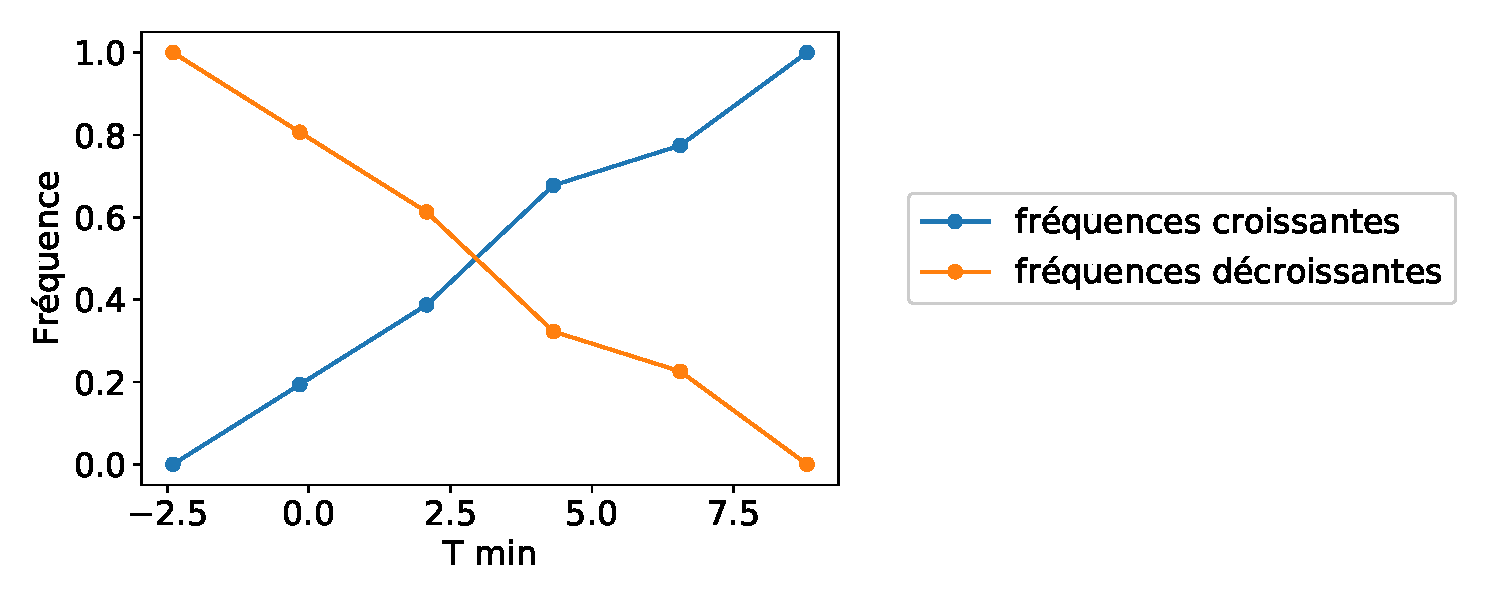
\includegraphics[width=.8\textwidth]{figures/stats/meteo_tmin_cumul_freq}
  \caption{Courbes des fr�quences cumul�es pour les temp�ratures minimales du
    tableau~\ref{tab:meteo_data}.}
  \label{fig:meteo_tmin_cumul_freq}
\end{figure}

\subsection{Indicateurs num�riques}
Enfin, des \textbf{indicateurs num�riques} permettent de compl�ter cette
description. On distinguera les \textbf{indicateurs de tendance centrale} qui
indiquent l'ordre de grandeur des valeurs de la s�rie statistique et o� ces
valeurs se rassemblent, des \textbf{indicateurs de dispersion} qui indiquent
l'�talement de ces valeurs.

\paragraph{Indicateurs de tendance centrale} Les indicateurs de tendance centrale comportent :
\begin{itemize}
\item la \textbf{moyenne arithm�tique} 
\[\bar x = \frac1n \sum_{i=1}^n x_i,\]
La  moyenne arithm�tique peut �tre tr�s sensible � la pr�sence de valeurs aberrantes.
\item la \textbf{m�diane,} qui correspond � une fr�quence cumul�e de 50\%, 
\item le \textbf{mode,} qui est la valeur la plus fr�quente dans la s�rie
  statistique. Le mode n'a r�ellement de sens que pour une variable discr�te ;
  dans le cas d'une variable continue, on parlera plut�t, lorsque la s�rie est
  class�e, de \textbf{classe modale} qui est la classe la plus fr�quente.
\end{itemize}

\begin{exemple}
  Pour notre s�rie de temp�ratures minimales,
  \begin{itemize}
  \item la moyenne arithm�tique vaut $3,2 \si{\celsius}$ ;
  \item la m�diane vaut $4 \si{\celsius}$ ;
  \item la classe modale est $2,1$ -- $4,4 \si{\celsius}$.
  \end{itemize}
\end{exemple}

\paragraph{Indicateurs de dispersion} Les indicateurs de dispersion comportent : 
\begin{itemize}
\item la \textbf{variance de la s�rie statistique} 
\[ s^2(x_1, x_2, \dots, x_n) = \frac1n \sum_{i=1}^n (x_i - \bar x)^2,\]
\item la \textbf{variance d'�chantillonage} 
  \[ s^{*2}(x_1, x_2, \dots, x_n) = \frac1{n-1} \sum_{i=1}^n (x_i - \bar
    x)^2,\]
  La variance d'�chantillonage est d'autant plus proche de la variance que le
  nombre d'observations est grand. Nous verrons dans la
  section~\ref{sec:biais_estimateur} qu'il s'agit d'un estimateur
  \textbf{non-biais�} de la variance de la population.
\item l'\textbf{�cart-type} qui est la racine carr�e de la variance, 
\item le \textbf{coefficient de variation} 
  \[ \text{CV}(x_1, x_2, \dots, x_n) = \frac{s^2(x_1, x_2, \dots, x_n)}{\bar
      x}\]
  Le coefficient de variation permet d'appr�cier la variabilit� d'une variable
  en fonction de sa valeur moyenne, et n'a de sens que pour une variable donn�e
  sur une �chelle dot�e d'un z�ro absolu, c'est-�-dire dans laquelle une valeur
  de $2z$ peut effectivement �tre consid�r�e comme deux fois plus qu'une valeur
  de $z$ (ce n'est pas le cas pour une temp�rature en degr�s Celsius :
  10\si{\celsius} n'est pas � deux fois plus chaud � que 5 \si{\celsius}). De
  plus, il est num�riquement instable quand $\bar x$ est proche de 0.
\end{itemize}

\begin{exemple}
  La variance de notre s�rie de temp�ratures minimales vaut $10,02 \si{\celsius^2}$,
  tandis que la variance d'�chantillonage vaut $10,36 \si{\celsius^2}$. Les
  �carts-types correspondants valent tous les deux $3,2 \si{\celsius}$.  Le
  coefficient de variation n'a pas de sens en degr�s Celsius.
\end{exemple}
\paragraph{Remarques}
\begin{itemize}
\item L'�cart-type d'une variable, qui s'exprime dans la m�me unit� que la
  variable, est beaucoup plus facile � interpr�ter que la variance. On donne
  plus facilement un sens � $3,2 \si{\celsius}$ qu'� $10,02 \si{\celsius^2}$.
\item L'�cart-type est utilis� pour d�finir une erreur de mesure. Imaginons que
  l'on prenne 10 fois la m�me mesure, obtenant ainsi une population de 10
  mesures, de moyenne arithm�tique $m$ et d'�cart-type $\sigma$ ; on rapporte
  alors une valeur de $m \pm \sigma$. Cette remarque est une br�ve incursion
  dans le domaine de la \textit{m�trologie}.
\end{itemize}

Enfin, les \textbf{quantiles} permettent aussi de d�terminer la dispersion
d'une variable. Les $q$-quantiles divisent les valeurs prises par la variable
en $q$ intervalles de m�mes fr�quences. Le $p$-�me $q$-quantile de
$(x_1, x_2, \dots, x_n)$ est d�fini comme la valeur $Q_p^q$ telle que 
\[\text{Freq}(x \leq Q_p) = \frac{p}{q}.\]

Lorsque $q=4,$ on parle de \textbf{quartiles.} Lorsque $q=10,$ on parle de
\textbf{d�ciles.}

\begin{exemple}
  Les trois quartiles de notre s�rie de temp�ratures minimales sont
  $0,8 \si{\celsius}$, $4,0 \si{\celsius}$ et $5,6 \si{\celsius}$ : 25\% des
  valeurs observ�es sont inf�rieures � $0,8 \si{\celsius}$, 50\% sont inf�rieures
  � 4,0 \si{\celsius} et 75\% sont inf�rieures � $5,6 \si{\celsius}$. Le deuxi�me
  quartile correspond bien � la m�diane.
\end{exemple}

Une \textbf{bo�te � moustaches} (ou \textit{boxplot}) permet de r�sumer
visuellement ces indicateurs, comme illustr� sur la
figure~\ref{fig:meteo_tmin_boxplot}. La bo�te � moustaches est compos�e d'un
rectangle, d'une largeur arbitraire et d�limit� en bas par la valeur du premier
quartile et en haut par la valeur du troisi�me quartile ; d'une barre
horizontale au niveau de la m�diane ; et de deux segments joignant chacun les
extr�mit�s du rectangle aux valeurs les plus extr�mes. Repr�senter les valeurs
prises par la variable par un nuage de points superpos� � ce rectangle permet
d'en faciliter l'interpr�tation.

\begin{figure}[h]
  \centering
  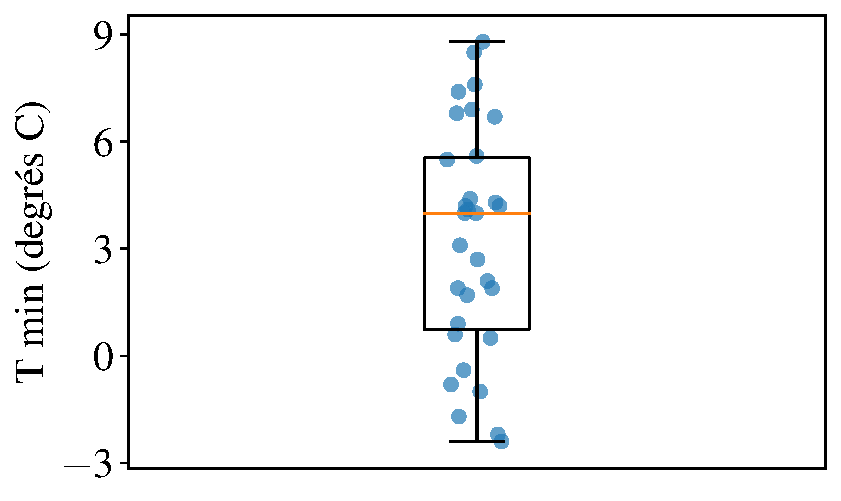
\includegraphics[width=.5\textwidth]{figures/stats/meteo_tmin_boxplot}
  \caption{Bo�te � moustaches des temp�ratures minimales du
    tableau~\ref{tab:meteo_data}.}
  \label{fig:meteo_tmin_boxplot}
\end{figure}

\section{Statistique descriptive bidimensionelle}
Il s'agit ici de mettre en �vidence une �ventuelle \textbf{liaison,}
c'est-�-dire une variabilit� simultan�e, entre deux variables statistiques $x$
et $y$, observ�es sur $n$ individus, � travers les s�ries statistiques
$(x_1, x_2, \dots, x_n)$ et $(y_1, y_2, \dots, y_n).$

Cette liaison peut �tre causale ou non. Mettre en �vidence une causalit� est
d�licat, et d�passe le cadre de ce cours.

Comprendre la liaison entre deux variables nous permet de comprendre 
\begin{itemize}
\item Si une variable peut d�pendre d'une autre : la temp�rature minimale
  d�pend-elle de l'ensoleillement ?
\item Si une variable peut permettre de pr�dire une autre : la temp�rature
  minimale permet-elle de pr�dire la temp�rature maximale ?
\item Si une variable peut �tre remplac�e par une autre : ai-je besoin de
  prendre en compte et la temp�rature minimale et la temp�rature maximale, ou
  la temp�rature moyenne suffit-elle ?
\end{itemize}

\subsection{Liaison entre deux variables quantitatives}

\paragraph{Nuage de points}
Pour visualiser la liaison entre deux variables quantitatives, on utilise
g�n�ralement un \textbf{nuage de points}. Si $x$ et $y$ sont homog�nes,
c'est-�-dire exprim�es dans la m�me unit�, on utilisera la m�me �chelle sur les
deux axes, comme sur la figure~\ref{fig:meteo_tmin_tmax}. Sinon, on pr�f�rera
g�n�ralement centrer et r�duire les variables au pr�alable, comme sur la
figure~\ref{fig:meteo_tmin_vent} : 
\[
  x_i \leftarrow \frac{x_i - \bar x}{\sigma_x} \qquad \text{avec } \bar x = \sum_{i=1}^n x_i 
  \text{ et } \sigma_x = \sqrt{\sum_{i-1}^n(x_i - \bar x)^2}.
\]

\begin{figure}[h]
  \centering
  \begin{subfigure}[t]{0.49\textwidth}
    \centering
    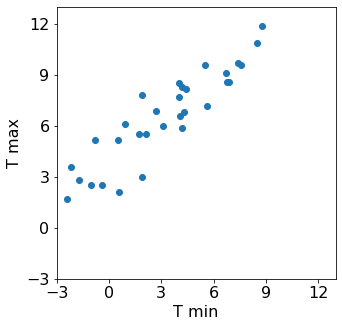
\includegraphics[width=.7\textwidth]{figures/stats/meteo_tmin_tmax}
    \caption{Temp�ratures maximales vs minimales.}
    \label{fig:meteo_tmin_tmax}
  \end{subfigure} \hfill
  \begin{subfigure}[t]{0.49\textwidth}
    \centering
    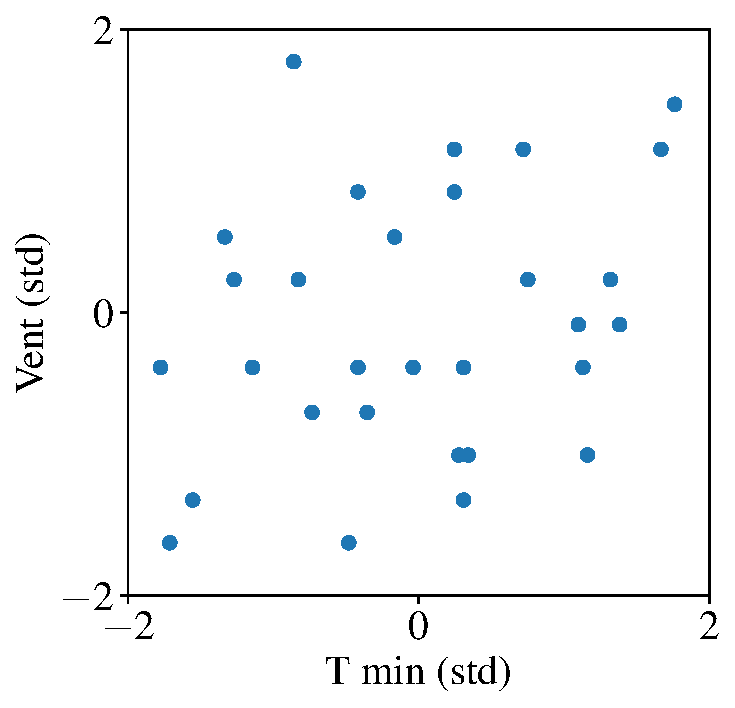
\includegraphics[width=.7\textwidth]{figures/stats/meteo_tmin_vent}
    \caption{Vent vs temp�ratures minimales.}
    \label{fig:meteo_tmin_vent}
  \end{subfigure}
  \caption{Nuages de points pour des paires de variables du
    tableau~\ref{tab:meteo_data}.}
\end{figure}


\paragraph{Indicateurs de liaison entre deux variables quantitatives}
Pour quantifier la liaison entre deux variables quantitatives, on utilise
principalement
\begin{itemize}
\item \textbf{la covariance}
\[s(x, y) = \frac1n \sum_{i=1}^n (x_i - \bar x) (y_i - \bar y).\]
\item \textbf{le coefficient de corr�lation de Pearson,} qui est �gal � la
  covariance entre les variables centr�es r�duites, et compris entre $-1$ et $1$ :
\[r(x, y) = \frac1n \frac{\sum_{i=1}^n (x_i - \bar x) (y_i - \bar y)}{\sigma_x, \sigma_y.}\]
\end{itemize}

� noter que la covariance et le coefficient de corr�lation de Pearson mesurent
des liaisons \textit{lin�aires} entre deux variables. Une corr�lation de
Pearson proche de 1 ou de -1 indique une relation lin�aire ; une corr�lation de
Pearson proche de 0 indique une absence de corr�lation. D'autres mesures, comme
l'information mutuelle (hors cadre de ce cours), permettent de mesurer des
liaisons \textit{non-lin�aires}. 

\begin{exemple}
  Pour les donn�es du tableau~\ref{tab:meteo_data}, la covariance entre la
  temp�rature minimale et la temp�rature maximale vaut $7,69 \si{\celsius^2}$ ;
  leur corr�lation de Pearson vaut 0,91. La corr�lation de Pearson entre vent
  et temp�rature minimale vaut 0,28. La figure~\ref{fig:pearson} illustre le
  rapport entre corr�lation de Pearson et nuage de points.
\end{exemple}
\begin{figure}[h]
  \centering
    \begin{subfigure}[t]{0.24\textwidth}
      \centering
      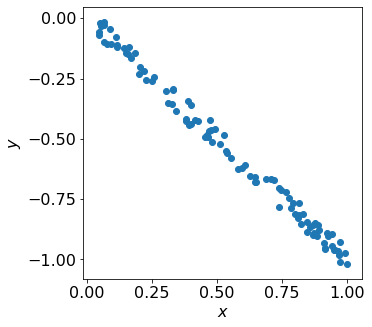
\includegraphics[width=\textwidth]{figures/stats/pearson_3}
      \caption{r(x, y) = -1,00.}
    \end{subfigure} \hfill
    \begin{subfigure}[t]{0.24\textwidth}
      \centering
      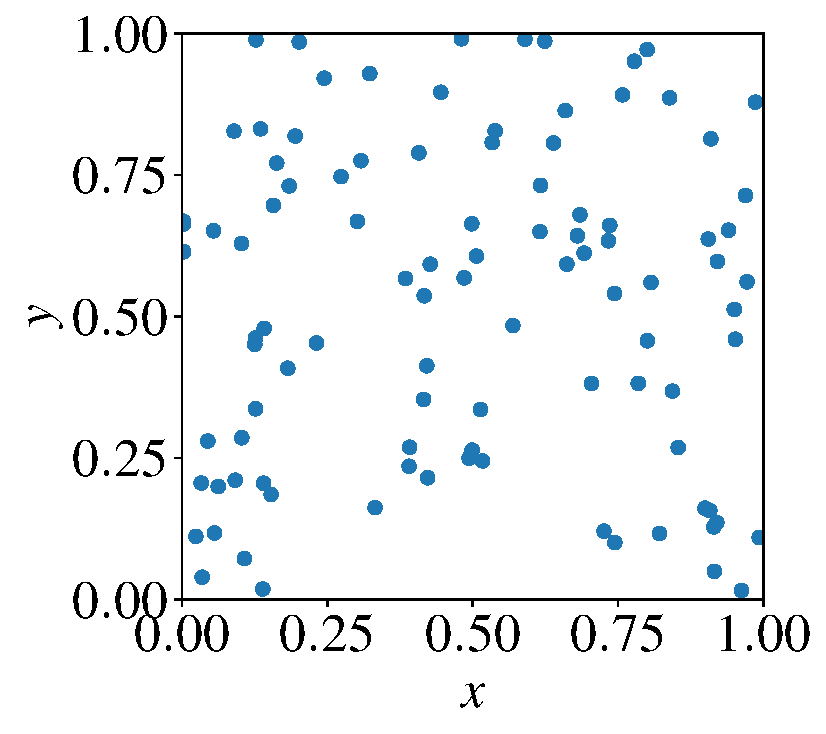
\includegraphics[width=\textwidth]{figures/stats/pearson_0}
      \caption{r(x, y) = 0,03.}
    \end{subfigure} \hfill
    \begin{subfigure}[t]{0.24\textwidth}
      \centering
      \includegraphics[width=\textwidth]{figures/stats/pearson_2}
      \caption{r(x, y) = 0,53.}
    \end{subfigure} \hfill
    \begin{subfigure}[t]{0.24\textwidth}
      \centering
      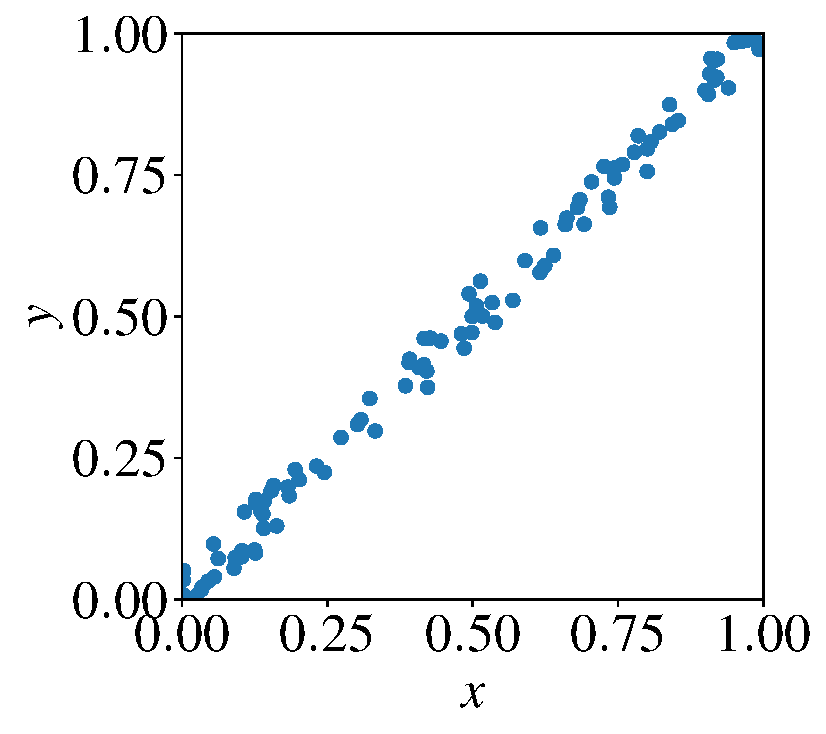
\includegraphics[width=\textwidth]{figures/stats/pearson_1}
      \caption{r(x, y) = 1,00.}
    \end{subfigure} \hfill
  \caption{Nuages de points entre deux variables simul�es et leur corr�lation de Pearson.}
  \label{fig:pearson}
\end{figure}

\paragraph{Indicateurs de liaison entre une variable qualitative et une variable quantitative}
Pour �tudier la liaison entre une variable qualitative $x$, ayant $K$ modes (ou
valeurs diff�rentes) dans la s�rie statistique $(x_1, x_2, \dots, x_n),$ et une
variable quantitative $y,$ on consid�re que la variable $x$ permet de d�finir
$p$ sous-populations. Il s'agit alors d'�valuer s'il existe des diff�rences,
pour la variable $y$, entre ces sous-populations.

Visuellement, on utilisera une s�rie de bo�tes � moustaches, comme illustr� sur
la figure~\ref{fig:remboursement_rembourses_age}.

% \begin{figure}[h]
%   \centering
%   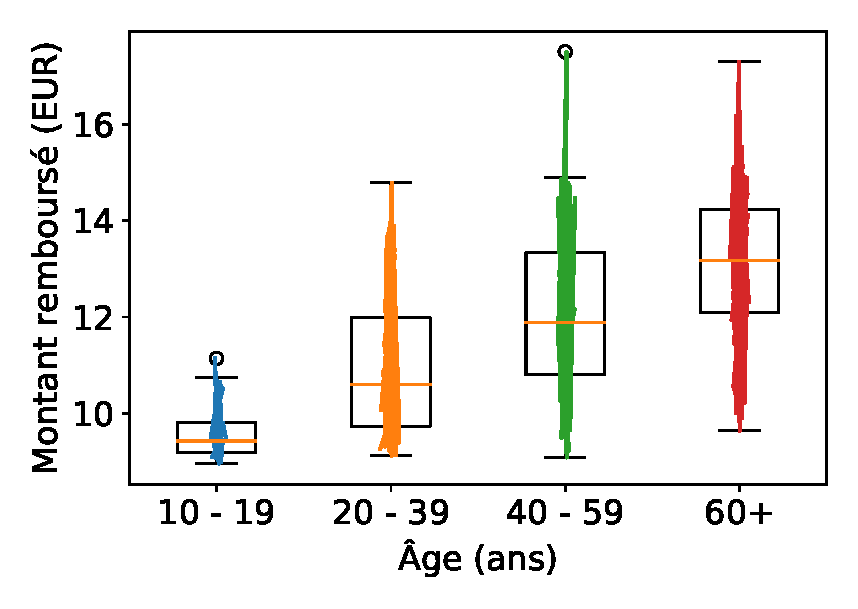
\includegraphics[width=.5\textwidth]{figures/stats/remboursement_rembourses_age}
%   \caption{Montants rembours�s par acte, par tranche d'�ge, pour les donn�es du
%     tableau~\ref{tab:remboursement_data}.}
%   \label{fig:remboursement_rembourses_age}
% \end{figure}
\begin{figure}[h]
  \centering
  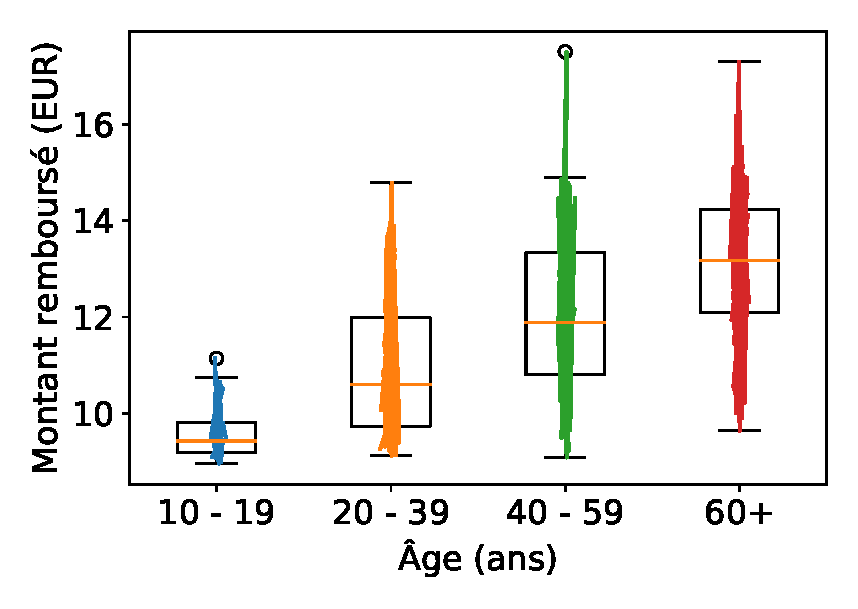
\includegraphics[width=.5\textwidth]{figures/stats/remboursement_rembourses_age}
  \caption{Montants rembours�s par acte, par tranche d'�ge, pour les donn�es de
    remboursement.}
  \label{fig:remboursement_rembourses_age}
\end{figure}

La \textbf{variance expliqu�e} par $x$ de $y$ la moyenne des carr�s des �carts
entre la moyenne de $y$ dans chaque sous-population et la moyenne de $y$ dans
toute la population, pond�r�e par la taille des sous-populations :
\[
  \sigma_E^2 = \frac1n \sum_{k=1}^K n_k (\bar{y}_k - \bar{y})^2,
\]
o� $\bar{y}_k$ est la moyenne de $y$ dans la sous-population $k$ et $\bar{y}$
la moyenne de $y$ dans la population totale.

La \textbf{variance r�siduelle} est la moyenne des variances des
sous-populations, pond�r�es par leur taille :
\[
  \sigma_R^2 = \frac1n \sum_{k=1}^K n_k \sigma_k^2, 
\]
o� $n_k$ est le nombre d'individus dans la sous-population $k$ et $\sigma_k^2$
est la variance de $y$ dans cette sous-population.


On peut montrer que $\sigma_y^2 = \sigma_R^2 + \sigma_E^2.$

Le \textbf{rapport de corr�lation} est la part de variation de $y$ expliqu�e
par $x$. Compris entre 0 et 1, il est d'autant plus �lev� que la liaison entre
les deux variables est forte :
\[
e^2  = \frac{\sigma_E^2}{\sigma_y^2}.
\]
\begin{exemple}
% Pour les montants rembours�s par acte du tableau~\ref{tab:remboursement_data},
% la variance de ces montants est de 3,65, tandis que la variance expliqu�e par
% l'�ge est de 1,37 (en euros au carr�), ce qui donne un rapport de corr�lation
% de 0,38.
  Pour les montants rembours�s par acte de nos donn�es de remboursement, la
  variance de ces montants est de $3,30\texteuro^2$, tandis que la variance
  expliqu�e par l'�ge est de $1,09\texteuro^2$, ce qui donne un rapport de
  corr�lation de $0,33.$ 
\end{exemple}

\paragraph{Indicateurs de liaison entre deux variables qualitatives}
Pour �tudier la liaison entre une variable qualitative $x$, ayant $K$ modes (ou
valeurs diff�rentes) dans la s�rie statistique $(x_1, x_2, \dots, x_n),$ et une
variable qualitative $y$, ayant $L$ modes dans la s�rie statistique
$(y_1, y_2, \dots, y_n),$ on utilise g�n�ralement une \textbf{table de
  contingence} $A$ de taille $K \times L.$ Il s'agit de compter, pour chaque
mode de $x$ et chaque mode de $y$, combien d'individus pr�sentent ces deux
modes : $A_{ij}$ est le nombre d'invididus pour lesquels $x = i$ et $y = j$.

Si l'on appelle $N = \sum_{k=1}^K \sum_{l=1}^L A_{kl}$ le nombre total
d'individus, $N_{i.} = \sum_{l=1}^L A_{il}$ le nombre d'individus dans la ligne
$i$ et $N_{.j} = \sum_{k=1}^K A_{kj}$ le nombre d'individus dans la colonne $j$,
alors l'absence de liaison entre $x$ et $y$ se traduit par 
\[
  \frac{N_{ij}}{N} = \frac{N_{i.}}{N}
  \frac{N_{.j}}{N} \text{ pour tout } 
  1 \leq i \leq K, 1 \leq j \leq L.
\]
L'�cart entre les valeurs prises de part et d'autre de cette �galit� se mesure
gr�ce � la \textbf{distance du chi2}, d�finie par 
\[
d_{\chi^2} = \sum_{i=1}^K \sum_{j=1}^L  \frac{\left( A_{ij} - 
    \frac{N_{i.}N_{.j}}{N} \right)^2}{\frac{N_{i.}N_{.j}}{N}}
\]

\begin{exemple}
  La table de contingence pour les variables � �ge � et � r�gion � des donn�es
  de remboursement est donn�e dans le
  tableau~\ref{tab:remboursement_age_region}. La distance du chi2 pour cette
  table de contingence est de 11,21, ce qui sugg�re une d�pendance entre les
  variables � �ge � et � r�gion � dans les donn�es.
  \begin{table}[h]
    \centering
    \begin{tabular}[h]{|c|c|c|c|c|c|c|c|c|c|c|c|c|c|}
      \hline
      & \multicolumn{13}{|c|}{R�gion} \\ \hline
      {�ge} & 5 & 11 & 24 & 27 & 28 & 32 & 44 & 52 & 53 & 75 & 76 & 84 & 93 \\ \hline
      0--19 & 3 & 5 & 3 & 3 & 3 & 3 & 4 & 3 & 2 & 3 & 3 & 4 & 4 \\ \hline
      20--39 & 8 & 18 & 4 & 7 & 4 & 9 & 11 & 6 & 4 & 7 & 8 & 10 & 11 \\ \hline
      40--59 & 11 & 26 & 11 & 13 & 13 & 16 & 15 & 10 & 8 & 12 & 17 & 15 & 19 \\ \hline
      $>$ 60 & 15 & 31 & 18 & 16 & 21 & 21 & 22 & 12 & 12 & 19 & 24 & 23 & 26 \\ \hline
    \end{tabular}
    \caption{Table de contingence pour l'�ge et la r�gion des donn�es 
      de remboursement.}
    \label{tab:remboursement_age_region}
  \end{table}
\end{exemple}

Nous verrons au chapitre~\ref{chap:tests} comment transformer cette distance en
un test statistique de d�pendance.

% \begin{table}[h]
%   \centering
%   \begin{tabular}[h]{|c|c|c|c|c|c|c|c|c|c|c|}
%     \hline
%     & \multicolumn{10}{|c|}{R�gion} \\ \hline
%     {�ge} & 5 & 11 & 24 & 27 & 32 & 44 & 75 & 76 & 84 & 93 \\ \hline
%     20--39 & 1 & 1 & 0 & 0 & 2 & 0 & 0 & 0 & 0 & 0 \\ \hline
%     40--59 & 0 & 1 & 0 & 0 & 1 & 1 & 0 & 1 & 1 & 0 \\ \hline
%     $>$ 60 & 1 & 1 & 1 & 1 & 2 & 1 & 1 & 2 & 0 & 1 \\ \hline
%   \end{tabular}
%   \caption{Table de contingence pour l'�ge et la r�gion des donn�es 
%     du tableau~\ref{tab:remboursement_data}.}
%   \label{tab:remboursement_age_region}
% \end{table}

La table de contingence peut �tre visualis�e gr�ce � deux \textbf{diagrammes en
  barres empil�es} : on peut choisir de visualiser, pour chaque mode de $x$, la
proportion relative des modes de $y$, ou inversement, pour chaque mode de $y$,
la proportion relative des modes de $x$. Ces deux choix sont illustr�s sur les
figures~\ref{fig:remboursement_age_region_lines}
et~\ref{fig:remboursement_age_region_cols} respectivement.

\begin{figure}[h]
  \centering
  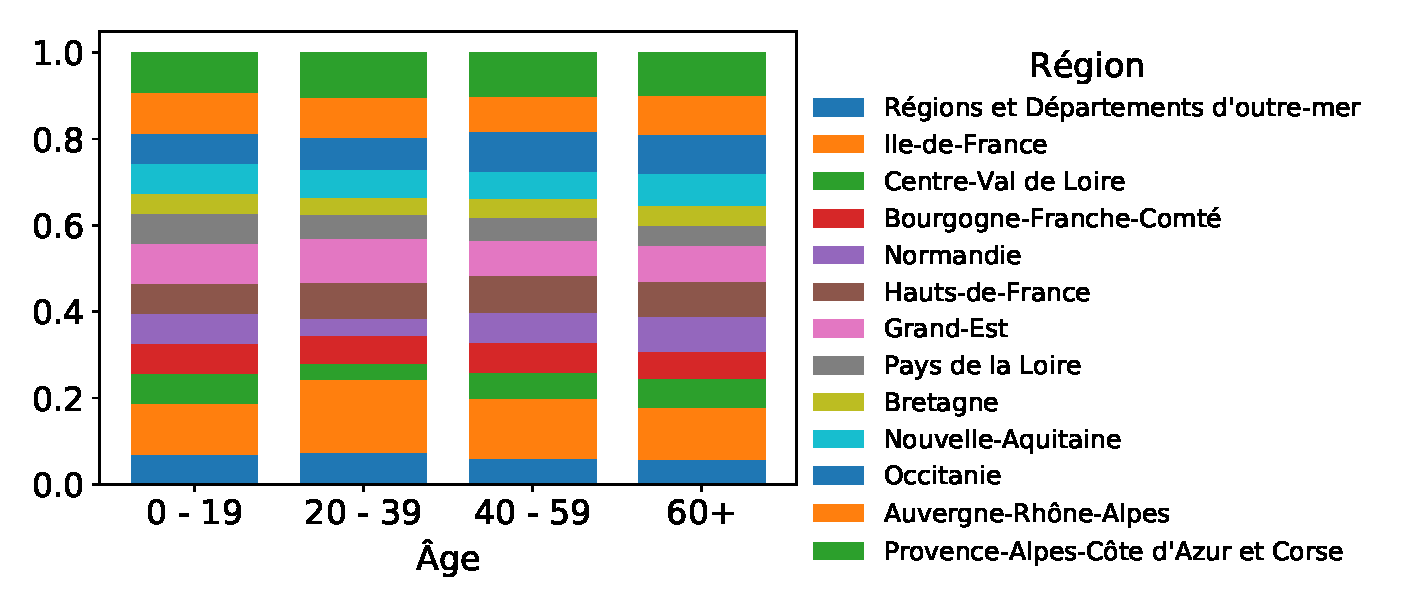
\includegraphics[width=\textwidth]{figures/stats/remboursement_age_region_lines}
  \caption{Diagramme en barres repr�sentant, pour chaque tranche d'�ges, la
    proportion relative d'individus de chaque r�gion dans la table de
    contingence du tableau~\ref{tab:remboursement_age_region}.}
  \label{fig:remboursement_age_region_lines}
\end{figure}

\begin{figure}[h]
  \centering
  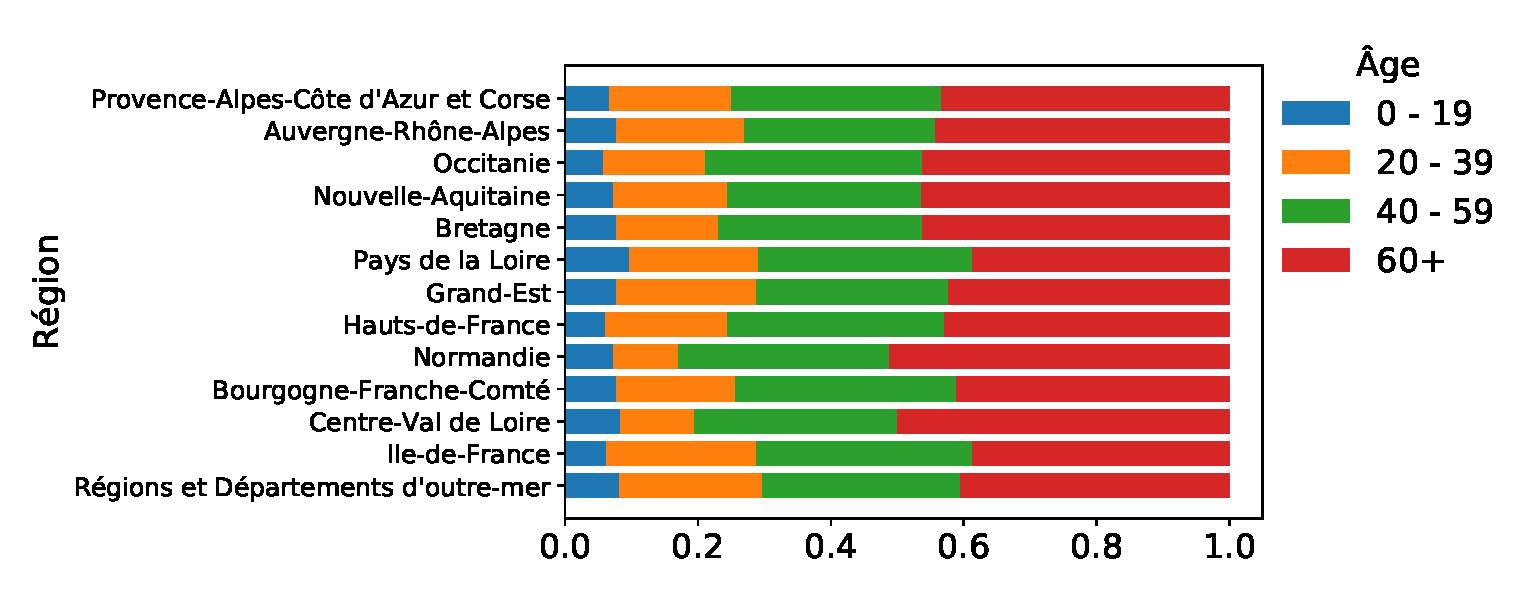
\includegraphics[width=\textwidth]{figures/stats/remboursement_age_region_cols}
  \caption{Diagramme en barres repr�sentant, pour chaque r�gion, la proportion
    relative d'individus de chaque tranche d'�ge dans la table de contingence du
    tableau~\ref{tab:remboursement_age_region}.}
  \label{fig:remboursement_age_region_cols}
\end{figure}

% Pour �tudier la table de contingence, on pourra en calculer les \textbf{profils
%   lignes} et les \textbf{profils colonnes} : il s'agit de normaliser les
% entr�es par le nombre d'individus par ligne ou, respectivement, par colonne.

% \begin{table}[h]
%   \centering
%   \begin{tabular}[h]{|c|c|c|c|c|c|c|c|c|c|c|}
%     \hline
%     & \multicolumn{10}{|c|}{R�gion} \\ \hline
%     {�ge} & 5 & 11 & 24 & 27 & 32 & 44 & 75 & 76 & 84 & 93 \\ \hline
%     20--39 & 0.25 & 0.25 & 0 & 0 & 0.50 & 0 & 0 & 0 & 0 & 0 \\ \hline
%     40--59 & 0 & 0.20 & 0 & 0 & 0.20 & 0.20 & 0 & 0.20 & 0.20 & 0 \\ \hline
%     $>$ 60 & 0.09 & 0.09 & 0.09 & 0.09 & 0.18 & 0.09 & 0.09 & 0.18 & 0 & 0.09 \\ \hline
%   \end{tabular}
%   \caption{Profils lignes (c'est-a-dire par �ge) pour la table de contingence 
%     donn�e dans le tableau~\ref{tab:remboursement_age_region}.}
%   \label{tab:remboursement_age_region_ligne}
% \end{table}

% \begin{table}[h]
%   \centering
%   \begin{tabular}[h]{|c|c|c|c|c|c|c|c|c|c|c|}
%     \hline
%     & \multicolumn{10}{|c|}{R�gion} \\ \hline
%     {�ge} & 5 & 11 & 24 & 27 & 32 & 44 & 75 & 76 & 84 & 93 \\ \hline
%     20--39 & 0.50 & 0.33 & 0 & 0 & 0.40 & 0    & 0 & 0    & 0 & 0 \\ \hline
%     40--59 & 0    & 0.33 & 0 & 0 & 0.20 & 0.50 & 0 & 0.33 & 1 & 0 \\ \hline
%     $>$ 60 & 0.50 & 0.33 & 1 & 1 & 0.40 & 0.50 & 1 & 0.67 & 0 & 1 \\ \hline
%   \end{tabular}
%   \caption{Profils colonnes (c'est-a-dire par r�gion) pour la table de contingence 
%     donn�e dans le tableau~\ref{tab:remboursement_age_region}.}
%   \label{tab:remboursement_age_region_colonne}
% \end{table}


% \begin{itemize}
% \item cf cours Laure Reboul.
% \item Utiliser http://iml.univ-mrs.fr/~reboul/enseignement.html pour proposer des exercices ?
% \end{itemize}


% Les donn�es du tableau~\ref{tab:remboursement_data} ont �t� extraites parmi les
% 604 individus constituant la population totale. La \textbf{table des
%   fr�quences} des �ges dans la population totale est donn�e dans le
% tableau~\ref{tab:remboursement_age_freq_total}.
% \begin{table}[h]
%   \centering
%   \begin{tabular}[h]{|l|c|c|c|c|c|} \hline 
%     Tranche d'�ge (ans) & 20 -- 39 & 40 -- 59 & $>$ 60 \\ \hline     
%     Fr�quence & 19\% & 31\% & 43\% \\ \hline
%   \end{tabular}
%   \caption{Table des fr�quences des �ges parmi les 604 individus 
%     parmi lesquels ceux du tableau~\ref{tab:remboursement_data} 
%     ont �t� �chantillonn�s.}
%   \label{tab:remboursement_age_freq_total}
% \end{table}


% Ces valeurs sont assez �loign�es de celles du tableau~\ref{tab:remboursement_age_freq}.


%%% Local Variables:
%%% mode: latex
%%% TeX-master: "sdd_2020_poly"
%%% End:
\clearpage 

\chapter{Estimation}
%-*- coding: iso-latin-1 -*-
\label{chap:estimation}

\paragraph{Notions :} �chantillon al�atoire, estimateur, estimation, biais d'un
estimateur, convergence d'un estimateur, estimation par maximisation de la
vraisemblance.
\paragraph{Objectifs p�dagogiques :}
\begin{itemize}
\item Choisir un estimateur, en particulier en d�terminant des propri�t�s
  telles que son biais, sa variance, ou sa convergence.
\item Proposer un estimateur, en particulier par maximisation de la
  vraisemblance.
\end{itemize}


\section{Inf�rence statistique}
Alors que la statistique descriptive se contente de \textit{d�crire} une
population ou un �chantillon de celle-ci, l'inf�rence statistique cherche �
tirer des conclusions sur une population � partir de l'�tude d'un �chantillon
de celle-ci. % Pour cela, il est n�cessaire de s'int�resser :
% \begin{itemize}
% \item aux techniques d'\textbf{�chantillonnage} (cf section~\ref{sec:echantilonnage})
%   permettant de construire des �chantillons d'une population ;
% \item � la \textbf{mod�lisation} permettant de supposer un mod�le probabiliste
%   sur la population ;
% \item aux techniques d'\textbf{estimation} (cf section~\ref{sec:estimation})
%   permettant de d�terminer (approximativement) un param�tre d'une population �
%   partir d'un �chantillon de celle-ci ;
% \item aux \textbf{tests d'hypoth�se} (cf chapitre~\ref{chap:tests}) permettant de valider
%   ou d'infirmer des hypoth�ses sur la population.
% \end{itemize}

\section{�chantillonnage}
\label{ref:echantilonnage}

Lorsque la population � �tudier est trop grande pour qu'il soit possible
d'observer chacun de ses individus, on �tudie alors une partie seulement de la
population. Cette partie est appel�e \textbf{�chantillon}. On parle alors de
\textbf{sondage}, par opposition � un \textbf{recensement}, qui consiste �
�tudier tous les individus d'une population.

\paragraph{Hypoth�ses de l'�chantillonnage} Pour tirer parti d'un �chantillon, nous allons avoir besoin des hypoth�ses suivantes :

\begin{itemize}
\item La taille de la population est infinie ;
\item Les variables mesur�es sur la population peuvent �tre consid�r�es comme
  des variables al�atoires, dont les mesures sont des r�alisations. Les lois de
  probabilit� suivies par ces variables peuvent appartenir � une famille connue
  (e.g. loi gaussienne, loi de Poisson, etc.) ou �tre totalement
  inconnues. Dans le premier cas, on parlera de \textbf{statistique
    inf�rentielle param�trique} ; dans le deuxi�me, de \textbf{statistique
    inf�rentielle non-param�trique}.
\end{itemize}

\paragraph{Objectifs de la statistique inf�rentielle} La statistique
inf�rentielle a alors pour but d'\textbf{identifier les lois de probabilit� des
  variables al�atoires} en d�crivant les variables. Cela peut prendre les
formes suivantes :

\begin{itemize}
\item L'estimation, qui permet d'approcher les param�tres des lois (param�tre
  $p$ d'une loi de Bernoulli, indice et param�tre d'�chelle d'une loi Gamma) ou
  certaines de leurs caract�ristiques (esp�rance, variance, moments d'ordre
  sup�rieur, quartiles, etc.). C'est le sujet de ce chapitres.
\item Les tests d'hypoth�se, qui permettent d'infirmer ou de confirmer des
  hypoth�ses faites sur ces lois, leurs param�tres ou leurs
  caract�ristiques. Il s'agit par exemple de d�cider s'il est plausible que
  l'esp�rance d'une variable soit sup�rieure � une certaine valeur ; ou qu'une
  variable suive une loi normale. C'est le sujet du prochain chapitre.
\end{itemize}

\subsection{�chantillonnage al�atoire}
Dans la suite de ce chapitre, nous allons consid�rer que l'�chantillon obtenu
par sondage est obtenu par \textbf{�chantillonnage al�atoire simple} : on
pr�l�ve des individus dans la population au hasard, sans remise. Chaque
individu de la population a la m�me probabilit� $1/N$ d'�tre pr�lev�, o� $N$
est la taille de la population (on rappelle que $N \rightarrow \infty$) et ils
sont pr�lev�s ind�pendamment les uns des autres.

\paragraph{Remarque} D'autres techniques d'�chantillonnage sont possibles,
comme l'�chantillonnage al�atoire \textit{stratifi�}, dans lequel la population
est partitionn�e en strates selon une caract�ristique (par exemple, par tranche
d'�ge), et l'�chantillon est obtenu en proc�dant � un �chantillonnage al�atoire
simple dans chacune des strates, permettant d'obtenir pour chaque strate un
�chantillon de taille proportionnelle � la taille de strate dans la
population. Ainsi, les individus n'ont pas tous la m�me probabilit� d'�tre
tir�s : celle-ci d�pend de la taille de la strate � laquelle ils appartiennent.

% \begin{encadre}
  {Deux �chantillons $(x_1, x_2, \dots, x_n)$ et
  $(x^\prime_1, x^\prime_2, \dots, x^\prime_n)$ de tailles identiques $n$ de la
  m�me population seront donc diff�rents. On mod�lise cette variabilit� en
  consid�rant que chacun des individus $x_i$ ou $x^\prime_i$ est la r�alisation
  d'une m�me variable al�atoire $X_i$, o� $(X_1, X_2, \dots, X_n)$ est un
  vecteur al�atoire, dont les composantes sont ind�pendantes et identiquement
  distribu�es. 
  \begin{itemize}
  \item $(X_1, X_2, \dots, X_n)$ est appel� \textbf{�chantillon al�atoire} ;
  \item $(x_1, x_2, \dots, x_n)$ et
    $(x^\prime_1, x^\prime_2, \dots, x^\prime_n)$ sont deux �chantillons,
    c'est-�-dire deux \textit{r�alisations} de cet �chantillon al�atoire.
  \end{itemize}}
%\end{encadre}

Un indicateur statistique de l'�chantillon est alors la r�alisation d'une
variable al�atoire fonction de l'�chantillon al�atoire.

\begin{exemple} La moyenne d'un �chantillon,
$\bar{x} = \frac1n \sum_{i=1}^n x_i,$ est la r�alisation d'une variable
al�atoire $M_n$ d�finie par
\[
  M_n = \frac1n \sum_{i=1}^n X_i,
\]
qui est une fonction de l'�chantillon al�atoire $(X_1, X_2, \dots, X_n)$.
\end{exemple}

\section{Estimation ponctuelle}
Soit $(\Omega, \Acal, \PP)$ un espace probabilis�, $E$ un espace mesurable, et
$X$ une variable al�atoire � valeurs dans $E$. En pratique, dans la suite de ce
chapitre, nous consid�rerons des variables al�atoires r�elles ($E = \RR$ ou une
partie de $\RR$ telle que $\RR_+$ ou $\NN$), mais les id�es qui y sont
pr�sent�es peuvent �tre �tendues � $\RR^d$ ou � des espaces plus sophistiqu�s.

Soit $(X_1, X_2, \dots, X_n)$ un �chantillon al�atoire. Les $X_i$ sont
ind�pendants et identiquement distribu�es, de m�me loi $\PP_X$ que $X.$ Soit
$(x_1, x_2, \dots, x_n)$ un �chantillon, autrement dit une r�alisation de cet
�chantillon al�atoire.

Soit $\theta \in \RR$ une quantit� d�terministe (i.e. il ne s'agit pas d'une
variable al�atoire), qui d�pend uniquement de $\PP_X.$ Le but de l'estimation
ponctuelle est d'approcher au mieux la valeur de $\theta$. 

\begin{exemple} Si l'on fait l'hypoth�se que $X$ suit une loi
exponentielle (statistique inf�rentielle param�trique), on peut chercher �
estimer le param�tre $\theta$ de cette loi. On peut aussi chercher � estimer
l'esp�rance de $\PP_X,$ un de ses moments, un quantile, etc.
\end{exemple}

\subsection{D�finition d'un estimateur}
On appelle \textbf{estimateur} de $\theta$ une statistique de l'�chantillon
al�atoire $(X_1, X_2, \dots, X_n),$ c'est � dire une variable al�atoire
fonction de $(X_1, X_2, \dots, X_n) :$ un estimateur $\Theta_n$ de $\theta$
peut �tre d�fini par 
\[
  \Theta_n = g(X_1, X_2, \dots, X_n), \qquad g: E \rightarrow \RR.
\]

�tant donn� un �chantillon $(x_1, x_2, \dots, x_n)$ de $X$, on appelle
\textbf{estimation} de $\theta$ la valeur
\[
  \hat{\theta}_n = g(x_1, x_2, \dots, x_n) \in \RR,
\]
qui est donc une r�alisation de $\Theta_n$.

\paragraph{R�sum�}
�tant donn� une variable al�atoire r�elle $X$ � valeurs dans $E,$ un entier
$n \in \NN^*$, et une valeur $\theta$ � estimer qui ne d�pend que de la loi de
$X,$
\begin{itemize}
\item un �chantillon al�atoire $(X_1, X_2, \dots, X_n)$ est un vecteur
  al�atoire, dont les composantes sont iid de m�me loi que $X$ ;
\item un �chantillon $(x_1, x_2, \dots, x_n) \in \RR^n$ est une r�alisation de
  ce vecteur al�atoire ;
\item un estimateur de $\theta$ est une variable al�atoire $\Theta_n$ fonction
  de $(X_1, X_2, \dots, X_n)$ : \\ $\Theta_n = g(X_1, X_2, \dots, X_n)$, avec $g: E \rightarrow \RR$ ;
\item une estimation de $\theta$ est une r�alisation $\hat{\theta}_n$ de
  $\Theta_n$ : $\hat{\theta}_n = g(x_1, x_2, \dots, x_n) \in \RR.$
\end{itemize}

\subsection{Exemple : estimation de la moyenne par la moyenne empirique}
Consid�rons maintenant que $X$ est de carr� int�grable ($X \in \Lcal^2$),
d'esp�rance $m$ et de variance $\sigma^2 > 0$.

La \textbf{moyenne empirique} de $X$ est une variable al�atoire $M_n$, d�finie
par
\[
  M_n = \frac1n \sum_{i=1}^n X_i.
\]

$M_n$ est un estimateur de $m$ : �tant donn� un �chantillon
$(x_1, x_2, \dots, x_n),$ la valeur $\hat{m}_n = \frac1n \sum_{i=1}^n x_i$ est
une estimation de $m$.

� ce stade, rien ne nous permet de dire que $M_n$ est un \textit{bon}
estimateur de $m$ ; en effet, nous pourrions aussi d�finir
$\frac2n \sum_{i=1}^n X_i$ comme estimateur de la moyenne. Quelles sont les
\textit{propri�t�s} de $M_n$ qui nous font pr�f�rer poser $M_n$ comme nous
l'avons fait ? Quelques indices :

\begin{itemize}
\item $\EE(M_n) = m.$ Nous verrons que l'on dit que $M_n$ est un estimateur
  \textit{non-biais�} de $m$ (cf. section~\ref{sec:biais_estimateur}) ;
\item $\VV(M_n) = \frac{\sigma^2}{n}$ (voir calcul
  section~\ref{sec:estimation_proofs}) : plus l'�chantillon est grand, plus la
  variance de l'estimateur est faible, autrement dit plus sa r�alisation
  $\hat{m}_n$ sera proche de son esp�rance $m$. On parle ici de la
  \textit{pr�cision} de $M_n$ (cf. section~\ref{sec:precision_estimateur}) ;
\item Par la loi faible des grands nombres, $M_n \cvproba m.$ Nous
  verrons que l'on dit que $M_n$ est un estimateur \textit{convergent} de $m$
  (cf. section~\ref{sec:convergence_estimateur}) ;
\item Par la loi forte des grands nombres, $M_n \cvps m.$ Nous
  verrons que l'on dit que $M_n$ est un estimateur \textit{fortement convergent} de $m$
  (cf. section~\ref{sec:convergence_estimateur}).
\end{itemize}



\section{Propri�t�s d'un estimateur}

\subsection{Biais d'un estimateur}
\label{sec:biais_estimateur}
Le \textbf{biais} d'un estimateur $\Theta_n$ de la quantit� $\theta$ est d�fini par 
\[
  \text{B}(\Theta_n) = \EE(\Theta_n) - \theta.
\]

$\Theta_n$ est dit \textbf{non-biais�} si $\text{B}(\Theta_n) = 0$, autrement dit si
son esp�rance vaut $\theta$.

La figure~\ref{fig:biais_variance} illustre les distributions de 3 estimateurs
d'une m�me quantit� $\theta$. On suppose ici que ce sont des gaussiennes. Les
estimateurs $\Theta$ et $\Theta^{\prime\prime}$ sont
non-biais�s. $\Theta^\prime$ est biais� : son esp�rance vaut
$\theta + \epsilon$.

\begin{figure}[h]
  \centering
  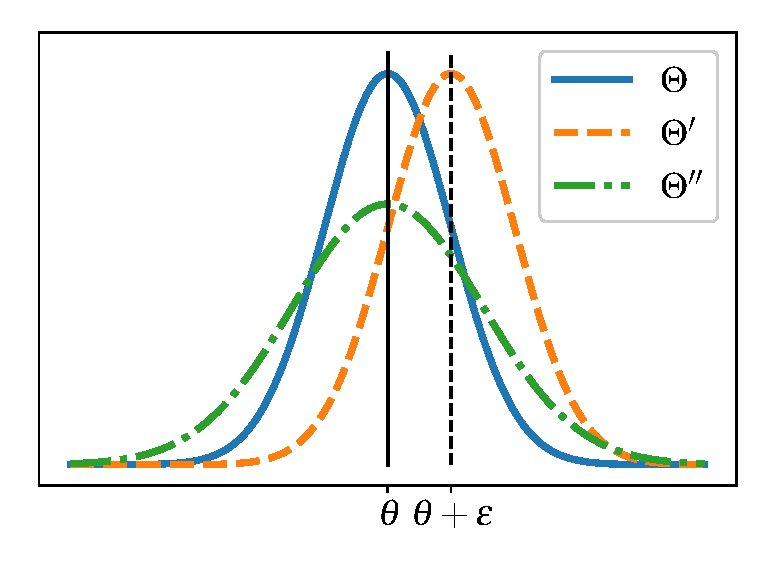
\includegraphics[width=0.5\textwidth]{figures/estimation/biais_variance}
  \caption{Distribution de 3 estimateurs de $\theta$.}
  \label{fig:biais_variance}
\end{figure}

\subsection{Exemple : Estimation non-biais�e de la variance}
Consid�rons $X$ est de carr� int�grable ($X \in \Lcal^2$), d'esp�rance $m$ et
de variance $\sigma^2$.

La \textbf{variance empirique} de $X$ est une variable al�atoire $S_n$, d�finie
par
\[
  S_n = \frac1n \sum_{i=1}^n (X_i - M_n)^2,
\]
o� $M_n$ est la moyenne empirique telle que d�finie pr�c�demment.

$S_n$ est un estimateur de $\sigma^2.$

Cependant, son biais vaut $\frac{n-1}{n} \sigma^2$  (voir calcul
  section~\ref{sec:estimation_proofs}).

On propose donc la \textbf{variance empirique corrig�e,} d�finie par 
\[
  S^*_n = \frac1{n-1} \sum_{i=1}^n (X_i - M_n)^2,
\]
et qui est non-biais�.

N�anmoins, le biais de la variance empirique tend vers 0 lorsque $n$ tend vers
$+\infty$. On parle alors d'un estimateur \textbf{asymptotiquement non-biais�.}

\subsection{Pr�cision d'un estimateur}
\label{sec:precision_estimateur}

Reprenons la figure~\ref{fig:biais_variance}. Les deux estimateurs $\Theta$ et
$\Theta^{\prime\prime}$ sont non-biais�s. Cependant, $\Theta^{\prime\prime}$ a
une plus grande variance ; une de ses r�alisation a une probabilit� plus grande
que pour $\Theta$ d'�tre �loign�e de $\theta$. 

C'est cette notion que l'on utilise pour mesurer la pr�cision d'un
estimateur. Dans le cas d'un estimateur non-biais�e, sa pr�cision est d�finie
comme sa variance.

Dans le cas g�n�ral d'un estimateur biais�, il faut aussi prendre en compte le
biais. Un estimateur biais� mais avec une faible variance pourra donner de
meilleures estimations (c'est-�-dire plus proches de la vraie valeur) qu'un
estimateur moins biais� mais avec une plus grande variance.

On utilise pour quantifier la pr�cision d'un estimateur ponctuel g�n�rique son
\textbf{erreur quadratique moyenne,} d�finie comme
\[
  \text{EQM}(\Theta_n) = \VV(\Theta_n) + \text{B}(\Theta_n)^2.
\]

\paragraph{Compromis biais-variance} Il est tout � fait possible qu'un
estimateur biais� ait une meilleure pr�cision qu'un estimateur non-biais�, si
ce dernier a une plus grande variance !

\subsection{Convergence d'un estimateur}
\label{sec:convergence_estimateur}

On utilise en anglais le terme de ``\textit{consistent}'', ce qui conduit les
francophones � parfois parler d'estimateur consistant plut�t que convergent.

\section{Estimation par maximum de vraisemblance}


\section{Calculs}
\label{sec:estimation_proofs}
\paragraph{Variance de la moyenne empirique} Soit $X$ une variable al�atoire
r�elle de carr� int�grable, d'esp�rance $m$ et de variance $\sigma^2$. Soient
$X_1, X_2, \dots, X_n$ ind�pendantes et identiquement distribu�es, de m�me loi
que $X$. 

Par d�finition de la variance, $\sigma^2 = \EE(X^2) - \EE(X)^2$ donc
$\EE(X^2) = \sigma^2 + m^2$.

Posons $M_n = \frac1n \sum_{i=1}^n X_i.$
\begin{align*}
  \VV(M_n) &= \EE(M_n^2) - \EE(M_n)^2 
   = \EE\left(\left(\frac1n \sum_{i=1}^n X_i\right)^2\right) - m^2 \\
  & = \frac1{n^2} \EE\left( \sum_{i=1}^n X_i \sum_{j=1}^n X_j\right) - m^2 \\
  & = \frac1{n^2} \EE\left( \sum_{i=1}^n \left(X_i^2 + \sum_{j \neq i }^n X_i X_j \right) \right) - m^2 \\
  & = \frac1{n} \left(\EE(X^2) + \sum_{j \neq i }^n \EE(X)^2 \right) - m^2 \\
  & = \frac1{n} \left(\sigma^2 + m^2 + (n-1) m^2  \right) - m^2 = \frac{\sigma^2}{n}.
\end{align*}

\paragraph{Biais de la variance empirique} Soit $X$ une variable al�atoire
r�elle de carr� int�grable, d'esp�rance $m$ et de variance $\sigma^2$. Soient
$X_1, X_2, \dots, X_n$ ind�pendantes et identiquement distribu�es, de m�me loi
que $X$. 

Posons $M_n = \frac1n \sum_{i=1}^n X_i$ et $S_n = \frac1n \sum_{i=1}^n (X_i - M_n)^2.$ Alors
\begin{align*}
  \EE(S_n) = \frac1n \sum_{i=1}^n \EE((X_i - M_n)^2)  & =  
    \frac1n \sum_{i=1}^n \left( \EE(X_i^2) +  \EE(M_n^2) - 2 \EE(X_i M_n) \right)  \\
  & = \EE(X^2) + \EE(M_n^2) - \frac2n \sum_{i=1}^n \EE(X_i M_n).
\end{align*}
Nous avons montr� lors du calcul de la variance de la moyenne empirique que
$\EE(X_i^2) = \sigma^2 + m^2$ et que $\EE(M_n^2) = m^2 + \frac{\sigma^2}{n}.$

De plus, par lin�arit� de l'esp�rance,
\[
  \EE(M_n^2) = \EE\left( \left(\frac1n \sum_{i=1}^n X_i \right) M_n \right) = \frac1n \sum_{i=1}^n \EE(X_i M_n),
\]
et donc 
\[
  \EE(M_n^2) - \frac2n \sum_{i=1}^n \EE(X_i M_n) = - \EE(M_n^2).
\]

On obtient ainsi 
\[
  \EE(S_n) = (\sigma^2 + m^2) - (m^2 + \frac{\sigma^2}{n}) = \frac{n-1}{n} \sigma^2.
\]
La variance empirique est donc biais�e et son biais vaut 
\[
  \text{B}(S_n) = \EE(S_n) - \sigma^2 = - \frac1n \sigma^2.
\]



\begin{plusloin}
\item Plus la variance d'un estimateur est faible, plus cet estimateur
  peut-�tre consid�r� comme pr�cis. Un estimateur est dit \textit{efficace}
  s'il est non-biais� et que sa variance tend vers la \textit{borne de
    Cram�r-Rao} quand la taille de l'�chantillon tend vers l'infini. La borne
  de Cram�r-Rao est une borne inf�rieure de la variance d'un estimateur,
  obtenue en prenant un point de vue de th�orie de l'information sur
  l'estimation statistique.
\end{plusloin}








\clearpage 

% \chapter{Tests d'hypoth�se}
% %-*- coding: iso-latin-1 -*-
\label{chap:tests}

\paragraph{Notions :} hypoth�se nulle, hypoth�se alternative, statistique de
test, p-valeur, tests multiples.
\paragraph{Objectifs p�dagogiques :} 
\begin{itemize}      
  \setlength{\itemsep}{3pt}
\item Reconna�tre une situation dans laquelle un test statistique est
  appropri�.
\item Poser les hypoth�ses de test nulle et alternative correspondant � un
  �nonc�.
\item Interpr�ter une statistique de test ou une p-valeur.
\end{itemize}


\section{Principe d'un test statistique}
\label{sec:principe_test}
Le but d'un test statistique est de d�terminer la fiabilit� d'une observation
faite sur une �chantillon.

\begin{exemple}
Si je lance une pi�ce 5 fois et obtiens 5 fois pile, puis-je en d�duire que
  la pi�ce est d�s�quilibr�e ? Ou ce r�sultat est-il d� au hasard de
  l'�chantillonnage ? Qu'en est-il si j'obtiens le m�me r�sultat apr�s 50
  lancers ? 
\end{exemple}

\textbf{Un test statistique permet de d�terminer si l'�chantillon observ�
  permet d'invalider une hypoth�se qu'il �tait raisonnable de formuler avant
  d'observer les donn�es.}

\begin{exemple}
  Reprenons l'exemple du lancer de pi�ce. Sous l'hypoth�se que la pi�ce est
  �quilibr�e, la probabilit� $\pi$ d'obtenir � pile � pour un lancer est $0,5$
  et celle d'obtenir pile pour 5 lancers est $0,5^5 = 3\%.$ Cette probabilit�
  est faible, mais non n�gligeable : on a 3\% de chance d'obtenir un r�sultat
  aussi extr�me que celui observ� sur un �chantillon.

  Pour 50 lancers, cette probabilit� tombe � $0,5^{50} = 9,10^{-16}.$ Cette
  probabilit� est extr�mement faible, et l'�chantillon ne soutient pas
  l'hypoth�se selon laquelle la pi�ce est �quilibr�e : nous pouvons la rejeter.
\end{exemple}

\section{Formalisme}
\label{sec:formalisme_test}
Soit $(X_1, X_2, \dots, X_n)$ un �chantillon al�atoire de taille $n \in \NN^*$
d'une variable al�atoire r�elle $X$ de loi $\PP_X.$ Rappelons que les
composantes $X_i$ de ce vecteur al�atoire sont ind�pendantes et identiquement
distribu�es, de m�me loi que $X$. Les notions pr�sent�es dans ce chapitre
s'appliquent aussi � des variables al�atoires de nature plus complexe (par
exemple, des valeurs al�atoires multi-dimensionnelles) mais nous nous limitons
aux variables al�atoires r�elles par souci de simplicit�.
Nous supposons aussi disposer d'un �chantillon $(x_1, x_2, \dots, x_n)$ qui est
une r�alisation de $(X_1, X_2, \dots, X_n)$.

Un test statistique repose sur les �l�ments suivants :
\begin{itemize}
\item Une \textbf{hypoth�se nulle,} not�e $\HH_0$. L'hypoth�se nulle est
  celle que l'on chercher � rejeter.
\item Une \textbf{hypoth�se alternative,} not�e $\HH_1$ ou $\HH_a$. C'est en
  g�n�ral la n�gation de $\HH_0$.
\item Une \textbf{statistique de test,} $T$, qui sert � mesurer � quel point un
  �chantillon � d�vie � de l'hypoth�se nulle.
\item Un \textbf{niveau de signification,} $0 < \alpha < 1$, qui est la
  probabilit� de rejeter l'hypoth�se nulle alors qu'elle est correcte. 
% qui sert �
  % d�terminer si la probabilit� d'observer, sous $\HH_0$, une statistique de
  % test au moins aussi extr�me que celle observ�e sur l'�chantillon
  % $(x_1, x_2, \dots, x_n)$ est suffisamment faible pour rejeter $\HH_0$.
\end{itemize}

Le but de cette section est de d�velopper ces notions.

\subsection{Hypoth�ses de test}
Conduire un test d'hypoth�se n�cessite de formuler deux hypoth�ses :
\begin{itemize}
\item Une \textbf{hypoth�se nulle,} not�e $\HH_0$. Cette hypoth�se doit �tre
  pr�cise et permettre de faire des calculs. Le but du test est de d�terminer
  s'il est raisonnable de rejeter cette hypoth�se.
\item Une \textbf{hypoth�se alternative,} not�e $\HH_1$ ou $\HH_a$. Cette
  hypoth�se est une forme de n�gation de $\HH_0$, et c'est l'hypoth�se que l'on
  adoptera si l'hypoth�se nulle est rejet�e.
\end{itemize}

L'hypoth�se nulle est souvent une hypoth�se formul�e sur la valeur d'un param�tre
$\theta \in \Scal \subseteq \RR$ caract�risant la loi $\PP_X$ de l'�chantillon
al�atoire. Il s'agit alors de tester
\begin{equation}
  \label{eq:h0}
  \HH_0: \theta = \theta_0,
\end{equation}
o� $\theta_0 \in \Scal$ est une valeur d�terministe fix�e � l'avance.

L'hypoth�se nulle peut cependant �tre de nature plus complexe, par exemple :
\begin{itemize}
\item � Deux variables statistique $X$ et $Y$ sont ind�pendantes � (c'est le
  cas du test d'ind�pendance du $\chi^2$ que nous verrons dans la PC1).
\item � Deux �chantillons $(x_1, x_2, \dots, x_n)$ et $(y_1, y_2, \dots, y_n)$
  sont des r�alisations de la m�me distribution � (c'est le cas du test de
  Wilcoxon-Mann-Whitney, qui d�passe le cadre de ce programme) ;
\end{itemize}

\paragraph{Pr�somption d'innocence} De m�me que le principe de la pr�somption
d'innocence veut que l'on recueille suffisamment de preuves pour rejeter
l'innocence, en th�orie des tests statistiques il y a pr�somption de
$\HH_0$. Il s'agit donc de savoir si l'�chantillon observ� (les preuves) est
suffisant pour rejeter $\HH_0$, ce dont on conclura $\HH_1.$ Par contre, si
l'on ne rejette pas $\HH_0$, cela peut venir soit de ce que $\HH_0$ est vraie,
soit de ce que nous n'avons pas suffisamment de donn�es pour rejeter
$\HH_0$. Ainsi, $\HH_0$ doit �tre une hypoth�se raisonnable, mais que l'on
aimerait avoir des raisons de r�futer.  

Dans le cadre d'une exp�rience scientifique, l'hypoth�se $\HH_0$ correspond
ainsi � l'�tat actuel des connaissances. Le but d'un test statistique est de
d�terminer si les donn�es qui semblent contredire cette hypoth�se sont
effectivement suffisamment improbables sous $\HH_0$ pour justifier de la
r�futer.
Dans le cadre d'un essai clinique, par exemple, l'hypoth�se $\HH_0$ se doit
d'�tre d�favorable au nouveau m�dicament (� le nouveau m�dicament est
inefficace � ou � le nouveau m�dicament n'est pas plus efficace que les
traitements connus �). Le but du test statistique est de d�terminer si les
donn�es r�colt�es jusqu'� pr�sent sont suffisantes pour r�futer cette
hypoth�se.

\begin{exemple}
  Dans le cas de notre lancer de pi�ce,
  \begin{itemize}
  \item $X$ est une variable al�atoire discr�te qui suit une loi de Bernoulli
    de param�tre $\pi$. $\PP_X(1) = \pi$ et $\PP_X(0) = 1-\pi$ ;
  \item l'�chantillon al�atoire est un vecteur $(X_1, X_2, \dots, X_n)$ de $n$
    composantes, iid de m�me loi que $X$ ;
  \item une s�rie de lancers est une r�alisation $(x_1, x_2, \dots, x_n)$ de ce
    vecteur al�atoire. Dans le cas de 5 lancers tous tombant sur � pile �,
    cet �chantillon est $(1, 1, 1, 1, 1)$ et $n=5.$
  \item l'hypoth�se nulle est $\HH_0: \pi = 0,5.$
  \end{itemize}
\end{exemple}

Dans le cas o� l'on cherche � tester la valeur d'un param�tre $\theta$ d'une
population, l'hypoth�se alternative peut prendre deux formes :
\begin{itemize}
\item $\theta \neq \theta_0$, ou en d'autres termes, 
  \begin{equation}
    \label{eq:h1_bilateral}
    \HH_1: \theta < \theta_0 \text{ ou } \theta > \theta_0.
  \end{equation}
  On parle alors de test \textbf{bilat�ral} (\textit{two-sided test} en
  anglais).
\item Si seulement l'une des deux parties de cette hypoth�se alternative nous
  int�resse, ou est possible, on parle de test \textbf{unilat�ral}
  (\textit{one-sided test} en anglais). Il s'agit alors de tester soit
  \begin{equation}
    \label{eq:h1_unilateral_gauche}
    \HH_1: \theta < \theta_0,
  \end{equation}
  soit
  \begin{equation}
    \label{eq:h1_unilateral_droite}
    \HH_1:  \theta > \theta_0.
  \end{equation}
\end{itemize}

De m�me que l'on �labore $\HH_0$ de sorte � ce qu'elle soit la plus plausible
avant d'avoir observ� les donn�es, on �labore $\HH_1$ en fonction de ce que
l'on esp�re d�couvrir. 

Reprenons l'exemple d'un essai clinique sur un nouveau m�dicament. Si
l'hypoth�se $\HH_0$ est � le nouveau m�dicament n'a pas d'effet �, on peut
poser l'hypoth�se alternative $\HH_1$ : � le nouveau traitement a un effet
positif sur l'�tat des patients �. On esp�re ici non seulement rejeter
l'hypoth�se nulle, mais aussi sugg�rer une efficacit� du traitement. Cette
hypoth�se est plus pr�cise que l'hypoth�se alternative selon laquelle � le
nouveau traitement a un effet sur l'�tat des patients �, cet effet pouvant �tre
n�gatif.

\begin{exemple}
  Dans le cas de notre lancer de pi�ce, l'hypoth�se alternative dans le cadre
  d'un test bilat�ral est
  \[
    \HH_1: \pi \neq 0,5.
  \]
  Si nous rejetons $\HH_0,$ notre conclusion sera que la pi�ce n'est pas �quilibr�e.

  Dans le cadre d'un test unilat�ral, par exemple
  \[
    \HH_1: \pi > 0,5,
  \]
  si nous rejetons $\HH_0,$ notre conclusion sera que la pi�ce n'est pas
  �quilibr�e, et qu'elle favorise � pile �.

  Il ne s'agit donc pas du m�me test.
\end{exemple}


\subsection{Statistique de test}
Une \textbf{statistique de test} $T$ est une statistique de l'�chantillon
al�atoire. Il s'agit donc d'une variable al�atoire r�elle, fonction de
$(X_1, X_2, \dots, X_n) : T = g(X_1, X_2, \dots, X_n)$ Cette statistique de
test sert � mesurer � quel point un �chantillon � d�vie � de l'hypoth�se nulle.

Une statistique de test est ainsi choisie de sorte � avoir une loi diff�rente
sous $\HH_0$ et sous $\HH_1$, et de sorte � ce que sa loi sous $\HH_0$ soit
connue : c'est ce qui permettra de d�terminer un crit�re de rejet de $\HH_0$
garantissant le niveau de signification choisi.

La plupart des test statistiques reposent sur des statistiques de test dont le
d�veloppement a �t� long et minutieux. Le choix entre plusieurs statistiques
candidates pour un m�me probl�me est un choix difficile, qui repose entre
autres sur la validit� des hypoth�ses sur la distribution de l'�chantillon
al�atoire ou sur sa taille qui permettent de d�terminer sa loi sous $\HH_0$.

\paragraph{Remarque} Pour des tests portant sur un param�tre
($\HH_0: \theta = \theta_0$), la statistique de test est souvent bas�e sur la
diff�rence entre un estimateur de ce param�tre et sa valeur sous $\HH_0$.

\begin{exemple}
  Reprenons l'exemple du lancer de pi�ce.

  Dans la section~\ref{sec:principe_test}, nous avons choisi comme statistique
  de test $T$ le nombre de pile obtenus dans l'�chantillon :
  \[
    T = \sum_{i=1}^n X_i.
  \]

  Sous $\HH_0$, autrement dit si $\pi=0,5$, la loi de $T$ est d�termin�e par 
  \[
    \PP(T=k) = \PP\left(\sum_{i=1}^n X_i = k\right) \text{ pour } k=0, 1,
    \dots, n.
  \]
  On reconnait ici une loi binomiale de param�tres $n$ et $\pi.$
\end{exemple}


\subsection{Niveau de signification}
Nous avons maintenant pos� $\HH_0$, $\HH_1$, et une statistique de test $T$
dont nous connaissons la loi $\PP_{T0}$ sous $\HH_0$. Il nous faut maintenant
d�terminer le \textbf{domaine de rejet} du test, autrement dit l'ensemble
$\Ical \subseteq \RR$ de ses valeurs qui conduisent � rejeter $\HH_0$.

Pour ce faire, nous avons besoin de fixer le \textbf{niveau de signification}
(\textit{significance level}), $0 < \alpha < 1$, qui est la probabilit� de
rejeter l'hypoth�se nulle alors qu'elle est correcte. Ce seuil est fix� �
l'avance, g�n�ralement parmi $\alpha = 1\%$, $\alpha = 5\%$ ou $\alpha = 10\%$,
et d�termine � quel point le test est strict.

Ainsi, il s'agit de d�terminer $\Ical \subseteq \RR$ de sorte � ce que
$\PP_{T0}(T \in \Ical) = \alpha.$

\begin{exemple}
  Dans l'exemple du lancer de pi�ce, nous avons choisi le nombre de pile comme
  statistique de test $T$. Sous $\HH_0 : \pi = 0,5$, $T$ suit une loi binomiale
  de param�tres $n$ (le nombre de lancers) et $\pi$.

  Posons $\alpha = 5\%.$

  Consid�rons le test unilat�ral $\HH_1 : \pi > 0,5$. Si nous rejetons $\HH_0$,
  nous en conclurons que la pi�ce est biais�e en faveur du c�t� pile. Cela
  signifie que nous souhaitons rejeter $\HH_0$ quand le nombre de pile dans
  l'�chantillon est grand. Il est ici naturel de consid�rer un domaine de rejet
  de la forme $\Ical = \mathopen]t_0, n\mathclose].$ En d'autres termes, nous
  allons rejeter $\HH_0$ si la r�alisation $t$ de $T$ sur notre �chantillon est
  plus grande qu'un seuil $t_0,$ fix� tel que $\PP_{T0}(T > t_0) = \alpha.$

  En d'autres termes, si $F_{T0}$ est la fonction de r�partition de $T$ sous
  $\HH_0$, $t_0$ est fix� de sorte � ce que $F_{T0}(t_0) = \alpha$. Dans notre
  exemple avec $n=5$ et $\alpha=0,05$, cela fixe $t_0 = 4.$

  Le test consiste donc � rejeter l'hypoth�se nulle si tous les 5 lancers
  aboutissent � pile.

  Consid�rons maintenant le test unilat�ral $\HH_1 : \pi < 0,5.$ Rejeter
  $\HH_0$ conduit � conclure que la pi�ce est biais�e en faveur du c�t�
  face. Nous consid�rons maintenant un domaine de rejet de la forme
  $\Ical = \mathopen[0, t_0 \mathclose[,$ et $t_0$ est d�termin� par
  $\PP_{T0}(T < t_0) = \alpha.$ Avec $n=5$ et $\alpha=0,05$, cela fixe
  $t_0=1$. Le test consiste donc � rejeter l'hypoth�se nulle si aucun des 5
  lancers n'aboutit � pile.

  Enfin, consid�rons le test bilat�ral $\HH_1 : \pi \neq 0,5.$ Rejeter $\HH_0$
  conduit � conclure que la pi�ce est biais�e, en faveur de l'un ou de l'autre
  de ses c�t�s. Nous consid�rons alors un domaine de rejet de la forme
  $\Ical = \mathopen[0, t_l \mathclose[ \; \cup \; \mathopen]t_r, n
  \mathclose].$
  Il nous faut donc choisir $t_l$ et $t_r$ de sorte � ce que
  $\PP_{T0}(T < t_l) + \PP_{T0}(T > t_r) = \alpha.$ Il est assez naturel de
  fixer alors $\PP_{T0}(T < t_l) = \PP_{T0}(T > t_r) = \frac{\alpha}{2}.$ Avec
  $n=5$ et $\alpha=0,05$, on obtient $t_l = 0$ et $t_r = 5$ et il n'est donc
  jamais possible de rejeter l'hypoth�se nulle.

  Le test que nous venons de d�finir s'appelle le \textbf{test binomial.}

  \paragraph{Remarque importante} On observe ici que, parmi les trois
  hypoth�ses alternatives envisag�es, seul le test statistique unilat�ral
  $\HH_1: \pi > 0,5$ nous permet de rejeter l'hypoth�se nulle. C'est une
  observation g�n�rale : un test unilat�ral est plus puissant qu'un test
  bilat�ral ; cependant il n'est utile que si on sait de quel c�t� le d�finir.
\end{exemple}

\subsection{Valeur critique}
Dans le cas d'un test sur la valeur d'un param�tre $\theta$, c'est-�-dire avec
pour hypoth�se nulle 
\[
  \HH_0: \theta = \theta_0,
\]
le domaine de rejet sera de la forme
\begin{itemize}
\item $\Ical = \mathopen]t_r, +\infty \mathclose[$ pour le test unilat�ral �
  droite, pour lequel $\HH_1 : \theta > \theta_0$ ;
\item $\Ical = \mathopen]-\infty, t_l \mathclose[$ pour le test unilat�ral �
  gauche, pour lequel $\HH_1 : \theta > \theta_0$ ;
\item
  $\Ical = \mathopen]-\infty, t_l \mathclose[ \cup \mathopen]t_r, +\infty
  \mathclose[$
  pour le test bilat�ral, pour lequel $\HH_1 : \theta \neq \theta_0$.
\end{itemize}

On cherchera souvent � utiliser une statistique de test symm�trique, de sorte �
pouvoir utiliser $t_r = - t_l$.  Dans ce cas $t_0 = t_r$ est appel�e
\textbf{valeur critique} du test et est telle que
\begin{itemize}
\item $\PP_{T0}(T > t_0) = \alpha$ pour le test unilat�ral � droite ; 
\item $\PP_{T0}(T < - t_0) = \alpha$ pour le test unilat�ral � gauche ; 
\item $\PP_{T0}(|T| > t_0) = \alpha$ pour le test bilat�ral. 
\end{itemize}

\subsection{p-valeur}
La \textbf{p-valeur} (\textit{p-value} en anglais) d'un test statistique est
d�finie dans le cas o� le test statistique peut �tre r�alis� en comparant une
statistique de test $T$\footnote{ou sa valeur absolue $\abs{T}$, sans perte de
  g�n�ralit�, puisque l'on peut alors utiliser la statistique $U = \abs{T}.$} �
une valeur critique $t_0$.

Dans ce contexte, �tant donn� un �chantillon $(x_1, x_2, \dots, x_n)$ et la
r�alisation $t$ de $T$ sur cet �chantillon, on appelle \textbf{p-valeur} la
probabilit� $\PP_{T0}(T > t)$ pour un test unilat�ral � droite (respectivement,
$\PP_{T0}(T < -t)$ pour un test unilat�ral � gauche, et $\PP_{T0}(\abs{T} > t)$
pour un test bilat�ral). 

L'hypoth�se nulle est rejet�e si la p-valeur est plus petite que le niveau de
signification. On dit alors que la p-valeur est \textbf{significative.}

En d'autres termes, la p-valeur peut �tre interpr�t�e comme la probabilit�
d'obtenir, sous l'hypoth�se nulle, un r�sultat au moins aussi extr�me que celui
observ�.

On rapporte ainsi g�n�ralement comme r�sultat d'un test non pas la statistique
de test r�alis�e sur l'�chantillon observ�, mais la p-valeur correspondante.

On lira ainsi dans des publications scientifiques des assertions suivies de �
($p < 0,05$) �, signifiant que l'assertion en question est l'hypoth�se
alternative d'un test dont l'hypoth�se nulle a �t� rejet�e avec une p-valeur
inf�rieure � $5\%.$

\newpage
\begin{exemple}
  Le test que nous avons d�fini dans l'exemple de la pi�ce de monnaie s'appelle
  le test binomial. Il est impl�ment� dans \texttt{scipy.stats} :
  \begin{lstlisting}[language=Python]
    t = 5 # nb pile 
    n = 5 # taille �chantillons 
    pi = 0.5 
    import scipy.stats as st 
    st.binom_test(t, n, pi, alternative='greater') # unilat�ral � droite
  \end{lstlisting}
\end{exemple}

\begin{attention}
  On fera attention � ne pas sur-interpr�ter la p-valeur. En particulier, la
  p-valeur \textit{n'est pas} la probabilit� que l'hypoth�se nulle soit vraie :
  $\PP(t|\HH_0) \neq \PP(\HH_0|t)$.
\end{attention}


\subsection{Erreurs de premi�re et deuxi�me esp�ce}
\label{sec:test_errors}
Deux types d'erreurs sont possibles quand on fait un test d'hypoth�se :
\begin{itemize}
\item Rejeter l'hypoth�se nulle alors qu'elle est correcte : on parle d'une
  \textbf{erreur de premi�re esp�ce}, ou \textbf{erreur de Type I}
  (\textit{Type I error} en anglais).
\item Accepter l'hypoth�se nulle alors qu'elle est en fait fausse : on parle
  d'une \textbf{erreur de deuxi�me esp�ce}, ou \textbf{erreur de Type II}
  (\textit{Type II error} en anglais).
\end{itemize}

\paragraph{Moyen mn�motechnique} Ces deux types d'erreurs sont num�rot�s dans
le m�me ordre que dans l'histoire du gar�on qui criait au loup : d'abord les
villageois pensaient qu'il y avait un loup alors qu'il n'y en avait pas (erreur
de premi�re esp�ce), mais � la fin les villageois pensaient qu'il n'y avait pas
de loup alors qu'il y en avait un (erreur de deuxi�me esp�ce). Ici, l'hypoth�se
nulle est l'hypoth�se correspondant � l'�tat � par d�faut � du village, �
savoir sans loup\footnote{Les fans de \textit{Battlestar Galactica} pourront
construire leur propre moyen mn�motechnique � partir de Starbuck qui refuse
de faire valider les �l�ves pilotes apr�s avoir fait valider Zak.}.

Le niveau de signification $\alpha$ est ainsi la probabilit� de commettre une
erreur de premi�re esp�ce.

La probabilit� de commettre une erreur de deuxi�me esp�ce est g�n�ralement not�
$\beta$. La probabilit� de rejeter $\HH_0$ � raison, $1-\beta$, est appel�e la
\textbf{puissance} du test (\textit{power} en anglais).


\section{Comparaison d'une moyenne observ�e � une moyenne th�orique}
\label{sec:test_moyenne}
Dans cette section, nous allons d�rouler un autre exemple de test statistique. 

Nous souhaitons tester l'hypoth�se selon laquelle les pigeons du Jardin du
Luxembourg ont un poids moyen de 300g. Nous disposons de mesures pour 40
pigeons, captur�s et pes�s par des �l�ves de l'�cole, dont la moyenne est de
312g et l'�cart-type 31g.

D�finissons une variable al�atoire r�elle $X$ de carr� int�grable. $X$ mod�lise
le poids d'un pigeon. Posons $\mu$ l'esp�rance de $X$ et $\sigma^2$ sa
variance.

\subsection{Hypoth�ses de test}
\paragraph{Question:} Comment mod�liser ce probl�me ? Que poser pour $\HH_0$ et
$\HH_1$ ?
\begin{answer}
  Nous posons $n=40$ ; les poids des 40 pigeons, $(x_1, x_2, \dots, x_n)$, sont
  la r�alisation de l'�chantillon al�atoire $(X_1, X_2, \dots, X_n)$ compos� de
  variables al�atoires ind�pendantes et identiquement distribu�es de m�me loi
  que $X$.

  Nous posons l'hypoth�se nulle � tester
  \[
    \HH_0 : \mu = \mu_0,
  \]
  avec $\mu_0 = 300\si{g}.$

  Nous n'avons aucun a priori sur le poids des pigeons du Jardin du Luxembourg,
  et formulons donc l'hypoth�se alternative bilat�rale
  \[
    \HH_1 : \mu \neq \mu_0.
  \]
\end{answer}

\subsection{Statistique de test}
Pour tester $\HH_0$, nous souhaitons d�terminer la probabilit� d'observer une
moyenne empirique $\hatm$ de 312g si l'esp�rance de $X$ est de 300g.  En
posant $M_n$ la moyenne empirique de l'�chantillon, nous souhaitons d�terminer
$\PP(M_n=\hatm|\mu=\mu_0)$.

Le th�or�me central limite nous indique que 
\[
  \frac{\sqrt{n} (M_n - \mu)}{\sigma}  \cvloi \Ncal(0, 1).
\]

Avec $n = 40$, nous pouvons supposer que cette limite est suffisamment proche
d'�tre atteinte pour poser
\[
  \frac{\sqrt{n} (M_n - \mu)}{\sigma}  \sim \Ncal(0, 1).
\]

Nous ne connaissons pas la variance $\sigma^2$ de $X$ ; cependant nous pouvons
l'estimer gr�ce � l'�cart-type empirique $\hatsigma = 31\si{g},$ et utiliser 
\begin{equation}
  \frac{\sqrt{n} (M_n - \mu)}{\hatsigma}  \sim \Ncal(0, 1).
\label{eq:tcl_moyenne}
\end{equation}
Nous ne rempla�ons pas $\mu$ par son estimation $\hatm$ : ce n'aurait aucun
sens, car nous cherchons justement � tester sa valeur.

\paragraph{Question :} Comment utiliser l'�quation~\eqref{eq:tcl_moyenne} pour
d�finir une statistique de test ?
\begin{answer}
  Si $\HH_0$ est vraie, alors $\mu = \mu_0$ et la variable al�atoire r�elle
  \begin{equation}
    \label{eq:z_moyennes}
    Z = \frac{\sqrt{n} (M_n - \mu_0)}{\hatsigma}
  \end{equation}
  est une gaussienne standard : $Z \sim \Ncal(0, 1)$.

  $Z$ est donc une variable al�atoire r�elle dont nous connaissons la
  distribution sous l'hypoth�se nulle. Cela en fait une bonne candidate � �tre
  statistique de test.
\end{answer}
Sous $\HH_0$, on s'attend � ce que la r�alisation de $Z$ sur l'�chantillon
observ� soit proche de $0.$ Nous r�alisons un test bilat�ral et n'avons aucun a
priori sur le signe de $Z.$ Ainsi, nous rejetterons $\HH_0$ si la r�alisation
de $\abs{Z}$ est � trop grande � pour �tre plausible.

Le test statistique permettant de tester si la moyenne d'un �chantillon vaut
une valeur pr�d�termin�e consiste donc � rejeter $\HH_0$ si $\abs{Z} > z_0.$

\paragraph{Question : } �tant donn� un niveau de signification $\alpha$, quelle
est la valeur critique $z_0$ ?
\begin{answer}
  Nous souhaitons que la probabilit� de rejeter $\HH_0$ alors qu'elle est vraie
  soit �gale � $\alpha.$ En d'autres termes, nous cherchons $z_0$ tel que
  \[
    \PP(\abs{Z} > z_0) = \alpha, \text{ sachant } Z \sim \Ncal(0, 1).
  \]
  La densit� de $Z$ �tant symm�trique, on cherche donc $z_0$ telle que 
  \[
    \PP(Z < -z_0) = \frac{\alpha}{2}.
  \]
  Ceci est illustr� sur la figure~\ref{fig:z_moyenne}.  
\end{answer}

\begin{figure}[h]
  \centering
  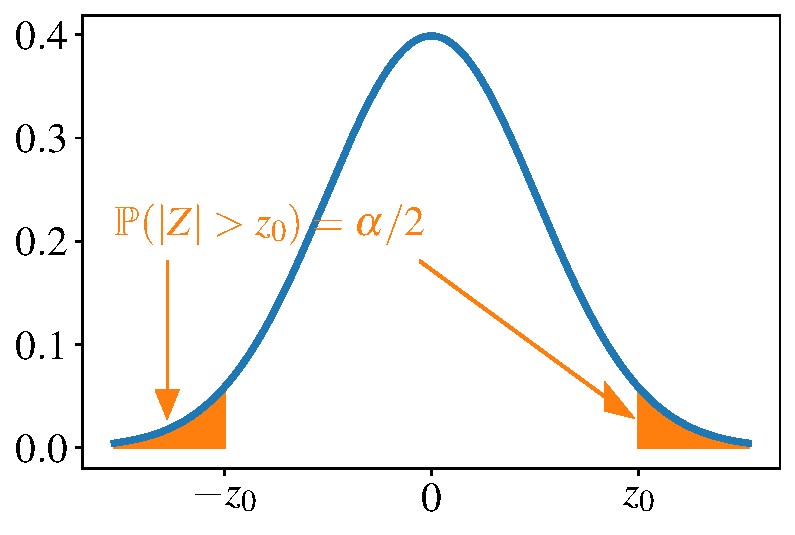
\includegraphics[width=0.5\textwidth]{figures/tests/z_moyenne}
  \caption{Densit� d'une gaussienne centr�e r�duite. L'aire color�e vaut
    $\alpha$ et correspond au domaine de rejet du test.}
  \label{fig:z_moyenne}
\end{figure}

\paragraph{Question :} Peut-on rejeter l'hypoth�se selon laquelle les pigeons
du jardin du Luxembourg ont un poids moyen de 300g ?
\begin{answer}
  Cela d�pend du niveau de signification que l'on choisit.

  Calculons tout d'abord la r�alisation de la statistique de test $Z$ sur notre
  �chantillon : $z = 2,45.$

  Posons $\alpha = 0,05.$ Alors $z_0 \approx 1,96.$ On a bien $z > z_0$ et on
  rejette l'hypoth�se nulle. On dit que l'�cart entre $M_n$ et $\mu_0$ est
  \textbf{statistiquement significatif.}

  Posons maintenant $\alpha = 0,01.$ Le domaine de rejet est plus restreint ;
  $z_0 \approx 2,58.$ On ne peut pas rejeter l'hypoth�se nulle. L'�cart entre
  $M_n$ et $\mu_0$ n'est pas statistiquement significatif.


  Cet exemple est illustr� sur la figure~\ref{fig:z_pigeons}.
\end{answer}


\begin{figure}[h]
  \centering
  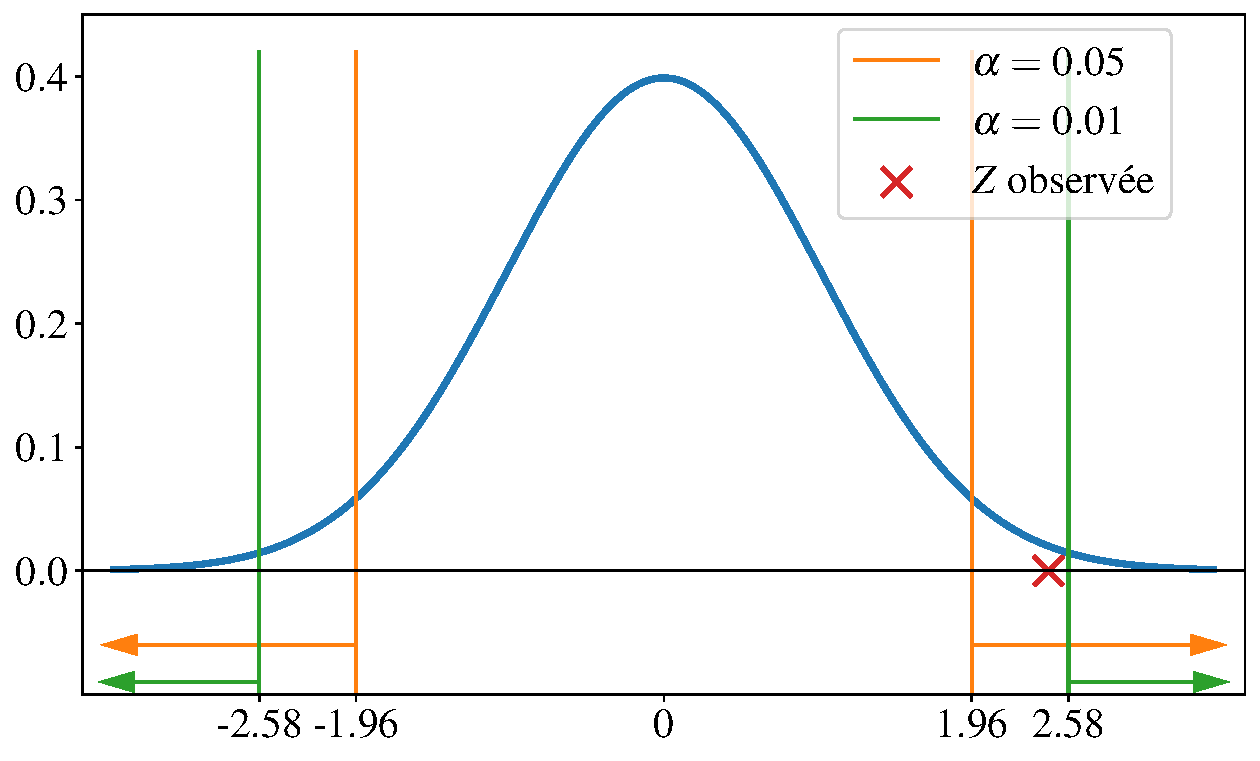
\includegraphics[width=0.65\textwidth]{figures/tests/z_pigeons}
  \caption{Densit� d'une gaussienne centr�e r�duite. La valeur $z=2,45$ est
    dans le domaine de rejet pour $\alpha = 0,05$ mais pas pour
    $\alpha = 0,01$.}
  \label{fig:z_pigeons}
\end{figure}

\subsection{p-valeur}
\paragraph{Question :} Quelle est la p-valeur correspondant � la valeur de test
$z=2,45$ ?
\begin{answer}
  La p-valeur est
  \[
    \PP(\abs{Z}) \geq \abs{z} = \PP(Z \leq -\abs{z}) + \PP(Z \geq \abs{z}) = 2
    \PP(Z \leq -\abs{z}) = 2 \Phi(-\abs{z}) = 0,018.
  \]
  o� $\Phi$ est la fonction de r�partition d'une gaussienne standard.

  Cette p-valeur est bien inf�rieure au seuil de signification $\alpha = 0,05$,
  mais sup�rieure au seuil de signification $\alpha = 0,01$.
\end{answer}

\subsection{Test unilat�ral � droite}
Supposons maintenant que nous nous demandons si les pigeons du Jardin du
Luxembourg, qui nous semblent particuli�rement bien nourris de restes des
sandwicheries environnantes, ne seraient pas plus lourds que la moyenne de
300g. Il s'agit maintenant de faire un test unilat�ral � droite, pour lequel
\[
  \HH_1 : \mu > \mu_0.
\]

\paragraph{Question :} Comment cela transforme-t-il notre test d'hypoth�se ?
\begin{answer}
  Le test statistique consiste maintenant � rejeter $\HH_0$ si $Z > z_r$ (sans
  valeur absolue). En particulier, toutes les valeurs n�gatives nous font
  accepter $\HH_0$, contrairement au cas bilat�ral.
  
  La valeur critique $z_r$ est telle que 
  \[
    \PP(Z > z_r) = \alpha, \text{ sachant } Z \sim \Ncal(0, 1).
  \]
  La densit� de $Z$ �tant symm�trique, on cherche donc $z_0$ telle que 
  \[
    \Phi(-z_r) = \alpha.
  \]
  
  Pour $\alpha = 0,05,$ la valeur critique est $z_r = 1,64.$ Pour
  $\alpha = 0,01,$ la valeur critique est $z_r = 2,33.$ L'hypoth�se nulle est
  rejet�e dans les deux cas.

  Le test unilat�ral est plus puissant pour les valeurs du bon c�t�.

  Cet exemple est illustr� sur la figure~\ref{fig:z_pigeons_unilateral}.
\end{answer}


\begin{figure}[h]
  \centering
  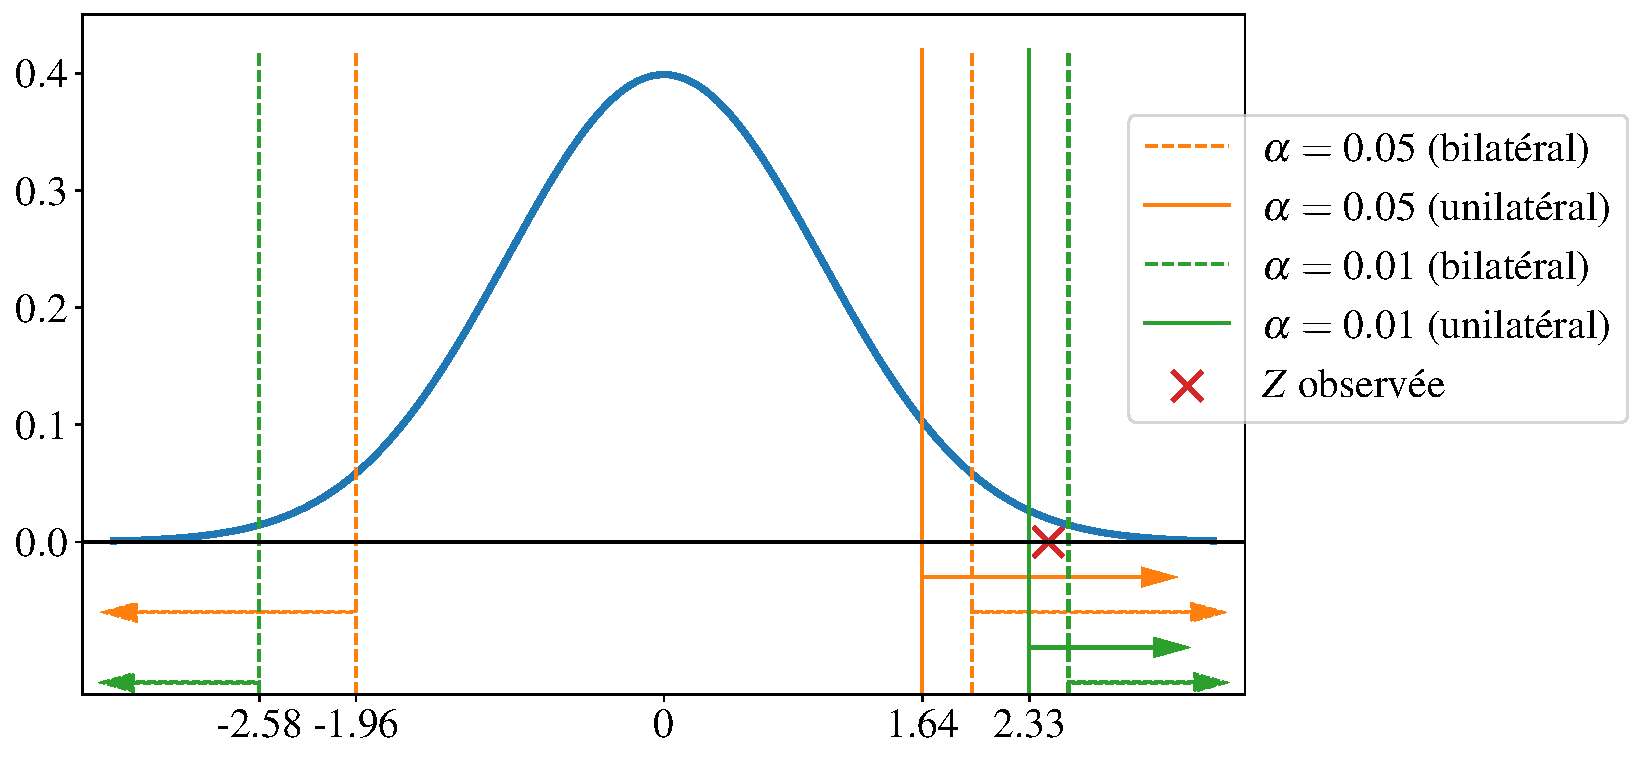
\includegraphics[width=0.85\textwidth]{figures/tests/z_pigeons_unilateral}
  \caption{Densit� d'une gaussienne centr�e r�duite. La valeur $z=2,45$ est
    dans le domaine de rejet pour $\alpha = 0,05$ et pour $\alpha = 0,01$ dans
    le cas du test unilat�ral.}
  \label{fig:z_pigeons_unilateral}
\end{figure}

\subsection{Intervalle de confiance $\bigstar$}
\label{sec:ic}
Reprenons le test bilat�ral.

�tant donn� $\alpha,$ nous avons d�termin� $z_0$ de sorte � ce que
\[
  \PP(\abs{Z} > z_0) = \alpha, \text{ sachant } Z \sim \Ncal(0, 1).
\]

En d'autres termes, 
\[
  \PP(-z_0 \leq Z \leq z_0) = 1 - \alpha. 
\]
(On pourra se r�f�rer � la figure~\ref{fig:z_moyenne}.)

D'apr�s la d�finition de $Z$ (�quation~\eqref{eq:z_moyennes}), cela est �quivalent � 
\[
  \PP\left( M_n - \frac{\hatsigma}{\sqrt{n}} z_0 \leq 
    \mu \leq M_n + \frac{\hatsigma}{\sqrt{n}}z_0 \right) = 1 - \alpha.
\]

Ainsi l'intervalle 
\[
  \left[ M_n - \frac{\hatsigma}{\sqrt{n}} z_0, \; M_n +
    \frac{\hatsigma}{\sqrt{n}} z_0 \right]
\]
est un \textbf{intervalle de confiance} � $(1 - \alpha)$ pour la taille moyenne
$\mu$ (voir Probabilit�s V).

Dans notre exemple, l'intervalle de confiance � 95\% pour la valeur moyenne du
poids d'un pigeon est $[302,4\si{g}~; 321,6\si{g}]$.
$\mu_0 = 300\si{g}$ n'est pas dans l'intervalle de confiance ; on adopte l'hypoth�se
alternative selon laquelle $\mu \neq \mu_0.$

L'intervalle de confiance � 99\% est $[299,4\si{g}~; 324,6\si{g}].$ Cet
intervalle contient $\mu_0$. On ne peut pas rejeter l'hypoth�se nulle.

\paragraph{Exercice :} Calculer l'intervalle de confiance � 95\% et � 99\% pour
le test d'hypoth�se unilat�ral � droite. (Solution : cf section~\ref{sec:ic_sol}.)
% \section{Test d'ind�pendance du $\chi^2$}
% \label{sec:chi2}

\subsection{Tests de comparaison de moyenne $\bigstar$} 
Le test que nous avons �tudi� dans cette section, qui permet de comparer la
moyenne d'un �chantillon suffisamment large pour �tre dans la limite du
th�or�me centrale limite ($n \geq 30$) � sa moyenne th�orique, s'appelle un
\textbf{test Z}, ou \textit{Z-test} en anglais, par r�f�rence � la notation $Z$
couramment utilis�e pour une variable normalement distribu�e de moyenne 0 et
variance 1.

Dans le cas d'un �chantillon de faible taille, le th�or�me central limite ne
s'applique pas. Si l'on suppose $X$ normalement distribu�e, on peut alors
appliquer un test de Student, ou test t (\textit{t-test} en anglais), ainsi
appel� car la statistique de test suit une loi de Student.

Des variantes de ces tests Z et t peuvent aussi �tre utilis�s pour comparer les
moyennes de deux �chantillons, appari�s ou non. On dit que deux �chantillons
al�atoires $(X_1, X_2, \dots, X_n)$ et $(Y_1, Y_2, \dots, Y_n)$ sont appari�s
quand les variables $X_i$ et $Y_i$ d�crivent le m�me individu $i$. Il peut par
exemple s'agir de mesures r�p�t�es sur les m�mes individus, soit prises par
deux appareils diff�rents, soit prises avant et apr�s un traitement.



\section{Tests d'hypoth�ses multiples}
\label{sec:mht}
\paragraph{Question} Imaginons l'exp�rience de pile ou face suivante : je lance
15 fois une pi�ce �quilibr�e, et demande � une personne en face de moi de
pr�dire avant chaque lancer si je vais obtenir pile ou face. Supposons que
cette personne me donne la bonne r�ponse 12 fois. A-t-elle un don de voyance ?
\begin{answer}
  Pour r�pondre � cette question, posons $X$ une variable de Bernouilli de
  param�tre $p$ mod�lisant, pour un lancer de pi�ce, le succ�s de la personne :
  $X$ vaut 0 si la personne n'a pas donn� la bonne pr�diction et 1
  sinon. L'hypoth�se nulle est
  \[
    \HH_o : p = 0,5 \text{ (la personne n'a pas de don de voyance)}.
  \]
  Nous pouvons ici poser une hypoth�se alternative unilat�rale � droite :
  \[
    \HH_1 : p > 0,5 \text{ (la personne a un don de voyance)}.
  \]
  Il s'agit du test binomial que nous avons d�fini dans la
  section~\ref{sec:formalisme_test}, mais ici la variable mod�lise non pas le
  r�sultat du lancer de pi�ce mais la correction de la r�ponse donn�e par mon
  cobaye.

  La statistique de test $T$ est le nombre de succ�s dans l'�chantillon. Sous
  $\HH_0$, $T \sim \Bcal(n, p).$ La p-valeur correspondant � 12 succ�s est donc
  $\PP_{\HH_0}(T \geq 12) = 1 - \PP(T \leq 11) = 0,018$. Cette p-valeur est
  significative pour $\alpha = 5\%$.
\end{answer}

\paragraph{Question} Supposons maintenant que je fasse ce test avec toute la
classe. Vous �tes derri�re votre ordinateur et ne communiquez pas entre
vous. Trois �l�ves passent mon test de pyschisme, autrement dit tombent juste
au moins 12 fois sur 15. Dois-je appeler la presse ?
\begin{answer}
  Supposons une promo de $m=125$ �l�ves. Nous posons maintenant $Y$ une
  variable de Bernouilli de param�tre $\pi$ mod�lisant le succ�s d'une personne
  sur 15 lancers. Nous faisons ici un nouveau test statistique sur $Y$,
  \[
    \HH_0^\prime : \pi = 0,018 \text { \qquad et \qquad} \HH_1^\prime : \pi >
    0,018.
  \]
  Il s'agit toujours d'un test binomial. La statistique de test $U$ est le
  nombre d'�l�ves passant le test. Sous $\HH_0^\prime$, $U \sim \Bcal(m,
  \pi)$.
  La p-valeur est ici
  $\PP_{\HH_0^\prime}(T \geq 3) = 1 - \PP(T \leq 2) = 0,39.$ Cette p-valeur
  n'est pas significative !
\end{answer}

Cet exemple illustre le principe suivant : plus on fait de tests, et plus on a
de chances de voir appara�tre une p-valeur significative. 

Il est n�cessaire de corriger cet effet : on parle de \textbf{correction} ou
\textbf{ajustement de tests d'hypoth�se multiples.} La plus simple et plus
utilis�es de ces corrections, propos�e par la biostatisticienne Olive Jean
Dunn, est connue sous le nom de \textbf{correction de Bonferroni} : il s'agit
simplement de diviser le niveau de signification par le nombre de tests
\[
  \alpha \leftarrow \frac{\alpha}{m}.
\]

Cette correction se justifie de la fa�on suivante : notons
$p_1, p_2, \dots, p_m$ les p-valeurs obtenue pour $m$ tests, testant chacun
$\HH_0$ vs. $\HH_1$, et supposons que $\HH_0$ est
vraie pour les $m_0$ premiers tests . Alors 
\[
  \PP\left(\bigcup_{i=1}^{m_0} \left( p_i \leq \frac{\alpha}{m} \right)\right)  \leq
  \sum_{i=1}^{m_0} \PP \left( p_i \leq \frac{\alpha}{m} \right)= \frac{m_0
    \alpha}{m} \leq \alpha.
\]



\section{Compl�ments}
\subsection{Solution de l'exercice section~\ref{sec:ic} $\bigstar$}
\label{sec:ic_sol}
Nous avons d�termin� la valeur critique $z_r$ de sorte � ce que 
  \[
    \PP(Z \leq z_r) = 1-\alpha.
  \]

Comme $Z = \frac{\sqrt{n} (M_n - \mu_0)}{\hatsigma}$, cela est �quivalent � 
\[
  \PP \left(\mu \geq M_n - \frac{\hatsigma}{\sqrt{n}} z_r \right) = 1 - \alpha.
\]

Ainsi l'intervalle 
\[
  \left[M_n - \frac{\hatsigma}{\sqrt{n}} z_r, +\infty \right]
\]
 est un intervalle de confiance unilat�ral � $(1-\alpha)$ pour la taille moyenne $\mu$.

 Dans notre exemple, l'intervalle de confiance unilat�ral � droite � 95\% pour
 la valeur moyenne du poids d'un pigeon est $[303,9\si{g}, +\infty]$. Cet
 intervalle contient $\mu_0$ et on ne peut pas rejeter l'hypoth�se nulle.  �
 99\%, cet intervalle est $[300,6\si{g}, +\infty[.$ Ces r�sultats sont
 coh�rents.

\begin{plusloin}
\item On dit d'un test statistique qu'il est sans biais si sa puissance est
  sup�rieure au niveau de signification : $1 - \beta > \alpha$.
\item On dit d'un test statistique qu'il converge si la suite des erreurs de
  deuxi�me esp�ce converge vers $0$ : $1 - \beta \cvn 0.$ 
\item Pour plus de d�tails sur la sur-interpr�tation des p-valeurs en sciences
  et le \textit{p-hacking} (consistant � ne conserver, parmi de nombreux tests
  conduits sur les donn�es, ceux qui donnent des p-valeurs significatives), on
  pourra se reporter aux r�f�rences suivantes.
  \vspace{-105pt}
  \begin{thebibliography}{99}
  \bibitem{ioannidis2005}
    John PA Ioannidis.
    {Why most published research findings are false.}
    \textit{PLoS medicine,} 
    2(8):{e124},
    {2005.}

  \bibitem{head2015}
    Megan L Head, Luke Holman, Rob Lanfear, Andrew T Kahn and Michael D Jennions.
    {The extent and consequences of p-hacking in science.}
    \textit{PLoS biology},
    13(3):{e1002106},
    {2015.}
  \bibitem{wasserstein2016}
    Ronald L Wasserstein, Nicole A Lazar, et al.
    {The ASA's statement on p-values: context, process, and purpose}.
    \textit{The American Statistician},
    70(2):129--133,
    2016.

  \bibitem{holmes2018}
    Susan Holmes.
    {Statistical proof? The problem of irreproducibility}.
    \textit{Bulletin (New Series) of the American Mathematical Society},
    {55}(1), 2018.
  \end{thebibliography}
\end{plusloin}


%%% Local Variables:
%%% mode: latex
%%% TeX-master: "sdd_2020_poly"
%%% End:

% \part{Analyse exploratoire}
% \chapter{R�duction de dimension}
% %-*- coding: iso-latin-1 -*-
\label{chap:dimred}

\paragraph{Notions :} s�lection de variables ; extraction de variables ;
 analyse en composantes principales ; analyse en composantes principales probabiliste.
\paragraph{Objectifs p�dagogiques :} 
\begin{itemize}      
  \setlength{\itemsep}{3pt}
\item Expliquer l'int�r�t de r�duire la dimension d'un jeu de donn�es ;
\item Faire la diff�rence entre la s�lection de variables et l'extraction de variables ;
% \item Mettre en \oe{}uvre des m�thodes de s�lection de variable par filtrage ;
\item Projeter des donn�es sur un espace de plus petite dimension ;%par factorisation de matrice ; 
\item Mettre en \oe{}uvre des m�thodes d'extraction de variables.
\end{itemize}

\section{Des s�ries statistiques aux jeux de donn�es}
Nous avons jusqu'� pr�sent travaill� sur des s�ries statistiques contenant une
seule variable. Cependant, dans la majorit� des probl�mes de sciences des
donn�es, nous disposons de plusieurs variables pour d�crire chaque individu.

L'objet de nos �tudes, � savoir le jeu de donn�es, n'est donc plus un
�chantillon $(x_1, x_2, \dots, x_n)$ d'une variable al�atoire r�lle $X$, mais
un �chantillon d'un vecteur al�atoire � valeurs dans un espace $\XX$. Nous
consid�rerons en g�n�ral que $\XX = \RR^p$ et que notre jeu de donn�es peut
�tre d�crit par une matrice $X \in \XX^{n \times p}$.  C'est par exemple la
matrice de taille $31 \times 8$ des entr�es du tableau~\ref{tab:meteo_data}.

Cela suppose que nous disposions d'une repr�sentation $p$-dimensionnelle
pertinente de nos donn�es. Si celle-ci est assez �vidente pour des donn�es
comme celles du tableau~\ref{tab:meteo_data}, ce n'est pas toujours le cas. En
particulier, les variables qualitatives (comme la colonne � �ge � du
tableau~\ref{tab:remboursement_data}) doivent �tre repr�sent�es par un (ou
plusieurs) nombres r�els. Nous verrons comment faire en pratique dans la PC3. 

Enfin, nous supposons dans ce cours que nos donn�es sont \textbf{structur�es},
c'est-�-dire pr�sent�es sous forme vectorielle. Ce n'est pas le cas de nombreux
types de donn�es telles que du texte, des images, des s�quences d'ADN, ou des
mol�cules chimiques. La question de la repr�sentation de ces donn�es dites
non-structur�es d�passe le cadre de ce cours mais est tr�s importante.

\section{Notations}
Nous essaierons � partir de maintenant de nous en tenir aux notations suivantes
:
\begin{itemize}
\item Les lettres minuscules ($x$) repr�sentent un scalaire ;
\item les lettres minuscules surmont�es d'une fl�che ($\xx$) repr�sentent un
  vecteur ;
\item les lettres majuscules ($X$) repr�sentent une matrice, un �v�nement ou
  une variable al�atoire ;
\item les lettres calligraphi�es ($\XX$) repr�sentent un ensemble ou un espace ;
\item les {\it indices} correspondent � une variable tandis que les {\it
    exposants} correspondent � une observation : $x^i_j$ est la $j$-�me
  variable de la $i$-�me observation, et correspond � l'entr�e $X_{ij}$ de la
  matrice $X$ ;
\item $n$ est un nombre d'observations et $p$ un nombre de variables.
\end{itemize}

\section{Motivation $\bigstar$}
Le but de la r�duction de dimension est de transformer une repr�sentation
$X \in \RR^{n \times p}$ des donn�es en une repr�sentation
$X^* \in \RR^{n \times m}$ o� $m \ll p$. Les raisons de cette d�marche sont
multiples.

\paragraph{Visualiser les donn�es.} Ce n'est pas t�che ais�e avec un nombre
tr�s grand de variables. Comment visualiser $n$ points en plus de 2 ou 3
dimensions ? Limiter les variables � un faible nombre de dimensions permet de
visualiser les donn�es plus facilement, quitte � perdre un peu d'information
lors de la transformation.

\paragraph{R�duire les co�ts algorithmiques du traitement des donn�es.} D'un
point de vue purement computationnel, r�duire la dimension des donn�es permet
de r�duire d'une part l'espace qu'elles prennent en m�moire et d'autre part les
temps de calcul. De plus, si certaines variables sont inutiles, ou redondantes,
il n'est pas n�cessaire de les obtenir pour de nouvelles observations : cela
permet de r�duire le co�t d'acquisition des donn�es.

\paragraph{Am�liorer la qualit� du traitement des donn�es.} Les algorithmes
d'apprentissage supervis� ou de clustering sont g�n�ralement plus performants
sur un faible nombre de variables. En effet, si certaines des variables
ne sont pas pertinentes, elles risquent de biaiser les mod�les appris.\\
De plus, les raisonnements d�velopp�s en faible dimension pour construire un
algorithme d'apprentissage supervis� ne s'appliquent pas n�cessairement en
haute dimension. C'est un ph�nom�ne connu sous le nom de \textbf{fl�au de la
  dimension}, ou \textit{curse of dimensionality} en anglais. \\
En effet, en haute dimension, les individus ont tendance � tous �tre �loign�s
les uns des autres. Pour comprendre cette assertion, pla�ons-nous en dimension
$p$ et consid�rons l'hypersph�re $\Scal(\xx, R)$ de rayon $R \in \RR_+^*$
centr�e sur une observation $\xx$, ainsi que l'hypercube $\Ccal(\xx, R)$
circonscrit � cette hypersph�re. Le volume de $\Scal(\xx)$ vaut
$\frac{2 R^p \pi^{p/2}}{p \Gamma(p/2)}$, tandis que celui de $\Ccal(\xx, R)$,
dont le c�t� a pour longueur $2R$, vaut $2^p R^p$. Ainsi
\begin{equation*}
  \lim_{p \rightarrow \infty} \frac{\text{Vol}(\Ccal(\xx, R))}{
    \text{Vol}(\Scal(\xx, R))} = 0.
\end{equation*}
Cela signifie que la probabilit� qu'un exemple situ� dans $\Ccal(\xx, R)$
appartienne � $\Scal(\xx, R)$, qui vaut $\frac{\pi}4 \approx 0.79$ lorsque
$p=2$ et $\frac{\pi}6 \approx 0.52$ lorsque $p=3$, devient tr�s faible quand
$p$ est grand : les donn�es ont tendance � �tre �loign�es les unes des autres.

% Cela implique que les algorithmes d�velopp�s en utilisant une notion de
% similarit� ou distance entre individus ne fonctionnent pas n�cessairement en
% grande dimension. Ainsi, r�duire la dimension des donn�es peut �tre n�cessaire
% � la construction de bons mod�les d'apprentissage.

Deux possibilit�s s'offrent � nous pour r�duire la dimension de nos donn�es :
\begin{itemize}
\item la \textbf{s�lection de variables}, qui consiste � \textit{�liminer} un nombre
  $(p-m)$ de variables de nos donn�es ;
\item l'\textbf{extraction de variables}, qui consiste � {\it cr�er} $m$
  nouvelles variables � partir des $p$ variables dont nous disposons
  initialement.
\end{itemize}



\section{S�lection de variables $\bigstar$} 

La s�lection de variables consiste � �liminer des variables peu informatives.

Dans le cas non-supervis�, il s'agit par exemple d'�liminer des variables
\begin{itemize}
\item dont la variance est tr�s faible : leur valeur �tant � peu pr�s la m�me
  pour chaque individu, elle n'apporte aucune information permettant de
  distinguer deux individus ;
\item qui sont corr�l�es � une autre variable : elles apportent alors la m�me
  information et sont redondantes.
\end{itemize}

Dans le cas supervis�, il s'agit aussi d'�liminer des variables qui ne sont pas
pertinentes par rapport � la t�che de pr�diction. On peut par exemple
\begin{itemize}
\item �liminer, par exemple � l'aide d'un test du chi2 comme vu dans la PC1,
  les variables ind�pendantes de l'�tiquette � pr�dire. Remarquez n�anmoins que
  deux variables chacune ind�pendante de l'�tiquette peuvent �tre tr�s
  informatives quand on les consid�re simultan�ment. Consid�rez par exemple,
  pour $\XX = \{0, 1\}^2$, un probl�me de classification binaire dans lequel
  l'�tiquette $y$ est donn�e par $y = x_1 \oplus x_2$ : les deux variables
  ensemble d�terminent parfaitement $y,$ mais chacune d'entre elle est
  uninformative ;
\item chercher � �liminer des variables qui n'am�liorent pas la performance
  d'un algorithme pr�cis.
\end{itemize}
Nous reviendrons sur la
s�lection de variables supervis�e quand nous parlerons du lasso
(section~\ref{sec:lasso}).


%La suite de ce chapitre d�taille des exemples de ces deux approches.

\section{Analyse en composantes principales $\bigstar$}
\label{sec:pca}
La m�thode la plus classique pour r�duire la dimension d'un jeu de donn�es par
extraction de variables est l'\textbf{analyse en composantes principales}, ou
{\it ACP}. On parle aussi souvent de {\it PCA}, de son nom anglais {\it
  Principal Component Analysis}.

\subsection{Maximisation de la variance}
L'id�e est de repr�senter les donn�es de sorte � maximiser leur variance selon
les nouvelles dimensions. Cela permet de pouvoir continuer � distinguer les
individus les uns des autres dans leur nouvelle repr�sentation
(cf. figure~\ref{fig:data_variance}).
Ainsi, une ACP de la matrice $X \in \RR^{n \times p}$ est une
transformation lin�aire orthogonale qui permet d'exprimer $X$ dans une nouvelle
base orthonorm�e, de sorte que la plus grande variance de $X$ par projection
s'aligne sur le premier axe de cette nouvelle base, la seconde plus grande
variance sur le deuxi�me axe, et ainsi de suite. Les axes de cette nouvelle base
sont appel�s les \textbf{composantes principales}, abr�g�es en {PC} pour {\it
  Principal Components}.
\begin{figure}[h!]
  \centering
  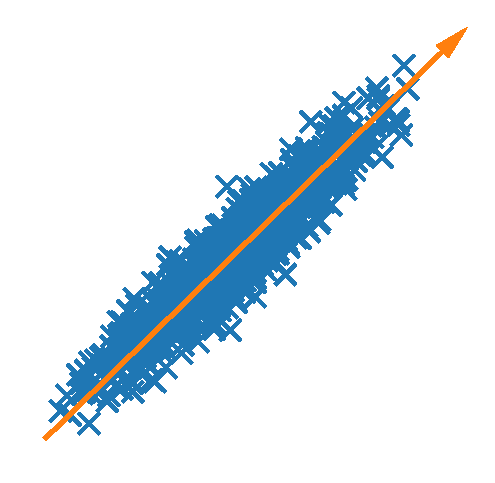
\includegraphics[width=0.3\textwidth]{figures/dimred/data_variance}
  \caption{La variance des donn�es en deux dimensions est maximale selon l'axe
    indiqu� par la fl�che.}
  \label{fig:data_variance}
\end{figure}


\subsection{Standardisation}
Dans la suite de cette section, nous supposons que les variables ont �t�
\textbf{standardis�es} de sorte � toutes avoir une moyenne de 0 et une variance
de 1, pour �viter que les variables qui prennent de grandes valeurs aient plus
d'importance que celles qui prennent de faibles valeurs. C'est un pr�-requis de
l'application de l'ACP.  Cette standardisation s'effectue par :
\begin{equation}
  \label{eq:standardization}
  x^i_j \leftarrow \frac{x^i_j - \overline{x_j}}{\sqrt{\frac1n 
      \sum_{l=1}^n (x^l_j - \overline{x_j})^2}},
\end{equation}
o� $\overline{x_j} = \frac1n \sum_{l=1}^n x^l_j.$ On dira alors que $X$ est
\textbf{centr�e} : chacune de ses colonnes a pour moyenne 0 et \textbf{r�duite} :
chacune de ses colonnes a pour variance 1.

\begin{exemple}
  Consid�rons la matrice de donn�es 
  \[
    X = \begin{bmatrix} 1.0 & 20.0 \\
      2.0 & 10.0 \\
      3.0 & 50.0 \\
      4.0 & 30.0 \\
      5.0 & 40.0 \\
    \end{bmatrix}.
  \]
  La variance de la premi�re colonne vaut $2.0$ tandis que celle de la deuxi�me
  colonne vaut $200.0$. Peut-on pour autant en conclure que la deuxi�me
  variable � varie � plus que la premi�re, alors que les valeurs qu'elle prend
  sont simplement proportionnelles � celles prises par la premi�re ?

  La version standardis�e de $X$ est
  \[
    \begin{bmatrix} -1.414 & -0.707 \\
      -0.707 & -1.414 \\
      0.0 & 1.414 \\
      0.707 & 0.0 \\
      1.414 & 0.707 
    \end{bmatrix}.
  \]
\end{exemple}


\subsection{D�composition spectrale de la covariance}
\paragraph{Proposition} 
Soit $X \in \RR^{n \times p}$ une matrice centr�e de covariance empirique
$\Sigma = \frac1n X^\top X$. Les composantes principales de $X$ sont les
vecteurs propres de $\Sigma$, ordonn�s par valeurs propres d�croissantes.

\paragraph{Preuve}
Consid�rons un vecteur $\ww \in \RR^p$. La projection de $X$ sur $\ww$ est
le vecteur $X \ww \in \RR^n$.
La moyenne de $X \ww$ vaut $0$ car les variables $(\xx_1, \dots, \xx_p)$ sont
elles-m�mes de moyenne nulle ($X$ �tant centr�e).
La variance de $X \ww$ vaut alors 
\begin{equation*}
  \text{Var}(X \ww) = \frac1n \sum_{i=1}^n \left( \sum_{j=1}^p x_j^i w_j \right)^2 = \ww^\top \Sigma \ww.
\end{equation*}    

Appelons maintenant $\ww_1 \in \RR^p$ la premi�re composante principale de $X$.
$\ww_1$ est de norme $1$ et tel que la variance de $X \ww_1$ est maximale :
\begin{equation}
  \label{eq:pc1}
  \ww_1 \in \argmax_{\ww \in \RR^p} \left( \ww^\top \Sigma \ww \right)  \text{\qquad avec } \ltwonorm{\ww_1}=1.
\end{equation}
Il s'agit d'un probl�me d'optimisation quadratique sous contrainte d'�galit�,
que l'on peut r�soudre (cf section 2.2.1 du poly d'Optimisation) en
introduisant le multiplicateur de Lagrange $\alpha_1 > 0$ et en �crivant le
lagrangien
\begin{equation*}
  L(\alpha_1, \ww) = \ww^\top \Sigma \ww - \alpha_1 
  \left( \ltwonorm{\ww} - 1 \right).
\end{equation*}
%Par dualit� forte, % $\min_{\ww \in \RR^p} w^\top \Sigma w = \max_{\alpha_1}
    % \inf_{\ww \in \RR^p} L(\alpha_1, \ww).$
Le maximum de $\ww^\top \Sigma \ww$ sous la contrainte $\ltwonorm{\ww_1}=1$ est
�gal � $\min_{\alpha_1} \sup_{\ww \in \RR^p} L(\alpha_1, \ww).$ Le supremum du
lagrangien est atteint en un point o� son gradient s'annule, c'est-�-dire qui
v�rifie
\begin{equation*}
  2 \Sigma \ww - 2 \alpha_1 \ww = 0.
\end{equation*}
Ainsi, $\Sigma \ww_1 = \alpha_1 \ww_1$ et $(\alpha_1, \ww_1)$ forment un couple
(valeur propre, vecteur propre) de $\Sigma$.

Parmi tous les vecteurs propres de $\Sigma$, $\ww_1$ est celui qui maximise la
variance $\ww_1^\top \Sigma \ww_1 = \alpha_1 \ltwonorm{\ww_1} = \alpha_1.$
Ainsi, $\alpha_1$ est la plus grande valeur propre de $\Sigma$ (rappelons que
$\Sigma$ �tant d�finie par $X^\top X$ est semi-d�finie positive et que toutes
ses valeurs propres sont positives.)

La deuxi�me composante principale de $X$ v�rifie
\begin{equation}
  \label{eq:pc2}
  \ww_2 = \argmax_{\ww \in \RR^p} \left( \ww^\top \Sigma \ww \right) \text{ \qquad; avec } \ltwonorm{\ww_2}=1
  \text{ et } \ww^\top\ww_1=0.
\end{equation}
Cette derni�re contrainte nous permet de garantir que la base des composantes
principales est orthonorm�e.

Nous introduisons donc maintenant deux multiplicateurs de Lagrange
$\alpha_2 > 0$ et $\beta_2 > 0$ et obtenons le lagrangien
\begin{equation*}
  L(\alpha_2, \beta_2, \ww) = \ww^\top \Sigma \ww - \alpha_2 
  \left(\ltwonorm{\ww}^2 - 1 \right)
  - \beta_2 \ww^\top\ww_1.
\end{equation*}
Comme pr�c�demment, son supremum en $\ww$ est atteint en un point o� son
gradient s'annule :
\begin{equation*}
  2 \Sigma \ww_2 - 2 \alpha_2 \ww_2 - \beta_2 \ww_1 = 0.
\end{equation*}
En multipliant � gauche par $\ww_1^\top$, on obtient
\begin{equation*}
  2 \ww_1^\top \Sigma \ww_2 - 2 \alpha_2 \ww_1^\top \ww_2 - 
  \beta_2 \ww_1^\top \ww_1 = 0
\end{equation*}
d'o� l'on conclut que $\beta_2=0$ et, en rempla�ant dans l'�quation pr�c�dente,
que, comme pour $\ww_1$, $2 \Sigma \ww_2 - 2 \alpha_1 \ww_2 = 0$.  Ainsi
$(\alpha_2, \ww_2)$ forment un couple (valeur propre, vecteur propre) de
$\Sigma$ et $\alpha_2$ est maximale : il s'agit donc n�cessairement de la
deuxi�me valeur propre de $\Sigma$.
    
Le raisonnement se poursuit de la m�me mani�re pour les composantes principales
suivantes. \hfill $\square$

  
\paragraph{Preuve alternative} Alternativement, on peut prouver ce th�or�me
en observant que $\Sigma$, �tant d�finie positive, est
diagonalisable par un changement de base orthonorm�e :
$\Sigma = Q^\top \Lambda Q$, o� $\Lambda \in \mathbb{R}^{p \times p}$ est une
matrice diagonale dont les valeurs diagonales sont les valeurs propres de
$\Sigma$.  Ainsi,
\begin{equation*}
  \ww_1^\top \Sigma \ww_1 = \ww_1^\top Q^\top \Lambda Q \ww_1 = 
  \left(Q \ww_1 \right)^\top \Lambda \left(Q \ww_1 \right).
\end{equation*}
Si l'on pose $\vv = Q \ww_1$, il s'agit donc pour maximiser
$\ww_1^\top \Sigma \ww_1$ de trouver $\vv$ de norme 1 ($Q$ �tant orthonorm�e et
$\ww_1$ de norme 1) qui maximise
\[\sum_{j=1}^p v_j^2 \lambda_j.\]  

Pour tout $j=1, \dots, p$, on a $\lambda_j \geq 0$ (car $\Sigma$ est d�finie
positive) et $0 \leq v_j^2 \leq 1$ car $\ltwonorm{\vv} = 1$. Ainsi, 
\[\sum_{j=1}^p v_j^2 \lambda_j \leq 
\left(\max_{j=1, \dots, p} \lambda_j \right)\sum_{j=1}^p
v_j^2 \leq \max_{j=1, \dots, p} \lambda_j,\]
et ce maximum est atteint quand $v_j=1$ et $v_k=0 \; \forall k \neq j$. On
retrouve ainsi que $\ww_1$ est le vecteur propre correspondant � la plus grande
valeur propre de $\Sigma$, et ainsi de suite. \hfill $\square$


\subsection{D�composition en valeurs singuli�res $\bigstar$}
\paragraph{Proposition} 
Soit $X \in \RR^{n \times p}$ une matrice centr�e. Les composantes principales
de $X$ sont ses vecteurs singuliers � droite ordonn�s par valeur singuli�re
d�croissante.

\paragraph{Preuve}
Factorisons $X$ sous la forme $U D V^\top$ avec $U \in \RR^{n \times n}$ et
$V \in \RR^{p \times p}$ orthogonales, et $D \in \RR^{n \times p}$ 
diagonale. Alors
\begin{equation*}
  \Sigma = X^\top X = V D U^\top U D V^\top = V D^2 V^\top
\end{equation*}
et les valeurs singuli�res de $X$ (les entr�es de $D$) sont les racines carr�es
des valeurs propres de $\Sigma$, tandis que les vecteurs singuliers � droite de
$X$ (les colonnes de $V$) sont les vecteurs propres de $\Sigma$. \hfill $\square$

  
En pratique, les impl�mentations de la d�composition en valeurs singuli�res (ou
SVD) sont num�riquement plus stables que celles de d�composition spectrale, et
c'est ainsi que l'ACP est impl�ment�e.

\subsection{Choix du nombre de composantes principales $\bigstar$}
R�duire la dimension des donn�es par une ACP implique de {\it choisir} un
nombre de composantes principales � conserver. Pour ce faire, on utilise la
\textbf{proportion de variance expliqu�e} par ces composantes : la variance de $X$
s'exprime comme la trace de $\Sigma$, qui est elle-m�me la somme de ses valeurs
propres.

Ainsi, si l'on d�cide de conserver les $m$ premi�res composantes principales de
$X$, la proportion de variance qu'elles expliquent est
\begin{equation*}
  \frac{\alpha_1 + \alpha_2 + \dots + \alpha_m}{\text{Tr}(\Sigma)}
\end{equation*}
o� $\alpha_1 \geq \alpha_2 \geq \dots \geq \alpha_p$ sont les valeurs propres
de $\Sigma$ par ordre d�croissant.
  
Il est classique de s'int�resser � l'�volution, avec le nombre de composantes,
soit de la proportion de variance expliqu�e par chacune d'entre elles, soit �
cette proportion cumul�e. On peut repr�senter visuellement ces proportions sur
un {\it scree plot} (figure~\ref{fig:scree_plots}), utilis� pour d�terminer le
nombre de composantes qui expliquent ensemble un pourcentage de la variance
fix� a priori ($95\%$ sur la figure~\ref{fig:scree_plot_cumul}), ou le nombre
de composantes � partir duquel ajouter une nouvelle composante n'est plus
informatif (� coude � sur la
figure~\ref{fig:scree_plot}). % Ce graphe peut nous servir
% � d�terminer visuellement soit le nombre de composantes principales qui
% expliquent un pourcentage de la variance que l'on s'est initialement fix�
% ($95\%$ sur la figure~\ref{fig:scree_plot}, soit le nombre de composantes
% principales correspondant au � coude � du scree plot cumulatif
% (figure~\ref{fig:scree_plot_cumul}), � partir duquel ajouter une nouvelle
% composante ne semble plus informatif.


\begin{figure}[h]
  \begin{subfigure}[t]{0.43\textwidth}
    \centering
    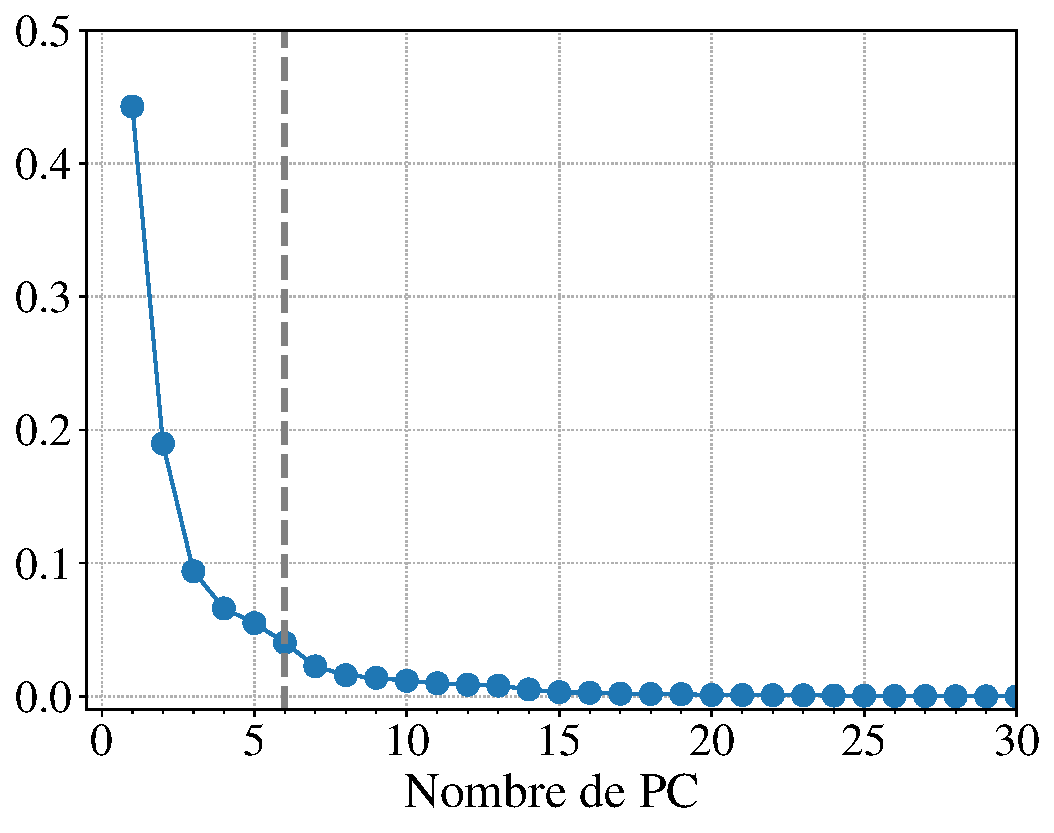
\includegraphics[width=\textwidth]{figures/dimred/scree_plot}
    \caption{Pourcentage de variance expliqu� par chacune des composantes
      principales. � partir de 6 composantes principales, ajouter de nouvelles
      composantes n'est plus vraiment informatif.}
    \label{fig:scree_plot}
  \end{subfigure} \hfill
  \begin{subfigure}[t]{0.43\textwidth}
    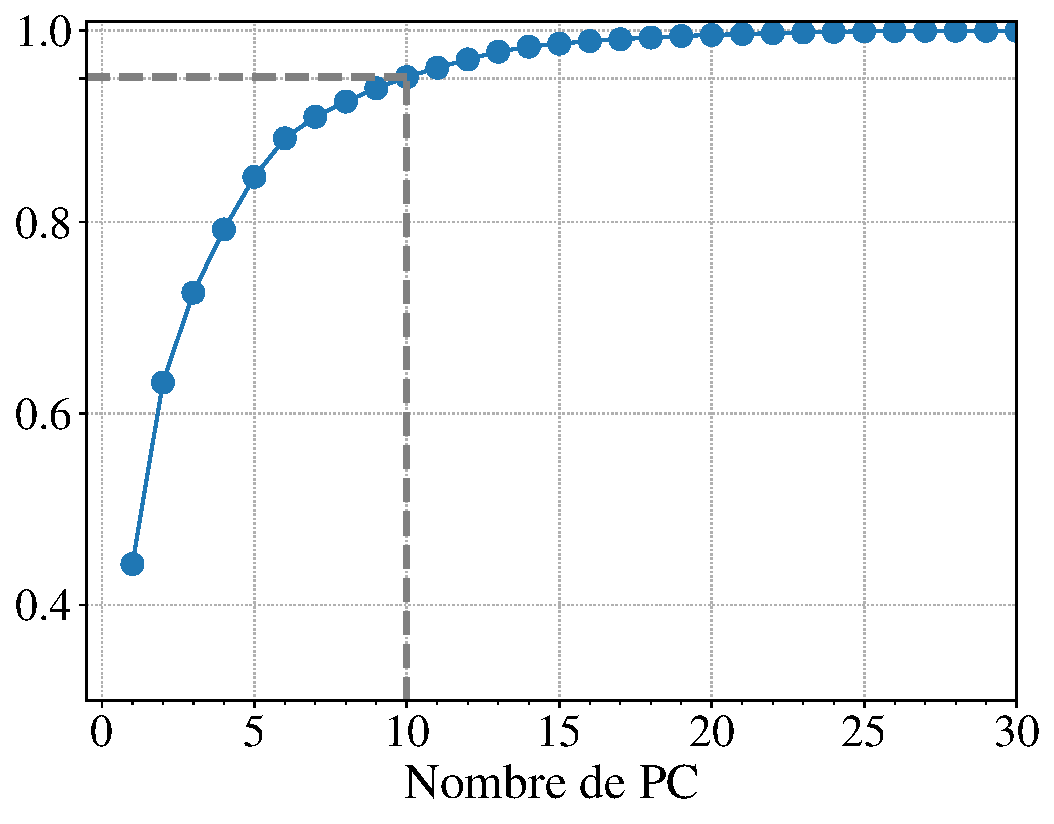
\includegraphics[width=\textwidth]{figures/dimred/scree_plot_cumul}  
    \caption{Pourcentage cumul� de variance expliqu�e par chacune des
      composantes principales. Si on se fixe une proportion de variance
      expliqu�e de $95\%$, on peut se contenter de 10 composantes principales.}
    \label{fig:scree_plot_cumul}
  \end{subfigure}
  \caption{Choix du nombre de PC � l'aide du
    pourcentage de variance expliqu�e.}
  \label{fig:scree_plots}
\end{figure}

\section{Factorisation de la matrice des donn�es $\bigstar$}
Soit un nombre $m$ de composantes principales, calcul�es par une ACP,
repr�sent�es par une matrice $W \in \RR^{p \times m}$. La repr�sentation
r�duite des $n$ observations dans le nouvel espace de dimension $m$ s'obtient
en projetant $X$ sur les colonnes de $W$, autrement dit en calculant
\begin{equation}
  \label{eq:reduced_rep}
  H = X W.
\end{equation}

La matrice $H \in \RR^{n \times m}$ peut �tre interpr�t�e comme une
\textbf{repr�sentation latente} (ou cach�e, {\it hidden} en anglais d'o� la
notation $H$) des donn�es. C'est cette repr�sentation que l'on a cherch� �
d�couvrir gr�ce � l'ACP.

Les colonnes de $W$ �tant des vecteurs orthonorm�s (il s'agit de vecteurs
propres de $X X^\top$), on peut multiplier l'�quation~\ref{eq:reduced_rep} �
droite par $W$ pour obtenir une {\it factorisation} de $X$ :
\begin{equation}
  \label{eq:pca_factor}
  X = H W^\top.
\end{equation}
Cette factorisation s'inscrit dans le cadre plus g�n�ral de \textbf{l'analyse
  factorielle}.

Elle correspond en effet � consid�rer que les donn�es sont les r�alisation d'un
vecteur al�atoire $(X_1, X_2, \dots, X_p)$ obtenues par
% \begin{equation}
%   \label{eq:fa_model}
%   (X_1, X_2, \dots, X_p)^\top = (H_1, H_2, \dots, H_m)^\top W + \epsilon,
% \end{equation}
\begin{equation}
  \label{eq:fa_model}
  (X_1, X_2, \dots, X_p) = W (H_1, H_2, \dots, H_m) + \epsilon,
\end{equation}
o� $(H_1, H_2, \dots, H_m)$ est le vecteur al�atoire latent qui g�n�re les
donn�es et $\epsilon$ un bruit gaussien : $\epsilon \sim \Ncal(0, \Psi),$ avec
$\Psi \in \RR^{p \times p}$.

Supposons maintenant que $(H_1, H_2, \dots, H_m)$ est un vecteur al�atoire
gaussien $m$-dimensionnel, d'esp�rance $0$ (les variables latentes sont elles
aussi centr�es) et de covariance $I_m$ o� $I_m$ est la matrice identit� de
dimensions $m \times m$. Alors $(X_1, X_2, \dots, X_p)$ est lui-m�me un vecteur
al�atoire gaussien, d'esp�rance nulle et de covariance $WW^\top + \Psi$.

Si l'on suppose de plus que $\epsilon$ est un bruit isotropique, autrement dit
que $\Psi = \sigma^2 I_p$, alors 
\[
  (X_1, X_2, \dots, X_p) \sim \Ncal (0, WW^\top + \sigma^2 I_p).
\] 
On peut alors estimer les param�tres $W$ et $\sigma^2$ par maximum de
vraisemblance ; c'est ce qu'on appelle l'\textbf{ACP probabiliste}.

L'ACP que nous venons de voir est un cas limite de l'ACP probabiliste, obtenu
quand la covariance du bruit devient infiniment petite
($\sigma^2 \rightarrow 0$)\footnote{Vous en trouverez la preuve dans l'article
  \textit{Probabilistic principal components analysis}, M.~E. Tipping \&
  C.~M. Bishop,  Journal of the Royal
    Statistical Society Series B, 61:611--622 (1999).}.

On peut plut�t faire la supposition plus g�n�rale que $\Psi$ est une matrice
diagonale. Les valeurs de $W$, $\Psi$ et $\sigma^2$ peuvent une fois de plus
�tre obtenues par maximum de vraisemblance. C'est ce que l'on appelle
\textbf{l'analyse factorielle}.  Dans l'analyse factorielle, les composantes
principales (les colonnes de $W$) ne sont pas n�cessairement orthogonales. En
particulier, il est donc possible d'obtenir des composantes d�g�n�r�es,
autrement dit des colonnes de $W$ dont toutes les coordonn�es sont $0$.

% \subsection{Approches non lin�aires}
% De nombreuses autres approches ont �t� propos�es pour r�duire la dimension des
% donn�es de mani�re non lin�aire. Parmi elles, nous en abordons ici
% quelques-unes parmi les plus populaires ; les expliquer de mani�re d�taill�e
% d�passe le propos de cet ouvrage introductif.

% \subsubsection{Analyse en composantes principales � noyau}
% Nous commencerons par noter que l'analyse en composantes principales se pr�te �
% l'utilisation de l'astuce du noyau (cf. section~\ref{sec:kernel_trick}). La
% m�thode qui en r�sulte est appel�e {\it kernel PCA}, ou {\it kPCA}.

% \subsubsection{Positionnement multidimensionnel}
% Le {\it positionnement multidimensionnel}, ou {\it multidimensional scaling}
% ({\it MDS})~\citep{cox1994}, se base sur une matrice de {\it dissimilarit�}
% $D \in \RR^{n \times n}$ entre les observations : il peut s'agir d'une distance
% m�trique, mais ce n'est pas n�cessaire. Le but de l'algorithme est alors de
% trouver une repr�sentation des donn�es qui pr�serve cette dissimilarit� :
% \begin{equation}
%   \label{eq:mds}
%   X^* = \argmin_{Z \in \RR^{n \times m}} \sum_{i=1}^n \sum_{l=i+1}^n \left( 
%     \ltwonorm{\zz^i - \zz^l} - D_{il}\right)^2.
% \end{equation}
% Si l'on utilise la distance euclidienne comme dissimilarit�, alors le MDS est
% �quivalent � une ACP.

% Le positionnement multidimensionnel peut aussi s'utiliser pour positionner dans
% un espace de dimension $m$ des points dont on ne conna�t pas les
% coordonn�es. Il s'applique par exemple tr�s bien � repositionner des villes sur
% une carte � partir uniquement des distances entre ces villes.

% Une des limitations de MDS est de ne chercher � conserver la distance entre les
% observations que globalement. Une fa�on efficace de construire la matrice de
% dissimilarit� de MDS de sorte � conserver la structure locale des donn�es est
% l'algorithme {\it IsoMap}~\citep{tenenbaum2000}. Il s'agit de construire un
% graphe de voisinage entre les observations en reliant chacune d'entre elles �
% ses $k$ plus proches observations voisines. Ces ar�tes peuvent �tre pond�r�e
% par la distance entre les observations qu'elles relient. Une dissimilarit�
% entre observations peut ensuite �tre calcul�e sur ce graphe de voisinage, par
% exemple via la longueur du plus court chemin entre deux points.

% \subsubsection{t-SNE}
% Enfin, l'algorithme {\it t-SNE}, pour {\it t-Student Neighborhood Embedding},
% propos� en 2008 par Laurens van der Maaten and Geoff Hinton, propose
% d'approcher la distribution des distances entre observations par une loi de
% Student~\citep{vandermaaten2008}. Pour chaque observation $\xx^i$, on d�finit
% $P_i$ comme la loi de probabilit� d�finie par
% \begin{equation}
%   P_i(\xx) = \frac1{\sqrt{2 \pi \sigma^2}} \exp \left( - \frac{
%       \ltwonorm{\xx - \xx^i}^2}{2 \sigma^2} \right).
%   \label{eq:tsne_distr}    
% \end{equation}
% t-SNE consiste alors � r�soudre
% \begin{equation}
%   \label{eq:tsne}
%   \argmin_{Q} \sum_{i=1}^n KL(P_i||Q_i)
% \end{equation}
% o� $KL$ d�note la divergence de Kullback-Leibler (voir
% section~\ref{sec:cross_entropy}) et $Q$ est choisie parmi les distributions de
% Student de dimension inf�rieure � $p$. Attention, cet algorithme trouve un
% minimum local et non global, et on pourra donc obtenir des r�sultats diff�rents
% en fonction de son initialisation. De plus, sa complexit� est quadratique en le
% nombre d'observations.
% \end{cours}

% \begin{pointsclefs}
% \item R�duire la dimension des donn�es avant d'utiliser un algorithme
%   d'apprentissage supervis� permet d'am�liorer ses besoins en temps et en
%   espace, mais aussi ses performances.
% \item On distingue la s�lection de variables, qui consiste � �liminer des
%   variables redondantes ou peu informatives, de l'extraction de variable, qui
%   consiste � g�n�rer une nouvelle repr�sentation des donn�es.
% \item Projeter les donn�es sur un espace de dimension 2 gr�ce �, par exemple,
%   une ACP ou t-SNE, permet de les visualiser.
% \item De nombreuses m�thodes permettent de r�duire la dimension des variables. 
% \end{pointsclefs}

% \section{Compl�ments}
% \subsection{Fl�au de la dimension}
% \label{sec:dimcurse}
% En haute dimension, les individus ont tendance � tous �tre �loign�s les uns des
% autres. Pour comprendre cette assertion, pla�ons-nous en dimension $p$ et
% consid�rons l'hypersph�re $\Scal(\xx, R)$ de rayon $R \in \RR_+^*$ centr�e sur
% une observation $\xx$, ainsi que l'hypercube $\Ccal(\xx, R)$ circonscrit �
% cette hypersph�re. Le volume de $\Scal(\xx)$ vaut
% $\frac{2 R^p \pi^{p/2}}{p \Gamma(p/2)}$, tandis que celui de $\Ccal(\xx, R)$,
% dont le c�t� a pour longueur $2R$, vaut $2^p R^p$. Ainsi
% \begin{equation*}
%   \lim_{p \rightarrow \infty} \frac{\text{Vol}(\Ccal(\xx, R))}{
%     \text{Vol}(\Scal(\xx, R))} = 0.
% \end{equation*}
% Cela signifie que la probabilit� qu'un exemple situ� dans $\Ccal(\xx, R)$
% appartienne � $\Scal(\xx, R)$, qui vaut $\frac{\pi}4 \approx 0.79$ lorsque
% $p=2$ et $\frac{\pi}6 \approx 0.52$ lorsque $p=3$, devient tr�s faible quand
% $p$ est grand : les donn�es ont tendance � �tre �loign�es les unes des autres.

% Cela implique que les algorithmes d�velopp�s en utilisant une notion de
% similarit� ou distance entre individus ne fonctionnent pas n�cessairement en
% grande dimension. Ainsi, r�duire la dimension peut �tre n�cessaire � la
% construction de bons mod�les d'apprentissage.


\begin{plusloin}
\item Une variante populaire de l'analyse factorielle est la
  \textbf{factorisation positive de matrice} (ou NMF pour \textit{non-negative
    matrix factorisation}), qui permet lorsque toutes les entr�es de $X$ sont
  positives, de chercher � la d�composer sous la forme $H W$ o� $H$ et $W$ ont
  elles aussi toutes leurs entr�es positives. Cela facilite leur
  interpr�tation.
\item Il existe de nombreuses approches de r�duction de dimension
  non-lin�aires, c'est-�-dire qui cr�ent des composantes qui ne sont pas des
  composantes lin�aires des variables initiales. Parmi elles, citons 
  \begin{itemize}
  \item le \textbf{positionnement multidimensionnel}, ou MDS pour {\it
      multidimensional scaling}, qui cherche � pr�server la distance entre les
    individus. Dans le cas de la distance euclidienne, on se ram�ne � l'ACP ;
    mais il est possible d'utiliser d'autres distances, y compris des distances
    non-m�triques.
  \item le \textbf{t-SNE} (prononc� � ti-sni �), pour {\it t-Student
      Neighborhood Embedding}, qui cherche � approcher la loi des distances
    entre individus par une loi de Student.
  \item le \textbf{UMAP}, pour {\it Uniform Manifold Approximation and
      Projection} qui suppose les individus uniform�ment distribu�s sur une
    vari�t� riemanienne qu'il s'agit d'approcher.
  \end{itemize}
\item Enfin, nous verrons au chapitre~\ref{chap:nonlin} que la derni�re couche
  cach�e d'un r�seau de neurones profond peut �tre consid�r�e comme une
  nouvelle repr�sentation des donn�es prises en entr�e par ce r�seau de
  neurones. On parle ainsi parfois d'apprentissage de repr�sentation
  (\textit{representation learning}) plut�t que d'apprentissage profond.
% \item Le tutoriel de \citet{shlens2014} est une introduction d�taill�e � l'analyse en
%   composantes principales.
% \item Pour une revue des m�thodes de s�lection de variables, on pourra se
%   r�ferer �~\citet{guyon2003}.
% \item Pour plus de d�tails sur la NMF, on pourra par exemple se tourner
%   vers~\citet{lee1999}
% \item Pour plus de d�tails sur les m�thodes des s�lection de sous-ensemble de
%   variables (wrapper methods), on pourra se r�f�rer �
%   l'ouvrage de~\citet{miller1990}
% \item Une page web est d�di�e � Isomap:
%   \url{http://web.mit.edu/cocosci/isomap/isomap.html}.
% \item Pour plus de d�tails sur l'utilisation de t-SNE, on pourra se r�f�rer �
%   la page \url{https://lvdmaaten.github.io/tsne/} ou � la publication
%   interactive de~\citet{wattenberg2016}.
\end{plusloin}

% \section*{Bibliographie}
% \vspace{-25pt}
% \begin{thebibliography}{99}
% \bibitem[\protect\astroncite{Cox et Cox}{1994}]{cox1994} Cox, T.~F. et Cox,
%   M. A.~A. (1994).  \newblock {\em Multidimensional Scaling}.  \newblock
%   Chapman and Hall., London.

% \bibitem[\protect\astroncite{Guyon et Elisseeff}{2003}]{guyon2003} Guyon,
%   I. et Elisseeff, A. (2003).  \newblock An introduction to variable and
%   feature selection.  \newblock {\em Journal of Machine Learning Research},
%   3:1157--1182.

% \bibitem[\protect\astroncite{Hinton}{2002}]{hinton2002} Hinton, G.~E. (2002).
%   \newblock Training product of experts by minimizing contrastive divergence.
%   \newblock {\em Neural Computation}, 14:1771--1800.

% \bibitem[\protect\astroncite{Hinton et Salakhutdinov}{2006}]{hinton2006}
%   Hinton, G.~E. et Salakhutdinov, R.~R. (2006).  \newblock Reducing the
%   dimensionality of data with neural networks.  \newblock {\em Science},
%   313:504--507.

% \bibitem[\protect\astroncite{Kozachenko et Leonenko}{1987}]{kozachenko1987}
%   Kozachenko, L.~F. et Leonenko, N.~N. (1987).  \newblock A statistical
%   estimate for the entropy of a random vector.  \newblock {\em Problemy
%     Peredachi Informatsii}, 23:9--16.

% \bibitem[\protect\astroncite{Lee et Seung}{1999}]{lee1999} Lee, D.~D. et
%   Seung, H.~S. (1999).  \newblock Learning the parts of objects by non-negative
%   matrix factorization.  \newblock {\em Nature}, 401(6755):788--791.

% \bibitem[\protect\astroncite{Miller}{1990}]{miller1990} Miller, A.~J. (1990).
%   \newblock {\em Subset Selection in Regression}.  \newblock Chapman and Hall.,
%   London.

% \bibitem[\protect\astroncite{Shlens}{2014}]{shlens2014} Shlens, J. (2014).
%   \newblock A {Tutorial} on {Principal} {Component} {Analysis}.  \newblock {\em
%     arXiv [cs, stat]}.  \newblock arXiv: 1404.1100.

% \bibitem[\protect\astroncite{Smolensky}{1986}]{smolensky1986} Smolensky,
%   P. (1986).  \newblock Information processing in dynamical systems:
%   foundations of harmony theory.  \newblock In {\em Parallel Distributed
%     Processing: Explorations in the Microstructure of Cognition}, volume 1:
%   Foundations, chapter~6, pages 194--281. MIT Press, Cambridge, MA.

% \bibitem[\protect\astroncite{Tenenbaum et~al.}{2000}]{tenenbaum2000} Tenenbaum,
%   J.~B., de~Silva, V., et Langford, J.~C. (2000).  \newblock A global
%   geometric framework for nonlinear dimensionality reduction.  \newblock {\em
%     Science}, 290(5500):2319--2323.

% \bibitem[\protect\astroncite{Tipping et Bishop}{1999}]{tipping1999} Tipping,
%   M.~E. et Bishop, C.~M. (1999).  \newblock Probabilistic principal components
%   analysis.  \newblock {\em Journal of the Royal Statistical Society Series B},
%   61:611--622.

% \bibitem[\protect\astroncite{van~der Maaten et Hinton}{2008}]{vandermaaten2008}
%   van~der Maaten, L. et Hinton, G. (2008).  \newblock Visualizing data using
%   t-{SNE}.  \newblock {\em Journal of Machine Learning Research}, 9:2579--2605.

% \bibitem[\protect\astroncite{Wattenberg et~al.}{2016}]{wattenberg2016}
%   Wattenberg, M., Vi�gas, F., et Johnson, I. (2016).  \newblock How to use
%   t-{SNE} effectively.  \newblock {\em Distill}.  \newblock
%   \url{http://distill.pub/2016/misread-tsne}.
% \end{thebibliography}



%%% Local Variables:
%%% mode: latex
%%% TeX-master: "sdd_2020_poly"
%%% End:

% \clearpage 

% \chapter{Bonnes pratiques}
% %-*- coding: iso-latin-1 -*-
\label{chap:pratiques}

\paragraph{Notions :} visualisation de donn�es, repr�sentativit� des donn�es,
�quit� des algorithmes, confidentialit� des donn�es, anonymisation,
responsabilit�.

\paragraph{Objectifs p�dagogiques :} 
\begin{itemize}      
  \setlength{\itemsep}{3pt}
\item S'interroger sur la pertinence d'une analyse de donn�es et la validit�
  des conclusions qui en sont tir�es.
\end{itemize}

La science des donn�es n'est pas uniquement une discipline technique : comme
souvent en ing�nierie, nous ne pouvons pas dissocier les calculs que nous
faisons de la question pos�e ni de leur utilisation. Ce chapitre n'a pas
vocation � �tre un cours d'�thique\footnote{L'�thique peut �tre
  d�finie comme l'�tude de la justification d'ue action � partir de normes,
  r�gles juridiques ou d�ontologiques, valeurs morales, intuitions et
  traditions qui peuvent �tre multiples et contradictoires au sein d'une m�me
  socit�t�.}, mais � vous donner quelques points d'entr�e pour vous amener �
vous poser des questions sur l'usage de la science des donn�es, de
l'apprentissage automaique et de l'intelligence artificielle. Pour cette
raison, vous trouverez plus de liens externes qu'� l'habitude � travers le
texte de ce chapitre, pointant tant vers des publications scientifiques que des
blogs de vulgarisation ou des articles de presse grand public. N'h�sitez pas �
poursuivre vos propres lectures sur le sujet.

Nous motiverons ce chapitre par deux citations : la premi�re, attribu�e �
Benjamin Disraeli par Mark Twain, ``\textit{There are three kinds of lies:
  lies, damned lies, and statistics}'', et la seconde, attribu�e � George
Box, ``\textit{All models are wrong, but some are useful}''.

\section{Visualisation de donn�es}
La fa�on dont vous choisissez de repr�senter vos donn�es ou vos r�sultats a un
impact fort sur le message que vous essayez de faire passer. 

Mi-mai 2020, le
Department of Public Health de l'�tat de G�orgie (�tats-Unis d'Am�rique) a
publi� le diagramme en barres de la figure~\ref{fig:georgia_wtf_barplot}. Regardez bien l'axe des abscisses : le message vous semble-t-il le m�me quand
les dates sont ordonn�es de mani�re chronologique, comme sur la figure~\ref{fig:georgia_fixed_barplot} ?

\begin{figure}[h]
  \centering
  \begin{subfigure}[t]{0.47\textwidth}
    \centering
    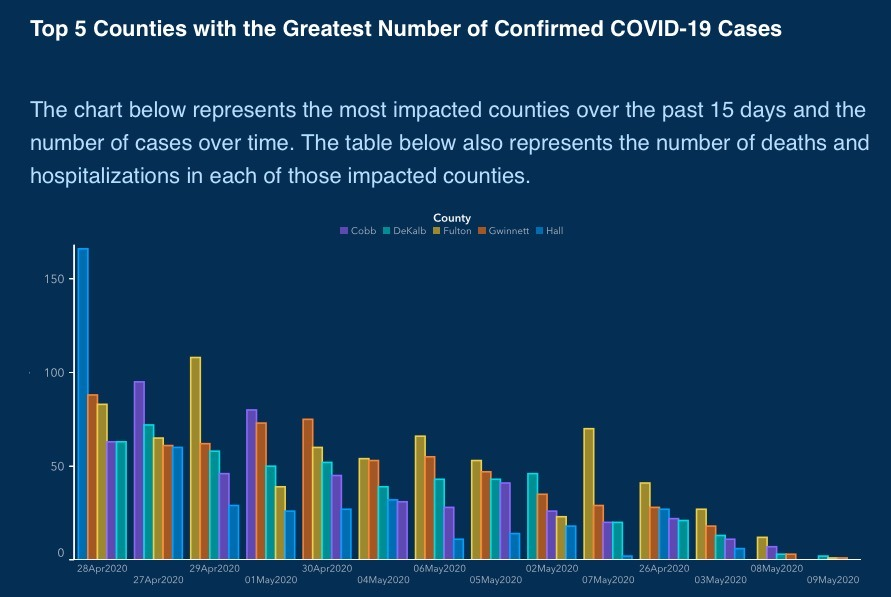
\includegraphics[width=\textwidth]{figures/pratiques/georgia_wtf_barplot}
    \caption{Premi�re version du diagramme en barres.}
    \label{fig:georgia_wtf_barplot}
  \end{subfigure} \hfill
  \begin{subfigure}[t]{0.47\textwidth}
    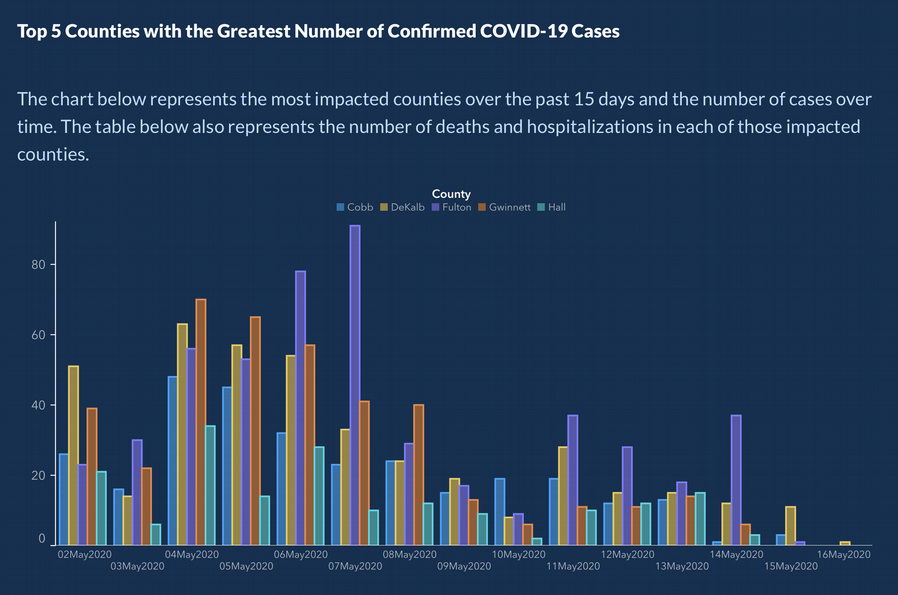
\includegraphics[width=\textwidth]{figures/pratiques/georgia_fixed_barplot}  
    \caption{Deuxi�me version du diagramme en barres.}
    \label{fig:georgia_fixed_barplot}
  \end{subfigure}  
  \caption{Deux variantes du m�me diagramme en barres publi�es par le
    Department of Public Health de l'�tat de G�orgie � propos du nombre de cas
    de CoVid19.}
  %\label{fig:georgia_barplot}
\end{figure}

Il est donc tr�s important de vous assurez que vos graphiques soient lisibles et qu'ils traduisent clairement votre message sans d�former les donn�es. La visualisation des donn�es, ou \textit{dataviz}, est un champ d'�tudes � part enti�re.  Nous nous contenterons ici de citer quelques principes parmi
les plus importants.


\subsection{Le choix des axes}
%https://callingbullshit.org/tools/tools_misleading_axes.html 
Le choix des �chelles et intervalles d'un graphique a une influence sur son
interpr�tation.

Pour un diagramme en barres, ne pas faire commencer les axes � 0 peut
artificiellement gonfler les diff�rences entre les diff�rentes barres. Ainsi,
le diagramme de la figure~\ref{fig:bars_start_nonzero} indique que le mod�le 4
est bien sup�rieur aux autres, tandis que celui de la
figure~\ref{fig:bars_start_zero} montre des performances tr�s comparables entre
les diff�rentes m�thodes. (Dans ce cas pr�cis, il serait de toute fa�on
souhaitable de r�p�ter plusieurs fois l'entrainement et l'�valuation, par
exemple avec une validation crois�e (que nous verrons
section~\ref{sec:crossval}) et de produire des barres d'erreurs.)
\begin{figure}[h]
  \centering
  \begin{subfigure}[t]{0.47\textwidth}
    \centering
    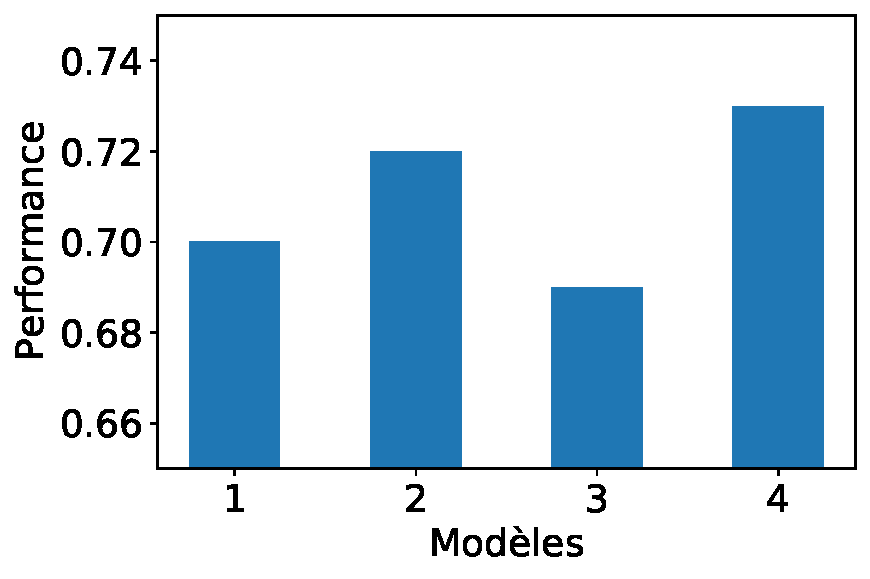
\includegraphics[width=\textwidth]{figures/pratiques/bars_start_nonzero}
    \caption{Axe des ordonn�es r�duit.}
    \label{fig:bars_start_nonzero}
  \end{subfigure} \hfill
  \begin{subfigure}[t]{0.47\textwidth}
    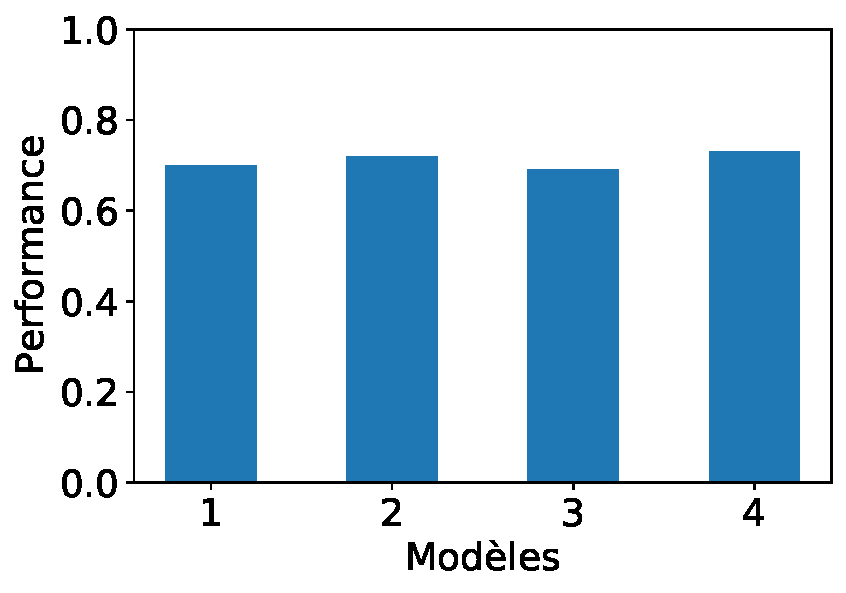
\includegraphics[width=\textwidth]{figures/pratiques/bars_start_zero}  
    \caption{Axe des ordonn�es allant de 0 � 1.}
    \label{fig:bars_start_zero}
  \end{subfigure}  
  \caption{Deux fa�ons de pr�senter la comparaison des performances de 4 mod�les.}
  %\label{fig:georgia_barplot}
\end{figure}

� l'inverse, il pourra �tre pr�f�rable pour un diagramme dont le but est non
pas de comparer les valeurs absolues de variables mais plut�t de pr�senter leur
�volution que l'axe des ordonn�es ne commence pas � z�ro. Ainsi, la figure~\ref{fig:line_start_zero} indique une temp�rature tr�s stable, tandis que la figure~\ref{fig:line_start_nonzero} permet de mieux rendre compte des variations.
\begin{figure}[h]
  \centering
  \begin{subfigure}[t]{0.47\textwidth}
    \centering
    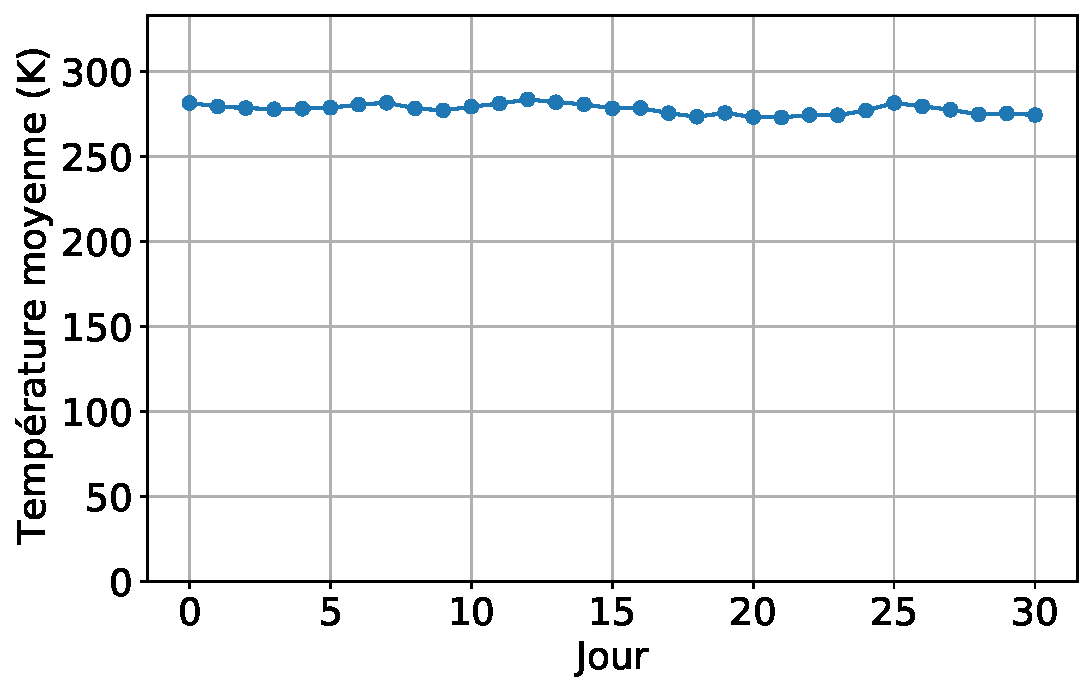
\includegraphics[width=\textwidth]{figures/pratiques/line_start_zero}
    \caption{Axe des ordonn�es partant de 0K.}
    \label{fig:line_start_zero}
  \end{subfigure} \hfill
  \begin{subfigure}[t]{0.47\textwidth}
    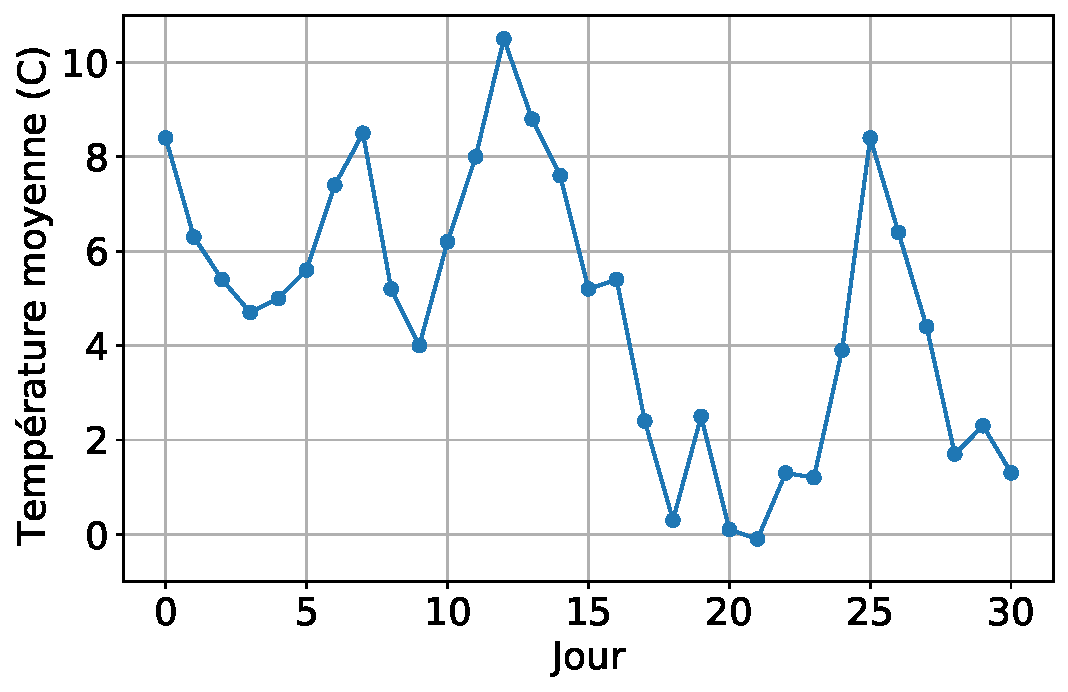
\includegraphics[width=\textwidth]{figures/pratiques/line_start_nonzero}  
    \caption{Axe des ordonn�es r�duit.}
    \label{fig:line_start_nonzero}
  \end{subfigure}  
  \caption{Deux fa�ons de pr�senter l'�volution des temp�ratures moyenne de la table~\ref{tab:meteo_data}.}
  %\label{fig:georgia_barplot}
\end{figure}

\subsection{\textit{Proportional ink} ou principe de l'encre proportionnelle}
%https://callingbullshit.org/tools/tools_proportional_ink.html
De mani�re g�n�rale, il est recommand�, lorsque l'on utilise des surfaces pour
repr�senter des nombres (par exemple, les rectangles d'un diagramme en barres),
que ces surfaces soient d'aires proportionnelles aux nombres en question. On
retrouve d'ailleurs ici l'id�e de commencer les barres d'un diagramme en
barres � 0.

Il faut cependant faire aussi attention � ce que les surfaces en question soient faciles � comparer visuellement. Un diagramme camembert est ainsi pr�f�rable � un graphique � bulles ; mais un diagramme en barres est g�n�ralement plus lisible qu'un diagramme camembert. La figure~\ref{fig:areas} l'illustre. Il s'agit d'une variante d'une \href{https://www.jstor.org/stable/2288400?seq=1#metadata\_info\_tab\_contents}{exp�rience men�e au d�but des ann�es 1980} et souvent consid�r�e comme fondatrice en \textit{dataviz}.

Remarquez ici que le diagramme en barres serait encore plus lisible sans couleurs (elles n'apportent rien) et en ordonnant les cat�gories par proportion.
\begin{figure}[h]
  \centering
  \begin{subfigure}[t]{0.20\textwidth}
    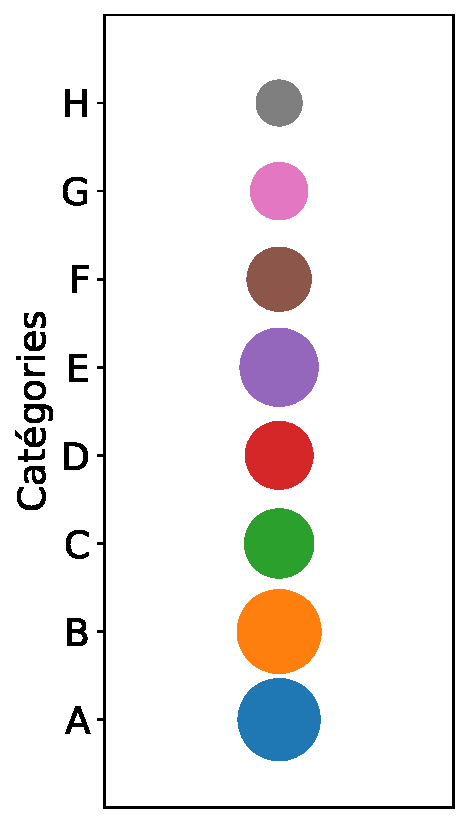
\includegraphics[width=\textwidth]{figures/pratiques/areas_bubbles}  
    \caption{Graphique � bulles.}
    \label{fig:areas_bubbles}
  \end{subfigure}  \hfill
  \begin{subfigure}[t]{0.33\textwidth}
    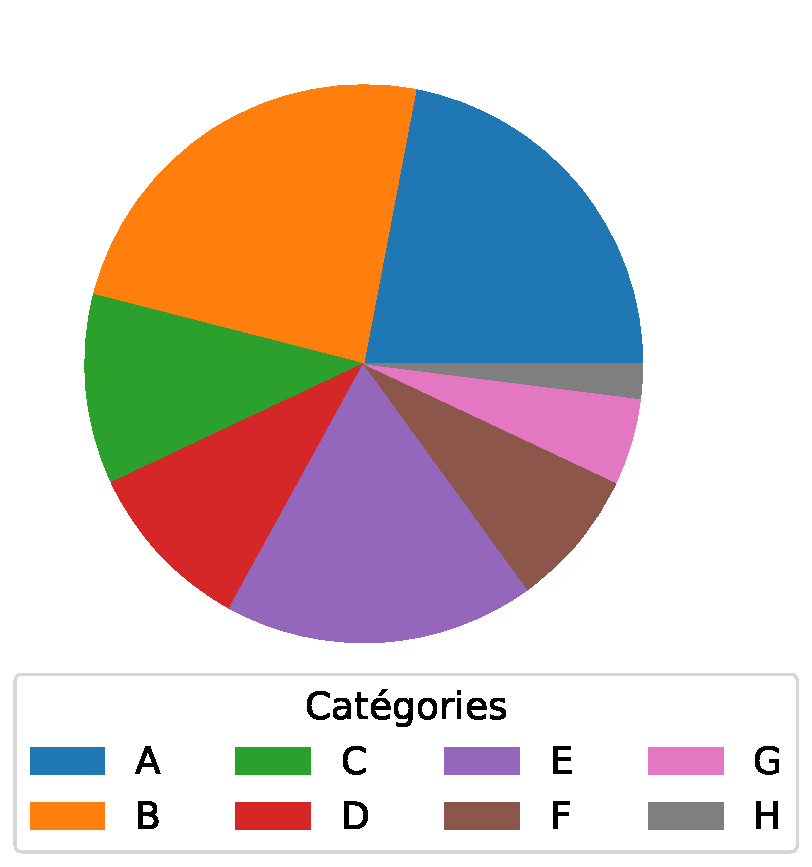
\includegraphics[width=\textwidth]{figures/pratiques/areas_pie}  
    \caption{Diagramme camembert.}
    \label{fig:areas_pie}
  \end{subfigure} \hfill
  \begin{subfigure}[t]{0.33\textwidth}
    \centering
    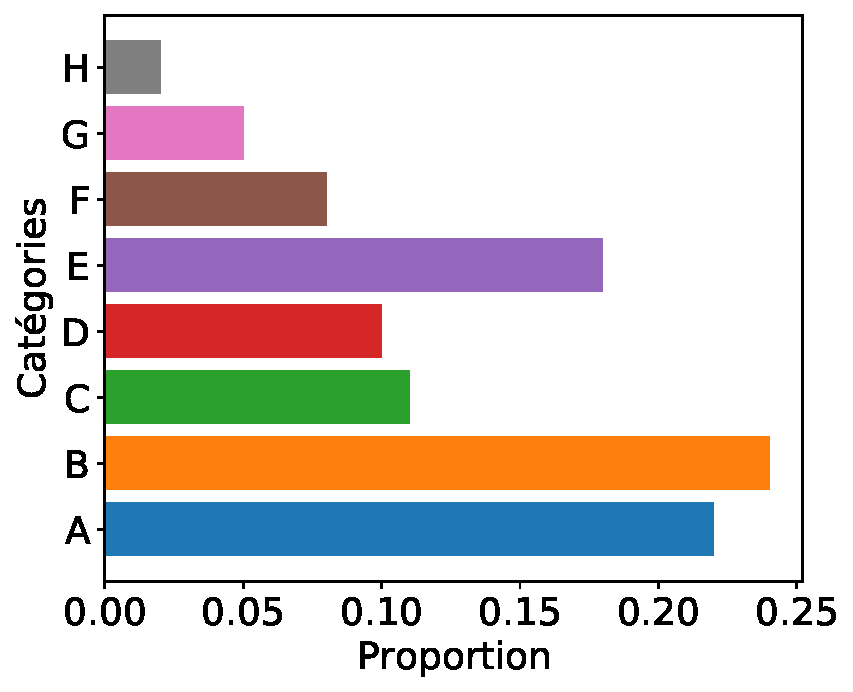
\includegraphics[width=\textwidth]{figures/pratiques/areas_bars}
    \caption{Diagramme en barres.}
    \label{fig:areas_bars}
  \end{subfigure} 
  \caption{Trois fa�ons de repr�senter les proportions de 8 cat�gories. Quelle(s) repr�sentation(s) permettent de les classer ais�ment par ordre croissant ?}
  \label{fig:areas}
\end{figure}

%\subsection{Attention aux r�sum�s}
%https://python-graph-gallery.com/39-hidden-data-under-boxplot/ 


\subsection{Dyschromatopie}
Nous ne percevons pas les couleurs de la m�me fa�on. Une forte proportion de la population est atteinte d'une forme ou d'une autre de dyschromatopie, la plus fr�quente �tant la deut�ranopie (incapacit� de diff�rencier rouge et vert). 

Pour assurer une accessibilit� maximale, utilisez des �chelles de couleurs adapt�es. Il est difficile de s'adapter � \textit{toutes} les dyschromatopies ; n�anmoins le cycle par d�faut de \texttt{matplotlib} est suppos� �tre relativement adapt�. Pour des \textit{heatmaps}, favoriser les �chelles de couleur \textit{viridis} ou \textit{cividis} (voir figure~\ref{fig:pca_plot}). Des outils comme \href{https://www.color-blindness.com/coblis-color-blindness-simulator/}{CBLIS} ou \href{https://www.funkify.org}{Funkify} vous permettent de simuler diff�rentes dyschromatopies pour v�rifier la lisibilit� de vos graphiques.


Vous pouvez aussi augmenter la lisibilit� de vos graphiques en utilisant des
indices suppl�mentaires (�paisseur de trait, hachures, forme des points,
ordonner les l�gendes dans le m�me ordre que les courbes, etc.) et en doublant
vos images d'une description textuelle alternative pour les personnes
non-voyantes.


\begin{figure}[h]
  \centering
  \begin{subfigure}[t]{0.30\textwidth}
    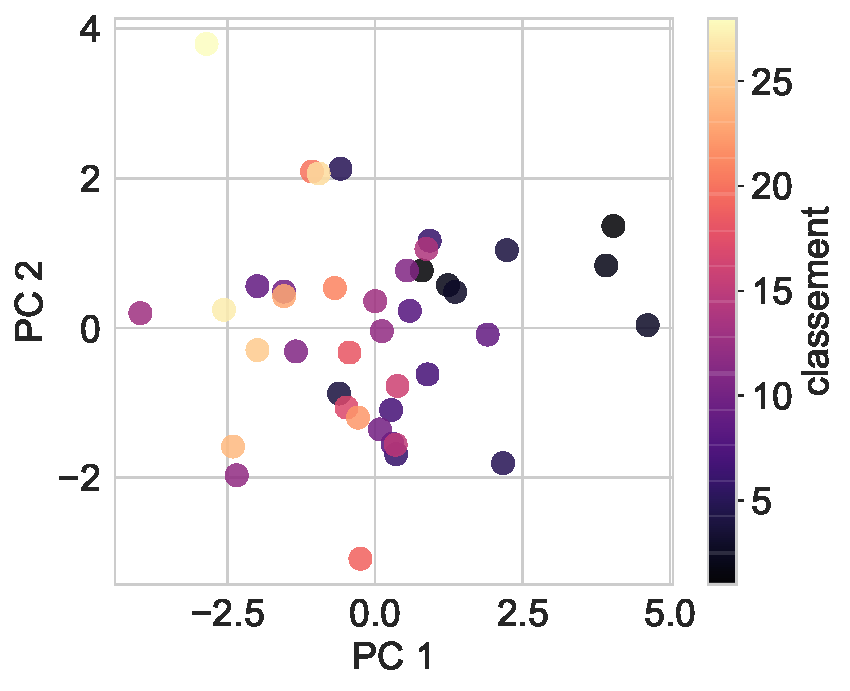
\includegraphics[width=\textwidth]{figures/pratiques/pca_plot_magma}  
    \caption{Magma.}
    \label{fig:pca_plot_magma}
  \end{subfigure}  \hfill
  \begin{subfigure}[t]{0.30\textwidth}
    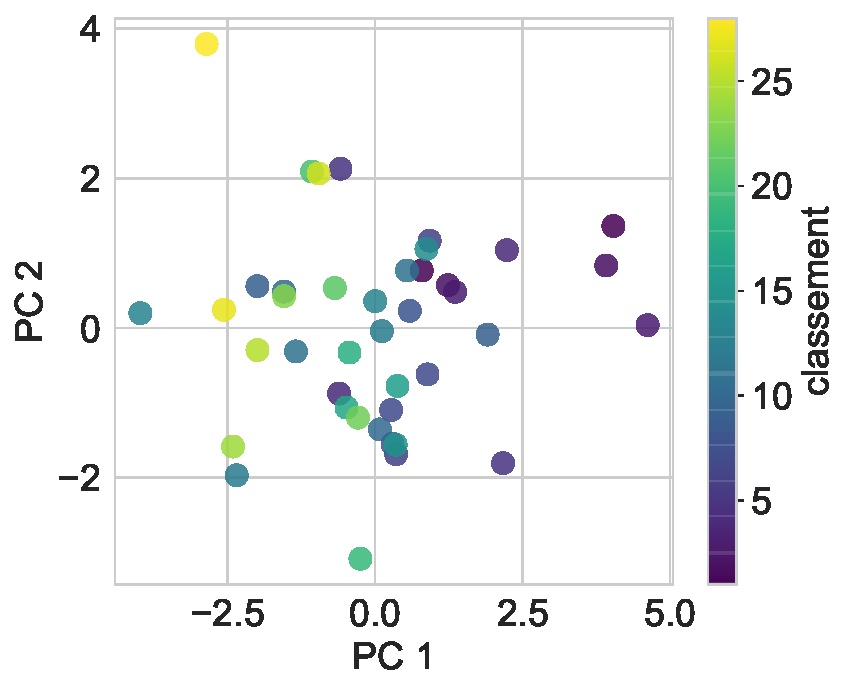
\includegraphics[width=\textwidth]{figures/pratiques/pca_plot_viridis}  
    \caption{Viridis.}
    \label{fig:pca_plot_viridis}
  \end{subfigure} \hfill
  \begin{subfigure}[t]{0.30\textwidth}
    \centering
    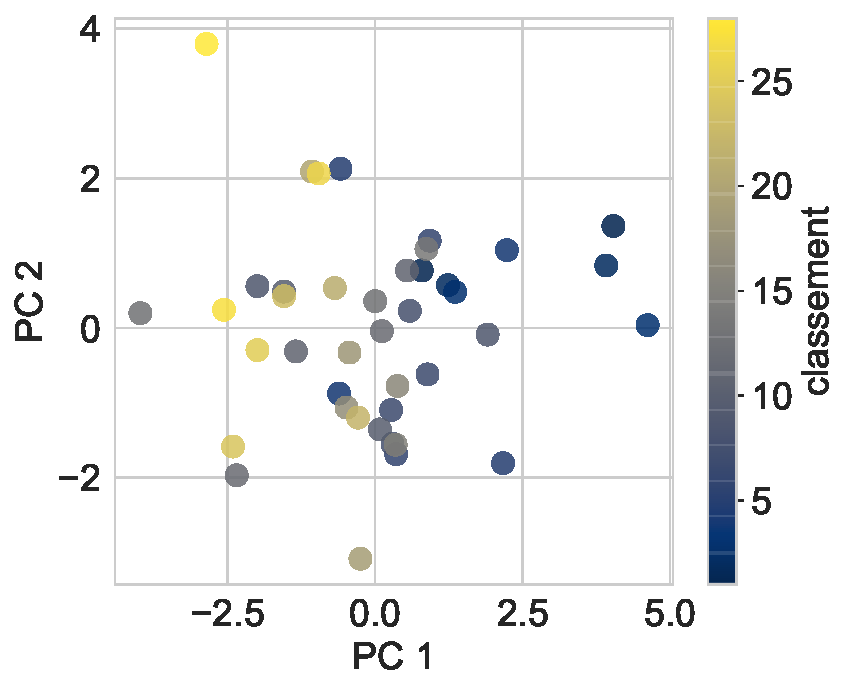
\includegraphics[width=\textwidth]{figures/pratiques/pca_plot_cividis}
    \caption{Cividis.}
    \label{fig:pca_plot_cividis}
  \end{subfigure} 
  \caption{Athl�tes de la PC2, repr�sent�s selon deux composantes, et color�s en fonction de leur classement, selon trois �chelles de couleur diff�rentes.}
  \label{fig:pca_plot}
\end{figure}




\section{�quit� des algorithmes}
Une question importante qui se pose constamment en science des donn�es est
celle de la \textbf{reproduction des biais}. En effet, un mod�le appris sur un
jeu de donn�es peut facilement reproduire des biais de ce jeu de donn�es,
qu'ils soient explicites ou implicites.

Un exemple qui revient souvent est celui d'un algorithme de ressources humaines
utilis� par Amazon. Le mod�le avait tendance � rejeter les candidatures pos�es
par des femmes. En effet, il �tait entra�n� sur des donn�es internes �
l'entreprise, dont les recrutements �taient fortement biais�s en faveur des
hommes. Bien que le genre n'ait pas �t� une variable utilis�e pour d�crire les
candidatures, le mod�le d�tectait dans le texte des CV des informations
corr�l�e dans le jeu d'entra�nement au rejet d'une candidature mais qui
s'av�raient surtout traduire qu'elle �tait pos�e par une femme (�ducation dans
un �tablissement non-mixte r�serv� aux femmes ; appartenance � une �quipe de
sport f�minin, etc.).

Ainsi, ce n'est pas parce qu'un mod�le statistique est purement math�matique
qu'il est impartial ; en particulier, un mod�le ne peut pas �tre de meilleure
qualit� que son jeu d'entra�nement. Il faut donc r�fl�chir � la
\textbf{repr�sentativit�} des donn�es : peut-on bien consid�rer qu'il s'agit
d'un �chantillon al�atoire de la population qui nous int�resse, o� ne
correspondent-elles qu'� une sous-population sp�cifique ?

Un autre exemple de reproduction des biais apparait dans une publication de
2016 qui pr�sente un classifieur capable de distinguer criminels de
non-criminels � partir de simples photos. Cependant, les clich�s de criminels
�taient des photos administratives prises de face, sans sourire, tandis que les
photos de non-criminels �taient des clich�s plus flatteurs : le mod�le
\href{https://callingbullshit.org/case\_studies/case\_study\_criminal\_machine\_learning.html}{d�tectait
  en fait les sourires}. On retrouve tr�s souvent ce type d'erreurs, d�es � un
\textbf{facteur confondant} : on croit arriver � s�parer des images sur leur
contenu alors qu'on utilise principalement leur luminosit� ; ou � trouver des
facteurs g�n�tiques influen�ant le niveau �conomique, alors que celui-ci est
fortement corr�l� dans les donn�es � la couleur de peau ; et ainsi de suite.

La question de l'�quit� des algorithmes est un sous-domaine important de
l'apprentissage automatique, et se pose d'autant plus que ses applications
s'�tendent � des domaines divers et vari�s touchant de nombreux aspects de nos
soci�t�s : recrutement mais aussi s�curit�, sant�, justice, etc. 
C'est le sujet par exemple de l'organisation
\href{https://www.fatml.org/}{Fairness, Accountability and Transparency in
  Machine Learning}.

Pour autant, il n'y a pas actuellement (et il n'y aura vraisemblablement
jamais) d'outils ou de proc�dures permettant de garantir cette �quit�. Il est
ainsi n�cessaire de comprendre l'origine possible des biais, ainsi que de
d�velopper des outils pour les mesurer.

Ces derni�res ann�es ont cependant vu l'�mergence de labels, tels que le
\href{http://fdu-label.com/fr/index.html}{Fair Data Use} en France ou
\href{http://aequitas.dssg.io/}{Aequitas} aux USA, proposant une �valuation
�thique des outils num�riques.

\section{Fiabilit�}
Du diagnostic automatis� aux v�hicules autonomes, nous avons de plus en plus
envie de faire confiance � l'intelligence artificielle pour les opportunit�s
qu'elle pr�sente.

Mais comment faire confiance aux mod�les et algorithmes issus de la science des
donn�es ? Plusieurs questions se posent en plus de celle de l'�quit� discut�e plus haut.

\paragraph{V�rifiabilit�} les syst�mes d'IA ont-ils le comportement attendu ?
Les \href{https://fr.wikipedia.org/wiki/M\%C3\%A9thode\_formelle\_(informatique)}{m�thodes
  formelles}
typiquement utilis�es en informatique pour les programmes utilis�s en avionique
ne se pr�tent gu�re aux mod�les de l'apprentissage automatique, m�me si \href{https://formal-paris-saclay.fr/}{de
r�cents travaux �mergent sur le sujet}.

\paragraph{Explicabilit� et interpr�tabilit�} Il s'agit aussi de vastes champs
d'�tude. Si une r�gression lin�aire est relativement interpr�table (cf. PC 3),
des mod�les param�triques plus complexes tels que ceux produits par des r�seaux
de neurones artificiels (voir chapitre~\ref{chap:nonlin}) le
sont beaucoup moins. 

\paragraph{Sp�cification} La description pr�cise du comportement attendu
peut-elle aussi �tre d�licate : quel choix doit faire un v�hicule autonome
entre renverser une fillette et emboutir une moto avec deux passagers ? Le MIT
Media Lab propose par exemple \href{http://moralmachine.mit.edu/hl/fr}{La
  Machine Morale}, une plateforme permettant d'explorer divers dilemnes moraux
pos�s par la prise de d�cision de machines intelligentes.

\paragraph{Robustesse} Les mod�les sont-ils robustes aux attaques ? Depuis
2015, les exemples montrant qu'il est possible d'induire facilement en erreur
un mod�le appris par apprentissage automatique s'accumulent. Ces exemples
incluent l'ajout de bruit
\footnote{https://arxiv.org/abs/1412.6572}{ind�tectable � l'\oe{}il} ou
\href{https://nicholas.carlini.com/code/audio\_adversarial\_examples}{�
  l'oreille}, la \href{https://arxiv.org/abs/1710.08864}{modification d'un seul
  pixel} d'une image, ou
l'\href{https://towardsdatascience.com/poisoning-attacks-on-machine-learning-1ff247c254db}{empoisonnement}
d'un jeu de donn�es, qui consiste � introduire au moment de l'apprentissage un
faible nombre d'exemples mal �tiquet�s ou ing�nieusement calibr�s pour induire
un comportement ind�sirable.

De m�me qu'en cryptographie o� de nouveaux protocoles �mergent pour faire face
� de nouvelles attaques de hackers, l'apprentissage automatique progresse aussi
pour r�pondre aux attaques
adversariales. \href{http://proceedings.mlr.press/v97/simon-gabriel19a.html}{De
  r�cents travaux} montrent m�me qu'en raison du fl�au de la dimension, les
attaques adversariales sont in�vitables en grande dimension.

\paragraph{Reproductibilit�} La d�marche scientifique repose sur la
reproductibilit� des exp�riences. Au probl�me du \textit{p-hacking} abord� au
Chapitre~\ref{chap:tests} s'ajoute celui de la disponibilit� des donn�es, qui
peut �tre limit�e pour des raisons de confidentialit�, ainsi que la question
des \textbf{ressources informatiques} qui peuvent �tre n�cessaires � entra�ner
certains mod�les. Reproduire des r�sultats obtenuse en faisant tourner 800
processeurs graphiques (GPUs) pendant 3 semaines n�cessite des ressources
financi�res importantes (on rejoint ici des questions de co�t �nerg�tique et
�cologique abord�es dans la section~\ref{sec:ecology}).


\paragraph{Responsabilit�} Qui est responsable en cas de faillite d'un
syst�me d'IA : l'IA est-elle responsable ? Ou bien la personne qui l'utilise ?
Ou encore celle qui l'a construite ? La question s'est par exemple pos�e
lorsqu'un v�hicule autonome
\href{https://www.nextinpact.com/news/108432-cause-probable-accident-mortel-uber-tout-monde-en-prend-pour-son-grade.htm}{a
  fauch� une pi�tonne} en mars 2018.



\section{Confidentialit� des donn�es}
Une grande partie des donn�es utilis�es en science des donn�es sont des donn�es
personnelles, c'est-�-dire que les individus qu'elles d�crivent sont des
personnes. Nombre d'entre nous s'inqui�tent de ce que les donn�es qui nous
concernent, qu'elles soient m�dicales, de localisation g�ographique, ou
concernent notre activit� num�rique, soient utilis�es � bon escient.

Les \href{https://risques-tracage.fr/}{discussions autour des applications de
  tra�age de contacts} dans la lutte contre la propagation du coronavirus vont
actuellement bon train, illustrant cette pr�occupation.


En tant que \textit{data scientists}, comment nous assurer que nous ne
compromettons pas la confidentialit� des personnes dont nous manipulons les
donn�es ? Deux types de solutions techniques sont possibles.
\paragraph{D�-identification algorithmique} Il s'agit de s'assurer que l'on ne
puisse pas remonter des donn�es aux individus. Parmi ces techniques,
l'\textbf{anonymisation} consiste � supprimer suffisamment d'informations
identifiantes pour emp�cher la r�identification. Ces informations peuvent �tre
\textbf{directement identifiantes} s'il s'agit de caract�ristiques personnelles
uniques (nom, num�ro de s�curit� sociale, num�ro de t�l�phone, etc.) ou
\textbf{indirectement identifiantes} si elles permettent d'identifier la
personne de mani�re unique quand elles sont crois�es avec d'autres donn�es (code postal, date de naissance et lieu de travail pris ensemble
peuvent �tre indirectement identifiants).  Par contraste, la
\textbf{confidentialit� diff�rentielle}, ou \textit{differential privacy} en
anglais cherche plut�t � garantir que les r�sultats d'une analyse sur une base de
donn�es soient presque identiques qu'un �chantillon soit pr�sent ou non.

\paragraph{S�curit� des bases de donn�es} Cet aspect inclut par exemple le
chiffrement homomorphique permettant d'obtenir les m�mes r�sultats sur donn�es
chiffr�es que non chiffr�es, ne laissant ainsi aux \textit{data scientists} que
l'acc�s aux donn�es chiffr�es, des solutions de calcul distribu� s�curis�es, ou
encore du mat�riel cryptographique permettant d'ex�cuter du code sans que les
donn�es ne soient visibles.

En France, la \href{https://www.cnil.fr/}{Commission Nationale de
  l'Informatique et des Libert�s (CNIL)} encadre l'utilisation des donn�es
personnelles, qui est notamment encadr� par la loi du 14 mai 2018 transposant
le
\href{https://fr.wikipedia.org/wiki/R\%C3\%A8glement\_g\%C3\%A9n\%C3\%A9ral\_sur\_la\_protection\_des\_donn\%C3\%A9es}{R�glement
  G�n�ral sur la Protection des Donn�es (RGPD)} de l'Union Europ�enne.


\section{Enjeux �cologiques}
\label{sec:ecology}
\href{https://www.ademe.fr/sites/default/files/assets/documents/guide-pratique-face-cachee-numerique.pdf}{Selon
  l'ADEME}, le secteur du num�rique est responsable de 4\% des �missions
mondiales de gaz � effet de serre, dont un quart d�s aux data
centers. Entra�ner un r�seau de neurones artificiels avec 213 millions de
param�tres peut g�n�rer \href{https://arxiv.org/abs/1906.02243}{autant
  d'�missions de CO2 que cinq voitures am�ricaines} pendant toute leur
existence, fabrication comprise.  Le
\href{https://mlco2.github.io/impact/}{Machine Learning Emissions Calculator}
est un des outils qui accompagnent la prise de conscience de l'impact
environnemental de la science des donn�es.


\begin{plusloin}
\item Des ouvrages entiers ont �t�s �crits sur la \textit{dataviz}, par exemple \href{https://serialmentor.com/dataviz/}{\textit{Fundamentals of Data Vizualization} de Claus O. Wilke}, le travail d'\href{https://www.edwardtufte.com/tufte/}{Edward Tufte}, ou encore \href{https://informationisbeautiful.net/}{\textit{Information is Beautiful} by David McCandless}.
\item \href{https://hippocrate.tech/}{Le Serment d'Hippocrate pour Data Scientist} de Data for Good.
\item La question de la repr�sentativit� se pose dans de nombreux
  domaines de l'ing�nierie. Les exemples sont nombreux, des
  \href{https://www.huffingtonpost.fr/2017/08/19/ce-distributeur-automatique-ne-distribue-pas-de-savon-aux-mains\_a\_23152387/}{distributeurs
    de savon qui ne d�tectent que les peaux claires} � tous les
  objets plut�t adapt�s aux hommes recens�s par Caroline Criado
  Perez dans
  \href{https://www.liberation.fr/france/2020/03/06/les-femmes-invisibles-dans-un-monde-cree-pour-les-hommes\_1780895}{\textit{Invisible
      Women}}.
  \item Un �pisode de La M�thode Scientifique  intitul� \href{https://april.org/ethique-numerique-des-datas-sous-serment-emission-la-methode-scientifique}{\textit{�thique num�rique, des data sous
    serment}}.
  \item {Fairness and Machine Learning} by Solon
    Barocas, Moritz Hardt and Arvind Narayanan.
  \item � propos de \href{https://www.latribune.fr/supplement/ceux-qui-transforment-la-france/la-justice-predictive-nouvel-outil-pour-les-professionnels-du-droit-837752.html}{justice pr�dictive}, l'article \href{https://www.dalloz-actualite.fr/flash/justice-et-intelligence-artificielle-preparer-demain-episode-i#.XsvEykNS8Xc}{Justice
        et intelligence artificielle : pr�parer demain}.
  \item \href{https://hbr.org/2013/04/the-hidden-biases-in-big-data}{\textit{The Hidden Biases in Big Data}}, Kate Crawford, HBR, April 2013. 
  \item \href{https://salil.seas.harvard.edu/files/salil/files/differential_privacy_primer_nontechnical_audience.pdf}{\textit{Differential privacy: A primer for a non-technical audience}}, A. Wood et al., Vanderbilt Journal of Entertainment and Technology Law.
\end{plusloin}

%%% Local Variables:
%%% mode: latex
%%% TeX-master: "sdd_2020_poly"
%%% End:



% \part{Apprentissage supervis�}
% \chapter{Minimisation du risque empirique}
% %-*- coding: iso-latin-1 -*-
\label{chap:erm}

\todo{
  \begin{itemize}
  \item Coh�rence des notations avec les chapitres pr�c�dents.
  \item Lien avec le cours d'optimisation.
  \item All�ger / �laguer.
  \end{itemize}
}

\paragraph{Notions :} classification, r�gression, espace des hypoth�ses,
minimisation du risque empirique, moindres carr�s, mod�les param�triques
lin�aires
\paragraph{Objectifs p�dagogiques :} 
\begin{itemize}      
  \setlength{\itemsep}{3pt}
\item Formaliser un probl�me d'apprentissage supervis�.
\item D�crire l'espace des hypoth�ses dans le cas d'un mod�le param�trique.
\item Prouver l'�quivalence entre maximisation de la vraisemblance et
  minimisation du risque empirique dans le cas gaussien.
\item Mettre en \oe{}uvre une r�gression lin�aire.
\end{itemize}



Nous nous int�ressons maintenant aux probl�mes d'apprentissage {\it supervis�}
: il s'agit de d�velopper des algorithmes qui soient capables d'apprendre des
mod�les {\it pr�dictifs}. � partir d'exemples �tiquet�s, ces mod�les seront
capables de pr�dire l'�tiquette de nouveaux objets. Le but de ce chapitre est
de d�velopper les concepts g�n�raux qui nous permettent de formaliser ce type
de probl�mes.


% \paragraph{Comp�tences}


\section{Formalisation d'un probl�me d'apprentissage supervis�}
\label{sec:sup_learn}
Un probl�me d'\textit{apprentissage supervis�} peut �tre formalis� de la fa�on
suivante : �tant donn�es $n$ {\it observations}
$\{\xx^1, \xx^2, \dots, \xx^n\}$, o� chaque observation $\xx^i$ est un �l�ment
de l'espace des observations $\XX$, et leurs {\it �tiquettes}
$\{y^1, y^2, \dots, y^n\}$, o� chaque �tiquette $y^i$ appartient � l'espace des
�tiquettes $\YY$, le but de l'apprentissage supervis� est de trouver une
fonction $f: \XX \rightarrow \YY$ telle que $f(\xx) \approx y,$ pour toutes les
paires $(\xx, y) \in \XX \times \YY$ ayant la m�me relation que les paires
observ�es. L'ensemble de $\DD = \{(\xx^i, y^i)\}_{i=1, \dots, n}$ forme le
\textit{jeu d'apprentissage}.

Nous allons consid�rer dans ce cours deux cas particuliers pour $\YY:$
\begin{itemize}
\item $\YY = \RR :$ on parle d'un probl�me de {\it r�gression} ;
\item $\YY = \{0, 1\} :$ on parle d'un probl�me de {\it classification
    binaire}, et les observations dont l'�tiquette vaut $0$ sont appel�es {\it
    n�gatives} tandis que celles dont l'�tiquette vaut $1$ sont appel�es {\it
    positives}. Dans certains cas, il sera math�matiquement plus simple
  d'utiliser $\YY = \{-1, 1\}$ ;
% \item $\YY=\{1, 2, \dots, C\},\; C>2 : $ on parle d'un probl�me de {\it
%     classification multi-classe}.
\end{itemize}

Dans de nombreuses situations, on se ram�nera au cas o� $\XX = \RR^p.$ On dira
alors que les observations sont repr�sent�es par $p$ {\it variables}.  Dans ce
cas, la matrice $X \in \RR^{n \times p}$ telle que $X_{ij} = x^i_j$ soit la
$j$-�me variable de la $i$-�me observation est appel�e {\it matrice de donn�es}
ou {\it matrice de design}.
  
Le machine learning �tant issu de plusieurs disciplines et champs
d'applications, on trouvera plusieurs noms pour les m�mes objets.  Ainsi les
variables sont aussi appel�es {\it descripteurs}, {\it attributs}, {\it
  pr�dicteurs}, ou {\it caract�ristiques} (en anglais, {\it variables,
  descriptors, attributes, predictors} ou encore {\it features}).  Les {\it
  observations} sont aussi appel�es {\it exemples}, {\it �chantillons} ou {\it
  points du jeu de donn�es} (en anglais, {\it samples} ou {\it data
  points}). Enfin, les �tiquettes sont aussi appel�es {\it variables cibles}
(en anglais, {\it labels, targets} ou {\it outcomes}).

% Ces concepts sont illustr�s sur la figure~\ref{fig:suplearning}.

% \begin{figure}[h]
%   \centering
%   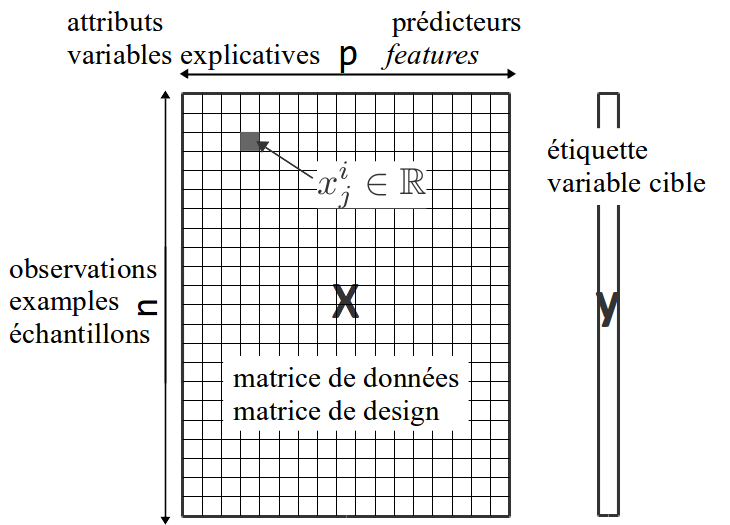
\includegraphics[width=0.7\textwidth]{figures/erm/suplearning}
%   \caption{Les donn�es d'un probl�me d'apprentissage supervis� sont organis�es
%     en une matrice de design et un vecteur d'�tiquettes. Les observations sont
%     repr�sent�es par leurs variables explicatives.}
%   \label{fig:suplearning}
% \end{figure}

\subsection{D�cision}
Dans le cas d'un probl�me de classification, le mod�le pr�dictif peut prendre
directement la forme d'une fonction $f$ � valeurs dans $\{0, 1\}$, ou utiliser
une fonction interm�diaire $g$ � valeurs r�elles, qui associe � une observation
un score d'autant plus �lev� qu'elle est susceptible d'�tre positive. Ce score
peut par exemple �tre la probabilit� que cette observation appartienne � la
classe positive. On obtient alors $f$ en {\it seuillant} $g$ ; $g$ est appel�e
{\it fonction de d�cision}.

% Dans le cadre d'un probl�me de classification binaire, on appelle {\it fonction
%   de d�cision}, ou {\it fonction discriminante}, une fonction
% $g:\XX \mapsto \RR$ telle que $f(\xx) = 0$ si et seulement si $g(\xx) \leq 0$
% et $f(\xx) = 1$ si et seulement si
% $g(\xx) > 0$. \\

% % Cette d�finition se g�n�ralise dans le cas de la classification {\it
% %   multi-classe} : on a alors $C$ fonctions de d�cision $g_c:\XX \mapsto \RR$
% % telles que $f(\xx) = \argmax_{c = 1, \dots, C} g_c(\xx).$

% Le concept de fonction de d�cision permet de partitionner l'espace en {\it
%   r�gions de d�cision} : \\
% Dans le cas d'un probl�me de classification binaire, la fonction discriminante
% partitionne l'espace des observations $\XX$ en deux {\it r�gions de d�cision},
% $\Rcal_0$ et $\Rcal_1$, telles que
% \begin{equation*}
%   \Rcal_0 = \{\xx \in \XX | g(\xx) \leq 0\} \text{ et }
%   \Rcal_1 = \{\xx \in \XX | g(\xx) > 0\}.
% \end{equation*}
% % Dans le cas multi-classe, on a alors $C$ r�gions de d�cision
% % \begin{equation*}
% %   \Rcal_c = \{\xx \in \XX | g_c(\xx) = \max_k g_k(\xx) \}.
% % \end{equation*}

% Les r�gions de d�cision sont s�par�es par des {\it fronti�res de d�cision} : \\
% Dans le cadre d'un probl�me de classification, on appelle {\it fronti�re de
%   d�cision}, ou {\it discriminant}, l'ensemble des points de $\XX$ o� une
% fonction de d�cision s'annule.  Dans le cas d'un probl�me binaire, il y a
% une seule fronti�re de d�cision ; dans le cas d'un probl�me multi-classe �
% $C$ classes, il y en a $C$.

\section{Espace des hypoth�ses}
Pour poser un probl�me d'apprentissage supervis�, il nous faut d�cider du
type de fonctions de mod�lisation que nous allons consid�rer. 

On appelle {\it espace des hypoth�ses} l'espace de fonctions
$\FF \subseteq \YY^\XX$ d�crivant les fonctions de mod�lisation que nous allons
consid�rer. Cet espace est choisi en fonction de nos {\it convictions} par
rapport au probl�me. 

\begin{exemple}
  Dans l'exemple de la figure~\ref{fig:simple_classif_pb}, on pourra d�cider de
  se restreindre � des discriminants qui soient des ellipses � axes parall�les
  aux axes de coordonn�es.  Ainsi, l'espace des hypoth�ses sera
  \begin{equation*}
    \FF = \{ \xx \mapsto \alpha (x_1-a)^2 + \beta (x_2-b)^2 - 1  \}.
  \end{equation*}
\end{exemple}
\begin{figure}[h]
  \centering
  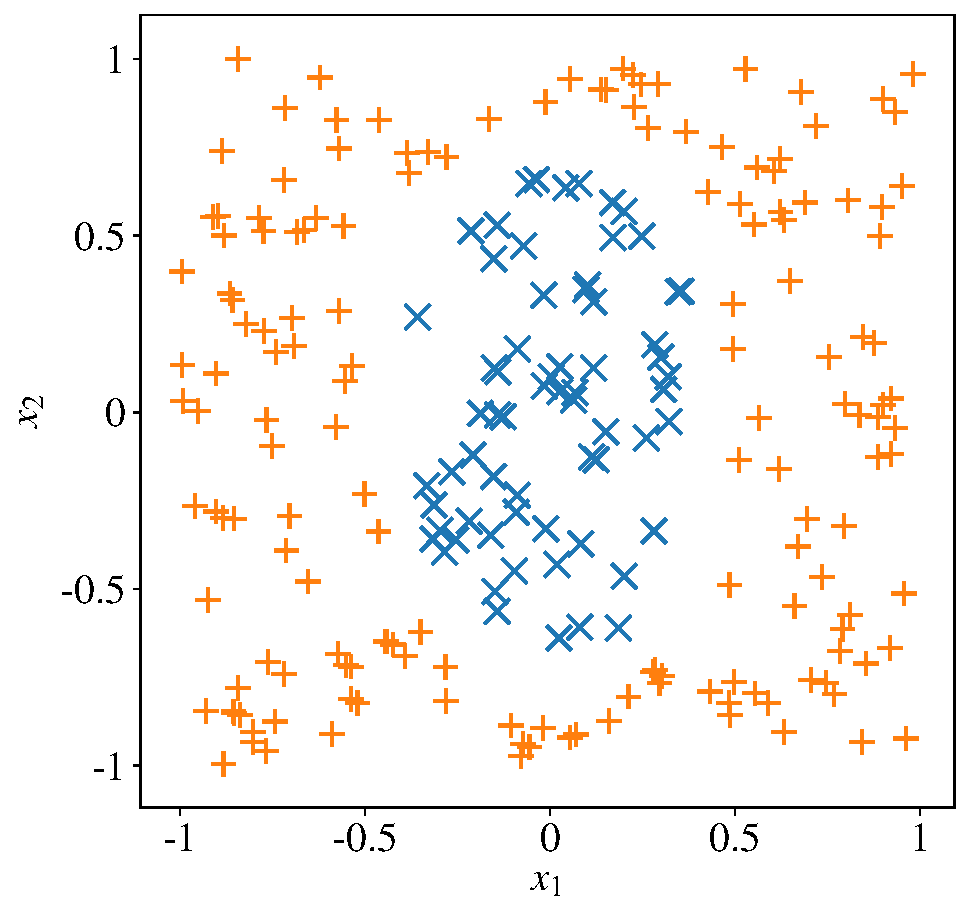
\includegraphics[width=0.5\textwidth]{figures/erm/simple_classif}
  \caption{Les exemples positifs (+) et n�gatifs (x) semblent �tre s�parables
    par une ellipse.}
  \label{fig:simple_classif_pb}
\end{figure}

�tant donn�s un jeu de $n$ observations �tiquet�es
$\DD = \{(\xx^i, y^i)\}_{i=1, \dots, n}$ et un espace d'hypoth�ses $\FF$.  La
t�che d'apprentissage supervis� consiste � supposer que les �tiquettes $y^i$
ont �t� calcul�es gr�ce � une fonction $\phi: \XX \rightarrow \YY$, et �
trouver une hypoth�se $f \in \FF$ qui approche au mieux la fonction cible
$\phi$.  Pour r�aliser une telle t�che, nous allons avoir alors besoin de deux
outils suppl�mentaires :
\begin{enumerate}
\item Une fa�on de {\it quantifier la qualit� d'une hypoth�se}, afin de
  pouvoir d�terminer si une hypoth�se satisfaisante (voire optimale) a �t�
  trouv�e.  Pour cela, nous allons d�finir dans la section~\ref{sec:losses}
  la notion de {\it fonction de co�t}.
\item Une fa�on de {\it chercher une hypoth�se optimale} dans $\FF$.  Dans
  cet ouvrage, nous allons nous concentrer sur les m�thodes
  d'\textit{apprentissage par optimisation} : les algorithmes d'apprentissage
  supervis� que nous allons �tudier auront pour but de trouver dans $\FF$
  l'hypoth�se optimale au sens de la fonction de co�t
  (cf. section~\ref{sec:mre}). Diff�rents algorithmes d�finiront diff�rents
  $\FF$, et selon les cas cette recherche sera exacte ou approch�e.
\end{enumerate}

Le choix de l'espace des hypoth�ses est fondamental.  En effet, si cet espace
ne contient pas la \og bonne \fg~fonction % , par exemple si l'on choisit comme
% espace des hypoth�ses pour les donn�es de la figure~\ref{fig:simple_classif_pb}
% l'ensemble des droites,
il sera impossible de trouver une bonne fonction de
d�cision.  Cependant, si l'espace est trop g�n�rique, il sera plus difficile et
intensif en temps de calcul d'y trouver une bonne fonction de mod�lisation.
  

\section{Minimisation du risque empirique}
\label{sec:mre}
R�soudre un probl�me d'apprentissage supervis� revient � trouver une fonction
$f \in \FF$ dont les pr�dictions soient les plus proches possibles des
v�ritables �tiquettes, sur tout l'espace $\XX$. On utilise pour formaliser cela
la notion de {\it fonction de co�t} :

Une {\it fonction de co�t} $L: \YY \times \YY \rightarrow \RR$, 
aussi appel�e {\it fonction de perte} ou {\it fonction d'erreur}
(en anglais : {\it cost function} ou {\it loss function})
est une fonction utilis�e pour quantifier la qualit� d'une pr�diction : 
$L(y, f(\xx))$ est d'autant plus grande que l'�tiquette $f(\xx)$ est �loign�e de
la vraie valeur $y$.


�tant donn�e une fonction de co�t $L$, nous cherchons donc $f$ qui minimise
ce co�t sur l'ensemble des valeurs possibles de $\xx \in \XX$, ce qui est
formalis� par la notion de {\it risque.}

Dans le cadre d'un probl�me d'apprentissage supervis�, on appelle {\it
  risque} l'esp�rance d'une fonction de co�t :
\begin{equation*}
  \Rcal(h) = \EE_{\XX}[L(h(\xx), y)].
\end{equation*}

La fonction $f$ que nous cherchons v�rifie donc $f = \argmin_{h \in \FF}
\EE[L(h(\xx), y)].$ Ce probl�me est g�n�ralement insoluble sans plus
d'hypoth�ses : si nous connaissions les �tiquettes de tous les points de
$\XX$, nous n'aurions pas besoin d'apprentissage automatique.  �tant donn�es
$n$ observations �tiquet�es $\{(\xx^i, y^i)\}_{i=1, \dots, n}$, on approchera
donc le risque par son estimation sur ces donn�es observ�es

Dans le cadre d'un probl�me d'apprentissage supervis�, �tant donn�es $n$
observations �tiquet�es $\{(\xx^i, y^i)\}_{i=1, \dots, n}$, on appelle {\it risque
  empirique} l'estimateur
\begin{equation*}
  R_n(h) = \frac{1}{n} \sum_{i=1}^n L(h(\xx^i), y^i).
\end{equation*}


Le pr�dicteur par {\it minimisation du risque empirique} est donc
\begin{equation}
  \label{eq:erm}
  f = \argmin_{h \in \FF} \frac{1}{n} \sum_{i=1}^n L(h(\xx^i), y^i).
\end{equation}

Selon le choix de $\FF$, l'�quation~\ref{eq:erm} peut avoir une solution
analytique explicite. Cela ne sera pas souvent le cas ; cependant on choisira
souvent une fonction de co�t {\it convexe} afin de r�soudre plus facilement ce
probl�me d'optimisation.

La minimisation du risque empirique est g�n�ralement un probl�me {\it mal pos�}
au sens de Hadamard, c'est-�-dire qu'il n'admet pas une solution unique
d�pendant de fa�on continue des conditions initiales. Il se peut par exemple
qu'un nombre infini de solutions minimise le risque empirique � z�ro (voir
figure~\ref{fig:multiple_solutions}).

\begin{figure}[h]
  \centering
  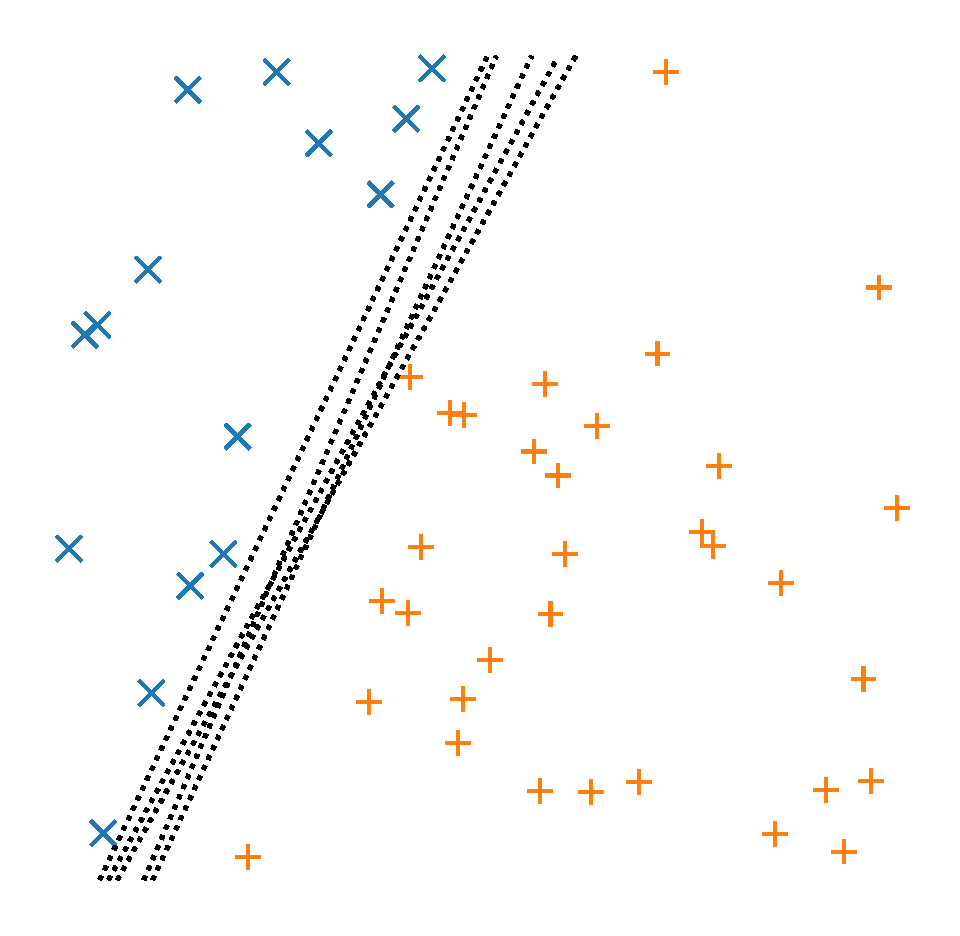
\includegraphics[width=0.5\textwidth]{figures/erm/multiple_solutions}
  \caption{Une infinit� de droites s�parent parfaitement les points positifs
    (+) des points n�gatifs (x). Chacune d'entre elles a un risque empirique
    nul.}
  \label{fig:multiple_solutions}
\end{figure}
\todo{Non-convergence de l'ERM}
% De plus, le pr�dicteur par minimisation du risque empirique n'est pas
% statistiquement consistant. Rappelons qu'un estimateur $\theta_n$ (d�pendant de
% $n$ observations) d'un param�tre $\theta$ est {\it consistant} s'il converge en
% probabilit� vers $\theta$ quand $n$ croit vers l'infini :
% \begin{equation}
%   \label{eq:statistical_consistency}
%   \forall \epsilon > 0, \lim_{n \rightarrow \infty} 
%   \PP(|\theta_n - \theta| \geq \epsilon) = 0.
% \end{equation}

% La loi des grands nombres nous garantit que le risque empirique converge vers
% le risque :
% \begin{equation}
%   \label{eq:risk_cvg}
%   \forall h \in \FF, R_n(h) \xrightarrow[n \rightarrow \infty]{} \Rcal(h).
% \end{equation}
% Cela ne suffit cependant pas � garantir que le minimum du risque empirique
% $\min_{h \in \FF} R_n(h)$ converge vers le minimum du risque. En effet, si
% $\FF$ est l'espace des fonctions mesurables, $\min_{h \in \FF} R_n(h)$ vaut
% g�n�ralement $0$, ce qui n'est pas le cas de $\Rcal(h).$ Il n'y a donc aucune
% garantie que la fonction $f_n$ qui minimise $R_n(h)$ soit un bon estimateur du
% minimiseur $f$ de $\Rcal(h)$.

% La consistance de la minimisation du risque empirique d�pend de l'espace des
% versions $\FF$. L'�tude de cette consistance est un des principaux �l�ments de
% la th�orie de l'apprentissage de Vapnik-Chervonenkis, qui d�passe largement le
% cadre de ce cours.


  
\section{Fonctions de co�t}
\label{sec:losses}
Il existe de nombreuses fonctions de co�t. Le choix d'une fonction de co�t
d�pend d'une part du probl�me en lui-m�me, autrement dit de ce que l'on trouve
pertinent pour le cas pratique consid�r�, et d'autre part de consid�rations
pratiques : peut-on ensuite r�soudre le probl�me d'optimisation qui r�sulte de
ce choix de fa�on suffisamment exacte et rapide~?%  Cette section pr�sente les
% fonctions de co�ts les plus couramment utilis�es et on pourra s'y r�f�rer tout
% au long de la lecture de cet ouvrage.

% \subsection{Fonctions de co�t pour la classification binaire}
% Pour d�finir des fonctions de co�t pour la classification binaire, on
% consid�rera souvent $\YY = \{-1, 1\}$. En effet, dans le cas d'une
% classification parfaite, le produit $y f(\xx)$ est alors �gal � $1$.

\subsection{Co�t 0/1 pour la classification binaire}
Dans le cas d'une fonction $f$ � valeurs binaires, on appelle {\it fonction de
  co�t 0/1}, ou {\it 0/1 loss}, la fonction suivante :
\begin{align*}
  L_{0/1} : \YY \times \YY & \rightarrow \RR \\
  y, f(\xx) & \mapsto
              \begin{cases}
                1 & \mbox{ si } f(\xx) \neq y \\
                0 & \mbox{ sinon.}
              \end{cases}
\end{align*}

En utilisant $\YY = \{-1, 1\}$, on peut la r��crire de la mani�re suivante :
\begin{equation*}
  L_{0/1}(y, f(\xx)) = \frac{1 - y f(\xx)}{2}.
\end{equation*}
Quand on utilise cette fonction de co�t, le risque empirique est le nombre
moyen d'erreurs de pr�diction.% \\

% Si l'on consid�re pour $f$ une fonction de d�cision (� valeurs r�elles) plut�t
% qu'une fonction de pr�diction � valeurs binaires, on peut d�finir la fonction
% de co�t 0/1 comme suit :
% \subsubsection{Co�t 0/1 pour la r�gression}
% Quand on consid�re une fonction de d�cision � valeurs r�elles, on appelle
% {\it fonction de co�t 0/1}, ou {\it 0/1 loss}, la fonction suivante :
% \begin{align*}
%   L_{0/1} : \YY \times \RR & \rightarrow \RR \\
%   y, f(\xx) & \mapsto
%               \begin{cases}
%                 1 & \mbox{ si } y f(\xx) \leq 0 \\
%                 0 & \mbox{ sinon.}
%               \end{cases}
% \end{align*}

% L'inconv�nient de cette fonction de co�t est qu'elle n'est pas d�rivable, ce
% qui compliquera les probl�mes d'optimisation l'utilisant. De plus, elle n'est
% pas tr�s fine : l'erreur est la m�me que $f(\xx)$ soit tr�s proche ou tr�s loin
% du seuil de d�cision.  Rappelons que pour une classification parfaite, quand
% $\YY = \{-1, 1\}$, $y f(\xx) = 1$. On peut ainsi d�finir une fonction de co�t
% qui soit d'autant plus grande que $y f(\xx)$ s'�loigne de $1$ � gauche ; on
% consid�re qu'il n'y a pas d'erreur si $y f(\xx) > 1$. Cela conduit � la
% d�finition d'erreur {\it hinge}, ainsi appel�e car elle forme un coude, ou une
% charni�re (cf. figure~\ref{fig:classif_losses}).

% \subsubsection{Erreur hinge}
% \label{sec:hinge-loss}
% On appelle {\it fonction d'erreur hinge}, ou {\it hinge loss}, la fonction
% suivante :
% \begin{align*}
%   L_{\text{hinge}} : \{-1, 1\} \times \RR & \rightarrow \RR \\
%   y, f(\xx) & \mapsto
%               \begin{cases}
%                 0 & \mbox{ si } y f(\xx) \geq 1 \\
%                 1 - y f(\xx) & \mbox{ sinon.}
%               \end{cases}
% \end{align*}
% De mani�re plus compacte, l'erreur hinge peut aussi s'�crire 
% \begin{equation*}
%   \label{eq:hinge-loss}
%   L_{\text{hinge}}(f(\xx), y) = \max\left(0, 1 - y f(\xx) \right) = \left[ 1 - y f(\xx)\right]_+. 
% \end{equation*}

% On peut aussi consid�rer que $f(\xx)$ doit �tre la plus proche possible de $1$
% pour les observations positives (et $-1$ pour les observations
% n�gatives). Ainsi, on p�nalisera aussi les cas o� $y f(\xx)$ s'�loigne de $1$
% par la droite, ce que l'on peut faire avec le {\it co�t quadratique}.

% \subsubsection{Co�t quadratique pour la classification binaire}
% Dans le cadre d'un probl�me de classification binaire, on appelle {\it co�t
%   quadratique}, ou {\it square loss}, la fonction suivante :
% \begin{align*}
%   L_{\text{square}} : \{-1, 1\} \times \RR & \rightarrow \RR \\
%   y, f(\xx) & \mapsto  \left( 1 -y f(\xx)\right)^2.
% \end{align*}

% Enfin, on peut chercher � d�finir une fonction de d�cision dont la valeur
% absolue quantifie notre confiance en sa pr�diction. On cherche alors � ce que
% $y f(\xx)$ soit la plus grande possible, et on utilise le {\it co�t
%   logistique}.

\subsection{Co�t logistique et entropie crois�e}
\label{sec:logistic_loss}
On appelle {\it fonction de co�t logistique}, ou {\it logistic loss}, la
fonction suivante :
\begin{align*}
  L_{\log} : \{-1, 1\} \times \RR & \rightarrow \RR \\
  y, f(\xx) & \mapsto \log \left( 1 + \exp(-y f(\xx))\right).
\end{align*}

Si l'on pr�f�re utiliser $\YY = \{0, 1\}$, le co�t logistique est �quivalent �
l'{\it entropie crois�e}.

\label{sec:cross_entropy}
Dans le cas binaire, on appelle {\it entropie crois�e}, ou {\it cross-entropy},
la fonction suivante :
\begin{align*}
  L_H : \{0, 1\} \times ]0, 1[ & \rightarrow \RR \\
  y, f(\xx) & \mapsto - y \log f(\xx) - (1-y) \log(1-f(\xx)).
\end{align*}

L'entropie crois�e est issue de la th�orie de l'information, d'o� son nom. En
consid�rant que la v�ritable classe de $\xx$ est mod�lis�e par une distribution
$Q$, et sa classe pr�dite par une distribution $P$, nous allons chercher �
mod�liser $P$ de sorte qu'elle soit la plus proche possible de $Q$. On utilise
pour cela la {\it divergence de Kullback-Leibler}:
\begin{align*}
  KL(Q||P) & = \sum_{c=0, 1} Q(y=c|\xx) \log \frac{Q(y=c|\xx)}{P(y=c|\xx)} \\
           & = - \sum_{c=0, 1} Q(y=c|\xx) \log P(y=c|\xx) + 
             \sum_{c=0, 1} Q(y=c|\xx) \log Q(y=c|\xx)
\end{align*}
Comme $Q(y=c|\xx)$ vaut soit $0$ ($c$ n'est pas la classe de $\xx$) soit
$1$ (dans le cas contraire), le deuxi�me terme de cette expression est nul
et on retrouve ainsi la d�finition ci-dessus de l'entropie crois�e.


% Les fonctions de perte pour la classification binaire sont illustr�es sur la
% figure~\ref{fig:classif_losses}.
% \begin{figure}[h]
%   \centering
%   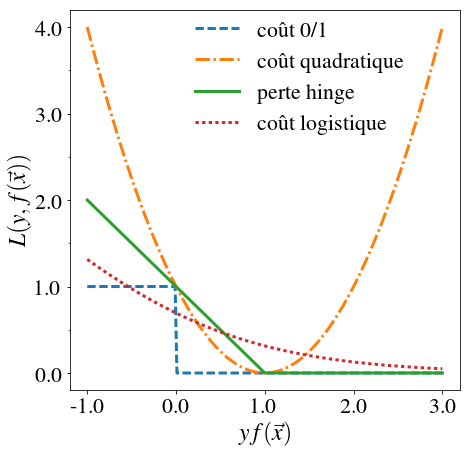
\includegraphics[width=0.7\textwidth]{figures/erm/classif_losses}
%   \caption{Fonctions de perte pour la classification binaire.}
%   \label{fig:classif_losses}
% \end{figure}

% \subsection{Co�ts pour la r�gression}
% Dans le cas d'un probl�me de r�gression, nous consid�rons maintenant
% $\YY=\RR.$ Le but de notre fonction de co�t est de p�naliser les fonctions de
% pr�diction $f$ dont la valeur est �loign�e de la valeur cible $\xx$.
\subsection{Co�t quadratique pour la r�gression}
\label{sec:quadratic_loss}
On appelle {\it fonction de co�t quadratique}, ou {\it quadratic loss}, ou
encore {\it squared error}, la fonction suivante :
\begin{align*}
  L_{\text{SE}} : \RR \times \RR & \rightarrow \RR \\
  y, f(\xx) & \mapsto \frac{1}{2} \left(y - f(\xx)\right)^2.
\end{align*}
Le coefficient $\frac{1}{2}$ permet d'�viter d'avoir des coefficients
multiplicateurs quand on d�rive le risque empirique pour le minimiser.

% \subsubsection{Co�t $\epsilon$-insensible}
% \label{sec:epsilon_insensitive}
% Le co�t quadratique a tendance � �tre domin� par les valeurs aberrantes : d�s
% que quelques observations dans le jeu de donn�es ont une pr�diction tr�s
% �loign�e de leur �tiquette r�elle, la qualit� de la pr�diction sur les autres
% observations importe peu. On peut ainsi lui pr�f�rer le {\it co�t absolu} : \\

% On appelle {\it fonction de co�t absolu}, ou {\it absolute error}, la fonction
% suivante :
% \begin{align*}
%   L_{\text{AE}} : \RR \times \RR & \rightarrow \RR \\
%   y, f(\xx) & \mapsto  |y - f(\xx)|.
% \end{align*}

% Avec cette fonction de co�t, m�me les pr�dictions tr�s proches de la v�ritable
% �tiquette sont p�nalis�es (m�me si elles le sont faiblement). Cependant, il est
% num�riquement quasiment impossible d'avoir une pr�diction exacte. Le co�t {\it
%   $\epsilon$-insensible} permet de rem�dier � cette limitation.

% �tant donn� $\epsilon > 0$, on appelle {\it fonction de co�t
%   $\epsilon$-insensible}, ou {\it $\epsilon$-insensitive loss}, la fonction
% suivante :
% \begin{align*}
%   L_\epsilon : \RR \times \RR & \rightarrow \RR \\
%   y, f(\xx) & \mapsto \max \left(0, |y - f(\xx)| - \epsilon\right).
% \end{align*}
    
% \subsubsection{Co�t de Huber}
% Le co�t $\epsilon$-insensible n'est d�rivable ni en $-\epsilon$ ni en
% $+\epsilon$, ce qui complique l'optimisation du risque empirique.  La {\it
%   fonction de co�t de Huber} permet d'�tablir un bon compromis entre le co�t
% quadratique (d�rivable en $0$) et le co�t absolu (qui n'explose pas dans les
% valeurs extr�mes).

% On appelle {\it fonction de co�t de Huber}, ou {\it Huber loss}, la fonction
% suivante :
% \begin{align*}
%   L_{\text{Huber}} : \RR \times \RR & \rightarrow \RR \\
%   y, f(\xx) & \mapsto
%               \begin{cases}
%                 \frac{1}{2} \left(y - f(\xx)\right)^2 & \text{ si } |y - f(\xx)| < \epsilon \\
%                 \epsilon |y - f(\xx)| - \frac{1}{2} \epsilon^2 & \text{ sinon.} 
%               \end{cases}
% \end{align*}
% Le terme $- \frac{1}{2} \epsilon^2$ permet d'assurer la continuit� de la fonction.\\

% Les fonctions de co�t pour la r�gression sont illustr�es sur la
% figure~\ref{fig:regression_losses}.

% \begin{figure}[h]
%   \centering
%   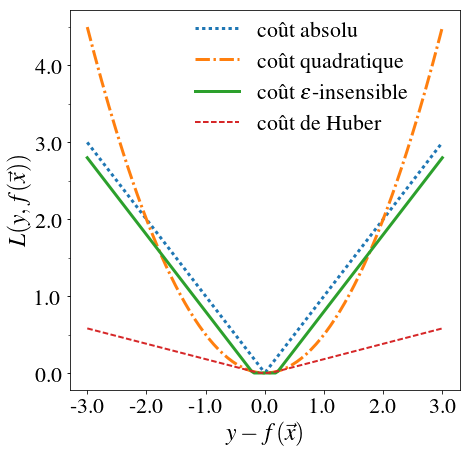
\includegraphics[width=0.7\textwidth]{figures/erm/regression_losses}
%   \caption{Fonctions de co�t pour un probl�me de r�gression.}
%   \label{fig:regression_losses}
% \end{figure}



\section{Apprentissage supervis� d'un mod�le param�trique}
\subsection{Mod�les param�triques}
On parle de {\it mod�le param�trique} quand on utilise un algorithme
d'apprentissage dont le but est de trouver les valeurs optimales des param�tres
d'un mod�le dont on a d�fini la forme analytique en fonction des descripteurs.

La complexit� d'un mod�le param�trique grandit avec le nombre de param�tres �
apprendre, autrement dit avec le nombre de variables. � l'inverse, la
complexit� d'un mod�le non param�trique aura tendance � grandir avec le nombre
d'observations.

Par exemple, un algorithme d'apprentissage qui permet d'apprendre les
coefficient $\alpha$, $\beta$, $\gamma$ dans la fonction de d�cision suivante :
$f: \xx \mapsto \alpha x_1 + \beta x_2x_4^2 + \gamma e^{x_3-x_5}$ apprend un
mod�le param�trique. Quel que soit le nombre d'observations, ce mod�le ne
change pas.

� l'inverse, la m�thode du plus proche voisin, qui associe � $\xx$ l'�tiquette
du point du jeu d'entra�nement dont il est le plus proche en distance
euclidienne, apprend un mod�le non param�trique : on ne sait pas �crire la
fonction de d�cision comme une fonction des variables pr�dictives. Plus il y a
d'observations, plus le mod�le pourra apprendre une fronti�re de d�cision
complexe.

�tant donn� un jeu $\DD = \{\xx^i, y^i\}_{i=1, \dots, n}$ de $n$ observations
en $p$ dimensions et leurs �tiquettes r�elles, nous supposons ici que la
fonction de d�cision $f$ est param�tr�e par le vecteur
$\bbeta \in \mathbb{R}^{m}$.

Nous allons faire l'hypoth�se que les erreurs, c'est-�-dire la diff�rence entre
les �tiquettes r�elles et les valeurs correspondantes de $f$, sont normalement
distribu�es, centr�es en $0:$
\begin{equation}
  \label{eq:linreg_gaussian_error}
  y = f(\xx|\bbeta) + \epsilon \hspace{2em} \epsilon \sim \Ncal(0, \sigma^2).
\end{equation}
Cette hypoth�se est illustr�e sur la figure~\ref{fig:linreg} dans le cas
d'une fonction de d�cision lin�aire.

\begin{figure}[h]
  \centering
  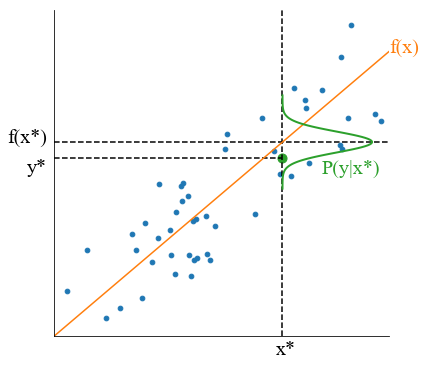
\includegraphics[width=0.7\textwidth]{figures/erm/linreg}
  \caption{Pour une observation $x^*$ donn�e (ici en une dimension) , la
    distribution des valeurs possibles de l'�tiquette $y^*$ correspondante est
    une gaussienne centr�e en $f(x^*)$.}
  \label{fig:linreg}
\end{figure}

Selon cette hypoth�se, les observations $\xx$ sont la r�alisation de $p$
variables al�atoires $X_1, X_2, \dots, X_p$ � valeurs r�elles, leurs �tiquettes
$y$ sont la r�alisation d'une variable al�atoire $Y$ � valeurs r�elles, et ces
variables al�atoires v�rifient
\begin{equation}
  \label{eq:linreg_bayes}
  \PP(Y=y|X = \xx) \sim 
  \Ncal\left(f(\xx|\bbeta), \sigma^2\right).
\end{equation}
On note ici $\PP(X=\xx)$ pour
$\PP(X_1=x_1, X_2=x_2, \dots, X_p=x_p).$

\subsection{Estimation par maximum de vraisemblance et m�thode des
  moindres carr�s}
\label{sec:least_squares}
Sous l'hypoth�se~\ref{eq:linreg_bayes}, et en supposant les $n$ observations
ind�pendantes et identiquement distribu�es, le log de vraisemblance du
param�tre $\bbeta$ vaut:
\begin{align*}
  \log \PP(\DD|\bbeta) & = \log \prod_{i=1}^n \PP(X = \xx^i|\bbeta) \\
                       & = \log \prod_{i=1}^n \PP(y^i|\xx^i) + \log \prod_{i=1}^n
                         \PP(X = \xx^i) \\
                       & = - \log \frac1{2\sigma^2} \sum_{i=1}^n \left(y^i -
                         f(\xx^i|\bbeta) \right)^2 + \Ccal
\end{align*}
Dans cette derni�re �quation, $\Ccal$ est une constante par rapport � $\bbeta$,
et provient d'une part du coefficient $\frac1{\sqrt{2\pi}}$ de la distribution
normale et d'autre part des $\PP(X=\xx^i).$

Ainsi, maximiser la vraisemblance revient � minimiser
$\sum_{i=1}^n \left(y^i - f(\xx^i|\bbeta) \right)^2$ : c'est ce que l'on
appelle la {\it minimisation des moindres carr�s}, une m�thode bien connue
depuis Gauss et Legendre. Notons aussi que cela revient � minimiser le risque
empirique quand il est d�fini en utilisant la fonction de co�t
quadratique~\ref{sec:quadratic_loss}.

\section{R�gression lin�aire}
Commen�ons par consid�rer des mod�les {\it lin�aires}: nous cherchons �
expliquer la variable cible $y$ par une {\it combinaison lin�aire} -- en
d'autres mots une somme pond�r�e -- des descripteurs.

\subsection{Formulation}
Nous choisissons une fonction de d�cision $f$ de la forme
\begin{equation}
  \label{eq:linear_decision}
  f: \xx \mapsto \beta_0 + \sum_{j=1}^p \beta_j x_j.
\end{equation}
Ici, $\bbeta \in \RR^{p+1}$ et donc $m=p+1$.

\subsection{Solution}
On appelle {\it r�gression lin�aire} le mod�le de la forme
$f: \xx \mapsto \beta_0 + \sum_{j=1}^p \beta_j x_j$ dont les coefficients sont
obtenus par minimisation de la somme des moindres carr�s, � savoir :
\begin{equation}
  \label{eq:linreg}
  \argmin_{\bbeta \in \RR^{p+1}}  \sum_{i=1}^n \left(y^i - \left(\beta_0 + 
      \sum_{j=1}^p \beta_j x_j \right)\right)^2.
\end{equation}
  
Nous pouvons r��crire le probl�me~\ref{eq:linreg} sous forme matricielle, en
ajoutant � gauche � la matrice d'observations $X \in \RR^p$ une colonne de 1 :
\begin{equation}
  \label{eq:added_ones}
  X \leftarrow   \begin{pmatrix}
    1 & x_1^1 & \cdots & x_p^1 \\
    \vdots & \vdots & \cdots & \vdots \\
    1 & x_1^n& \cdots & x_p^n \\
  \end{pmatrix}.
\end{equation}

La somme des moindres carr�s s'�crit alors
\begin{equation}
  \label{eq:rss_linreg}
  \text{RSS} = \left(\yy - X \bbeta\right)^\top \left(\yy -  X \bbeta\right).
\end{equation}

Il s'agit d'une forme quadratique convexe en $\bbeta$, que l'on peut donc
minimiser en annulant son gradient
$\nabla_{\bbeta} \text{RSS} = -2 X^\top \left(\yy - X \bbeta \right)$. On
obtient alors
\begin{equation}
  \label{eq:linreg_sol}
  X^\top X \bbeta^* = X^\top \yy.
\end{equation}
  
Si le rang de la matrice $X$ est �gal � son nombre de colonnes, alors la
somme des moindres carr�s~\ref{eq:rss_linreg} est minimis�e pour
\begin{equation*}
  \bbeta^* = \left(X^\top X \right)^{-1} X^\top \yy.
\end{equation*}

Preuve :  Si $X$ est de rang colonne plein, alors $X^\top X$ est inversible.\\
  
Si $X^\top X$ n'est pas inversible, on pourra n�anmoins trouver une solution
(non unique) pour $\bbeta$ en utilisant � la place de
$\left(X^\top X \right)^{-1}$ un pseudo-inverse (par exemple, celui de
Moore-Penrose) de $X^\top X$, c'est-�-dire une matrice $M$ telle que
$X^\top X M X^\top X = X^\top X.$

On peut aussi (et ce sera pr�f�rable quand $p$ est grand et que l'inversion de
la matrice $X^\top X \in \RR^{p \times p}$ est donc co�teuse) obtenir une
estimation de $\bbeta$ par un algorithme � directions de descente.

On fera attention � ne pas confondre les {\it variables}, qui sont les $p$
valeurs $x_1, x_2, \dots, x_p$ qui d�crivent les donn�es, et les {\it
  param�tres}, qui sont les $p+1$ valeurs $\beta_0, \beta_1, \dots, \beta_p$
qui param�trent le mod�le.

La r�gression lin�aire produit un mod�le interpr�table, au sens o� les
$\beta_j$ permettent de comprendre l'importance relative des variables sur la
pr�diction. En effet, plus $\lvert \beta_j \rvert$ est grande, plus la $j$-�me
variable a un effet important sur la pr�diction, et le signe de $\beta_j$ nous
indique la direction de cet effet.

Attention ! Cette interpr�tation n'est valide que si les variables ne sont pas
corr�l�es, et que $x_j$ peut �tre modifi�e sans perturber les autres
variables. De plus, si les variables sont corr�l�es, $X$ n'est pas de rang
colonne plein et $X^\top X$ n'est donc pas inversible. Ainsi la r�gression
lin�aire admet plusieurs solutions. Intuitivement, on peut passer de l'une �
l'autre de ces solutions car une perturbation d'un des poids $\beta_j$ peut
�tre compens�e en modifiant les poids des variables corr�l�es � $x_j$.





  
% \section{Points cl�s}
% \begin{itemize}
% \item Les trois ingr�dients d'un algorithme d'apprentissage supervis� sont :
%   \begin{itemize}
%   \item l'espace des hypoth�ses,
%   \item la fonction de co�t,
%   \item l'algorithme d'optimisation qui permet de trouver l'hypoth�se
%     optimale au sens de la fonction de co�t sur les donn�es (minimisation du
%     risque empirique).
%   \end{itemize}
% \item On peut apprendre les coefficients d'un mod�le de r�gression param�trique
%   par maximisation de vraisemblance, ce qui �quivaut � minimiser le risque
%   empirique en utilisant le co�t quadratique comme fonction de perte, et
%   revient � la m�thode des moindres carr�s.
% \item La r�gression lin�aire admet une unique solution $\bbeta^* = \left(X^\top
%     X \right)^{-1} X^\top \yy$ si et seulement si $X^\top X$ est
%   inversible. Dans le cas contraire, il existe une infinit� de solutions.

% \end{itemize}


% % \begin{plusloin}
% % \item La notion de complexit� d'un mod�le a �t� formalis�e par Vladimir Vapnik et
% %   Alexey Chervonenkis dans les ann�es 1970, et est d�taill�e par exemple
% %   dans l'ouvrage de \citet{vapnik1995}.
% % \item Pour en savoir plus sur la th�orie de l'apprentissage, on pourra se
% %   r�f�rer au livre de \citet{kearns1994}.
% % \item On trouvera une discussion d�taill�e du compromis biais-variance dans
% %   \citet{friedman1997}.
% % \end{plusloin}

% % \section*{Bibliographie}
% % \vspace{-25pt}
% % \begin{thebibliography}{99}
% % \bibitem[\protect\astroncite{Crammer and Singer}{2001}]{crammer2001}
% % Crammer, K. and Singer, Y. (2001).
% % \newblock On the algorithmic implementation of multiclass kernel-based vector
% %   machines.
% % \newblock {\em Journal of Machine Learning Research}, 2:265--292.

% % \bibitem[\protect\astroncite{Friedman}{1997}]{friedman1997} Friedman,
% %   J.~H. (1997).  \newblock On bias, variance, 0/1-loss and the curse of
% %   dimensionality.  \newblock {\em Data Mining and Knowledge Discovery},
% %   1:55--77.

% % \bibitem[\protect\astroncite{Kearns et Vazirani}{1994}]{kearns1994} Kearns,
% %   M.~J. et Vazirani, U.~V. (1994).  \newblock {\em An Introduction to
% %     Computational Learning Theory}.  \newblock MIT Press, Cambridge, MA.

% % \bibitem[\protect\astroncite{Vapnik}{1995}]{vapnik1995} Vapnik, V.~N. (1995).
% %   \newblock {\em The Nature of Statistical Learning Theory}.  \newblock
% %   Springer, New York.

% % \bibitem[\protect\astroncite{Weston and Watkins}{1999}]{weston1999}
% % Weston, J. and Watkins, C. (1999).
% % \newblock Support vector machines for multi-class pattern recognition.
% % \newblock In {\em European Symposium on Artificial Neural Networks}.
% % \end{thebibliography}



%%% Local Variables:
%%% mode: latex
%%% TeX-master: "sdd_2020_poly"
%%% End:
% \clearpage 

% \chapter{G�n�ralisation}
% %-*- coding: iso-latin-1 -*-    
\label{chap:generalisation}

\todo{
  \begin{itemize}
  \item Coh�rence des notations avec les chapitres pr�c�dents.
  \item Lien avec le cours d'optimisation.
  \item All�ger / �laguer.
  \end{itemize}
}


\paragraph{Notions :} g�n�ralisation ; sur-apprentissage ; s�lection de mod�le
; validation crois�e ; r�gularisation des mod�les param�triques lin�aires
\paragraph{Objectifs p�dagogiques :} 
\begin{itemize}      
  \setlength{\itemsep}{3pt}
\item D�tecter un risque de sur-apprentissage ;
\item Mettre en place un cadre permettant de s�lectionner un mod�le parmi
  plusieurs et d'estimer sa performance en g�n�ralisation ;
\item Utiliser la r�gularisation pour �viter le sur-apprentissage ;
\item Manipuler les r�gularisations $\ell_1$ et $\ell_2$ sur des mod�les lin�aires.
\end{itemize}

\section{G�n�ralisation et sur-apprentissage}
\subsection{G�n�ralisation}
Imaginons un algorithme qui, pour pr�dire l'�tiquette d'une observation $\xx$,
retourne son �tiquette si $\xx$ appartient aux donn�es dont l'�tiquette est
connue, et une valeur al�atoire sinon. Cet algorithme aura une erreur empirique
minimale quelle que soit la fonction de co�t choisie, mais fera de tr�s
mauvaises pr�dictions pour toute nouvelle observation. Ce n'est pas vraiment ce
que l'on a en t�te quand on parle d'{\it apprentissage}.

Ainsi, �valuer un algorithme de machine learning sur les donn�es sur lesquelles
il a appris ne nous permet absolument pas de savoir comment il se comportera
sur de nouvelles donn�es, en d'autres mots, sa capacit� de {\it
  g�n�ralisation}. C'est un point essentiel !

On appelle {\it g�n�ralisation} la capacit� d'un mod�le � faire des pr�dictions
correctes sur de nouvelles donn�es, qui n'ont pas �t� utilis�es pour le
construire.

\subsection{Sur-apprentissage}
L'exemple, certes extr�me, que nous avons pris plus haut, illustre que l'on
peut facilement mettre au point une proc�dure d'apprentissage qui produise un
mod�le qui fait de bonnes pr�dictions sur les donn�es utilis�es pour le
construire, mais g�n�ralise mal.  Au lieu de mod�liser la vraie nature des
objets qui nous int�ressent, un tel mod�le capture aussi (voire surtout) un
bruit qui n'est pas pertinent pour l'application consid�r�e. En effet, dans
tout probl�me d'apprentissage automatique, nos donn�es sont in�vitablement
bruit�es
\begin{itemize}
\item par des {\it erreurs de mesure} dues � la faillibilit� des capteurs
  utilis�s pour mesurer les variables par lesquelles on repr�sente nos donn�es,
  ou � la faillibilit� des op�rateurs humains qui ont entr� ces mesures dans
  une base de donn�es ;
\item par des {\it erreurs d'�tiquetage} (souvent appel�s {\it teacher's noise}
  en anglais) dues � la faillibilit� des op�rateurs humains qui ont �tiquet�
  les donn�es ;
\item enfin, parce que les variables mesur�es ne suffisent pas � mod�liser le
  ph�nom�ne qui nous int�resse, soit qu'on ne les connaisse pas, soit qu'elles
  soient co�teuses � mesurer.
\end{itemize}

Supposons que nous voulions classifier des photographies selon qu'elles
repr�sentent des pandas ou non. Chaque image est repr�sent�e par les valeurs
RGB des pixels qui la composent.  Nous aimerions faire en sorte que le mod�le
que nous construisons capture la v�ritable nature d'un panda. Nous pouvons
cependant �tre expos�s � des erreurs de mesure (erreurs techniques des capteurs
de l'appareil photo) ainsi que des erreurs d'�tiquetage (erreurs de la personne
qui a d� d�cider, pour chaque photo, s'il s'agissait ou non d'un panda, et a pu
cliquer sur le mauvais choix, ou confondre un panda avec un ours). De plus,
nous sommes limit�s par notre choix de variables : nos pixels ne capturent pas
directement le fait qu'un panda est un animal rondouillard, avec un masque
autour des yeux, g�n�ralement entour� de bambous.

On voit ici que le choix des variables utilis�es pour repr�senter les donn�es
est une �tape tr�s importante du processus de mod�lisation. Les techniques
pr�sent�es de r�duction de dimension que nous avons vues au
chapitre~\ref{chap:dimred} peuvent �tre utilis�es pour guider le choix des
variables pr�dictives � utiliser.

On dit d'un mod�le qui, plut�t que de capturer la nature des objets �
�tiqueter, mod�lise aussi le bruit et ne sera pas en mesure de g�n�raliser
qu'il {\it sur-apprend}. En anglais, on parle d'{\it overfitting}.

Un mod�le qui sur-apprend est g�n�ralement un mod�le {\it trop complexe}, qui
\og colle \fg~trop aux donn�es et capture donc aussi leur bruit.
  
� l'inverse, il est aussi possible de construire un mod�le {\it trop simple},
dont les performances ne soient bonnes ni sur les donn�es utilis�es pour le
construire, ni en g�n�ralisation.

On dit d'un mod�le qui est trop simple pour avoir de bonnes performances m�me
sur les donn�es utilis�es pour le construire qu'il {\it sous-apprend}. En
anglais, on parle d'{\it underfitting}.

Ces concepts sont illustr�s sur la figure~\ref{fig:overfit_class} pour un
probl�me de classification binaire et la figure~\ref{fig:overfit_regr} pour un
probl�me de r�gression.

\begin{figure}[h]
  \begin{subfigure}[t]{0.48\textwidth}
    \centering
    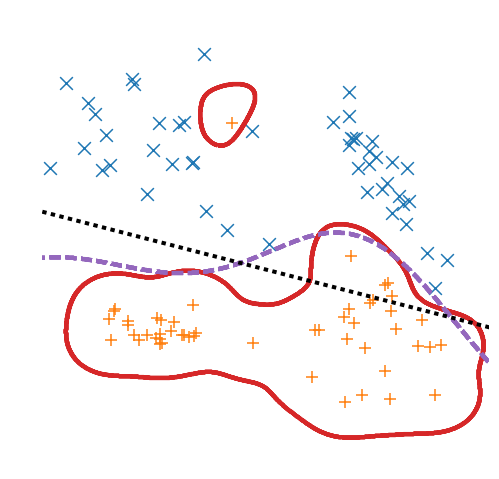
\includegraphics[width=\textwidth]{figures/generalisation/overfit_class}
    \caption{Pour s�parer les observations n�gatives (x) des observations
      positives (+), la droite pointill�e sous-apprend. La fronti�re de
      s�paration en trait plein ne fait aucune erreur sur les donn�es mais est
      susceptible de sur-apprendre. La fronti�re de s�paration en trait
      discontinu est un bon compromis.}
    \label{fig:overfit_class}
  \end{subfigure}
  \hfill
  \begin{subfigure}[t]{0.48\textwidth}
    \centering
    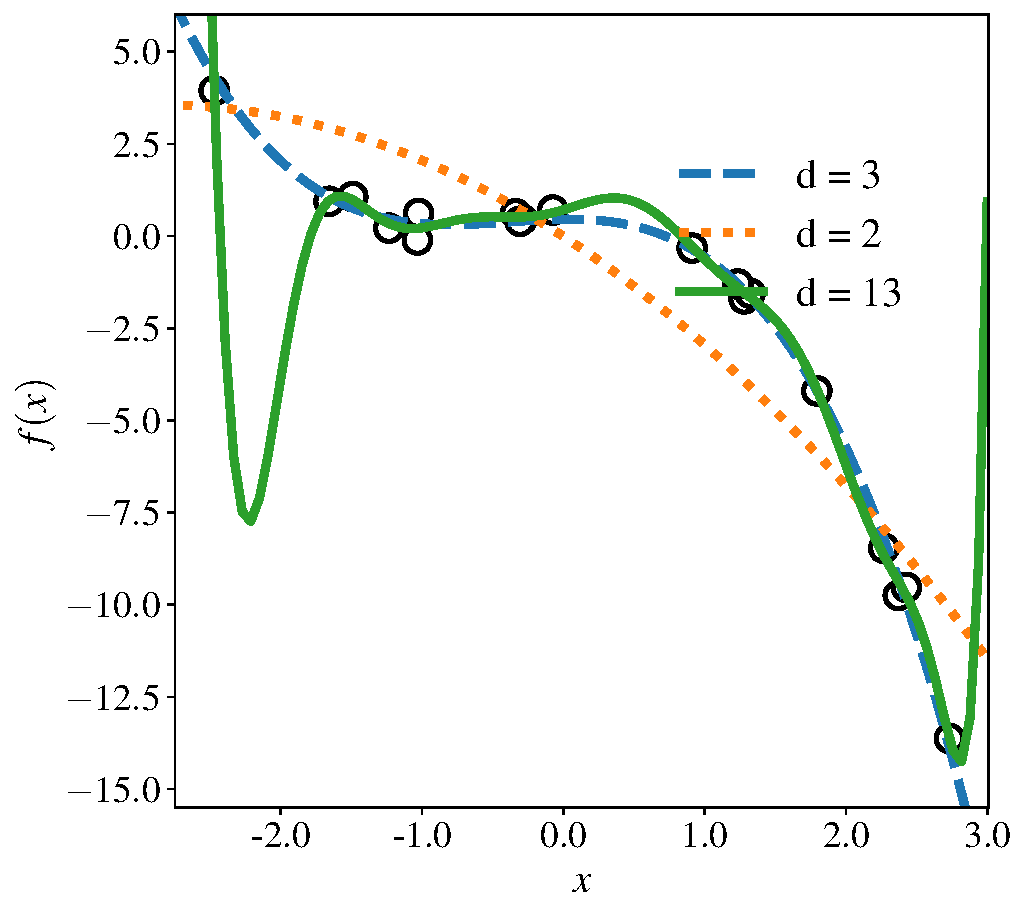
\includegraphics[width=\textwidth]{figures/generalisation/overfit_regr}
    \caption{Les �tiquettes $y$ des observations (repr�sent�es par des points)
      ont �t� g�n�r�es � partir d'un polyn�me de degr� $d=3$. Le mod�le de
      degr� $d=2$ approxime tr�s mal les donn�es et sous-apprend, tandis que
      celui de degr� $d=13$, dont le risque empirique est plus faible,
      sur-apprend.}
    \label{fig:overfit_regr}
  \end{subfigure}
  \caption{Sous-apprentissage et sur-apprentissage}
\end{figure}

\subsection{Compromis biais-variance}
\label{sec:bias_variance}
\todo{R��crire en lien avec le chapitre sur l'estimation.}
% Pour mieux comprendre le risque d'un mod�le $f: \XX \rightarrow \YY$, nous
% pouvons le comparer � l'erreur minimale $\Rcal^*$ qui peut �tre atteinte par
% n'importe quelle fonction mesurable de $\XX$ dans $\YY$ : c'est ce qu'on
% appelle l'\textit{exc�s d'erreur}, et que l'on peut d�composer de la fa�on
% suivante :
% \begin{equation}
%   \label{eq:estimation_approximation}
%   \Rcal(f) - \Rcal^* = \left[ \Rcal(f) - \min_{h \in \FF} 
%     \Rcal(h) \right]
%   + \left[ \min_{h \in \FF} \Rcal(h) - \Rcal^* \right]
% \end{equation}

% Le premier terme, $\Rcal(f) - \min_{h \in \FF} \Rcal(h)$, quantifie la distance
% entre le mod�le $f$ et le mod�le optimal sur $\FF$. C'est ce que l'on appelle
% {\it l'erreur d'estimation.}

% Le second terme, $\min_{h \in \FF} \Rcal(h) - \Rcal^*$, quantifie la qualit� du
% mod�le optimal sur $\FF$, autrement dit, la qualit� du choix de l'espace des
% hypoth�ses. C'est ce que l'on appelle {\it l'erreur d'approximation.} Si $\FF$
% est l'ensemble des fonctions mesurables, alors l'erreur d'approximation est
% nulle.

% Ainsi, l'�criture~\ref{eq:estimation_approximation} permet de d�composer
% l'erreur entre un terme qui d�coule de la qualit� de l'espace des hypoth�ses et
% un autre qui d�coule de la qualit� de la proc�dure d'optimisation utilis�e. En
% pratique, sauf dans des cas tr�s particuliers o� cela est rendu possible par
% construction, il n'est pas possible de calculer ces termes d'erreur.
% Cependant, cette �criture nous permet de comprendre le probl�me suivant :
% choisir un espace des hypoth�ses plus large permet g�n�ralement de r�duire
% l'erreur d'approximation, car un mod�le plus proche de la r�alit� a plus de
% chances de se trouver dans cet espace. Cependant, puisque cet espace est plus
% vaste, la solution optimale y est aussi g�n�ralement plus difficile � trouver :
% l'erreur d'estimation, elle, augmente. C'est dans ce cas qu'il y a
% sur-apprentissage. \\

Un espace des hypoth�ses plus large permet g�n�ralement de construire des
mod�les plus complexes : par exemple, l'ensemble des droites vs. l'ensemble des
polyn�mes de degr� 9 (cf. figure~\ref{fig:overfit_regr}). C'est une variante du
principe du {\it rasoir d'Ockham}, selon lequel les
hypoth�ses les plus simples sont les plus vraisemblables.

Il y a donc un compromis entre erreur d'approximation et erreur d'estimation :
il est difficile de r�duire l'une sans augmenter l'autre. Ce compromis est
g�n�ralement appel� {\it compromis biais-variance} : l'erreur d'approximation
correspond au {\it biais} de la proc�dure d'apprentissage, tandis que l'erreur
d'estimation correspond � sa {\it variance}. % On retrouvera ce compromis dans
% l'estimation bay�sienne de param�tres � la
% section~\ref{sec:bias_variance_bayes}.

Consid�rons par exemple pour un probl�me de r�gression un espace des hypoth�ses
na�f qui ne contient que des fonctions constantes. Supposons que les �tiquettes
soient g�n�r�es par une distribution normale centr�e en $a$. Quelles que soient
les donn�es observ�es, la proc�dure d'apprentissage va construire un mod�le qui
retourne $a$ quelle que soit l'observation concern�e : la {\it variance} de la
proc�dure par rapport au jeu de donn�es est tr�s faible. � l'inverse, comme la
fonction de pr�diction apprise est tr�s peu sensible au jeu de donn�es, il y a
un {\it biais} tr�s important qui conduit � construire des pr�dicteurs qui
retournent $a$ pour toutes les observations.

\section{S�lection de mod�le}
Le th�or�me du {\it no free lunch} % de~\citet{wolpert1997}
indique qu'aucun
algorithme de machine learning ne peut bien fonctionner pour {\it tous} les
probl�mes d'apprentissage : un algorithme qui fonctionne bien sur un type
particulier de probl�mes le compensera en fonctionnant moins bien sur d'autres
types de probl�mes. En d'autres termes, il n'y a pas de \og baguette magique
\fg~qui puisse r�soudre tous nos probl�mes de machine learning, et il est donc
essentiel, pour un probl�me donn�, de tester plusieurs possibilit�s afin de
s�lectionner le mod�le optimal. Notons au passage que plusieurs crit�res
peuvent intervenir dans ce choix : non seulement celui de la qualit� des
pr�dictions, qui nous int�resse dans ce chapitre, mais aussi celui des
ressources de calcul n�cessaires, qui peuvent �tre un facteur limitant en
pratique.

L'erreur empirique mesur�e sur les observations qui ont permis de construire le
mod�le est un mauvais estimateur de l'erreur du mod�le sur l'ensemble des
donn�es possibles, ou {\it erreur de g�n�ralisation} : si le mod�le
sur-apprend, cette erreur empirique peut �tre proche de z�ro voire nulle,
tandis que l'erreur de g�n�ralisation peut �tre arbitrairement grande.

\subsection{Jeu de test}
Il est donc indispensable d'utiliser pour �valuer un mod�le des donn�es
�tiquet�es qui n'ont pas servi � le construire. La mani�re la plus simple d'y
parvenir est de mettre de c�t� une partie des observations, r�serv�es �
l'�valuation du mod�le, et d'utiliser uniquement le reste des donn�es pour le
construire.

�tant donn� un jeu de donn�es $\DD = \{(\xx^i, y^i)\}_{i=1, \dots, n}$,
partitionn� en deux jeux $\DD_{\text{tr}}$ et $\DD_{\text{te}}$, on appelle
{\it jeu d'entra�nement} ({\it training set} en anglais) l'ensemble
$\DD_{\text{tr}}$ utilis� pour entra�ner un mod�le pr�dictif, et {\it jeu de
  test} ({\it test set} en anglais) l'ensemble $\DD_{\text{te}}$ utilis� pour
son �valuation.

Comme nous n'avons pas utilis� le jeu de test pour entra�ner notre mod�le, il
peut �tre consid�r� comme un jeu de donn�es \og nouvelles \fg. La perte
calcul�e sur ce jeu de test est un estimateur de l'erreur de g�n�ralisation.

\subsection{Jeu de validation}
Consid�rons maintenant la situation dans laquelle nous voulons choisir entre
$K$ mod�les. Nous pouvons alors entra�ner chacun des mod�les sur le jeu de
donn�es d'entra�nement, obtenant ainsi $K$ fonctions de d�cision
$f_1, f_2, \dots, f_K$, puis calculer l'erreur de chacun de ces mod�les sur le
jeu de test. Nous pouvons ensuite choisir comme mod�le celui qui a la plus
petite erreur sur le jeu de test:
\begin{equation}
  \hat f = \argmin_{k=1, \dots, K} \frac{1}{|\DD_{\text{te}}|} 
  \sum_{\xx, y \in \DD_{\text{te}}} L(y, f_k(\xx))
\end{equation}
Mais quelle est son erreur de g�n�ralisation ? Comme nous avons utilis�
$\DD_{\text{te}}$ pour {\it s�lectionner} le mod�le, il ne repr�sente plus un
jeu ind�pendant compos� de donn�es nouvelles, inutilis�es pour d�terminer le
mod�le.

La solution est alors de d�couper notre jeu de donn�es en {\it trois} parties~:
\begin{itemize}
\item Un {\it jeu d'entra�nement}
  $\DD_{\text{tr}}$ sur lequel nous pourrons entra�ner nos $K$ algorithmes
  d'apprentissage ;
\item Un {\it jeu de validation} ({\it validation set} en anglais)
  $\DD_{\text{val}}$ sur lequel nous �valuerons les $K$ mod�les ainsi
  obtenus, afin de {\it s�lectionner} un mod�le d�finitif ;
\item Un {\it jeu de test} $\DD_{\text{te}}$ sur lequel nous �valuerons enfin
  l'erreur de g�n�ralisation du mod�le choisi.
\end{itemize}

On voit ici qu'il est important de distinguer la {\it s�lection} d'un mod�le de
son {\it �valuation} : les faire sur les m�mes donn�es peut nous conduire �
sous-estimer l'erreur de g�n�ralisation et le sur-apprentissage du mod�le
choisi.

Une fois un mod�le s�lectionn�, on peut le r�-entra�ner sur l'union du jeu
d'entra�nement et du jeu de validation afin de construire un mod�le final.

\subsection{Validation crois�e}
La s�paration d'un jeu de donn�es en un jeu d'entra�nement et un jeu de test
est n�cessairement arbitraire. Nous risquons ainsi d'avoir, par hasard, cr��
des jeux de donn�es qui ne sont pas repr�sentatifs. Pour �viter cet �cueil, il
est souhaitable de reproduire plusieurs fois la proc�dure, puis de moyenner les
r�sultats obtenus afin de moyenner ces effets al�atoires. Le cadre le plus
classique pour ce faire est celui de la {\it validation crois�e}, illustr� sur
la figure~\ref{fig:crossval}

�tant donn� un jeu $\DD$ de $n$ observations, et un nombre $K$, on appelle {\it
  validation crois�e} la proc�dure qui consiste �
\begin{enumerate}
\item partitionner $\DD$ en $K$ parties de tailles sensiblement similaires,
  $\DD_1, \DD_2, \dots, \DD_K$
\item pour chaque valeur de $k=1, \dots, K$,
  \begin{itemize}
  \item entra�ner un mod�le sur $\bigcup_{l \neq k} \DD_l$
  \item �valuer ce mod�le sur $\DD_k$.
  \end{itemize}
\end{enumerate}
Chaque partition de $\DD$ en deux ensembles $\DD_k$ et $\bigcup_{l \neq
  k} \DD_l$ est appel�e un {\it fold} de la validation crois�e.

Chaque observation �tiquet�e du jeu $\DD$ appartient � un unique jeu de test,
et � $(K-1)$ jeux d'entra�nement. Ainsi, cette proc�dure g�n�re une pr�diction
par observation de $\DD$. Pour conclure sur la performance du mod�le, on peut :
\begin{itemize}
\item soit �valuer la qualit� des pr�dictions sur $\DD$ ;  
\item soit �valuer la qualit� de chacun des $K$ pr�dicteurs sur le jeu de
  test $\DD_k$ correspondant, et moyenner leurs performances. Cette deuxi�me
  approche permet aussi de rapporter l'�cart-type de ces performances, ce qui
  permet de se faire une meilleure id�e de la variabilit� de la qualit� des
  pr�dictions en fonction des donn�es d'entra�nement.
\end{itemize}

\begin{figure}[h]
  \centering
  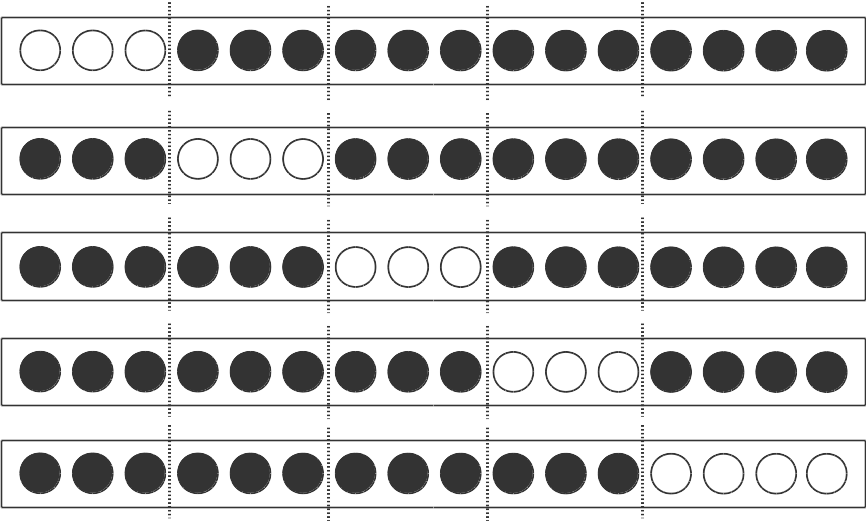
\includegraphics[width=0.5\textwidth]{figures/generalisation/crossval}
  \caption{Une validation crois�e en 5 {\it folds} : Chaque observation
    appartient � un des 5 jeux de validation (en blanc) et aux 4 autres jeux
    d'entra�nement (en noir).}
  \label{fig:crossval}
\end{figure}

\section{Crit�res de performance}
\todo{R��crire de mani�re moins exhaustive ; lien avec erreurs de premi�re et deuxi�me esp�ce d'un test}.

% Il existe de nombreuses fa�ons d'�valuer la performance pr�dictive d'un mod�le
% d'apprentissage supervis�. Cette section pr�sente les principaux crit�res
% utilis�s.

\subsection{Matrice de confusion et crit�res d�riv�s}
\label{sec:confusion_matrix}
Comme nous l'avons vu, le nombre d'erreurs de classification permet d'�valuer
la qualit� d'un mod�le pr�dictif. Notons que l'on pr�f�rera g�n�ralement
d�crire le nombre d'erreurs comme une fraction du nombre d'exemples : un taux
d'erreur de $1\%$ est plus parlant qu'un nombre absolu d'erreurs.
 
Mais toutes les erreurs ne se valent pas n�cessairement. Prenons l'exemple d'un
mod�le qui pr�dise si oui ou non une radiographie pr�sente une tumeur
inqui�tante : une fausse alerte, qui sera ensuite infirm�e par des examens
compl�mentaires, est moins probl�matique que de ne pas d�celer la tumeur et de
ne pas traiter la personne concern�e.  Les performances d'un mod�le de
classification, binaire comme multi-classe, peuvent �tre r�sum�e dans une {\it
  matrice de confusion}.

�tant donn� un probl�me de classification, on appelle {\it matrice de
  confusion} une matrice $M$ contenant autant de lignes que de colonnes que de
classes, et dont l'entr�e $M_{ck}$ est le nombre d'exemples de la classe $c$
pour laquelle l'�tiquette $k$ a �t� pr�dite.

Dans le cas de la classification binaire, la matrice de confusion prend la
forme suivante :
\begin{center}
  \begin{tabular}[h]{|c|c|c|c|} \hline \multicolumn{2}{|c|}{} &
      \multicolumn{2}{|c|}{Classe r�elle} \\ \hline \multicolumn{2}{|c|}{} & 0 & 1 \\ \hline 
    Classe & 0 & vrais n�gatifs (TN) & faux n�gatifs (FN)
    \\ \cline{2-4} pr�dite & 1 & faux positifs (FP) & vrais positifs (TP)
    \\ \hline
  \end{tabular}
\end{center}

On appelle {\it vrais positifs} (en anglais {\it true positives}) les exemples
positifs correctement classifi�s ; {\it faux positifs} (en anglais {\it false
  positives}) les exemples n�gatifs �tiquet�s positifs par le mod�le ; et
r�ciproquement pour les {\it vrais n�gatifs} ({\it true negatives}) et les {\it
  faux n�gatifs} ({\it false negatives}). On note g�n�ralement par {\it TP} le
nombre de vrais positifs, {\it FP} le nombre de faux positifs, {\it TN} le
nombre de vrais n�gatifs et {\it FN} le nombre de faux n�gatifs.

Les faux positifs sont aussi appel�s {\it fausses alarmes} ou {\it erreurs de
  type I}, par opposition aux {\it erreurs de type II} qui sont les faux
n�gatifs.

Il est possible de d�river de nombreux crit�res d'�valuation � partir de la
matrice de confusion. En voici quelques exemples :

On appelle {\it rappel} ({\it recall} en anglais), ou {\it sensibilit�} ({\it
  sensitivity} en anglais), le taux de vrais positifs, c'est-�-dire la
proportion d'exemples positifs correctement identifi�s comme tels :
\begin{equation*}
  \text{Rappel} = \frac{\text{TP}}{\text{TP} + \text{FN}}.
\end{equation*}

Il est cependant tr�s facile d'avoir un bon rappel en pr�disant que {\it tous}
les exemples sont positifs. Ainsi, ce crit�re ne peut pas �tre utilis� seul. On
lui adjoint ainsi souvent la {\it pr�cision} :

On appelle {\it pr�cision}, ou {\it valeur positive pr�dictive} ({\it positive
  predictive value, PPV}) la proportion de pr�dictions correctes parmi les
pr�dictions positives :
\begin{equation*}
  \text{Pr�cision} = \frac{\text{TP}}{\text{TP} + \text{FP}}.
\end{equation*}

De m�me que l'on peut facilement avoir un tr�s bon rappel au d�triment de la
pr�cision, il est ais� d'obtenir une bonne pr�cision (au d�triment du rappel)
en faisant tr�s peu de pr�dictions positives (ce qui r�duit le risque qu'elles
soient erron�es)

L'anglais distingue {\it precision} (la pr�cision ci-dessus) et {\it accuracy},
qui est la proportion d'exemples correctement �tiquet�s, soit le compl�mentaire
� 1 du taux d'erreur, aussi traduit par {\it pr�cision} en fran�ais. On
utilisera donc ces termes avec pr�caution.

Pour r�sumer rappel et pr�cision en un seul nombre, on calculera la {\it
  F-mesure} : \\
On appelle {\it F-mesure} ({\it F-score} ou {\it F1-score} en anglais) la
moyenne harmonique de la pr�cision et du rappel :
\begin{equation*}
  F = 2 \frac{\text{Pr�cision . Rappel}}{\text{Pr�cision} + \text{Rappel}} = 
  \frac{2 \text{TP}}{2 \text{TP} + \text{FP} + \text{FN}}.
\end{equation*}

On appelle {\it sp�cificit�} le taux de vrais n�gatifs, autrement dit la
proportion d'exemples n�gatifs correctement identifi�s comme tels.
\begin{equation*}
  \text{Sp�cificit�} = \frac{\text{TN}}{\text{FP} + \text{TN}}.
\end{equation*}

\subsection{�valuation de m�thodes de classification binaire retournant un
  score}
De nombreux algorithmes de classification ne retournent pas directement une
�tiquette de classe, mais utilisent une fonction de d�cision qui doit ensuite
�tre seuill�e pour devenir une �tiquette. Cette fonction de d�cision peut �tre
un score arbitraire, ou la probabilit� d'appartenir � la classe positive.
  
Plusieurs crit�res permettent d'�valuer la qualit� de la fonction de d�cision
avant seuillage.
  
\subsubsection{Courbe ROC}
On appelle {\it courbe ROC}, de l'anglais {\it Receiver-Operator
  Characteristic} la courbe d�crivant l'�volution de la sensibilit� en fonction
du compl�mentaire � 1 de la sp�cificit�, parfois appel� {\it antisp�cificit�},
lorsque le seuil de d�cision change.

Le terme vient des t�l�communications, o� ces courbes servent � �tudier si un
syst�me arrive � s�parer le signal du bruit de fond.

On peut synth�tiser une courbe ROC par l'aire sous cette courbe, souvent
abr�g�e {\it AUROC} pour {\it Area Under the ROC}.

Un exemple de courbe ROC est pr�sent� sur la figure~\ref{fig:roc_curve}. Le
point $(0, 0)$ appara�t quand on utilise comme seuil un nombre sup�rieur � la
plus grande valeur retourn�e par la fonction de d�cision : ainsi, tous les
exemples sont �tiquet�s n�gatifs. � l'inverse, le point $(1, 1)$ appara�t quand
on utilise pour seuil une valeur inf�rieure au plus petit score retourn� par la
fonction de d�cision : tous les exemples sont alors �tiquet�s positifs.

\begin{figure}[h]
  \centering
  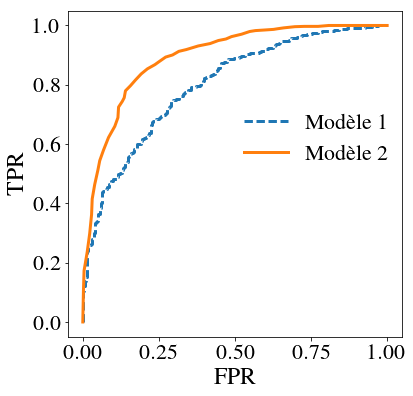
\includegraphics[width=0.5\textwidth]{figures/generalisation/roc_curve}
  \caption{Les courbes ROC de deux mod�les.}
  \label{fig:roc_curve}
\end{figure}

Pour construire la courbe ROC, on prend pour seuil les valeurs successives de
la fonction de d�cision sur notre jeu de donn�es. Ainsi, � chaque nouvelle
valeur de seuil, une observation que l'on pr�disait pr�c�demment n�gative
change d'�tiquette. Si cette observation est effectivement positive, la
sensibilit� augmente de $1/n_p$ (o� $n_p$ est le nombre d'exemples positifs) ;
sinon, c'est l'antisp�cificit� qui augmente de $1/n_n$, o� $n_n$ est le nombre
d'exemples n�gatifs. La courbe ROC est donc une courbe en escaliers.

Un classifieur id�al, qui ne commet aucune erreur, associe syst�matique des
scores plus faibles aux exemples n�gatifs qu'aux exemples positifs. Sa courbe
ROC suit donc le coin sup�rieur gauche du carr� $[0, 1]^2$ ; il a une aire sous
la courbe de 1.

La courbe ROC d'un classifieur al�atoire, qui fera sensiblement la m�me
proportion d'erreurs que de classifications correctes quel que soit le seuil
utilis�, suit la diagonale de ce carr�. L'aire sous la courbe ROC d'un
classifieur al�atoire vaut donc 0.5.

On peut enfin utiliser la courbe ROC pour choisir un seuil de d�cision, �
partir de la sensibilit� (ou de la sp�cificit�) que l'on souhaite garantir.

\subsection{Erreurs de r�gression}
Dans le cas d'un probl�me de r�gression, le nombre d'erreurs n'est pas un
crit�re appropri� pour �valuer la performance. D'une part, � cause des
impr�cisions num�riques, il est d�licat de dire d'une pr�diction � valeur
r�elle si elle est correcte ou non. D'autre part, un mod�le dont $50\%$ des
pr�dictions sont correctes � $0.1\%$ pr�s et les $50$ autres pourcent sont tr�s
�loign�es des vraies valeurs vaut-il mieux qu'un mod�le qui n'est correct qu'�
$1\%$ pr�s, mais pour $100\%$ des exemples ?

Ainsi, on pr�f�rera quantifier la performance d'un mod�le de r�gression en
fonction de l'�cart entre les pr�dictions et les valeurs r�elles.

Un premier crit�re est donc l'erreur quadratique moyenne : \\
�tant donn�es $n$ �tiquettes r�elles $y^1, y^2, \dots, y^n$ et $n$ pr�dictions
$f(\xx^1), f(\xx^2), \dots, f(\xx^n)$, on appelle {\it erreur quadratique
  moyenne}, ou {\it MSE} de l'anglais {\it mean squared error} la valeur
\begin{equation*}
  \text{MSE} = \frac1n \sum_{i=1}^n \left( f(\xx^i) - y^i \right)^2.
\end{equation*}

Pour mesurer l'erreur dans la m�me unit� que la cible, on lui pr�f�re souvent
sa racine : \\
�tant donn�es $n$ �tiquettes r�elles $y^1, y^2, \dots, y^n$ et $n$ pr�dictions
$f(\xx^1), f(\xx^2), \dots, f(\xx^n)$, on appelle {\it racine de l'erreur
  quadratique moyenne}, ou {\it RMSE} de l'anglais {\it root mean squared
  error} la valeur
\begin{equation*}
  \text{RMSE} = \sqrt{\frac1n \sum_{i=1}^n \left( f(\xx^i) - y^i \right)^2}.
\end{equation*}

L'interpr�tation de ces erreurs requiert n�anmoins de conna�tre la distribution
des valeurs cibles : une RMSE de 1 cm n'aura pas la m�me signification selon
qu'on essaie de pr�dire la taille d'humains ou celle de drosophiles.  Pour
r�pondre � cela, il est possible de normaliser la somme des carr�s des r�sidus
non pas en en faisant la moyenne, mais en la comparant � la somme des distances
des valeurs cibles � leur moyenne.  �tant donn�es $n$ �tiquettes r�elles
$y^1, y^2, \dots, y^n$ et $n$ pr�dictions
$f(\xx^1), f(\xx^2), \dots, f(\xx^n)$, on appelle {\it erreur carr�e relative},
ou {\it RSE} de l'anglais {\it relative squared error} la valeur
\begin{equation*}
  \text{RSE} = \frac{ \sum_{i=1}^n \left( f(\xx^i) - y^i \right)^2}{
    \sum_{i=1}^n \left( y^i - \frac1n \sum_{l=1}^n y^l \right)^2}.
\end{equation*}

Le compl�mentaire � 1 de la RSE est le {\it coefficient de d�termination}, not�
$R^2$.

On note le coefficient de d�termination $R^2$ car il s'agit du carr� du
coefficient de corr�lation entre $\yy$ et
$(f(\xx^1), f(\xx^2), \dots, f(\xx^n))$ donn� par
\begin{equation}
  \label{eq:pearson}
  R = \frac{\sum_{i=1}^n \left( y^i -  \frac1n \sum_{l=1}^n y^l \right)
    \left( f(\xx^i) -  \frac1n \sum_{i=1}^n f(\xx^i) \right)}{
    \sqrt{\sum_{i=1}^n \left( y^i -  \frac1n \sum_{l=1}^n y^l \right)^2}
    \sqrt{\sum_{i=1}^n \left( f(\xx^i) -  \frac1n \sum_{l=1}^n f(\xx^l) \right)^2}.
  }
\end{equation}
Ce coefficient indique � quel point les valeurs pr�dites sont corr�l�es aux
valeurs r�elles ; attention, il sera �lev� aussi si elles leur sont
anti-corr�l�es.

\section{R�gularisation}
\label{sec:generalization_regularization}
Plus un mod�le est simple, et moins il a de chances de sur-apprendre. Pour
limiter le risque de sur-apprentissage, il est donc souhaitable de limiter la
complexit� d'un mod�le. C'est ce que permet de faire la {\it r�gularisation},
une technique qui consiste � ajouter au terme d'erreur que l'on cherche �
minimiser un terme qui mesure la complexit� du probl�me (par exemple, dans le
cas pr�c�dent, le degr� du polyn�me ou le nombre de coefficients du
mod�le). Ainsi, un mod�le complexe qui a une erreur empirique faible peut �tre
d�favoris� face � une mod�le plus simple, m�me si celui-ci pr�sente une erreur
empirique plus �lev�e.

Lorsque les variables sont fortement corr�l�es, ou que leur nombre d�passe
celui des observations, la matrice $X \in \RR^{p+1}$ repr�sentant nos donn�es
ne peut pas �tre de rang colonne plein. Ainsi, la matrice $X^\top X$ n'est pas
inversible et il n'existe pas de solution unique � une r�gression lin�aire par
minimisation des moindres carr�s. Il y a donc un risque de sur-apprentissage :
le mod�le n'�tant pas unique, comment peut-on garantir que c'est celui que l'on
a s�lectionn� qui g�n�ralise le mieux ?

Pour limiter ce risque de sur-apprentissage, nous allons chercher � contr�ler
simultan�ment l'erreur du mod�le sur le jeu d'entra�nement et les valeurs des
coefficients de r�gression affect�s � chacune des variables. Contr�ler ces
coefficients est une fa�on de contr�ler la complexit� du mod�le : comme nous le
verrons par la suite, ce contr�le consiste � contraindre les coefficients �
appartenir � un sous-ensemble strict de $\RR^{p+1}$ plut�t que de pouvoir
prendre n'importe quelle valeur dans cet espace, ce qui restreint l'espace des
solutions possibles.

On appelle {\it r�gularisation} le fait d'apprendre un mod�le en minimisant la
somme du risque empirique sur le jeu d'entra�nement et d'un terme de contrainte
$\Omega$ sur les solutions possibles :
\begin{equation}
  \label{eq:regularisation}
  f = \argmin_{h \in \FF} \frac{1}{n} \sum_{i=1}^n L(h(\xx^i), y^i) + 
  \lambda \Omega(h),
\end{equation}
o� le coefficient de r�gularisation $\lambda \in \RR_+$ contr�le
l'importance relative de chacun des termes.
 
Dans le cas d'un mod�le de r�gression lin�aire, nous allons utiliser comme
fonction de perte la somme des moindres carr�s. Les r�gulariseurs que nous
allons voir sont fonction du vecteur de coefficients de r�gression $\bbeta$ :
\begin{equation*}
  \argmin_{\bbeta \in \RR^{p+1}} \left(\yy - X \bbeta \right)^\top 
  \left(\yy - X \bbeta \right) + \lambda \Omega(\bbeta)
\end{equation*}
ou, de mani�re �quivalente, 
\begin{equation}
  \label{eq:regularisation_linreg}
  \argmin_{\bbeta \in \RR^{p+1}} \ltwonorm{\yy - X \bbeta}^2 + \lambda \Omega(\bbeta).
\end{equation}
Nous utilisons ici la transformation~\ref{eq:added_ones} de $\xx$ qui
consiste � ajouter � la matrice de design $X$ une colonne de 1 pour
simplifier les notations.

Le coefficient de r�gularisation $\lambda$ est un hyperparam�tre de la
r�gression lin�aire r�gularis�e.

Quand $\lambda$ tend vers $+\infty$, le terme de r�gularisation prend de plus
en plus d'importance, jusqu'� ce qu'il domine le terme d'erreur et que seule
compte la minimisation du r�gulariseur. Dans la plupart des cas, le
r�gulariseur est minimis� quand $\bbeta = \vec{0}$, et il n'y a plus
d'apprentissage.
  
� l'inverse, quand $\lambda$ tend vers $0$, le terme de r�gularisation devient
n�gligeable devant le terme d'erreur, et $\bbeta$ prendra comme valeur une
solution de la r�gression lin�aire non r�gularis�e.

Comme tout hyperparam�tre, $\lambda$ peut �tre choisi par validation
crois�e. On utilisera g�n�ralement une grille de valeurs logarithmique.

\section{La r�gression ridge}
\label{sec:ridge_regression}
Une des formes les plus courantes de r�gularisation, utilis�e dans de
nombreux domaines faisant intervenir des probl�mes inverses mal pos�s,
consiste � utiliser comme r�gulariseur la norme $\ell_2$ du vecteur 
$\bbeta$ :  
\begin{equation}
  \label{eq:l2norm_reg}
  \Omega_{\text{ridge}}(\bbeta) = \ltwonorm{\bbeta}^2 = \sum_{j=0}^p \beta_j^2.
\end{equation}

\subsection{Formulation de la r�gression ridge}
On appelle {\it r�gression ridge} le mod�le $f: x \mapsto \bbeta^\top \xx$ dont
les coefficients sont obtenus par
\begin{equation}
  \label{eq:ridgereg}
  \argmin_{\bbeta \in \RR^{p+1}} \ltwonorm{\yy - X \bbeta}^2 + 
  \lambda \ltwonorm{\bbeta}^2.
\end{equation}    

% La r�gression ridge est un cas particulier de {\it r�gularisation de Tikhonov}
% (d�velopp�e pour r�soudre des �quations int�grales).  Elle intervient aussi
% dans les r�seaux de neurones, o� elle est appel�e {\it weight decay}
% (d�gradation / mod�ration des pond�rations, voir section~\ref{sec:saturation}).

\subsection{Solution}
Le probl�me~\ref{eq:ridgereg} est un probl�me d'optimisation convexe : il s'agit de minimiser une forme
quadratique. Il se r�sout en annulant le gradient en $\bbeta$ de la fonction
objective :
\begin{equation}
  \nabla_{\bbeta} \left( \ltwonorm{\yy - X \bbeta}^2 + 
    \lambda \ltwonorm{\bbeta}^2 \right) = 0
\end{equation}

En notant $I_p \in \RR^{p \times p}$ la matrice identit� en dimension $p,$ on
obtient :
\begin{equation}
  \left( \lambda I_p + X^\top X  \right) \bbeta^* = X^\top \yy.
\end{equation}
Comme $\lambda > 0$, la matrice $\lambda I_p + X^\top X$ est toujours
inversible. Notre probl�me admet donc toujours une unique solution
explicite. La r�gularisation par la norme $\ell_2$ a permis de transformer un
probl�me potentiellement mal pos� en un probl�me bien pos�, dont la solution
est :
\begin{equation}
  \label{eq:ridgereg_sol}
  \bbeta^* =  \left( \lambda I_p + X^\top X  \right)^{-1} X^\top \yy.
\end{equation}
  
Si l'on multiplie la variable $x_j$ par une constante $\alpha$, le coefficient
correspondant dans la r�gression lin�aire non r�gularis�e est divis� par
$\alpha.$ En effet, si on appelle $X^*$ la matrice obtenue en rempla�ant $x_j$
par $\alpha x_j$ dans $X$, la solution $\bbeta^*$ de la r�gression lin�aire
correspondante v�rifie $X^* \left( \yy - X^* \bbeta^* \right) = 0$, tandis que
la solution $\bbeta$ de la r�gression lin�aire sur $X$ v�rifie
$X \left( \yy - X \bbeta \right) = 0.$ Ainsi, changer l'�chelle d'une variable
a comme seul impact sur la r�gression lin�aire non r�gularis�e d'ajuster le
coefficient correspondant de mani�re inversement proportionnelle.

� l'inverse, dans le cas de la r�gression ridge, remplacer $x_j$ par
$\alpha x_j$ affecte aussi le terme de r�gularisation, et a un effet plus
complexe. L'�chelle relative des diff�rentes variables peut donc fortement
affecter la r�gression ridge. Il est ainsi recommand� de {\it standardiser} les
variables avant l'apprentissage, c'est-�-dire de toutes les ramener � avoir un
�cart-type de 1 en les divisant par leur �cart-type :
\begin{equation}
  \label{eq:standardisation}
  x_j^i \leftarrow \frac{x_j^i}{\sqrt{\frac1n \sum_{i=1}^n \left( x_j^i - 
        \frac1n \sum_{i=1}^n x_j^i \right)^2}}
\end{equation}    
Attention : pour �viter le sur-apprentissage, il est important que cet
�cart-type soit calcul� sur le jeu d'entra�nement uniquement, puis appliqu�
ensuite aux jeux de test ou validation.

La r�gression ridge a un effet de \og regroupement \fg~sur les variables
corr�l�es, au sens o� des variables corr�l�es auront des coefficients
similaires.

\subsection{Chemin de r�gularisation}
On appelle {\it chemin de r�gularisation} l'�volution de la valeur du
coefficient de r�gression d'une variable en fonction du coefficient de
r�gularisation $\lambda$.

Le chemin de r�gularisation permet de comprendre l'effet de la r�gularisation
sur les valeurs de $\bbeta$. En voici un exemple sur la
figure~\ref{fig:ridge_path}.

\begin{figure}[h]
  \centering
  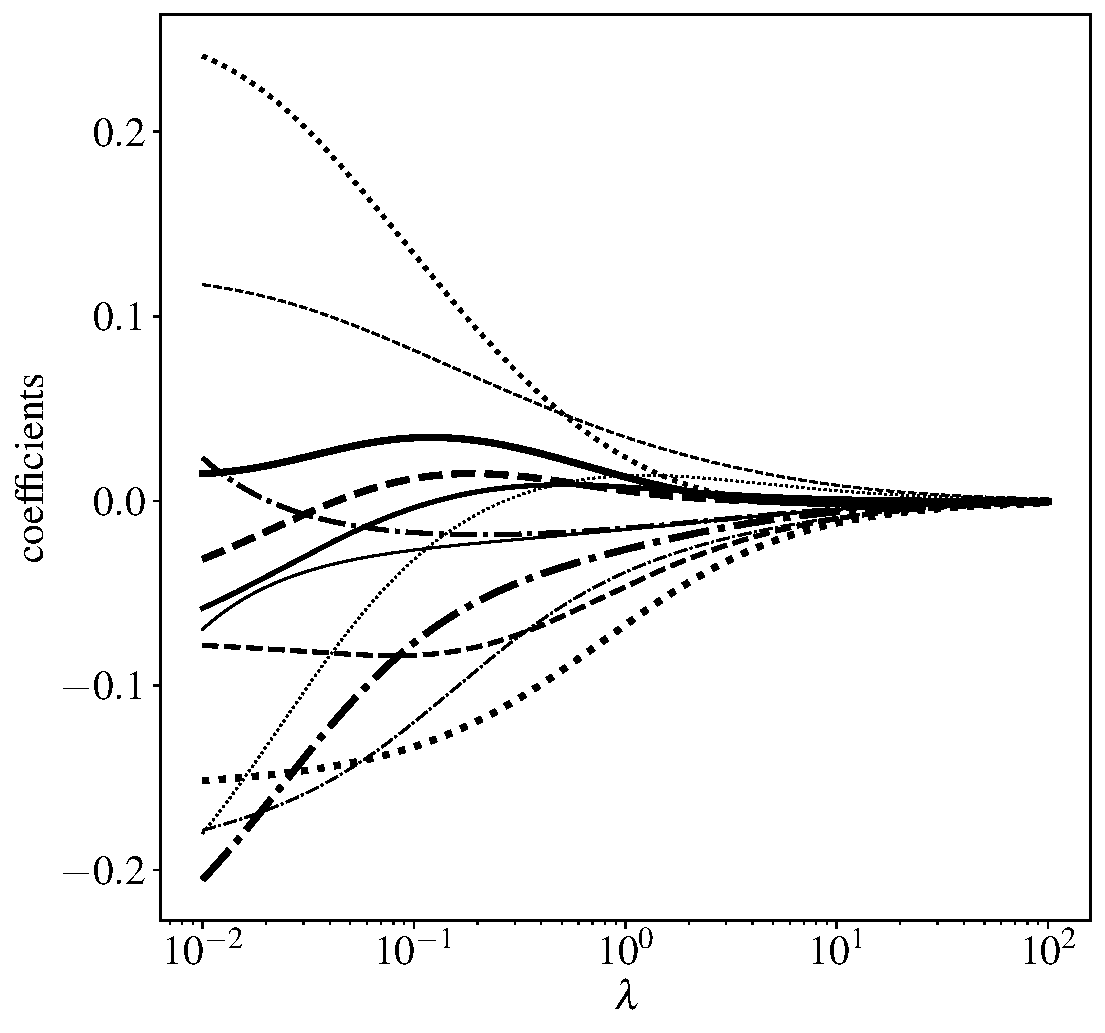
\includegraphics[width=0.5\textwidth]{figures/generalisation/ridge_path}
  \caption{Chemin de r�gularisation de la r�gression ridge pour un jeu de
    donn�es avec 12 variables. Chaque ligne repr�sente l'�volution du
    coefficient de r�gression d'une de ces variables quand $\lambda$ augmente :
    le coefficient �volue de sa valeur dans la r�gression non r�gularis�e vers
    0.}
  \label{fig:ridge_path}
\end{figure}

\subsection{Interpr�tation g�om�trique}
�tant donn�s $\lambda \in \RR_+$, $X \in \RR^{n \times p}$ et $\yy \in \RR^n$,
il existe un unique $t \in \RR_+$ tel que le probl�me~\ref{eq:ridgereg} soit
�quivalent �
\begin{equation}
  \label{eq:ridgereg_dual}
  \argmin_{\bbeta \in \RR^{p+1}} \ltwonorm{\yy - X \bbeta}^2 \text{ tel que }
  \ltwonorm{\bbeta}^2 \leq t.
\end{equation}
Preuve : L'�quivalence s'obtient par dualit� et en �crivant les conditions de
Karun-Kush-Tucker.
  
La r�gression ridge peut donc �tre formul�e comme un probl�me d'optimisation
quadratique (minimiser $\ltwonorm{\yy - X \bbeta}^2$) sous contraintes
($\ltwonorm{\bbeta}^2 \leq t$) : la solution doit �tre contenue dans la boule
$\ell_2$ de rayon $\sqrt{t}$. Sauf dans le cas o� l'optimisation sans
contrainte v�rifie d�j� la condition, cette solution sera sur la fronti�re de
cette boule, comme illustr� sur la figure~\ref{fig:l2reg}.

\begin{figure}[h]
  \centering
  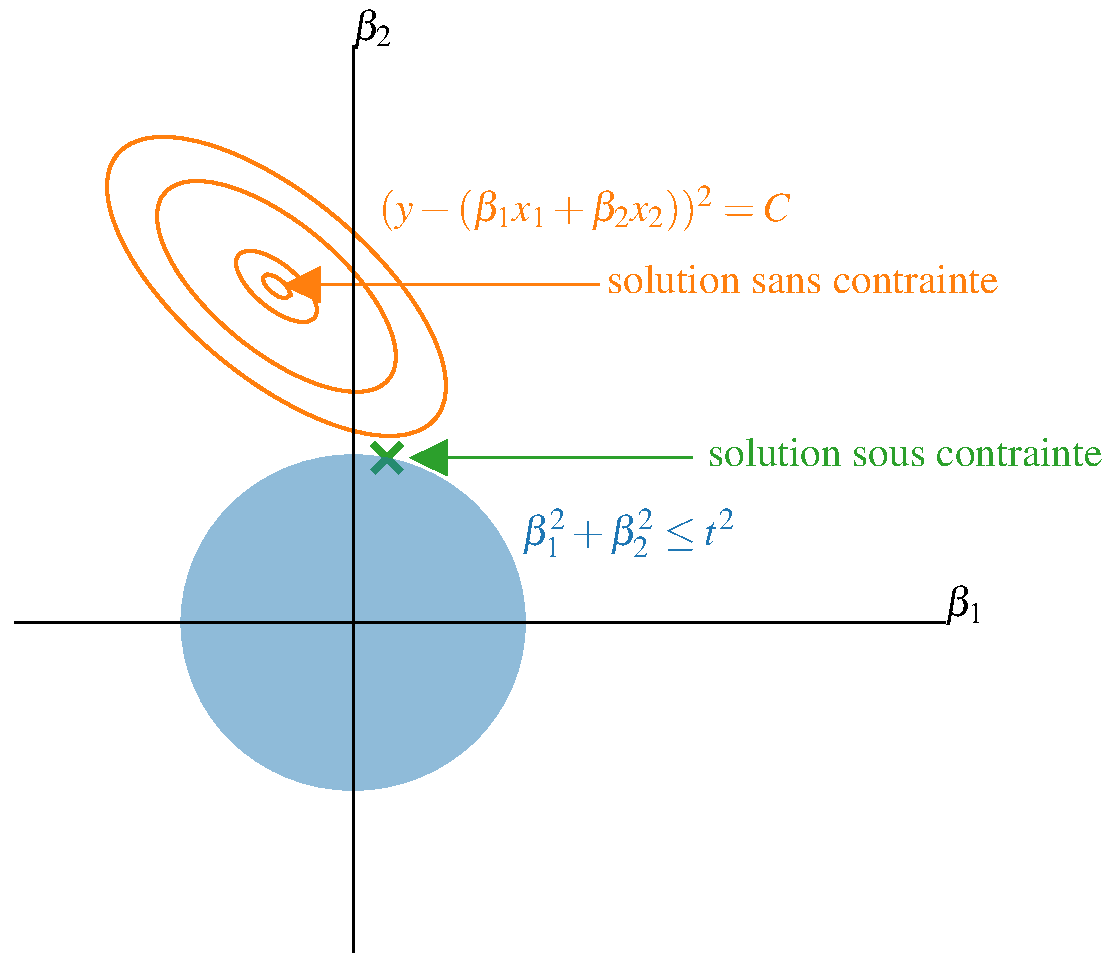
\includegraphics[width=0.7\textwidth]{figures/generalisation/l2reg}
  \caption{La solution du probl�me d'optimisation sous
    contraintes~\ref{eq:ridgereg_dual} (ici en deux dimensions) se situe sur
    une ligne de niveau de la somme des moindres carr�s tangente � la boule
    $\ell_2$ de rayon $\sqrt{t}$.}
  \label{fig:l2reg}
\end{figure}
  
\section{Le lasso}
\label{sec:lasso}

\subsection{Parcimonie}
Dans certaines applications, il peut �tre raisonnable de supposer que
l'�tiquette que l'on cherche � pr�dire n'est expliqu�e que par un nombre
restreint de variables. Il est dans ce cas souhaitable d'avoir un mod�le {\it
  parcimonieux}, ou {\it sparse}, c'est-�-dire dans lequel un certain nombre de
coefficients sont nuls : les variables correspondantes peuvent �tre retir�es du
mod�le.

Pour ce faire, Robert Tibshirani a propos� en 1996 d'utiliser comme
r�gulariseur la norme $\ell_1$ du coefficient $\bbeta$ :
\begin{equation}
  \label{eq:l1norm_reg}
  \Omega_{\text{lasso}}(\bbeta) = \lonenorm{\bbeta} = \sum_{j=0}^p \lvert \beta_j \rvert.
\end{equation}

Pour comprendre pourquoi ce r�gulariseur permet de \og pousser \fg~certains
coefficients vers 0, on se reportera � la section~\ref{sec:interp_geom_lasso}
et � la figure~\ref{fig:l1reg}.

\subsection{Formulation du lasso}
On appelle {\it lasso} le mod�le $f: x \mapsto \bbeta^\top \xx$ dont les
coefficients sont obtenus par
\begin{equation}
  \label{eq:lasso}
  \argmin_{\bbeta \in \RR^{p+1}} \ltwonorm{\yy - X \bbeta}^2 + 
  \lambda \lonenorm{\bbeta}.
\end{equation}    
Le nom de lasso est en fait un acronyme, pour {\it Least Absolute Shrinkage and
  Selection Operator} : il s'agit d'une m�thode qui utilise les valeurs {\it
  absolues} des coefficients (la norme $\ell_1$) pour r�duire ({\it shrink})
ces coefficients, ce qui permet de {\it s�lectionner} les variables qui
n'auront pas un coefficient nul. En traitement du signal, le lasso est aussi
connu sous le nom de {\it poursuite de base} ({\it basis pursuit} en anglais).

En cr�ant un mod�le parcimonieux et en permettant d'�liminer les variables
ayant un coefficient nul, le lasso est une m�thode de s�lection de variables
supervis�e. Il s'agit donc aussi d'une m�thode de r�duction de dimension.

\subsection{Solution}
Le lasso~\ref{eq:lasso} n'admet pas de solution explicite. On pourra utiliser
un algorithme � directions de descente  pour le r�soudre. De plus, il ne s'agit pas
toujours d'un probl�me strictement convexe (en particulier, quand $p > n$) et
il n'admet donc pas n�cessairement une unique solution. En pratique, cela pose
surtout probl�me quand les variables ne peuvent pas �tre consid�r�es comme les
r�alisations de lois de probabilit� continues.
N�anmoins, % s'il est possible que plusieurs $\bbeta$ minimisent la
  % fonction objective du lasso, leur produit � gauche par $X$ vaut toujours la
  % m�me valeur (par convexit� stricte de la fonction de co�t) ; cela permet de
  % montrer que 
il est possible de montrer que les coefficients non nuls dans deux solutions
ont n�cessairement le m�me signe. Ainsi, l'effet d'une variable a la m�me
direction dans toutes les solutions qui la consid�rent, ce qui facilite
l'interpr�tation d'un mod�le appris par le lasso.
  
\subsection{Interpr�tation g�om�trique}
\label{sec:interp_geom_lasso}
Comme pr�c�demment, le probl�me~\ref{eq:lasso} peut �tre reformul� comme un
probl�me d'optimisation quadratique sous contraintes :

�tant donn�s $\lambda \in \RR_+$, $X \in \RR^{n \times p}$ et $\yy \in \RR^n$,
il existe un unique $t \in \RR_+$ tel que le probl�me~\ref{eq:lasso} soit
�quivalent �
\begin{equation}
  \label{eq:lasso_dual}
  \argmin_{\bbeta \in \RR^{p+1}} \ltwonorm{\yy - X \bbeta}^2 \text{ tel que }
  \lonenorm{\bbeta} \leq t.
\end{equation}

La solution doit maintenant �tre contenue dans la boule $\ell_1$ de rayon
$t$. Comme cette boule a des \og coins \fg, les lignes de niveau de la forme
quadratique sont plus susceptibles d'y �tre tangente en un point o� une ou
plusieurs coordonn�es sont nulles (voir figure~\ref{fig:l1reg}).

\begin{figure}[h]
  \centering 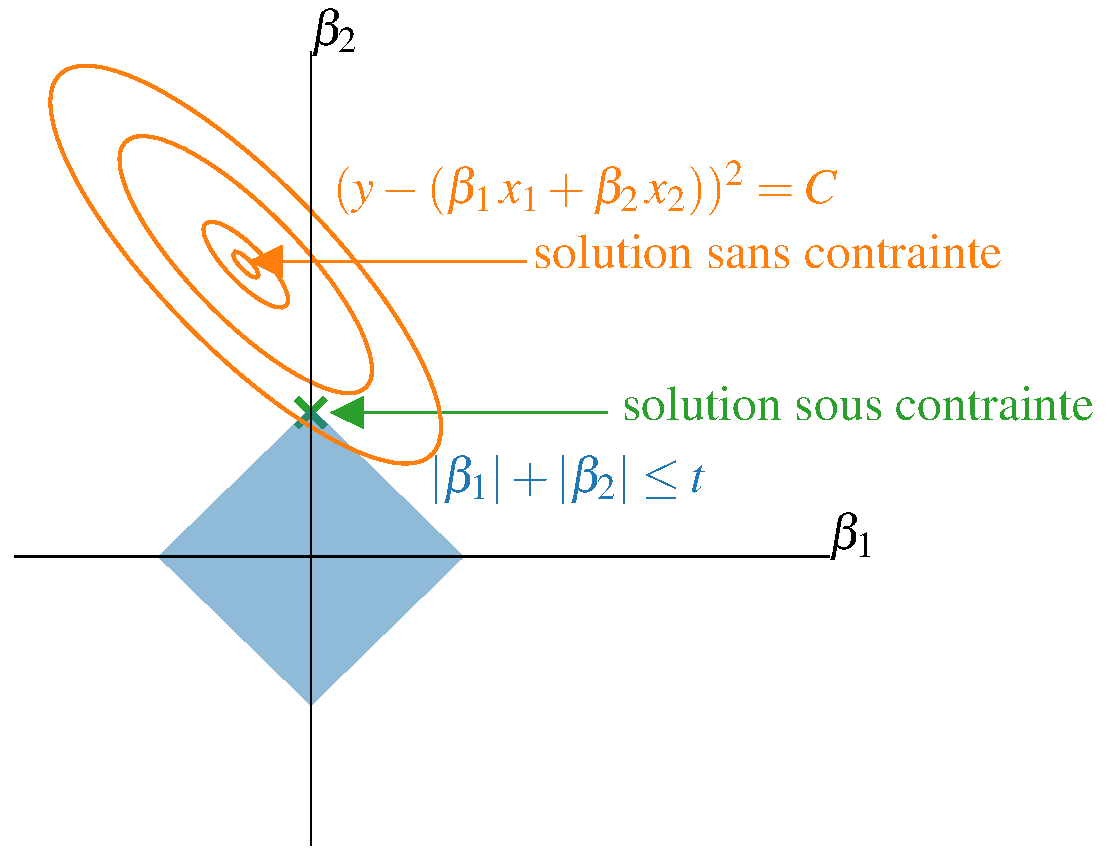
\includegraphics[width=0.5\textwidth]{figures/generalisation/l1reg}
  \caption{La solution du probl�me d'optimisation sous
    contraintes~\ref{eq:lasso_dual} (ici en deux dimensions) se situe sur
    une ligne de niveau de la somme des moindres carr�s tangente � la boule
    $\ell_1$ de rayon $t$.}
  \label{fig:l1reg}
\end{figure}


\subsection{Chemin de r�gularisation}
Sur le chemin de r�gularisation du lasso (par exemple
figure~\ref{fig:lasso_path}, sur les m�mes donn�es que pour la
figure~\ref{fig:ridge_path}), on observe que les variables sortent du mod�le
les unes apr�s les autres, jusqu'� ce que tous les coefficients soient nuls. On
remarquera aussi que le chemin de r�gularisation pour n'importe quelle variable
est lin�aire par morceaux ; c'est une propri�t� du lasso.
\begin{figure}[h]
  \centering
  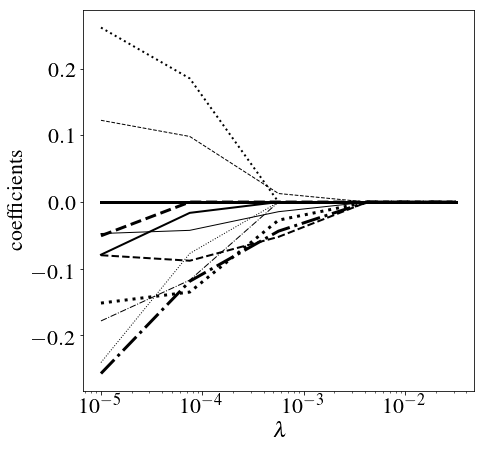
\includegraphics[width=0.5\textwidth]{figures/generalisation/lasso_path}
  \caption{Chemin de r�gularisation du lasso pour un jeu de donn�es avec 12
    variables. Chaque ligne repr�sente l'�volution du coefficient de r�gression
    d'une de ces variables quand $\lambda$ augmente : les variables sont
    �limin�es les unes apr�s les autres.}
  \label{fig:lasso_path}
\end{figure}

Si plusieurs variables corr�l�es contribuent � la pr�diction de l'�tiquette, le
lasso va avoir tendance � choisir une seule d'entre elles (affectant un poids
de 0 aux autres), plut�t que de r�partir les poids �quitablement comme la
r�gression ridge. C'est ainsi qu'on arrive � avoir des mod�les tr�s
parcimonieux. Cependant, le choix de cette variable est al�atoire, et peut
changer si l'on r�p�te la proc�dure d'optimisation. Le lasso a donc tendance �
�tre instable.

\section{Exercice : SVM lin�aire pour la r�gression}
\todo{}

% \section{Points cl�s}
% \begin{itemize}
% \item Le compromis biais-variance traduit le compromis entre l'erreur
%   d'approximation, correspondant au biais de l'algorithme d'apprentissage, et
%   l'erreur d'estimation, correspondant � sa variance.
% \item La g�n�ralisation et le sur-apprentissage sont des pr�occupations
%   majeures en machine learning : comment s'assurer que des mod�les entra�n�s
%   pour minimiser leur erreur de pr�diction sur les donn�es observ�es seront
%   g�n�ralisables aux donn�es pour lesquelles il nous int�resse de faire des
%   pr�dictions ?
% \item Ajouter un terme de r�gularisation, fonction du vecteur des coefficients
%   $\bbeta$, au risque empirique de la r�gression lin�aire permet d'�viter le
%   sur-apprentissage
% \item La r�gression ridge utilise la norme $\ell_2$ de $\bbeta$ comme
%   r�gulariseur ; elle admet toujours une unique solution analytique, et a un
%   effet de regroupement sur les variables corr�l�es.
% \item Le lasso utilise la norme $\ell_1$ de $\bbeta$ comme r�gulariseur ; il
%   cr�e un mod�le parcimonieux, et permet donc d'effectuer une r�duction de
%   dimension supervis�e.
% \end{itemize}


%%% Local Variables:
%%% mode: latex
%%% TeX-master: "sdd_2020_poly"
%%% End:
% \clearpage 

% \chapter{Mod�les non-lin�aires}
% %-*- coding: iso-latin-1 -*-
\label{chap:nonlin}


\paragraph{Notions :} r�seaux de neurones artificiels, apprentissage profond,
arbres de d�cision et for�ts al�atoires, m�thodes � noyaux.
\paragraph{Objectifs p�dagogiques :} 
\begin{itemize}      
  \setlength{\itemsep}{3pt}
\item D�crire les similarit�s et diff�rences entre r�seaux de neurones artificiels et mod�les lin�aires ; 
\item Utiliser l'astuce du noyau pour apprendre des mod�les non-lin�aires �
  partir des algorithmes lin�aires vus pr�c�demment ;
\item Mettre en \oe{}uvre un algorithme d'apprentissage ensembliste.
\end{itemize}

Tous les mod�les d'apprentissage supervis� que nous avons vus jusqu'� pr�sent
utilisent une fonction lin�aire des variables. Il s'agit dans ce chapitre
d'aborder comment construire des mod�les non-lin�aires, dont la capacit� de
mod�lisation sup�rieure pourra permettre d'apprendre des mod�les plus complexes. Attention n�anmoins au surapprentissage !

Dans ce chapitre, nous consid�rons sauf mention contraire un jeu de donn�es
$\DD = \{\xx^i, y^i\}_{i=1, \dots, n}$ de $n$ observations en $p$ dimensions et
leurs �tiquettes dans $\YY$, avec $\YY= \{0, 1\}$ pour un probl�me de
classification binaire et $\YY = \RR$ pour un probl�me de r�gression.

\section{Mod�les param�triques non-lin�aires}

\subsection{R�gression polynomiale}
\label{sec:polynomial_reg}
Une premi�re fa�on de construire des mod�les non-lin�aires, que nous avons
bri�vement abord�e dans la PC~5, consiste � apprendre une fonction de
d�cision de la forme suivante :
\begin{equation}
  \label{eq:polynomial_decision}
  f: \xx \mapsto \beta^0_0 + \sum_{j=1}^p \beta^1_{j} x_j + 
  \sum_{j=1}^p \sum_{k=1}^p \beta^2_{jk} x_j x_k + \dots +
  \underbrace{\sum_{j=1}^p \dots \sum_{\xi=1}^p}_{d \text{ termes}} \beta^d_{jk\dots\xi} x_j x_k \dots x_{\xi}.
\end{equation}
On parle alors de \textbf{r�gression polynomiale} de degr� $d$.

Il s'agit en fait simplement d'une r�gression lin�aire sur ${d+p \choose p}$ variables.

Attention, on cr�e ainsi un grand nombre de variables, corr�l�es entre elles :
il est alors indispensable d'utiliser un terme de r�gularisation pour �viter le
surapprentissage.

Le principe s'applique aussi � la r�gression logistique (vue dans la PC~6).


\subsection{Perceptron}
Les r�seaux de neurones artificiels permettent d'autres formes de r�gressions
non-lin�aires, et sont bien plus flexibles que les r�gressions polynomiales.


L'histoire des r�seaux de neurones artificiels remonte aux ann�es 1950 et aux
efforts de psychologues comme Franck Rosenblatt pour comprendre le cerveau
humain. Initialement, ils ont �t� con�us dans le but de mod�liser
math�matiquement le traitement de l'information par les r�seaux de neurones
biologiques qui se trouvent dans le cortex des mammif�res. De nos jours, leur
r�alisme biologique importe peu et c'est leur efficacit� � mod�liser des
relations complexes et non lin�aires qui fait leur succ�s.
  
Le premier r�seau de neurones artificiels est le \textbf{perceptron}, propos�
par Rosenblatt en 1957. Il comporte une seule couche et a une capacit� de
mod�lisation limit�e.
Le perceptron (figure~\ref{fig:perceptron}) est form� d'une couche d'entr�e de
$p$ neurones, ou \textbf{unit�s}, correspondant chacune � une variable
d'entr�e. Ces neurones transmettent la valeur de leur entr�e � la couche
suivante.  � ces $p$ neurones on ajoute g�n�ralement une unit� de biais, qui
transmet toujours la valeur $1$. Cette unit� correspond � la colonne de $1$ que
nous avons ajout�e aux donn�es dans les mod�les lin�aires
(�quation~\eqref{eq:added_ones}). On remplacera dans cette section tout vecteur
$\xx = (x_1, x_2, \dots, x_p)$ par sa version augment�e d'un 1 :
$\xx = (1, x_1, x_2, \dots, x_p)$.

La premi�re et unique couche du perceptron (apr�s la couche d'entr�e) contient
un seul neurone, auquel sont connect�es toutes les unit�s de la couche
d'entr�e.

Ce neurone calcule une combinaison lin�aire
$o(\xx) = w_0 + \sum_{j=1}^p w_j x_j$ des signaux $x_1, x_2,  \dots, x_p$
qu'il re�oit en entr�e, auquel il applique une \textbf{fonction d'activation}
$a$, dont il transmet en sortie le r�sultat. Cette sortie met en {\oe}uvre la
fonction de d�cision du perceptron.

Ainsi, si l'on appelle $w_j$ le poids de connexion entre l'unit� d'entr�e $j$
et le neurone de sortie, ce neurone calcule
\begin{equation}
  \label{eq:perceptron_sortie}
  f(\xx) = a(o(\xx)) = a\left(w_0 + \sum_{j=1}^p w_j x_j \right) 
  = a\left(\innerproduct{\ww,~\xx} \right).
\end{equation}
Il s'agit donc bien d'un mod�le param�trique.

\begin{figure}[h]
  \centering
  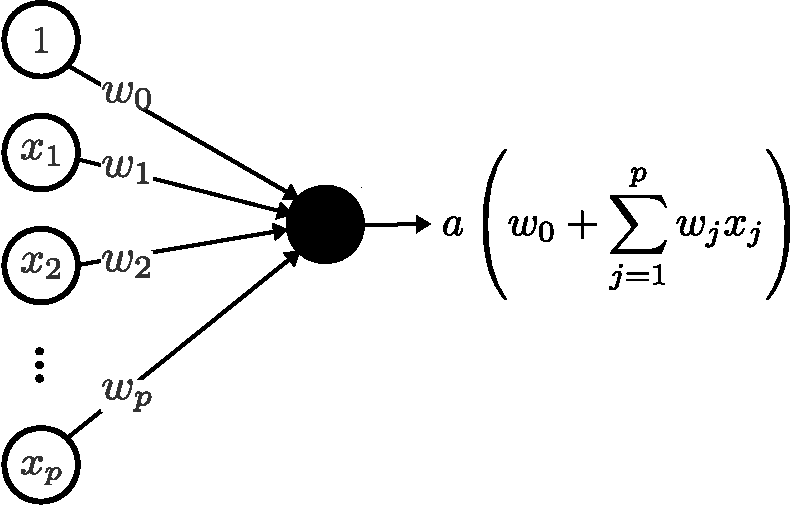
\includegraphics[width=0.5\textwidth]{figures/nonlin/perceptron}
  \caption{Architecture d'un perceptron. }
  \label{fig:perceptron}
\end{figure}

Dans le cas d'un probl�me de r�gression, on utilisera tout simplement l'identit� comme fonction d'activation. Le mod�le appris est donc $\xx \mapsto \innerproduct{\ww, \xx},$ comme dans le cas de la r�gression lin�aire.

Le cas de la classification binaire, utilisant un seuil comme fonction
d'activation, est historiquement le premier � avoir �t� trait�. Ce cas est
d�taill� dans la section~\ref{sec:perceptron_binary}.  On utilisera plut�t,
comme
% \item Pour pr�dire la probabilit� d'appartenir � la classe positive, comme
dans le cas de la r�gression logistique (voir PC~6), une fonction logistique. Le mod�le appris est donc
\begin{equation}
  \xx \mapsto \frac1{1 + e^{- o(\xx)}} = 
  \frac1{1 + \exp \left( - \innerproduct{\ww,~\xx} \right)}.
\end{equation}


\paragraph{Minimisation du risque empirique} Pour entra�ner un perceptron, nous
allons chercher, comme pour toute r�gresssion param�trique, � minimiser le
risque empirique.  Cependant, nous allons supposer que les observations
$(\xx^i, y^i)$ ne sont pas disponibles simultan�ment, mais qu'elles sont
observ�es s�quentiellement. Cette hypoth�se d�coule de la plasticit� des
r�seaux de neurones biologiques : ils s'adaptent constamment en fonction des
signaux qu'ils re�oivent. Nous allons donc utiliser un algorithme
d'entra�nement \textbf{incr�mental}, qui s'adapte � des observations arrivant
les unes apr�s les autres. En anglais, on parlera de \textit{online
  learning}. Il s'agit donc d'appliquer un algorithme � directions de descente
it�rativement, observation par observation, comme d�crit dans la
section~\ref{sec:train_perceptron}, ou vous trouverez aussi lus de d�tails sur
les fonctions de pertes utilis�es. 
C'est cela qui distingue un perceptron d'une r�gression lin�aire (pour la
r�gression) ou logistique (pour la classification).

\subsection{Entrainement du perceptron $\bigstar$}
\label{sec:train_perceptron}

L'entra�nement du perceptron commence par
une initialisation al�atoire du vecteur de poids de connexion\\
$w_0^{(0)}, w_1^{(0)}, \dots, w_p^{(0)}$, par exemple, $\ww = \vec{0}$.

Puis, � chaque observation, on ajuste ce vecteur dans la direction oppos�e au
gradient du risque empirique. En effet, ce gradient indique la direction de
plus forte pente du risque empirique ; le redescendre nous rapproche d'un point
o� ce risque est minimal. Formellement, � une it�ration de l'algorithme, on
tire une nouvelle observation $(\xx^i, y^i)$ et on actualise, pour tout $j$,
les poids de connexion de la fa�on suivante :
\begin{equation}
  \label{eq:update_rule}
  w_j \leftarrow w_j - \eta \frac{\partial L(f(\xx^i), y^i)}{\partial w_j}.
\end{equation}

Il est possible (et m�me recommand� dans le cas o� les donn�es ne sont pas
extr�mement volumineuses) d'it�rer plusieurs fois sur l'int�gralit� du jeu
de donn�es. Typiquement, on it�re jusqu'� ce que l'algorithme converge �
$\epsilon$ pr�s.

Cet algorithme a un hyperparam�tre, $\eta > 0$, qui est le pas de l'algorithme
du gradient et que l'on appelle la \textbf{vitesse d'apprentissage} (ou {\it
  learning rate}) dans le contexte des r�seaux de neurones artificiels. Cet
hyperparam�tre joue un r�le important : s'il est trop grand, l'algorithme
risque d'osciller autour de la solution optimale, voire de diverger. �
l'inverse, s'il est trop faible, l'algorithme va converger tr�s lentement. Il
est donc essentiel de bien choisir sa vitesse d'apprentissage.

En pratique, on utilise souvent une vitesse d'apprentissage adaptative :
relativement grande au d�but, puis de plus en plus faible au fur et � mesure
que l'on se rapproche de la solution. Cette approche est � rapprocher
d'algorithmes similaires d�velopp�s dans le cas g�n�ral de l'algorithme du
gradient (comme par exemple la recherche lin�aire par rebroussement
(\textit{backtracking line search}).

\paragraph{Classification probabiliste}
Dans le cas de la classification probabiliste, visant � pr�dire la probabilit�
d'appartenir � la classe positive plut�t qu'une �tiquette binaire, on utilise
l'entropie crois�e comme fonction de co�t (cf section~\ref{sec:cross_entropy}) :
\begin{equation*}
  L(f(\xx^i), y^i) = 
- y^i \ln \left( \innerproduct{\ww,~\xx} \right) - (1-y^i) \ln \left( 1 - \innerproduct{\ww,~\xx}\right) 
\end{equation*}
Quelques lignes de calcul montrent que la r�gle d'actualisation~\eqref{eq:update_rule} devient :
\begin{equation}
  \label{eq:update_rule_class_prob}
  w_j \leftarrow w_j - \eta (f(\xx^i) - y^i) x_j^i.
\end{equation}

\paragraph{R�gression}
Dans le cas de la r�gression, on utilise comme fonction de co�t le
co�t quadratique :
\begin{equation}
  L(f(\xx^i), y^i) = 
  \frac12 \left(y^i - \innerproduct{\ww,~\xx}\right)^2.
\end{equation}
La r�gle d'actualisation~\eqref{eq:update_rule} devient :
\begin{equation}
  \label{eq:update_rule_reg}
  w_j \leftarrow w_j - \eta (f(\xx^i) - y^i) x_j^i.
\end{equation}
C'est exactement la m�me r�gle que pour la classification probabiliste (�quation~\eqref{eq:update_rule_class_prob}).



\subsection{Perceptron multi-couche}
La capacit� de mod�lisation du perceptron est limit�e car il s'agit d'un mod�le
lin�aire. Apr�s l'enthousiasme g�n�r� par les premiers mod�les connexionistes,
cette r�alisation a �t� � l'origine d'un certain d�senchantement au d�but des
ann�es 1970... qui est maintenant bien loin derri�re nous.
De l'annotation automatique d'images � la reconnaissance vocale, les r�cents
succ�s de l'intelligence artificielle sont nombreux � reposer sur les r�seaux
de neurones profonds, et le {\it deep learning} (ou \textbf{apprentissage
  profond}) fait en effet beaucoup parler de lui.

On appelle \textbf{perceptron multi-couche}, ou {\it multi-layer perceptron}
({\it MLP}) en anglais, un r�seau de neurones construit en ins�rant des
\textbf{couches interm�diaires} entre la couche d'entr�e et celle de sortie
d'un perceptron. On parlera parfois de \textbf{couches cach�es} par r�f�rence �
l'anglais {\it hidden layers}. Chaque neurone d'une couche interm�diaire ou de
la couche de sortie re�oit en entr�e les sorties des neurones de la couche
pr�c�dente. Il n'y a pas de retour d'une couche vers une couche qui la pr�c�de
; on parle ainsi aussi d'un r�seau de neurones \textbf{� propagation avant}, ou
{\it feed-forward} en anglais.
  
En utilisant des fonctions d'activation non lin�aires, telles que la fonction
logistique, la fonction tangente hyperbolique, ou une fonction lin�aire
seuill�e, on cr�e ainsi un mod�le param�trique hautement non lin�aire.

\begin{exemple}
  Prenons l'exemple d'un perceptron avec deux couches interm�diaires comme
  illustr� sur la figure~\ref{fig:mlp}. Notons $w^h_{jq}$ le poids de la
  connexion du neurone $j$ de la couche $h-1$ au neurone $q$ de la couche
  $h$, $a_h$ la fonction d'activation utilis�e en sortie de la couche $h$,
  et $p_h$ le nombre de neurones dans la couche $h$.
  
  La sortie $z_q^1$ du $q$-�me neurone
  de la premi�re couche cach�e vaut
  \begin{equation*}
    z_q^1 = a_1\left(\sum_{j=0}^p w_{jq}^1 x_j \right).
  \end{equation*}
  La sortie $z_q^2$ du $q$-�me neurone de la deuxi�me couche cach�e vaut
  \begin{equation*}
    z_q^2 = a_2\left(\sum_{j=1}^{p_1} w_{jq}^2 z_j^1 \right).
  \end{equation*}
  Enfin, la sortie du perceptron vaut
  \begin{equation*}
    f(\xx) = a_3\left(\sum_{j=1}^{p_2} w_{j}^3 z_j^2 \right).
  \end{equation*}
  
  Ainsi, en supposant qu'on utilise une fonction logistique pour tous les
  neurones des couches cach�es, la sortie du perceptron vaut 
  \begin{equation*}
    f(\xx) = a_3\left(\sum_{j=0}^{p_2} w_{jq}^3 \frac1{1 + 
        \exp\left(- \sum_{j=0}^{p_1} w_{jq}^2 \frac1{1 + 
            \exp\left(- \sum_{j=0}^p w_{jq}^1 x_j \right)} \right)} \right),
  \end{equation*}
  ce qui devrait vous convaincre de la capacit� du perceptron multi-couche �
  mod�liser des fonctions non lin�aires.
\end{exemple}
  
\begin{figure}[h]
  \centering
  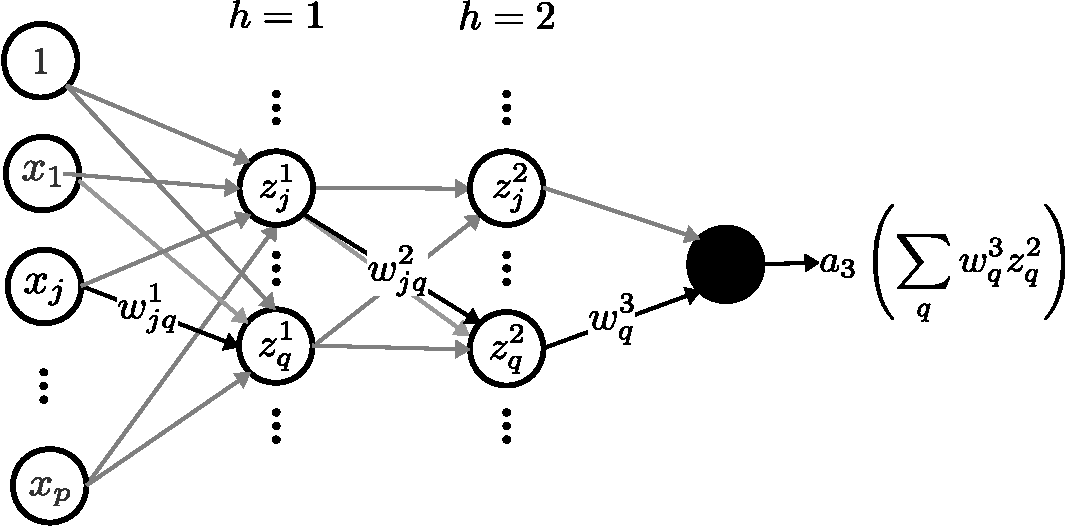
\includegraphics[width=0.8\textwidth]{figures/nonlin/mlp}
  \caption{Architecture d'un perceptron multi-couche. }
  \label{fig:mlp}
\end{figure}

\paragraph{Nombre de param�tres} Le perceptron multi-couche est un mod�le
param�trique dont les param�tres sont les poids de connexions $w_{jq}^h$. Le
nombre de couches et leurs nombres de neurones font partie des hyperparam�tres
: on les suppose fix�s, ce ne sont pas eux que l'on apprend. Ce mod�le a donc
d'autant plus de param�tres (c'est-�-dire de poids de connexion) qu'il y a de
couches interm�diaires et de neurones dans ces couches. Cela leur conf�re une
grande puissance de mod�lisation (voir plus de d�tails � la
section~\ref{sec:universal_approx}), mais le risque de surapprentissage est
�lev�.  Les r�seaux de neurones profonds requi�rent ainsi souvent des quantit�s
massives de donn�es pour apprendre de bons mod�les.

\subsection{Entra�nement d'un perceptron multi-couche}
Il est important de remarquer que la minimisation du risque empirique pour un
perceptron multi-couche n'est {\it pas} un probl�me d'optimisation
convexe. Ainsi, nous n'avons pas d'autres choix que d'utiliser un algorithme �
directions de descente, sans aucune garantie de converger vers un minimum
global.

L'initialisation des poids de connexion, la standardisation des variables, le
choix de la vitesse d'apprentissage et celui des fonctions d'activation ont
tous un impact sur la capacit� du perceptron multi-couche � converger vers une
bonne solution. Entra�ner un r�seau de neurones multi-couche n'est pas chose
ais�e.

\paragraph{R�tropropagation} N�anmoins, le principe fondamental de
l'apprentissage d'un perceptron multi-couche, connu sous le nom de
\textbf{r�tropropagation} ou {\it backpropagation} (souvent raccourci en {\it
  backprop}), est connu depuis des d�cennies. Il repose, comme pour le
perceptron sans couche interm�diaire, sur l'utilisation de l'algorithme du
gradient pour minimiser, � chaque nouvelle observation, le risque
$L(f(\xx^i), y^i)$. Pour plus de d�tails, reportez-vous � la
section~\ref{sec:backprop}.
  
\subsection{Deep learning}
Le domaine de l'\textbf{apprentissage profond} repose
fondamentalement sur les principes que nous venons de voir. En effet, un
perceptron multi-couche est profond d�s lors qu'il contient suffisamment de
couches -- la d�finition de \og suffisamment \fg~d�pendant des auteurs.  Le
domaine de l'apprentissage profond s'int�resse aussi � de nombreuses autres
architectures comme les \textbf{r�seaux r�currents} ({\it RNN}, pour {\it
  Recursive Neural Nets}), et en particulier {\it Long Short-Term Memory (LSTM)
  networks} pour mod�liser des donn�es s�quentielles (telles que du texte ou
des donn�es temporelles) et les \textbf{r�seaux convolutionnels} ({\it CNN},
pour {\it Convolutional Neural Nets}) pour le traitement d'images.

Dans tous les cas, il s'agit essentiellement d'utiliser ces architectures pour
cr�er des mod�les param�triques (potentiellement tr�s complexes), puis d'en
apprendre les poids par un algorithme � directions de descente.

L'apprentissage des poids de connexion d'un r�seau de neurones profond pose des
difficult�s techniques : en effet, le probl�me d'optimisation � r�soudre n'est
pas convexe, et converger vers un \og bon \fg~minimum local n'est pas une t�che
facile. Cette t�che est d'autant plus difficile que le r�seau est complexe, et
les progr�s dans ce domaine ne sont possibles que gr�ce au d�veloppement de
m�thodes pour la rendre plus ais�e.

Une des techniques les plus importantes dans ce domaine est le
\textbf{pr�-entra�nement}, ou \textit{pretraining} : il s'agit d'utiliser un
r�seau de neurones profond entra�n� sur une tr�s grosse base de donn�es de m�me
nature que le probl�me que l'on cherche � r�soudre pour initialiser
l'optimisation sur notre jeu de donn�es. Par exemple, pour une t�che de
classification sur un jeu de donn�es de quelques milliers d'images m�dicales,
on partira d'un r�seau de neurones entra�n� sur une base de donn�es d'images
naturelles telle que ImageNet, qui contient des millions d'images appartenant �
plus de 20\,000 classes.

De plus, les r�seaux de neurones profonds ont de nombreux param�tres, et
requi�rent donc l'utilisation de grands volumes de donn�es pour �viter le
sur-apprentissage. Il est donc g�n�ralement n�cessaire de les d�ployer sur des
architectures distribu�es.

Ainsi, malgr� son succ�s dans certains domaines d'application (notamment
images, texte, et s�ries temporelles), le \textit{deep learning} est d�licat �
mettre en place et n'est pas toujours la meilleure solution pour r�soudre un
probl�me de \textit{machine learning}, en particulier face � un petit jeu de
donn�es.

\paragraph{Apprentissage de repr�sentations $\bigstar$}
On associe souvent aux r�seaux de neurones profond la notion de {\it
  representation learning}. En effet, il est possible de consid�rer que chacune
des couches interm�diaires successives apprend une nouvelle repr�sentation des
donn�es $(z^h_1, z^h_2, \dots, z^h_{p_h})$ � partir de la repr�sentation de la
couche pr�c�dente, et ce jusqu'� pouvoir appliquer entre la derni�re couche
interm�diaire et la sortie du r�seau un algorithme lin�aire.


\section{M�thodes � noyaux}
Les m�thodes � noyaux permettent de construire des mod�les non-lin�aires de
r�gression ou de classification sur le m�me mod�le que la r�gression
polynomiale, mais sans avoir � calculer explicitement les nouvelles variables.

Nous allons tout d'abord illustrer leur principe sur l'exemple de la r�gression ridge.

\subsection{Exemple de la r�gression ridge quadratique}

\paragraph{R��criture de la r�gression ridge}
Nous utilisons ici les m�mes notations qu'� la section~\ref{sec:ridge_regression}.
La fonction de pr�diction de la r�gression ridge est de la forme
\begin{equation}
  \label{eq:reg_ridge_pred}
  f(\xx) = \langle \xx,  \bbeta^* \rangle,
\end{equation}
o� $\bbeta^*$ est donn� par l'�quation~\eqref{eq:ridgereg_sol} :
\begin{equation}
  \label{eq:reg_ridge_beta}
  \bbeta^* =  \left( \lambda I_p + X^\top X  \right)^{-1} X^\top \yy.
\end{equation}
% Ici $X \in \RR^{n \times p}$ est la matrice de design potentiellement
% augment�e d'une colonne de 1 selon la transformation~\eqref{eq:added_ones}.
  
En rempla�ant $\bbeta^*$ par sa valeur, l'�quation~\eqref{eq:reg_ridge_pred} peut se r��crire comme 
\begin{equation}
  \label{eq:reg_ridge_2}
  f(\xx) = \xx X^\top (\lambda I_n + XX^\top)^{-1} y.
\end{equation}
Vous en trouverez la preuve section~\ref{sec:ridge_rewrite}.


Nous allons maintenant traiter l'exemple de la \textbf{r�gression ridge
  quadratique}, c'est-�-dire d'une r�gression polynomiale de degr� 2
r�gularis�e par un terme $\ell_2$. 
D�finissons l'application
\begin{align*}
  % \phi: \RR^p & \rightarrow \RR^{{d+p \choose p}} \\
  % (x_1, x_2, \dots, x_p)  &  \mapsto
  %                           (x_1, x_2, \dots, x_p,~x_1^2, x_1 x_2, \dots,
  %                           x_p^2, \dots, x_1^d, x_1^{d-1}  x_2, \dots, x_p^d ).
  \phi: \RR^p & \rightarrow \RR^{m} \\
  (x_1, x_2, \dots, x_p)  &  \mapsto
                            (1, \sqrt{2} x_1, \sqrt{2} x_2, \dots, \sqrt{2} x_p,~x_1^2, x_1 x_2, \dots,
                            x_p^2),
\end{align*}
avec $m = 1+ p + \frac12 p(p+1)$ le nombre de monomes de $p$ variables de degr�
au plus $2$.  Les coefficients $\sqrt{2}$ sont introduits ici pour des
facilit�s de calcul plus tard ; ils ne changent rien conceptuellement.

La fonction de d�cision d'une r�gression quadratique est ainsi une fonction
\textit{lin�aire} en $\phi(\xx)$ : la r�gression polynomiale est �quivalente �
une r�gression lin�aire sur un espace de plus grande dimension.  

Pour entra�ner une r�gresion ridge polynomiale, nous pouvons donc entra�ner une
r�gression ridge sur les donn�es $\{(\phi(\xx^1), y^1), (\phi(\xx^2), y^2), \dots, (\phi(\xx^n), y^n)\}.$ Posons donc $\Phi \in \RR^{n \times m}$ la matrice
d�crivant les images observations $(\xx^1, \xx^2, \dots, \xx^n)$ par $\phi$.

L'�quation~\eqref{eq:reg_ridge_2} devient alors
\begin{equation}
  \label{eq:reg_ridge_phi}
  f_\phi(\xx) = \phi(\xx) \Phi^\top (\lambda I_n + \Phi \Phi^\top)^{-1} y.
\end{equation}

D�finissons maintenant la fonction
\begin{eqnarray*}
  k: \RR^p \times \RR^p & \rightarrow & \mathbb{R} \\
  \xx,~\xx' & \mapsto & \innerproduct{\phi(\xx),~\phi(\xx')}.
\end{eqnarray*}

Construisons le vecteur $\kappa \in \RR^n$ dont la
$i$-�me entr�e est
% \begin{equation*}
  $\kappa_i = \innerproduct{\phi(\xx),~\phi(\xx^i)} = k(\xx, \xx^i)$,
% \end{equation*}
et la matrice $K \in \RR^{n \times n}$ dont l'entr�e $K_{il}$ est
% \begin{equation*}
$K_{il} = \innerproduct{\phi(\xx^i),~\phi(\xx^l)} = k(\xx^i, \xx^l).$
% \end{equation*}

Nous pouvons maintenant r��crire l'�quation~\eqref{eq:reg_ridge_phi} comme
\begin{equation}
  \label{eq:reg_ridge_k}
  f_\phi(\xx) =  \kappa (\lambda I_n + K)^{-1} y,
\end{equation}
dans laquelle $\phi$ n'apparait plus que dans des produits scalaires (calcul de $\kappa$
et $K$).

Cela signifie que nous pouvons apprendre une r�gression ridge quadratique sans utiliser $\phi$, � condition de conna�tre $k$.

Cette phrase peut para�tre surprenante, car nous avons d�fini $k$ en utilisant $\phi$.

Cependant, pour tout $\xx$ et $\xx^\prime$ de $\RR^p$,
\begin{equation*}
  k(\xx,~\xx^\prime) = \left(\innerproduct{\xx,~\xx^\prime} + 1 \right)^2.
\end{equation*}

Il est donc possible d'apprendre une r�gression ridge quadratique sans calculer
explicitement les images des $\xx^i$ ou de l'observation $\xx$ � �tiqueter dans
$\RR^m$.

Cela a un int�r�t calculatoire. En effet, calculer $\phi(\xx)$ puis
$\phi(\xx^\prime)$ puis leur produit scalaire requiert de l'ordre de
$2m + 2m = 2 + 2p + p(p+1)$ op�rations. � l'inverse, calculer
$\innerproduct{\xx,~\xx^\prime}$ puis ajouter 1 et �lever le tout au carr�
requiert $p+2$ op�rations : la deuxi�me option est moins co�teuse. �videmment,
pour une r�gression quadratique et un faible nombre de variables, ces deux
valeurs sont toutes les deux faibles. Cependant, la diff�rence de temps de calcul entre les deux approches va augmenter avec le nombre de variables et le degr� de polyn�me consid�r�.
% Cependant, vous pouvez imaginer �tendre
% cette approche � n'importe quel degr� $d$, en d�finissant
% $k(\xx,~\xx^\prime) = \left(\innerproduct{\xx,~\xx^\prime} + 1 \right)^d$, ce
% qui correspond � une fonction $\phi$ calculant les ${d+p \choose p}$ monomes de
% $p$ variables de degr� au plus $d$. La diff�rence de temps de calcul entre les
% deux approches va se creuser quand $p$ et $d$ augmentent.

La d�marche que nous avons pr�sent�e ici se g�n�ralise �
\begin{itemize}
\item n'importe quelle fonction $k$ de deux variables s'�crivant sous la forme
  d'un produit scalaire d'images de ces variables dans un espace de
  Hilbert\footnote{� savoir, un espace de dimension potentiellement infinie et
    muni d'un produit scalaire ; il s'agit d'une g�n�ralisation des espaces
    euclidiens. Vous pouvez consid�rer qu'un espace de Hilbert est $\RR^m$ ou
    $\mathbb{C}^m$, avec potentiellement � $m = +\infty$ �.} ;
\item n'importe quelle proc�dure d'apprentissage dans laquelle les observations
  n'apparaissent que sous la forme de produits scalaires entre observations.
\end{itemize}
C'est ce que nous faisons dans la section suivante.

\subsection{M�thodes � noyau}
\label{sec:kernels}

\paragraph{Noyau} On appelle \textbf{noyau} sur un espace quelconque $\XX$ toute
fonction $k: \XX \rightarrow \RR$ continue, sym�trique et semi-d�finie
positive\footnote{au sens o�
pour tout $N \in \NN$, pour tout $(\xx^1, \xx^2, \dots \xx^N) \in
  \mathcal{X}^N$ et pour tout $(a_1, a_2, \dots a_N) \in \RR^N$, 
  $\sum_{i=1}^N \sum_{l=1}^N a_i a_l k(\xx^i, \xx^l) \geq 0$. En particulier, la matrice $K$ d�finie � la section pr�c�dente est ainsi semi-d�finie positive.}.\\
Le \textbf{th�or�me de Moore-Aronszajn}\footnote{D�montr� dans \textit{Theory
    of reproducing kernels}, N. Aronszajn, Transactions of the American
  Mathematical Society 68(3):337--40 (1950), et attribu� � E. Hastings Moore.}
garantit alors l'existence d'un espace de Hilbert $\HH$ et d'une application
$\phi: \XX \rightarrow \HH$ telle que pour tout
$(\xx, \xx^\prime) \in \XX \times \XX,$
$k(\xx,~\xx^\prime) = \innerproduct{\phi(\xx),~\phi(\xx^\prime)}_\HH.$\\
Nous
appellerons $\HH$ l'\textbf{espace de redescription}, car il permet de d�crire les �l�ments de $\XX$ avec de nouvelles variables.

\paragraph{Astuce du noyau} �tant donn�e une proc�dure d'apprentissage
automatique dans laquelle les observations n'apparaissent que dans des produits
scalaires entre observations, on peut remplacer tous les produits scalaires en
question par un noyau. Cela revient � appliquer la m�me proc�dure
d'apprentissage dans l'espace de redescription.\\
Cela signifie que nous n'avons pas besoin de faire de calculs dans $\HH$, qui
est g�n�ralement de tr�s grande dimension : c'est ce que l'on appelle
\textbf{l'astuce du noyau.} Elle s'applique non seulement � la r�gression
ridge, mais aussi � de nombreux autres algorithmes d'apprentissage, dont les
SVM (vues dans la PC~6), ce que vous pouvez lire en plus de d�tails dans la section~\ref{sec:kernel_svm}.

Quand on applique l'astuce du noyau � la r�gression ridge, on parle de
\textbf{r�gression ridge � noyau} ou \textit{kernel ridge regression (KRR)} en
anglais.


Le \textbf{noyau polynomial} de degr� $d \in \NN$,
d�fini sur $\RR^p \times \RR^p$ par
$k(\xx, \xx') = \left( \langle \xx, \xx' \rangle + c\right)^d,$ o� $c \in \RR$
permet d'inclure des termes de degr� inf�rieur � $d$, correspond � un espace de
redescription $\HH$ comptant autant de dimensions qu'il existe de mon�mes de
$p$ variables de degr� inf�rieur ou �gal � $d$, soit $p+d \choose d$.

Encore plus puissant, le \textbf{noyau radial gaussien}, ou {\it noyau RBF}
(pour {\it Radial Basis Function}), de bande passante $\sigma > 0,$ et d�fini
sur $\RR^p \times \RR^p$ par
$k(\xx, \xx^\prime) = \exp\left( - \frac{||\xx - \xx^\prime||^2}{2 \sigma^2}
\right),$ correspond � un espace de redescription $\HH$ de dimension {\it
  infinie}, ce qui se d�montre en utilisant le d�veloppement en s�rie enti�re
de la fonction exponentielle (voir d�tails section~\ref{sec:rbf_kernel}).Ainsi,
l'�quation~\eqref{eq:reg_ridge_k} o� $\kappa$ et $K$ ont �t� calcul�s avec le
noyau RBF ci-dessus permet d'apprendre une r�gression polynomiale de degr�
arbitrairement grand.

Vous trouverez plus d'exemples de noyaux dans la section~\ref{sec:more_kernels}.


\section{Arbres et for�ts}
� l'exception de l'algorithme des $k$ plus proches voisins (cf. PC~4), les
algorithmes d'apprentissage supervis� que nous avons vus jusqu'� pr�sent
permettent d'apprendre des mod�les param�triques. Les arbres de d�cision sont
un autre exemple de mod�le simple et non-param�trique \footnote{Les mod�les
  appris par des m�thodes � noyau sont aussi non-param�triques : il n'y a plus
  d'hypoth�se sur la distribution de $(X, Y)$. La complexit� d'un mod�le �
  noyau augmente avec le nombre d'observations.}.

\subsection{Arbres de d�cision}
On appelle \textbf{arbre de d�cision} (\textit{decision tree} en anglais) un
mod�le pr�dictif qui peut �tre repr�sent� sous la forme d'un arbre. Chaque
n{\oe}ud de l'arbre teste une condition sur une variable et chacun de ses
enfants correspond � une r�ponse possible � cette condition. Les feuilles de
l'arbre correspondent � une �tiquette.

Pour pr�dire l'�tiquette d'une observation, on \og suit \fg~les r�ponses aux
tests depuis la racine de l'arbre, et on retourne l'�tiquette de la feuille �
laquelle on arrive.

Ils sont couramment utilis�s en dehors du monde du machine learning, par
exemple pour d�crire les �tapes d'un diagnostic ou d'un choix de traitement
pour un m�decin, ou les chemins possibles dans un \og livre dont vous �tes le
h�ros \fg. La figure~\ref{fig:fruit_tree} pr�sente un tel arbre de d�cision.

Les arbres de d�cision permettent de traiter naturellement des variables
qualitatives.

Ils permettent aussi de traiter des classes
multi-modales (comme ici pour l'�tiquette \og pomme \fg, qui est affect�e � un
fruit grand et rouge ou � un fruit jaune et rond.)


\begin{figure}[h]
  \centering
  \includegraphics[width=0.5\textwidth]{figures/nonlin/fruit_tree}
  \caption{Exemple d'arbre de d�cision pour classifier des fruits entre pommes
    (+) et autres (-).}
  \label{fig:fruit_tree}
\end{figure}



\subsection{Comment faire pousser un arbre de d�cision (cas binaire)}
\label{sec:grow_tree_binary}
L'algorithme utilis� pour entra�ner un arbre de d�cision est appel�
\textbf{CART}, pour {\it Classification And Regression Tree}. Il s'agit d'un
algorithme de partitionnement de l'espace par une approche gloutonne, r�cursive
et divisive.

Dans cette section, nous expliquons comment entra�ner un arbre de d�cision pour
un probl�me de classification binaire sur des variables binaires : on consid�re
$\YY = \{0, 1\}$ et $x_j \in \{0, 1\}$ pour tout $j=1, \dots, p$.

� chaque n{\oe}ud d'un arbre de d�cision construit par CART correspond une
\textbf{variable s�paratrice} ({\it splitting variable})
$j \in \{1, \dots, p\}$ selon laquelle vont �tre partitionn�es les
donn�es. Cette variable s�paratrice d�finit deux r�gions, correspondant aux
enfants du n{\oe}ud consid�r� :
\begin{equation*}
  R_l(j) = \{\xx~|~x_j = 0\} ; \hspace{2em} 
  R_r(j) =  \{\xx~|~x_j = 1\}.
\end{equation*}
Au niveau de la racine de l'arbre, $R_l$ et $R_r$ partitionnent l'ensemble des
observations. Ensuite, chaque n{\oe}ud partitionne uniquement les observations
qui sont arriv�es jusqu'� lui, autrement dit qui v�rifient toutes les
conditions dict�es par ses parents.


On peut alors associer, au niveau de ce n{\oe}ud, l'�tiquette majoritaire de la
r�gion $R_l(j)$ � tous les individus de $R_l(j)$ et l'�tiquette majoritaire de
la r�gion $R_r(j)$ � tous les individus de $R_r(j)$.

\paragraph{Exemple} Sur l'exemple de la figure~\ref{fig:fruit_tree}, il
s'agirait par exemple au n{\oe}ud � incurv� � $R_l$ l'ensemble des fruits non
rouge et de forme incurv�e, et $R_r$ l'ensemble des fruits non rouge et de
forme non incurv�e. Si la majorit� des individus de $R_l$ ne sont pas des
pommes, on associe alors l'�tiquette n�gative � tous les individus de $R_l$. Si
la majorit� des individus de $R_r$ sont des pommes, on associe alors
l'�tiquette positive � tous les individus de $R_r$ (malgr� la pr�sence de
citrons dans $R_r$, qui ne seront identifi�s qu'au n{\oe}ud suivant).

� chaque it�ration de CART, on it�re sur toutes les valeurs possibles de $j$
pour d�terminer celle qui minimise localement l'erreur faite en attribuant �
toutes les observations d'une r�gion l'�tiquette majoritaire dans cette r�gion.
Il s'agit donc bien d'un probl�me de minimisation du risque
empirique. Cependant, il s'agit d'un algorithme glouton : il n'y a aucune
garantie que cette strat�gie aboutisse � l'arbre de d�cision dont l'erreur sur
le jeu d'entra�nement est minimale.

\paragraph{Formalisation $\bigstar$} On peut formellement noter :
\begin{equation}
  \argmin_{j \in \{1, \dots, p\}} \left( 
    \frac1{\abs{R_l(j)}} \sum_{i: \xx^i \in R_l(j)} L(y_l(j), y^i)  + 
     \frac1{\abs{R_r(j)}} \sum_{i: \xx^i \in R_r(j)} L(y_r(j), y^i)
   \right)
   \label{eq:erm_binary_tree}
\end{equation}
avec $y_l(j)$ l'�tiquette majoritaire dans $R_l(j)$, � savoir
\begin{equation*}
y_l(j) = \argmax_{c \in \{0, 1\}} \abs{\{i:\xx^i \in R_l(j) ~|~y^i=c\}},
\end{equation*}
et, similairement, 
$y_r(j)$ l'�tiquette majoritaire dans $R_r(j)$, � savoir
\begin{equation*}
y_r(j) = \argmax_{c \in \{0, 1\}} \abs{\{i:\xx^i \in R_r(j) ~|~y^i=c\}}.
\end{equation*}


La section~\ref{sec:impurity} donne plus de d�tail sur la fonction de perte $L$
utilis�e dans le cas des arbres de d�cision. Vous pouvez consid�rer qu'on
utilise l'erreur de classification.

La section~\ref{sec:grow_tree} montre comment �tendre ce principe � des
probl�mes de r�gression et � des variables discr�tes (de plus de deux
modalit�s) ou continues. Il s'agit
\begin{itemize}
\item pour traiter les variables non-binaires, de les binariser (pour une variable continue, il s'agira de les comparer � un seuil) ;
\item pour traiter la r�gression, de remplacer le vote de la majorit� par une
  moyenne.
\end{itemize}

Malheureusement, les arbres de d�cision ont tendance � donner des mod�les trop
simples et � avoir des performances de pr�diction � peine sup�rieures � des
mod�les al�atoires et peu robustes aux variations dans les donn�es. On les
qualifie d'\textbf{apprenants faibles} ({\it weak learners} en
anglais). Heureusement, il est possible d'y rem�dier gr�ce aux m�thodes
ensemblistes.

\subsection{Comment faire pousser un arbre de d�cision (cas g�n�ral) $\bigstar$}
\label{sec:grow_tree}
Dans le cas o� la variable de s�paration est une variable {\it discr�te}
pouvant prendre plus de deux valeurs (ou modalit�s), elle s'accompagne alors
d'un sous-ensemble de ces valeurs $\Scal \subset \text{dom}(x_j).$ Les deux
r�gions sont
\begin{equation*}
  R_l(j, \Scal) = \{\xx~|~x_j \in \Scal\} ; \hspace{2em} 
  R_r(j, \Scal) = \{\xx~|~x_j \notin  \Scal\}.
\end{equation*}

Dans le cas o� la variable de s�paration est une variable {\it r�elle},
elle s'accompagne alors d'un \textbf{point de s�paration} ({\it splitting
  point}) $s$ qui est la valeur de la variable par rapport � laquelle va se
faire la d�cision. Les deux r�gions sont alors
\begin{equation*}
  R_l(j, s) = \{\xx~|~x_j < s\} ; \hspace{2em} R_r(j, s) = \{\xx~|~x_j \geq s\}.
\end{equation*}
Si l'on suppose les valeurs prises par la variable $j$ dans $\DD$ ordonn�es :
$x_j^1 \leq x_j^2 \leq \dots, \leq x_j^n$, alors les valeurs possibles de $s$
sont $\frac{x^{i+1}_j - x^i_j}2$ pour toutes les valeurs de $i$ telles que
$x^{i+1}_j \neq x^i_j.$


� chaque it�ration de l'algorithme CART, on it�re sur toutes les valeurs
possibles de $j$ et, le cas �ch�ant, toutes les valeurs possibles de $s$ ou
$\Scal$ pour d�terminer celle qui minimise localement l'erreur faite en
attribuant � toutes les observations de la r�gion de gauche $(R_l)$ (resp. de
droite $(R_r)$) leur �tiquette majoritaire (dans le cas d'un probl�me de
classification) ou moyenne (dans le cas d'un probl�me de r�gression).


Formellement, notons $\Ical$ l'ensemble des variables de
s�parations possibles, � savoir l'union
\begin{itemize}
\item des indices $j$ des variables binaires ;
\item des couples $(j, \Scal)$ de paires de variables discr�tes � plus de deux
  modalit�s, et de tous les sous-ensembles $\Scal$ possible de ces modalit�s ;
\item des couples $(j, s)$ de paires de variables continues et des points de
  s�paration possibles.
\end{itemize}
Nous noterons donc ainsi $\zeta \in \Ical$ une variable de s�paration,
accompagn�e si elle est discr�te d'un sous-ensemble $\Scal$ de valeurs ou si
elle est continue d'un seuil $s$, ce qui nous permet de noter $R_l(\zeta)$ et
$R_r(\zeta)$ les deux r�gions d�finies par $\zeta$ ind�pendamment de sa nature
binaire, discr�te ou continue.

Notons maintenant
\begin{equation*}
  y_l(\zeta) =
  \begin{cases}
    \argmax_{c \in \{0, 1\}} \abs{\{i:\xx^i \in R_l(\zeta) ~|~y^i=c\}} & \text{ pour un probl�me de classification binaire } \\
    \frac1{\abs{\{i:\xx^i \in R_l(\zeta)\}}} \sum_{i:\xx^i \in R_l(\zeta)} y^i & \text{ pour un probl�me de r�gression.}
  \end{cases}
\end{equation*}

on g�n�ralise alors l'�quation~\eqref{eq:erm_binary_tree} en :
\begin{equation}
  \argmin_{\zeta \in \Ical} \left( 
    \frac1{\abs{R_l(\zeta)}} \sum_{i: \xx^i \in R_l(\zeta)} L(y_l(\zeta), y^i)  + 
     \frac1{\abs{R_r(\zeta)}} \sum_{i: \xx^i \in R_r(\zeta)} L(y_r(\zeta), y^i)
  \right)
\end{equation}

Dans le cas d'un probl�me de r�gression, la fonction de perte $L$ est, encore
une fois, l'erreur quadratique moyenne. Dans le cas d'un probl�me de
classification, plusieurs choix sont possibles. Ces choix sont
d�taill�s dans la section~\ref{sec:impurity}.

Ainsi, avec beaucoup d'�chantillons et beaucoup de variables continues, un
arbre de d�cision peut �tre long � entra�ner : il faut � chaque n{\oe}ud tester
toutes les variables et chacun de leur seuils, ce qui fait de l'ordre de $np$
op�rations par n{\oe}ud.


\subsection{M�thodes ensemblistes}
Les m�thodes ensemblistes sont des m�thodes tr�s puissantes en pratique, qui
reposent sur l'id�e que combiner de nombreux apprenants faibles permet
d'obtenir une performance largement sup�rieure aux performances individuelles
de ces apprenants faibles, car leurs erreurs se compensent les unes les autres.

Les m�thodes ensemblistes sont particuli�rement pertinentes lorsque les mod�les
que l'on combine ont �t� appris par des apprenants faibles, c'est-�-dire
simples � entra�ner et peu performants.  En pratique, si les mod�les
individuels sont d�j� performants et robustes au bruit, le mod�le ensembliste
ne sera pas n�cessairement meilleur. On utilise le plus souvent des arbres de
d�cision comme mod�les individuels.

% Cette id�e est similaire au concept de \textbf{sagesse des foules}, ou {\it
%   wisdom of crowd} : si je demande � mes �l�ves l'ann�e de la mort de Georges
% Pompidou, il est probable que la moyenne de leurs r�ponses soit assez proche de
% la bonne (1974) ; cependant, si je demande cette date � une seule personne au
% hasard, je n'aurais aucun moyen de savoir a priori si cette personne conna�t la
% date ou me r�pond au hasard.

\begin{exemple}
  Pour illustrer ce concept, imaginons une t�che de classification en deux
  dimensions, dans laquelle les deux classes sont s�par�es par une diagonale,
  mais que le seul algorithme d'apprentissage dont nous disposions ne puisse
  apprendre qu'une fronti�re de d�cision en escalier, avec un nombre limit� de
  paliers. Combiner des dizaines voire des centaines de ces fronti�res de
  d�cision en escalier peut nous donner une bien meilleure approximation de la
  v�ritable fronti�re de d�cision. Cet exemple est illustr� sur la
  figure~\ref{fig:crowd_diagonal}.
\end{exemple}

\begin{figure}[h]
  \centering
  \includegraphics[width=0.4\textwidth]{figures/nonlin/crowd_diagonal}
  \caption{Chacune des fronti�res de d�cision en escalier est une mauvaise
    approximation de la vraie fronti�re qui est la diagonale en trait
    plein. Cependant, combiner ces escalier permet une meilleure
    approximation de la diagonale.}
  \label{fig:crowd_diagonal}
\end{figure}


\subsection{Bagging} Mais comment cr�er {\it plusieurs} arbres de d�cision
diff�rents � partir d'un unique jeu de donn�es ? Le \textbf{bagging} est une
m�thode parall�le, bas�e sur le r�-�chantillonnage, qui permet de cr�er des
arbres ind�pendants les uns des autres.

Il consiste � former $B$ versions de $\DD$ par \textbf{�chantillonage
  bootstrap}, autrement dit en tirant $n$ exemples de $\DD$ {\it avec
  remplacement}. Ainsi, chaque exemple peut appara�tre plusieurs fois, ou pas
du tout, dans $\DD_b$.

La probabilit� que $(\xx^i, y^i)$ apparaisse dans $\DD_b$ peut �tre calcul�e
comme le compl�mentaire � 1 de la probabilit� que $(\xx^i, y^i)$ ne soit tir�
aucune des $n$ fois. La probabilit� de $(\xx^i, y^i)$ soit tir� une fois vaut
$\frac1n$. Ainsi
\begin{equation*}
  \PP[(\xx^i, y^i) \in \DD_b] = 1 - \left(1 - \frac1n\right)^n.
\end{equation*}
Quand $n$ est grand, cette probabilit� vaut donc environ
$1 - e^{-1} \approx 0.632$, car la limite en $+\infty$ de
$\left(1 + \frac{x}{n}\right)^n$ vaut $e^x$.  Ainsi, $\DD_b$ contient environ
deux tiers des observations de $\DD$.


Chaque arbre est entra�n� sur un de ces �chantillons boostrap, ce qui peut �tre
fait en parall�le. Les $B$ pr�dictions sont ensuite combin�es
\begin{itemize}
\item par vote de la majorit� dans le cas d'un probl�me de classification ; 
\item en prenant la moyenne dans le cas d'un probl�me de r�gression.
\end{itemize}

\subsection{For�ts al�atoires}
La puissance des m�thodes ensemblistes se r�v�le lorsque les apprenants faibles
sont ind�pendants conditionnellement aux donn�es, autrement dit aussi
diff�rents les uns des autres que possible, afin que leurs erreurs puissent se
compenser les unes les autres. Pour atteindre cet objectif, l'id�e des
\textbf{for�ts al�atoires} (ou \textit{random forests}) est de construire les
arbres individuels non seulement sur des �chantillons diff�rents (comme pour le
bagging), mais aussi en utilisant des {\it variables} diff�rentes.

Plus pr�cis�ment, les arbres construits pour former une for�t al�atoire
diff�rent de ceux appris par CART en ce que, � chaque n{\oe}ud, on commence par
s�lectionner $q < p$ variables al�atoirement, avant de choisir la variable
s�paratrice {\it parmi celles-ci}. En classification, on utilise typiquement
$q \approx \sqrt{p}$, ce qui permet aussi de r�duire consid�rablement les temps
de calculs puisqu'on ne consid�re que peu de variables � chaque n{\oe}ud (5
pour un probl�me � 30 variables, 31 pour un probl�me avec 1000 variables). Pour
la r�gression, le choix par d�faut est plut�t de $q \approx \frac{p}3.$ Ces
valeurs sont bas�es sur la pratique ; la th�orie des for�ts al�atoires est
toujours tr�s peu d�velopp�e, bien que cette m�thode ait �t� propos�e il y a
une vingtaine d'ann�es.


\section{Compl�ments $\bigstar$}

\subsection{Classification binaire avec un perceptron}
\label{sec:perceptron_binary}
\paragraph{Mod�le}
Dans le cas d'un probl�me de classification binaire, on peut aussi utiliser
directement une fonction de seuil :
\begin{equation}
  \label{eq:seuil}
  f: \xx \mapsto 
  \begin{cases}
    0 & \text{ si } o(\xx) \leq 0 \\
    1 & \text{ sinon.}
  \end{cases}
\end{equation}

\paragraph{Fonction de co�t} On utilise alors une fonction de co�t connue sous le nom de \textbf{crit�re du
  perceptron} :
\begin{equation}
  \label{eq:perceptron}
  L(f(\xx^i), y^i) = \max(0, - y^i o(\xx^i)) = 
  \max(0, - y^i \innerproduct{\ww,~\xx})
\end{equation}
Ce crit�re est proche de la fonction d'erreur hinge (voir section 2.2 de la
PC~6). Quand la combinaison lin�aire des entr�es a le bon signe, le crit�re du
perceptron est nul. Quand elle a le mauvais signe, le crit�re du perceptron est
d'autant plus grand que cette combinaison lin�aire est �loign�e de 0.

\paragraph{Entra�nement}
En utilisant ce crit�re, la r�gle d'actualisation~\eqref{eq:update_rule}
devient :
\begin{equation*}
  \label{eq:update_rule_binclass}
  w_j \leftarrow \begin{cases}
    0 & \text{ si } y^i o(\xx^i) > 0 \\
    - y^i x_j^i & \text{ sinon.}
  \end{cases}
\end{equation*}
Ainsi, quand le perceptron fait une erreur de pr�diction, il d�place la
fronti�re de d�cision de sorte � corriger cette erreur.

% Le \textbf{th�or�me de convergence du perceptron}\footnote{\textit{On
%     convergence proofs on perceptrons}, A.  B. J. Novikoff.  Symposium on the
%   Mathematical Theory of Automata, 615--622 (1962).} �nonce que �tant donn� un
% jeu de $n$ observations �tiquet�es $\DD = \{(\xx^i, y^i)_{i=1, \dots, n}\}$ et
% $D, \gamma \in \RR_+^*$, si :
% \begin{itemize}
% \item $\forall i=1, \dots, n$, \; $\ltwonorm{\xx^i} \leq D$
% \item il existe $\uu \in \RR^{p+1}$ tel que 
%   \begin{itemize}
%   \item $\ltwonorm{\uu}=1$ et
%   \item $\forall i=1, \dots, n$, \;
%     $y^i \langle \uu, \xx \rangle \geq \gamma$
%   \end{itemize}
% \end{itemize}
% alors l'algorithme du perceptron converge en au plus
% $\left(\frac{D}{\gamma}\right)^2$ �tapes.




\subsection{Approximation universelle}
\label{sec:universal_approx}
\paragraph{Th�or�me de l'approximation universelle} 
Soit $a: \RR \rightarrow \RR$ une fonction non constante, born�e, continue et
croissante et $K$ un sous-ensemble compact de $\RR^P$. �tant donn�
$\epsilon > 0$ et une fonction $f$ continue sur $K$, il existe un entier $m$,
$m$ scalaires $\{d_i\}_{i=1, \dots, m}$, $m$ scalaires
$\{b_i\}_{i=1, \dots, m}$, et $m$ vecteurs $\{\ww_i\}_{i=1, \dots, m}$ de
$\RR^p$ tels que pour tout $\xx \in K$,
\begin{equation*}
  \lvert f(\xx) - \sum_{i=1}^m d_i \; a \left( \langle \ww_i, \xx \rangle + 
    b_i \right) \rvert < \epsilon.
\end{equation*}
En d'autres termes, toute fonction continue sur un sous-ensemble compact de
$\RR^p$ peut �tre approch�e avec un degr� de pr�cision arbitraire par un
perceptron multi-couche � une couche interm�diaire contenant un nombre fini
de neurones.

  
Ce th�or�me\footnote{Initialement d�montr� dans \textit{Approximation by
    superpositions of a sigmoidal function}, G. Cybenko. Mathematics of
  Control, Signals and Systems, 2(4):303--314 (1989) et affin� dans
  \textit{Approximation capabilities of multilayer feedforward networks,}
  K. Hornik, Neural Networks 4(2):241--257 (1991).}  montre la puissance de
mod�lisation du perceptron multi-couche. Cependant, ce r�sultat ne nous donne
ni le nombre de neurones qui doivent composer cette couche interm�diaire, ni
les poids de connexion � utiliser. Les r�seaux de neurones � une seule couche
cach�e sont g�n�ralement peu efficaces, et on aura souvent de meilleurs
r�sultats en pratique avec plus de couches.


\subsection{R�tropropagation}
\label{sec:backprop}
Pour actualiser le poids de connexion $w^h_{jq}$ du neurone $j$ de la couche
$h-1$ vers le neurone $q$ de la couche $h$, nous devons calculer
$\frac{\partial L(f(\xx^i, y^i))}{\partial w^h_{jq}}.$ Pour ce faire, nous
pouvons appliquer le th�or�me de d�rivation des fonctions compos�es ({\it chain
  rule} en anglais). Nous notons $o^h_j$ la combinaison lin�aire des entr�es du
$j$-�me neurone de la couche $h$ ; en d'autres termes, $z^h_j =
a_h(o^h_j)$. Par convention, nous consid�rerons que $z^0_j = x_j$. Ainsi,
\begin{align}
  \label{eq:mlp_gradient}
  \begin{split}
    \frac{\partial L(f(\xx^i), y^i)}{\partial w^h_{jq}} & =
    \frac{\partial L(f(\xx^i), y^i)}{\partial o^h_q} 
    \frac{\partial o^h_q}{\partial w^h_{jq}} 
    = \frac{\partial L(f(\xx^i), y^i)}{\partial z^h_q} 
    \frac{\partial z^h_q}{\partial o^h_q} 
    \frac{\partial o^h_q}{\partial w^h_{jq}} \\
    & = \left(\sum_{r=1}^{p_{h+1}}  \frac{\partial L(f(\xx^i), y^i)}{\partial o^{h+1}_r}  
      \frac{\partial o^{h+1}_r}{\partial z^h_q} \right)
    \frac{\partial z^h_q}{\partial o^h_q} 
    \frac{\partial o^h_q}{\partial w^h_{jq}} \\
    & = \left(\sum_{r=1}^{p_{h+1}}  \frac{\partial L(f(\xx^i), y^i)}{\partial o^{h+1}_r}  
      w^{h+1}_{qr} \right) a_h'(o^h_q) \; z^{h-1}_j.    
  \end{split}
\end{align}

Ainsi, le gradient n�cessaire � l'actualisation des poids de la couche $h$ se
calcule en fonction des gradients
$\frac{\partial L(f(\xx^i, y^i))}{\partial o^{h+1}_r}$ n�cessaires pour
actualiser les poids de la couche $(h+1)$.

Cela va nous permettre de simplifier nos calculs en utilisant une technique de
\textbf{m�mo�sation}, c'est-�-dire en �vitant de recalculer des termes qui
reviennent plusieurs fois dans notre proc�dure.

Plus pr�cis�ment, l'entra�nement d'un perceptron multi-couche par
\textbf{r�tropropagation} consiste � alterner, pour chaque observation
$(\xx^i, y^i)$ trait�e, une phase de \textbf{propagation avant} qui permet de
calculer les sorties de chaque neurone, et une phase de
\textbf{r�tropropagation des erreurs} dans laquelle on actualise les poids en
partant de ceux allant de la derni�re couche interm�diaire vers l'unit� de
sortie et en \og remontant \fg le r�seau vers les poids allant de l'entr�e vers
la premi�re couche interm�diaire.

\begin{exemple}
  Reprenons le r�seau � deux couches interm�diaires d�crit sur la
  figure~\ref{fig:mlp}, en utilisant l'identit� comme derni�re fonction
  d'activation $a_3$, une fonction d'erreur quadratique, et des activations
  logistiques pour $a_1$ et $a_2$. Nous rappelons que la d�riv�e de la
  fonction logistique peut s'�crire $\sigma'(u) = u' \sigma(u) (1 -
  \sigma(u))$.
  
  Lors de la propagation avant, nous allons effectuer les calculs suivants :
  \begin{align*}
    o^1_q & = \sum_{j=0}^p w_{jq}^1 x_j \; ; \; z^1_q = \sigma(o^1_q) \\
    o^2_q & = \sum_{j=1}^{p_1} w_{jq}^2 z^1_j \; ; \; z^2_q = \sigma(o^2_q) \\
    o^3 & = \sum_{j=1}^{p_2} w^3_j z^2_j \; ; \; f(\xx^i) = z^3 = o^3.
  \end{align*}
  
  Lors de la r�tropropagation, nous calculons tout d'abord 
  \begin{equation*}
    \frac{\partial L(f(\xx^i), y^i)}{\partial w^3_j} =      
    \left(f(\xx^i) - y^i \right) \frac{\partial f(\xx^i)}{\partial w^3_j} =
    \left(f(\xx^i) - y^i \right) z^2_j
  \end{equation*}
  en utilisant les valeurs de $f(\xx^i)$ et $z^2_j$ que nous avons m�moris�es
  lors de la propagation avant. Ainsi
  \begin{equation*}
    w^3_j \leftarrow w^3_j - \eta \left(f(\xx^i) - y^i \right) z^2_j.
  \end{equation*}
  
  Nous pouvons ensuite appliquer~\ref{eq:mlp_gradient} et calculer 
  \begin{equation*}
    \frac{\partial L(f(\xx^i), y^i)}{\partial w^2_{jq}}  =      
    \frac{\partial L(f(\xx^i), y^i)}{\partial o^2_q} 
    \frac{\partial o^2_q}{\partial w^2_{jq}} 
  \end{equation*}
  o� 
  \begin{equation}
    \label{eq:backprop_layer2}
    \frac{\partial L(f(\xx^i), y^i)}{\partial o^2_q} =      
    \frac{\partial L(f(\xx^i), y^i)}{\partial f(\xx^i)} w^3_q \sigma'(o^2_q) = 
    \left(f(\xx^i) - y^i \right) w^3_q z^2_q (1-z^2_q)
  \end{equation}
  et 
  \begin{equation*}
    \frac{\partial o^2_q}{\partial w^2_{jq}} = z^1_j.
  \end{equation*}
  Nous pouvons donc utiliser les valeurs de $f(\xx^i)$, $z^2_q$ et $z^1_j$
  m�moris�es lors de la propagation avant, et $w^3_q$ que nous venons
  d'actualiser, pour actualiser $w^2_{jq}$ par
  \begin{equation*}
    w^2_{jq} \leftarrow w^2_{jq} - \eta \left(f(\xx^i) - y^i \right) 
    w^3_q z^2_q (1-z^2_q) \; z^1_j.
  \end{equation*}
  
  Enfin, nous pouvons de nouveau appliquer~\ref{eq:mlp_gradient} et calculer 
  \begin{equation*}
    \frac{\partial L(f(\xx^i), y^i)}{\partial w^1_{jq}} =  
    % \left(\sum_{r=1}^{p_2}  \frac{\partial L(f(\xx^i), y^i)}{\partial o^2_r}  
    %   w^2_{qr} \right) \sigma'(o^1_q) \; x_j = 
    \left(\sum_{r=1}^{p_2}  \frac{\partial L(f(\xx^i), y^i)}{\partial o^2_r}  
      w^2_{qr} \right) z^1_q (1 - z^1_q) \; x_j.
  \end{equation*}
  Encore une fois, nous disposons de tous les �l�ments n�cessaires : $z_q^1$
  a �t� calcul� lors de la propagation avant, les poids $w^2_{qr}$ ont �t�
  actualis�s � l'�tape pr�c�dente, et les d�riv�es partielles $\frac{\partial
    L(f(\xx^i), y^i)}{\partial o^2_q}$ ont elles aussi �t� calcul�es �
  l'�tape pr�c�dente (\ref{eq:backprop_layer2}). Nous pouvons donc effectuer
  ais�ment notre derni�re �tape de r�tropropagation :
  \begin{equation*}
    w^1_{jq} \leftarrow w^1_{jq} - \eta \left(\sum_{r=1}^{p_2}  
      \frac{\partial L(f(\xx^i), y^i)}{\partial o^2_r}  
      w^2_{qr} \right) z^1_q (1 - z^1_q) \; x_j.
  \end{equation*}
\end{exemple}


Il est bien s�r possible d'ajouter une unit� de biais � chaque couche interm�diaire
; les d�rivations se font alors sur le m�me principe.


\subsection{R��criture de la r�gression ridge}
\label{sec:ridge_rewrite}

L'expression~\eqref{eq:reg_ridge_beta} peut se r��crire en multipliant � gauche
par $\left( \lambda I_p + X^\top X \right)$, comme
\begin{equation*}
  \bbeta^* = X^\top \aalpha \text{ avec }
  \aalpha = \frac1{\lambda} \left(y - X \bbeta^* \right).
\end{equation*}
Ainsi $\lambda \aalpha = y - X X^\top \aalpha$ et donc 
\begin{equation*}
  \aalpha = \left(\lambda I_n + X X^\top \right)^{-1} y.
\end{equation*}

L'�quation~\ref{eq:reg_ridge_pred} peut donc s'�crire
\begin{equation*}
  f(\xx) = \xx X^\top \aalpha = \xx X^\top (\lambda I_n + XX^\top)^{-1} y.
\end{equation*}



\subsection{Noyau radial gaussien}
\label{sec:rbf_kernel}
Soit $k$ le noyau radial gaussien de bande passante $\sigma > 0$ sur $\RR^p$ :
\begin{eqnarray*}
  k: \RR^p \times \RR^p & \rightarrow & \RR \\
  \xx,~\xx^\prime & \mapsto & \exp\left( - \frac{||\xx - \xx^\prime||^2}{2 \sigma^2} \right).
\end{eqnarray*}
Alors
\begin{align*}
  k(\xx, \xx^\prime) & = \exp\left( - \frac{||\xx||^2}{2 \sigma^2} \right)
                 \exp\left( - \frac{\innerproduct{\xx,~\xx^\prime}}{\sigma^2} \right)
                 \exp\left( - \frac{||\xx^\prime||^2}{2 \sigma^2} \right)  \\
               & = \psi(\xx) 
                 \sum_{r=0}^{+ \infty} 
                 \left( - \frac{\innerproduct{\xx,~ \xx^\prime}^r}{\sigma^{2r} r! } \right) \psi(\xx^\prime) 
    = \sum_{r=0}^{+ \infty} 
    \left( - \frac{\innerproduct{\psi(\xx)^{1/r} \xx, \psi(\xx^\prime)^{1/r} \xx^\prime}^r}{\sigma^{2r} r! } \right) 
\end{align*}
avec
$\psi: \RR^p \rightarrow \RR, \quad \xx \mapsto \exp\left( -\frac{||\xx||^2}{2
    \sigma^2} \right).$ Cela explique pourquoi l'espace de redescription
correspondant � ce noyau est de dimension infinie.

\subsection{Noyaux pour cha�nes de caract�res}
\label{sec:more_kernels}
L'astuce du noyau nous permet aussi de travailler sur des donn�es complexes
sans avoir � les exprimer tout d'abord en une repr�sentation vectorielle de
longueur fixe. C'est le cas en particulier pour les donn�es repr�sent�es par
des {\it cha�nes de caract�res,} comme du texte ou des s�quences biologiques
telles que de l'ADN (d�finies sur un alphabet de 4 lettres correspondant aux 4
bases nucl�iques) ou des prot�ines (d�finies sur un alphabet de 21 acides
amin�s.)
  
�tant donn� un alphabet $\Acal$, nous utilisons maintenant $\XX = \Acal^*$
(c'est-�-dire l'ensemble des cha�nes de caract�res d�finies sur $\Acal$.) La
plupart des noyaux sur $\XX$ sont d�finis en utilisant l'id�e que plus deux
cha�nes $x$ et $x'$ ont de sous-cha�nes en commun, plus elles sont semblables.
�tant donn�e une longueur $k \in \NN$ de sous-cha�nes, nous transformons une
cha�ne $x$ en un vecteur de longueur $|\Acal|^k$ gr�ce � l'application
$\phi: x \mapsto (\psi_u(x))_{u \in \Acal^k},$ o� $\psi_u(x)$ est le nombre
d'occurrences de $u$ dans $x$. $\psi$ peut �tre modifi�e pour permettre les
alignements inexacts, ou autoriser en les p�nalisant les � trous � (ou {\it
  gaps}.)

On peut alors d�finir le noyau pour cha�nes de caract�res suivant :
\begin{eqnarray*}
  k: \Acal^* \times \Acal^* & \rightarrow & \RR \\
  x, x' & \mapsto & \sum_{u \in \Acal^k} \psi_u(x) \psi_u(x').
\end{eqnarray*}

Formellement, ce noyau n�cessite de calculer une somme sur $|\Acal^k|$ =
$|\Acal|^k$ termes. Cependant, il peut �tre calcul� de mani�re bien plus
efficace en it�rant uniquement sur les $(|x|+1-k)$ cha�nes de longueur $k$
pr�sentes dans $x$, les autres termes de la somme valant n�cessairement 0. Il
s'agit alors d'un calcul en $\mathcal{O}(|x| +|x'|)$.


  Dans le cas des prot�ines humaines, si l'on choisit $k=8,$ on remplace
  ainsi un calcul dans un espace de redescription de dimension sup�rieure �
  37 milliards ($21^8$) par une somme sur moins de 500 termes (la longueur
  moyenne d'une prot�ine humaine �tant de 485 acides amin�s.)


% Ces id�es peuvent aussi �tre appliqu�es � la d�finition de {\it noyaux pour
%   graphes}, en rempla�ant les sous-cha�nes de caract�res par des
% sous-graphes. Cependant, le probl�me de l'isomorphisme de sous-graphes est
% NP-complet dans le cas g�n�ral, ce qui limite le type de sous-graphes que l'on
% peut consid�rer.

\subsection{SVM � noyau}
\label{sec:kernel_svm}
Reprenons la formulation duale de la SVM � marge souple (� savoir la
formulation donn�e � la question 2 de la section 2.2 de la PC~6) :
\begin{align}
  \label{eq:soft-margin-dual-pb}
  \max_{\aalpha \in \RR^n} & 
                           \sum_{i=1}^n  \alpha_i- 
                           \frac{1}{2} \sum_{i=1}^n \sum_{l=1}^n \alpha_i \alpha_l y^i y^l \innerproduct{\xx^i,~\xx^l} \\
  \nonumber \text{ t. q. } & \sum_{i=1}^n \alpha_i y^i = 0 \text{ et }  0 \leq \alpha_i
                             \leq C, \text{ pour tout } i=1, \dots, n.
\end{align}

Posons $k: \RR^p \times \RR^p \rightarrow \RR$ un noyau, $\HH$ l'espace de
redescription correspondant, et $\phi: \RR^p \rightarrow \HH$ l'application
telle que pour tout $(\xx, \xx^\prime) \in \RR^p \times \RR^p$, $k(\xx, \xx^\prime) = \innerproduct{\phi(\xx),~\phi(\xx^\prime)}_\HH.$

Apprendre une SVM dans l'espace de redescription $\HH$ (et non pas dnas $\RR^p$) revient � r�soudre 
\begin{align}
  \label{eq:soft-margin-dual-pb-featspace}
  \max_{\aalpha \in \RR^n} & 
                           \sum_{i=1}^n  \alpha_i- 
                           \frac{1}{2} \sum_{i=1}^n \sum_{l=1}^n \alpha_i \alpha_l y^i y^l \innerproduct{\phi(\xx^i),~\phi(\xx^l)}_\HH \\
  \nonumber \text{ t. q. } & \sum_{i=1}^n \alpha_i y^i = 0 \text{ et }  0 \leq \alpha_i
                             \leq C, \text{ pour tout } i=1, \dots, n.
\end{align}

qui est donc �quivalent � r�soudre
\begin{align}
  \label{eq:kernel-svm-dual-pb}
  \max_{\aalpha \in \RR^n} & 
                           \sum_{i=1}^n  \alpha_i- 
                           \frac{1}{2} \sum_{i=1}^n \sum_{l=1}^n \alpha_i \alpha_l y^i y^l k(\xx^i,~\xx^l) \\
  \nonumber \text{ t. q. } & \sum_{i=1}^n \alpha_i y^i = 0 \text{ et }  0 \leq \alpha_i
                             \leq C, \text{ pour tout } i=1, \dots, n.
\end{align}

Remarquez que l'on cherche toujours seulement $n$ coefficients ! C'est ce qui
fait la force des SVM � noyaux : on peut apprendre des mod�les plus complexes
sans changer le nombre de param�tres � apprendre, autrement dit sans augmenter
le temps de calcul. Attention, ce temps de calcul d�pend maintenant du nombre
d'observations, qui peut �tre tr�s �lev� � l'�re du Big Data...

Enfin, la fonction de d�cision est donn�e dans le cas lin�aire par
$  f: \xx \mapsto \innerproduct{\ww, \xx} + b$ et 
peut �tre r��crite comme 
\begin{equation*}
  f: \xx \mapsto \sum_{i=1}^n \alpha_i^* y^i \innerproduct{\xx^i, \xx} + b,
\end{equation*}
d'apr�s la correspondance entre $\ww$ et $\alpha$ donn�e dans cette m�me
question 2 de la partie 2.2 de la PC~6, � savoir
% \begin{equation*}
$\ww^* = \sum_{i=1}^n \alpha_i^* y^i \xx^i.$
% \end{equation*}

Dans le cas � noyau, la fonction de d�cision est donc donn�e par 
\begin{equation*}
  f: \xx \mapsto \sum_{i=1}^n \alpha_i^* y^i k(\xx^i, \xx) + b.
\end{equation*}



\subsection{Crit�res d'impuret� pour les arbres de d�cision}
\label{sec:impurity}
Dans le cas d'un probl�me de classification, on appelle la fonction de perte
utilis�e pour apprendre un arbre de d�cision son \textbf{crit�re d'impuret�} :
il quantifie � quel point la r�gion consid�r�e est \og pollu�e \fg~par des
�l�ments des classes qui n'y sont pas
majoritaires. % En notant Imp ce crit�re, on choisit
% donc la variable et le point de s�paration comme
% \begin{equation*}
%   \argmin_{\zeta} \left( 
%     \frac{\lvert  R_l(\zeta) \rvert}{n} \text{Imp}(R_l(\zeta)) +
%     \frac{\lvert  R_r(\zeta) \rvert}{n} \text{Imp}(R_r(\zeta)).
%   \right)
% \end{equation*}

Il existe plusieurs crit�res d'impuret�, que nous d�taillons dans cette section
: l'\textbf{erreur de classification}, l'\textbf{entropie crois�e} et
l'\textbf{impuret� de Gini}. Pour les d�finir, nous allons utiliser la notation
$p_c(R)$ pour indiquer la proportion d'exemples d'entra�nement de la r�gion $R$
qui appartiennent � la classe $c$ :
\begin{equation*}
  p_c(R) = \frac1{\lvert R \rvert} \sum_{i : \xx^i \in R} \delta(y^i, c).       
\end{equation*}

L'\textbf{erreur de classification} d�finit l'impuret�
d'une r�gion $R$ comme la proportion d'individus de cette r�gion qui
n'appartiennent pas � la classe majoritaire :
\begin{equation}
  \label{eq:impurity_error}
  \text{Imp}(R) = 1 - \max (p_0(R),~p_1(R)).
\end{equation}
Si tous les individus de $R$ appartiennent � la m�me classe, l'erreur de
classification vaut $0$ ; � l'inverse, si $R$ contient autant d'exemples de
chacune des 2 classes, $p_0(R) \approx \frac12$ quelle que soit la classe
$c$, et l'erreur de classification vaut $\frac12.$

L'\textbf{entropie crois�e} d�finit l'impuret� d'une r�gion $R$ de
sorte � choisir la s�paration qui maximise le gain d'information : le but de la
construction est alors de minimiser la quantit� d'information suppl�mentaire
n�cessaire pour �tiqueter correctement les exemples d'entra�nement de $R$.
\begin{equation}
  \label{eq:impurity_entropy}
  \text{Imp}(R) = - \left(p_0(R) \log_2 p_0(R) + p_1(R) \log_2 p_1(R)\right).
\end{equation}
Si tous les exemples d'une r�gion appartiennent � la m�me classe, l'entropie
crois�e de cette r�gion vaut $0$ ; � l'inverse, si une r�gion contient autant
d'exemples de chacune des 2 classes, l'entropie crois�e vaut $\log_2(2)=1.$
  
Enfin, la d�finition la plus utilis�e de l'impuret� est l'\textbf{impuret� de
  Gini}, qui permet de quantifier la probabilit� qu'une observation du jeu
d'entra�nement soit mal �tiquet�e si elle �tait �tiquet�e al�atoirement en
fonction de la distribution des �tiquettes dans $R$ :
\begin{equation*}
  \text{Imp}(R) = p_0(R) \left(1 - p_0(R)\right) + p_1(R) \left(1 - p_1(R)\right).
\end{equation*}
Si tous les exemples de $R$ appartiennent � la m�me classe, l'impuret� de
Gini de $R$ vaut $0$ ; � l'inverse, si une r�gion contient autant
d'exemples de chacune des 2 classes, l'impuret� de Gini vaut $\frac12.$ 




\begin{plusloin}
\item Plusieurs cours de 2A et 3A aux Mines traitent d'apprentissage profond et
  de machine learning non-lin�aire.
\item Nous n'avons dans ce chapitre qu'esquiss� les briques de bases du
  \textit{deep learning.} Pour aller plus loin, plongez-vous dans
  \href{http://www.deeplearningbook.org}{\textit{Deep learning} de
    I. Goodfellow, Y. Bengio et A. Courville (2016)} ou visitez
    \href{http://playground.tensorflow.org/}{http://playground.tensorflow.org/}
    pour jouer avec
  l'architecture et l'entra�nement d'un r�seau de neurones profond.
\item Le domaine des m�thodes � noyaux est tr�s vaste. De nombreux ouvrages ont
  �t� d�di�s au sujet, en particulier \textit{Learning with Kernels: Support
    Vector Machines, Regularization, Optimization, and Beyond}, B. Sch�lkopf et
  A.~J. Smola (2002).
\item Une autre fa�on de construire plusieurs apprenants faibles � partir du
  m�me jeu de donn�es est le \textbf{boosting}, 
  dans lequel chaque nouvel apprenant est construit en fonction des
  performances du pr�c�dent. Le \textbf{boosting de gradient}, ou GBOOST, en est
  l'exemple le plus populaire.
\end{plusloin}



%%% Local Variables:
%%% mode: latex
%%% TeX-master: "sdd_2020_poly"
%%% End:


% \clearpage 


\end{document}
